\documentclass[twoside]{book}

% Packages required by doxygen
\usepackage{fixltx2e}
\usepackage{calc}
\usepackage{doxygen}
\usepackage[export]{adjustbox} % also loads graphicx
\usepackage{graphicx}
\usepackage[utf8]{inputenc}
\usepackage{makeidx}
\usepackage{multicol}
\usepackage{multirow}
\PassOptionsToPackage{warn}{textcomp}
\usepackage{textcomp}
\usepackage[nointegrals]{wasysym}
\usepackage[table]{xcolor}

% Font selection
\usepackage[T1]{fontenc}
\usepackage[scaled=.90]{helvet}
\usepackage{courier}
\usepackage{amssymb}
\usepackage{sectsty}
\renewcommand{\familydefault}{\sfdefault}
\allsectionsfont{%
  \fontseries{bc}\selectfont%
  \color{darkgray}%
}
\renewcommand{\DoxyLabelFont}{%
  \fontseries{bc}\selectfont%
  \color{darkgray}%
}
\newcommand{\+}{\discretionary{\mbox{\scriptsize$\hookleftarrow$}}{}{}}

% Page & text layout
\usepackage{geometry}
\geometry{%
  a4paper,%
  top=2.5cm,%
  bottom=2.5cm,%
  left=2.5cm,%
  right=2.5cm%
}
\tolerance=750
\hfuzz=15pt
\hbadness=750
\setlength{\emergencystretch}{15pt}
\setlength{\parindent}{0cm}
\setlength{\parskip}{0.2cm}
\makeatletter
\renewcommand{\paragraph}{%
  \@startsection{paragraph}{4}{0ex}{-1.0ex}{1.0ex}{%
    \normalfont\normalsize\bfseries\SS@parafont%
  }%
}
\renewcommand{\subparagraph}{%
  \@startsection{subparagraph}{5}{0ex}{-1.0ex}{1.0ex}{%
    \normalfont\normalsize\bfseries\SS@subparafont%
  }%
}
\makeatother

% Headers & footers
\usepackage{fancyhdr}
\pagestyle{fancyplain}
\fancyhead[LE]{\fancyplain{}{\bfseries\thepage}}
\fancyhead[CE]{\fancyplain{}{}}
\fancyhead[RE]{\fancyplain{}{\bfseries\leftmark}}
\fancyhead[LO]{\fancyplain{}{\bfseries\rightmark}}
\fancyhead[CO]{\fancyplain{}{}}
\fancyhead[RO]{\fancyplain{}{\bfseries\thepage}}
\fancyfoot[LE]{\fancyplain{}{}}
\fancyfoot[CE]{\fancyplain{}{}}
\fancyfoot[RE]{\fancyplain{}{\bfseries\scriptsize Generated on Tue Oct 6 2015 15\+:16\+:41 for Multiplayer Stacker by Doxygen }}
\fancyfoot[LO]{\fancyplain{}{\bfseries\scriptsize Generated on Tue Oct 6 2015 15\+:16\+:41 for Multiplayer Stacker by Doxygen }}
\fancyfoot[CO]{\fancyplain{}{}}
\fancyfoot[RO]{\fancyplain{}{}}
\renewcommand{\footrulewidth}{0.4pt}
\renewcommand{\chaptermark}[1]{%
  \markboth{#1}{}%
}
\renewcommand{\sectionmark}[1]{%
  \markright{\thesection\ #1}%
}

% Indices & bibliography
\usepackage{natbib}
\usepackage[titles]{tocloft}
\setcounter{tocdepth}{3}
\setcounter{secnumdepth}{5}
\makeindex

% Hyperlinks (required, but should be loaded last)
\usepackage{ifpdf}
\ifpdf
  \usepackage[pdftex,pagebackref=true]{hyperref}
\else
  \usepackage[ps2pdf,pagebackref=true]{hyperref}
\fi
\hypersetup{%
  colorlinks=true,%
  linkcolor=blue,%
  citecolor=blue,%
  unicode%
}

% Custom commands
\newcommand{\clearemptydoublepage}{%
  \newpage{\pagestyle{empty}\cleardoublepage}%
}


%===== C O N T E N T S =====

\begin{document}

% Titlepage & ToC
\hypersetup{pageanchor=false,
             bookmarks=true,
             bookmarksnumbered=true,
             pdfencoding=unicode
            }
\pagenumbering{roman}
\begin{titlepage}
\vspace*{7cm}
\begin{center}%
{\Large Multiplayer Stacker \\[1ex]\large 1.\+0 }\\
\vspace*{1cm}
{\large Generated by Doxygen 1.8.10}\\
\vspace*{0.5cm}
{\small Tue Oct 6 2015 15:16:41}\\
\end{center}
\end{titlepage}
\clearemptydoublepage
\tableofcontents
\clearemptydoublepage
\pagenumbering{arabic}
\hypersetup{pageanchor=true}

%--- Begin generated contents ---
\chapter{Namespace Index}
\section{Packages}
Here are the packages with brief descriptions (if available)\+:\begin{DoxyCompactList}
\item\contentsline{section}{\hyperlink{namespace_multi_stack}{Multi\+Stack} }{\pageref{namespace_multi_stack}}{}
\end{DoxyCompactList}

\chapter{Hierarchical Index}
\section{Class Hierarchy}
This inheritance list is sorted roughly, but not completely, alphabetically\+:\begin{DoxyCompactList}
\item \contentsline{section}{Multi\+Stack.\+Background}{\pageref{struct_multi_stack_1_1_background}}{}
\item Mono\+Behaviour\begin{DoxyCompactList}
\item \contentsline{section}{Multi\+Stack.\+Background\+Manager}{\pageref{class_multi_stack_1_1_background_manager}}{}
\item \contentsline{section}{Multi\+Stack.\+Camera\+Manager}{\pageref{class_multi_stack_1_1_camera_manager}}{}
\item \contentsline{section}{Multi\+Stack.\+Camera\+Shake}{\pageref{class_multi_stack_1_1_camera_shake}}{}
\item \contentsline{section}{Multi\+Stack.\+Clickable\+Object}{\pageref{class_multi_stack_1_1_clickable_object}}{}
\item \contentsline{section}{Multi\+Stack.\+Click\+Handler}{\pageref{class_multi_stack_1_1_click_handler}}{}
\item \contentsline{section}{Multi\+Stack.\+Cloud}{\pageref{class_multi_stack_1_1_cloud}}{}
\item \contentsline{section}{Multi\+Stack.\+Cloud\+Controller}{\pageref{class_multi_stack_1_1_cloud_controller}}{}
\item \contentsline{section}{Multi\+Stack.\+Cloud\+Returner}{\pageref{class_multi_stack_1_1_cloud_returner}}{}
\item \contentsline{section}{Multi\+Stack.\+Data\+Persistence}{\pageref{class_multi_stack_1_1_data_persistence}}{}
\item \contentsline{section}{Multi\+Stack.\+Destroy}{\pageref{class_multi_stack_1_1_destroy}}{}
\item \contentsline{section}{Multi\+Stack.\+Explosive\+Object}{\pageref{class_multi_stack_1_1_explosive_object}}{}
\item \contentsline{section}{Multi\+Stack.\+Fall\+Handler}{\pageref{class_multi_stack_1_1_fall_handler}}{}
\item \contentsline{section}{Multi\+Stack.\+Game\+Manager}{\pageref{class_multi_stack_1_1_game_manager}}{}
\item \contentsline{section}{Multi\+Stack.\+Game\+Modifier}{\pageref{class_multi_stack_1_1_game_modifier}}{}
\begin{DoxyCompactList}
\item \contentsline{section}{Multi\+Stack.\+Can\+Only\+Pickup\+Once\+Modifier}{\pageref{class_multi_stack_1_1_can_only_pickup_once_modifier}}{}
\item \contentsline{section}{Multi\+Stack.\+Catch\+The\+Shape\+Modifier}{\pageref{class_multi_stack_1_1_catch_the_shape_modifier}}{}
\item \contentsline{section}{Multi\+Stack.\+Explosive\+Shape\+Modifier}{\pageref{class_multi_stack_1_1_explosive_shape_modifier}}{}
\item \contentsline{section}{Multi\+Stack.\+Glass\+Shape\+Modifier}{\pageref{class_multi_stack_1_1_glass_shape_modifier}}{}
\item \contentsline{section}{Multi\+Stack.\+Gravity\+Modifier}{\pageref{class_multi_stack_1_1_gravity_modifier}}{}
\item \contentsline{section}{Multi\+Stack.\+Increase\+Shape\+Size\+While\+Held\+Modifier}{\pageref{class_multi_stack_1_1_increase_shape_size_while_held_modifier}}{}
\item \contentsline{section}{Multi\+Stack.\+One\+Shape\+Modifier}{\pageref{class_multi_stack_1_1_one_shape_modifier}}{}
\item \contentsline{section}{Multi\+Stack.\+Random\+Player\+Order\+Modifier}{\pageref{class_multi_stack_1_1_random_player_order_modifier}}{}
\item \contentsline{section}{Multi\+Stack.\+Reverse\+Drag\+Modifier}{\pageref{class_multi_stack_1_1_reverse_drag_modifier}}{}
\item \contentsline{section}{Multi\+Stack.\+Shakey\+Shapes\+Modifier}{\pageref{class_multi_stack_1_1_shakey_shapes_modifier}}{}
\item \contentsline{section}{Multi\+Stack.\+Shape\+Movement\+Speed\+Modifier}{\pageref{class_multi_stack_1_1_shape_movement_speed_modifier}}{}
\item \contentsline{section}{Multi\+Stack.\+Shape\+Size\+Modifier}{\pageref{class_multi_stack_1_1_shape_size_modifier}}{}
\item \contentsline{section}{Multi\+Stack.\+Spring\+Modifier}{\pageref{class_multi_stack_1_1_spring_modifier}}{}
\item \contentsline{section}{Multi\+Stack.\+Time\+For\+Move\+Modifier}{\pageref{class_multi_stack_1_1_time_for_move_modifier}}{}
\end{DoxyCompactList}
\item \contentsline{section}{Multi\+Stack.\+Game\+Modifier\+Manager}{\pageref{class_multi_stack_1_1_game_modifier_manager}}{}
\item \contentsline{section}{Multi\+Stack.\+Game\+Over\+Handler}{\pageref{class_multi_stack_1_1_game_over_handler}}{}
\item \contentsline{section}{Multi\+Stack.\+Game\+Over\+U\+I}{\pageref{class_multi_stack_1_1_game_over_u_i}}{}
\item \contentsline{section}{Multi\+Stack.\+Game\+Text}{\pageref{class_multi_stack_1_1_game_text}}{}
\item \contentsline{section}{Multi\+Stack.\+Glass\+Object}{\pageref{class_multi_stack_1_1_glass_object}}{}
\item \contentsline{section}{Multi\+Stack.\+Height\+Text}{\pageref{class_multi_stack_1_1_height_text}}{}
\item \contentsline{section}{Multi\+Stack.\+Highscore}{\pageref{class_multi_stack_1_1_highscore}}{}
\item \contentsline{section}{Multi\+Stack.\+Main\+Menu}{\pageref{class_multi_stack_1_1_main_menu}}{}
\item \contentsline{section}{Multi\+Stack.\+Move\+Time}{\pageref{class_multi_stack_1_1_move_time}}{}
\item \contentsline{section}{Multi\+Stack.\+Player\+Box\+Placed}{\pageref{class_multi_stack_1_1_player_box_placed}}{}
\item \contentsline{section}{Multi\+Stack.\+Player\+Colours}{\pageref{class_multi_stack_1_1_player_colours}}{}
\item \contentsline{section}{Multi\+Stack.\+Player\+Number\+Count}{\pageref{class_multi_stack_1_1_player_number_count}}{}
\item \contentsline{section}{Multi\+Stack.\+Stage\+Selector}{\pageref{class_multi_stack_1_1_stage_selector}}{}
\item \contentsline{section}{Multi\+Stack.\+Turn\+Manager}{\pageref{class_multi_stack_1_1_turn_manager}}{}
\item \contentsline{section}{Multi\+Stack.\+U\+I\+Flash}{\pageref{class_multi_stack_1_1_u_i_flash}}{}
\item \contentsline{section}{Multi\+Stack.\+Utilities}{\pageref{class_multi_stack_1_1_utilities}}{}
\end{DoxyCompactList}
\item \contentsline{section}{Multi\+Stack.\+Player\+Physics\+Object}{\pageref{struct_multi_stack_1_1_player_physics_object}}{}
\item \contentsline{section}{Multi\+Stack.\+Score\+Data}{\pageref{class_multi_stack_1_1_score_data}}{}
\end{DoxyCompactList}

\chapter{Class Index}
\section{Class List}
Here are the classes, structs, unions and interfaces with brief descriptions\+:\begin{DoxyCompactList}
\item\contentsline{section}{\hyperlink{struct_multi_stack_1_1_background}{Multi\+Stack.\+Background} \\*Holds background specific data. }{\pageref{struct_multi_stack_1_1_background}}{}
\item\contentsline{section}{\hyperlink{class_multi_stack_1_1_background_manager}{Multi\+Stack.\+Background\+Manager} \\*Creates the background object at runtime. Selects background from a pool of possible backgrounds. }{\pageref{class_multi_stack_1_1_background_manager}}{}
\item\contentsline{section}{\hyperlink{class_multi_stack_1_1_camera_manager}{Multi\+Stack.\+Camera\+Manager} \\*Attached to the main camera in the Game Scene. Handles camera movement on the y axis. }{\pageref{class_multi_stack_1_1_camera_manager}}{}
\item\contentsline{section}{\hyperlink{class_multi_stack_1_1_camera_shake}{Multi\+Stack.\+Camera\+Shake} \\*Handles camera shake on explosion. }{\pageref{class_multi_stack_1_1_camera_shake}}{}
\item\contentsline{section}{\hyperlink{class_multi_stack_1_1_can_only_pickup_once_modifier}{Multi\+Stack.\+Can\+Only\+Pickup\+Once\+Modifier} \\*When enabled the player can only pickup a shape once. Once a shape is dropped it is no longer draggable. Invokes \hyperlink{class_multi_stack_1_1_click_handler_ab7cdf9c5b65265b0f17437ee6313fbeb}{Multi\+Stack.\+Click\+Handler.\+can\+Only\+Click\+Once} }{\pageref{class_multi_stack_1_1_can_only_pickup_once_modifier}}{}
\item\contentsline{section}{\hyperlink{class_multi_stack_1_1_catch_the_shape_modifier}{Multi\+Stack.\+Catch\+The\+Shape\+Modifier} \\*When enabled any newly spawned physics objects are dropped straight away rather than waiting for the player to click on/touch them. }{\pageref{class_multi_stack_1_1_catch_the_shape_modifier}}{}
\item\contentsline{section}{\hyperlink{class_multi_stack_1_1_clickable_object}{Multi\+Stack.\+Clickable\+Object} \\*Attached to all physics objects. Defines if a object is currently being held. Used by \hyperlink{class_multi_stack_1_1_turn_manager}{Multi\+Stack.\+Turn\+Manager} to help decide if a players turn is over. Also used to turn off interaction with object by setting \hyperlink{class_multi_stack_1_1_clickable_object_a9fbbe82e73f95769344946b8b39e2520}{Multi\+Stack.\+Clickable\+Object.\+clickable} }{\pageref{class_multi_stack_1_1_clickable_object}}{}
\item\contentsline{section}{\hyperlink{class_multi_stack_1_1_click_handler}{Multi\+Stack.\+Click\+Handler} \\*The main click/drag manager. Handles picking up, dragging, and dropping of physics objects via mouse or touch screen controls. }{\pageref{class_multi_stack_1_1_click_handler}}{}
\item\contentsline{section}{\hyperlink{class_multi_stack_1_1_cloud}{Multi\+Stack.\+Cloud} \\*Translates a cloud across the screen based on \hyperlink{class_multi_stack_1_1_cloud_a41c5aba0ae109496d637a7e08c726171}{Multi\+Stack.\+Cloud.\+min\+Speed} and \hyperlink{class_multi_stack_1_1_cloud_ad665595ffaaa5c7b5c6d5a7222d40c89}{Multi\+Stack.\+Cloud.\+max\+Speed}. }{\pageref{class_multi_stack_1_1_cloud}}{}
\item\contentsline{section}{\hyperlink{class_multi_stack_1_1_cloud_controller}{Multi\+Stack.\+Cloud\+Controller} \\*Handles creation of clouds. }{\pageref{class_multi_stack_1_1_cloud_controller}}{}
\item\contentsline{section}{\hyperlink{class_multi_stack_1_1_cloud_returner}{Multi\+Stack.\+Cloud\+Returner} \\*Invokes \hyperlink{class_multi_stack_1_1_cloud_controller_a10db53c6e52758567af0bcaf8394b43d}{Multi\+Stack.\+Cloud\+Controller.\+Pool\+Cloud} when object enters trigger. This is placed at opposite end of the screen to the \hyperlink{class_multi_stack_1_1_cloud_controller}{Multi\+Stack.\+Cloud\+Controller} . }{\pageref{class_multi_stack_1_1_cloud_returner}}{}
\item\contentsline{section}{\hyperlink{class_multi_stack_1_1_data_persistence}{Multi\+Stack.\+Data\+Persistence} \\*Data persistence. Handles saving and loading of height and round data. The highest reached height and round are saved and retrieved from file. }{\pageref{class_multi_stack_1_1_data_persistence}}{}
\item\contentsline{section}{\hyperlink{class_multi_stack_1_1_destroy}{Multi\+Stack.\+Destroy} \\*Used during the explosion animation to destroy the gameobject on animation end. }{\pageref{class_multi_stack_1_1_destroy}}{}
\item\contentsline{section}{\hyperlink{class_multi_stack_1_1_explosive_object}{Multi\+Stack.\+Explosive\+Object} \\*Attached to any shape that can be turned into an explosive shape. Handles changing a shapes sprite and exploding. }{\pageref{class_multi_stack_1_1_explosive_object}}{}
\item\contentsline{section}{\hyperlink{class_multi_stack_1_1_explosive_shape_modifier}{Multi\+Stack.\+Explosive\+Shape\+Modifier} \\*When enabled and conditions met a random shape is turned into an explosive shape. Invokes \hyperlink{class_multi_stack_1_1_turn_manager_a4366a75c5431c6d38c2feeb650f07d54}{Multi\+Stack.\+Turn\+Manager.\+Change\+Shape\+To\+Explosive}. }{\pageref{class_multi_stack_1_1_explosive_shape_modifier}}{}
\item\contentsline{section}{\hyperlink{class_multi_stack_1_1_fall_handler}{Multi\+Stack.\+Fall\+Handler} \\*Moves camera position to this position if a physics object enters its trigger. Used to move camera to a falling shape. }{\pageref{class_multi_stack_1_1_fall_handler}}{}
\item\contentsline{section}{\hyperlink{class_multi_stack_1_1_game_manager}{Multi\+Stack.\+Game\+Manager} \\*Controls the game flow. Handles beginning the game, spawning the stage, starting new rounds, and ending the game. }{\pageref{class_multi_stack_1_1_game_manager}}{}
\item\contentsline{section}{\hyperlink{class_multi_stack_1_1_game_modifier}{Multi\+Stack.\+Game\+Modifier} \\*The abstract base class for every game modifier. Game modifiers are applied each round to change how the game is played. }{\pageref{class_multi_stack_1_1_game_modifier}}{}
\item\contentsline{section}{\hyperlink{class_multi_stack_1_1_game_modifier_manager}{Multi\+Stack.\+Game\+Modifier\+Manager} \\*Handles game modifiers. These are modififers applied at the beginning of each round (e.\+g. low gravity). }{\pageref{class_multi_stack_1_1_game_modifier_manager}}{}
\item\contentsline{section}{\hyperlink{class_multi_stack_1_1_game_over_handler}{Multi\+Stack.\+Game\+Over\+Handler} \\*Invokes \hyperlink{class_multi_stack_1_1_game_manager_a8c599ec14abfba5712e9631a00d4ec59}{Multi\+Stack.\+Game\+Manager.\+On\+Game\+Over} when a physics object enters trigger. }{\pageref{class_multi_stack_1_1_game_over_handler}}{}
\item\contentsline{section}{\hyperlink{class_multi_stack_1_1_game_over_u_i}{Multi\+Stack.\+Game\+Over\+U\+I} \\*Handles the displaying of the U\+I in the event of a game over. }{\pageref{class_multi_stack_1_1_game_over_u_i}}{}
\item\contentsline{section}{\hyperlink{class_multi_stack_1_1_game_text}{Multi\+Stack.\+Game\+Text} \\*A simple wrapper for the text object. }{\pageref{class_multi_stack_1_1_game_text}}{}
\item\contentsline{section}{\hyperlink{class_multi_stack_1_1_glass_object}{Multi\+Stack.\+Glass\+Object} \\*Attached to any shape that can be turned into a glass shape. Handles changing a shapes sprite and breaking. }{\pageref{class_multi_stack_1_1_glass_object}}{}
\item\contentsline{section}{\hyperlink{class_multi_stack_1_1_glass_shape_modifier}{Multi\+Stack.\+Glass\+Shape\+Modifier} \\*When enabled and conditions met a random shape is turned into an glass shape. Invokes \hyperlink{class_multi_stack_1_1_turn_manager_a5ecde21a2b9c4d25fa781e717a946700}{Multi\+Stack.\+Turn\+Manager.\+Change\+Shape\+To\+Glass}. }{\pageref{class_multi_stack_1_1_glass_shape_modifier}}{}
\item\contentsline{section}{\hyperlink{class_multi_stack_1_1_gravity_modifier}{Multi\+Stack.\+Gravity\+Modifier} \\*When enabled a gravity modifier is appled to all spawned shapes. }{\pageref{class_multi_stack_1_1_gravity_modifier}}{}
\item\contentsline{section}{\hyperlink{class_multi_stack_1_1_height_text}{Multi\+Stack.\+Height\+Text} \\*The U\+I for the height shown during the game scene. }{\pageref{class_multi_stack_1_1_height_text}}{}
\item\contentsline{section}{\hyperlink{class_multi_stack_1_1_highscore}{Multi\+Stack.\+Highscore} \\*The U\+I for the highest height reached on the Main menu scene. }{\pageref{class_multi_stack_1_1_highscore}}{}
\item\contentsline{section}{\hyperlink{class_multi_stack_1_1_increase_shape_size_while_held_modifier}{Multi\+Stack.\+Increase\+Shape\+Size\+While\+Held\+Modifier} \\*When enabled a shapes size increases while being dragged. }{\pageref{class_multi_stack_1_1_increase_shape_size_while_held_modifier}}{}
\item\contentsline{section}{\hyperlink{class_multi_stack_1_1_main_menu}{Multi\+Stack.\+Main\+Menu} \\*Handles the U\+I for main menu and number of players select scene. }{\pageref{class_multi_stack_1_1_main_menu}}{}
\item\contentsline{section}{\hyperlink{class_multi_stack_1_1_move_time}{Multi\+Stack.\+Move\+Time} \\*Responsible for updating the current players move time. }{\pageref{class_multi_stack_1_1_move_time}}{}
\item\contentsline{section}{\hyperlink{class_multi_stack_1_1_one_shape_modifier}{Multi\+Stack.\+One\+Shape\+Modifier} \\*When enabled only one shape specified by \hyperlink{class_multi_stack_1_1_one_shape_modifier_a5724e9f0dc3edb5f97363252a67b5db5}{Multi\+Stack.\+One\+Shape\+Modifier.\+shape} will be spawned for that round. }{\pageref{class_multi_stack_1_1_one_shape_modifier}}{}
\item\contentsline{section}{\hyperlink{class_multi_stack_1_1_player_box_placed}{Multi\+Stack.\+Player\+Box\+Placed} \\*Used during the number of player selection scene. Handles alerting \hyperlink{class_multi_stack_1_1_main_menu}{Multi\+Stack.\+Main\+Menu} when a box is placed by invoking \hyperlink{class_multi_stack_1_1_main_menu_ae2fe990ea5367c5613591dbd23ecf9d8}{Multi\+Stack.\+Main\+Menu.\+Player\+Box\+Placed} and \hyperlink{class_multi_stack_1_1_main_menu_a1e974e00f83bacb1d410a9ea6ec73e32}{Multi\+Stack.\+Main\+Menu.\+Player\+Box\+Removed}. }{\pageref{class_multi_stack_1_1_player_box_placed}}{}
\item\contentsline{section}{\hyperlink{class_multi_stack_1_1_player_colours}{Multi\+Stack.\+Player\+Colours} \\*Holds the coours for each player. }{\pageref{class_multi_stack_1_1_player_colours}}{}
\item\contentsline{section}{\hyperlink{class_multi_stack_1_1_player_number_count}{Multi\+Stack.\+Player\+Number\+Count} }{\pageref{class_multi_stack_1_1_player_number_count}}{}
\item\contentsline{section}{\hyperlink{struct_multi_stack_1_1_player_physics_object}{Multi\+Stack.\+Player\+Physics\+Object} \\*A structure defining a physics object. }{\pageref{struct_multi_stack_1_1_player_physics_object}}{}
\item\contentsline{section}{\hyperlink{class_multi_stack_1_1_random_player_order_modifier}{Multi\+Stack.\+Random\+Player\+Order\+Modifier} \\*When enabled the order of players is randomised for this round. }{\pageref{class_multi_stack_1_1_random_player_order_modifier}}{}
\item\contentsline{section}{\hyperlink{class_multi_stack_1_1_reverse_drag_modifier}{Multi\+Stack.\+Reverse\+Drag\+Modifier} \\*When enabled drag is reversed e.\+g. when the player drags the mouse/finger left the shape moves right. }{\pageref{class_multi_stack_1_1_reverse_drag_modifier}}{}
\item\contentsline{section}{\hyperlink{class_multi_stack_1_1_score_data}{Multi\+Stack.\+Score\+Data} \\*Class to store serializable height/round data. }{\pageref{class_multi_stack_1_1_score_data}}{}
\item\contentsline{section}{\hyperlink{class_multi_stack_1_1_shakey_shapes_modifier}{Multi\+Stack.\+Shakey\+Shapes\+Modifier} \\*When enabled a random offset is added to a dragged shape each timestep. }{\pageref{class_multi_stack_1_1_shakey_shapes_modifier}}{}
\item\contentsline{section}{\hyperlink{class_multi_stack_1_1_shape_movement_speed_modifier}{Multi\+Stack.\+Shape\+Movement\+Speed\+Modifier} \\*When enabled the drag speed is changed to Multi\+Stack.\+Shape\+Movement\+Speed\+Modifier.\+shape\+Movement\+Speed. }{\pageref{class_multi_stack_1_1_shape_movement_speed_modifier}}{}
\item\contentsline{section}{\hyperlink{class_multi_stack_1_1_shape_size_modifier}{Multi\+Stack.\+Shape\+Size\+Modifier} \\*When enabled all newly spawned shapes size is multiplied by Multi\+Stack.\+Shape\+Size\+Modifier.\+size\+Modifier. }{\pageref{class_multi_stack_1_1_shape_size_modifier}}{}
\item\contentsline{section}{\hyperlink{class_multi_stack_1_1_spring_modifier}{Multi\+Stack.\+Spring\+Modifier} \\*When enabled the shapes are attached to springs when being dragged. This results in a harder to control shape. }{\pageref{class_multi_stack_1_1_spring_modifier}}{}
\item\contentsline{section}{\hyperlink{class_multi_stack_1_1_stage_selector}{Multi\+Stack.\+Stage\+Selector} \\*Used to select a stage for the game. A random stage is selected at the beginning of each game. }{\pageref{class_multi_stack_1_1_stage_selector}}{}
\item\contentsline{section}{\hyperlink{class_multi_stack_1_1_time_for_move_modifier}{Multi\+Stack.\+Time\+For\+Move\+Modifier} \\*When enabled the time a player has to complete their turn is changed to \hyperlink{class_multi_stack_1_1_time_for_move_modifier_af70ee289af6f74c5ef18ef495fbc5c03}{Multi\+Stack.\+Time\+For\+Move\+Modifier.\+changed\+Time}. }{\pageref{class_multi_stack_1_1_time_for_move_modifier}}{}
\item\contentsline{section}{\hyperlink{class_multi_stack_1_1_turn_manager}{Multi\+Stack.\+Turn\+Manager} \\*Handles player turns an spawning of player physics objects objects. Manages and maintains a list of spawned physics objects. Also handles applying certain \hyperlink{class_multi_stack_1_1_game_modifier}{Multi\+Stack.\+Game\+Modifier} e.\+g. when \hyperlink{class_multi_stack_1_1_explosive_shape_modifier}{Multi\+Stack.\+Explosive\+Shape\+Modifier} is applied, this class will loop through the spawned shape list and convert one shape into an explosive shape. }{\pageref{class_multi_stack_1_1_turn_manager}}{}
\item\contentsline{section}{\hyperlink{class_multi_stack_1_1_u_i_flash}{Multi\+Stack.\+U\+I\+Flash} \\*User interface flash. Acts as an overlay for the main menu and gameplay scene. }{\pageref{class_multi_stack_1_1_u_i_flash}}{}
\item\contentsline{section}{\hyperlink{class_multi_stack_1_1_utilities}{Multi\+Stack.\+Utilities} \\*Useful methods used by a number of classes. }{\pageref{class_multi_stack_1_1_utilities}}{}
\end{DoxyCompactList}

\chapter{Namespace Documentation}
\hypertarget{namespace_multi_stack}{}\section{Multi\+Stack Namespace Reference}
\label{namespace_multi_stack}\index{Multi\+Stack@{Multi\+Stack}}
\subsection*{Classes}
\begin{DoxyCompactItemize}
\item 
struct \hyperlink{struct_multi_stack_1_1_background}{Background}
\begin{DoxyCompactList}\small\item\em Holds background specific data. \end{DoxyCompactList}\item 
class \hyperlink{class_multi_stack_1_1_background_manager}{Background\+Manager}
\begin{DoxyCompactList}\small\item\em Creates the background object at runtime. Selects background from a pool of possible backgrounds. \end{DoxyCompactList}\item 
class \hyperlink{class_multi_stack_1_1_camera_manager}{Camera\+Manager}
\begin{DoxyCompactList}\small\item\em Attached to the main camera in the Game Scene. Handles camera movement on the y axis. \end{DoxyCompactList}\item 
class \hyperlink{class_multi_stack_1_1_camera_shake}{Camera\+Shake}
\begin{DoxyCompactList}\small\item\em Handles camera shake on explosion. \end{DoxyCompactList}\item 
class \hyperlink{class_multi_stack_1_1_can_only_pickup_once_modifier}{Can\+Only\+Pickup\+Once\+Modifier}
\begin{DoxyCompactList}\small\item\em When enabled the player can only pickup a shape once. Once a shape is dropped it is no longer draggable. Invokes \hyperlink{class_multi_stack_1_1_click_handler_ab7cdf9c5b65265b0f17437ee6313fbeb}{Multi\+Stack.\+Click\+Handler.\+can\+Only\+Click\+Once} \end{DoxyCompactList}\item 
class \hyperlink{class_multi_stack_1_1_catch_the_shape_modifier}{Catch\+The\+Shape\+Modifier}
\begin{DoxyCompactList}\small\item\em When enabled any newly spawned physics objects are dropped straight away rather than waiting for the player to click on/touch them. \end{DoxyCompactList}\item 
class \hyperlink{class_multi_stack_1_1_clickable_object}{Clickable\+Object}
\begin{DoxyCompactList}\small\item\em Attached to all physics objects. Defines if a object is currently being held. Used by \hyperlink{class_multi_stack_1_1_turn_manager}{Multi\+Stack.\+Turn\+Manager} to help decide if a players turn is over. Also used to turn off interaction with object by setting \hyperlink{class_multi_stack_1_1_clickable_object_a9fbbe82e73f95769344946b8b39e2520}{Multi\+Stack.\+Clickable\+Object.\+clickable} \end{DoxyCompactList}\item 
class \hyperlink{class_multi_stack_1_1_click_handler}{Click\+Handler}
\begin{DoxyCompactList}\small\item\em The main click/drag manager. Handles picking up, dragging, and dropping of physics objects via mouse or touch screen controls. \end{DoxyCompactList}\item 
class \hyperlink{class_multi_stack_1_1_cloud}{Cloud}
\begin{DoxyCompactList}\small\item\em Translates a cloud across the screen based on \hyperlink{class_multi_stack_1_1_cloud_a41c5aba0ae109496d637a7e08c726171}{Multi\+Stack.\+Cloud.\+min\+Speed} and \hyperlink{class_multi_stack_1_1_cloud_ad665595ffaaa5c7b5c6d5a7222d40c89}{Multi\+Stack.\+Cloud.\+max\+Speed}. \end{DoxyCompactList}\item 
class \hyperlink{class_multi_stack_1_1_cloud_controller}{Cloud\+Controller}
\begin{DoxyCompactList}\small\item\em Handles creation of clouds. \end{DoxyCompactList}\item 
class \hyperlink{class_multi_stack_1_1_cloud_returner}{Cloud\+Returner}
\begin{DoxyCompactList}\small\item\em Invokes \hyperlink{class_multi_stack_1_1_cloud_controller_a10db53c6e52758567af0bcaf8394b43d}{Multi\+Stack.\+Cloud\+Controller.\+Pool\+Cloud} when object enters trigger. This is placed at opposite end of the screen to the \hyperlink{class_multi_stack_1_1_cloud_controller}{Multi\+Stack.\+Cloud\+Controller} . \end{DoxyCompactList}\item 
class \hyperlink{class_multi_stack_1_1_data_persistence}{Data\+Persistence}
\begin{DoxyCompactList}\small\item\em Data persistence. Handles saving and loading of height and round data. The highest reached height and round are saved and retrieved from file. \end{DoxyCompactList}\item 
class \hyperlink{class_multi_stack_1_1_destroy}{Destroy}
\begin{DoxyCompactList}\small\item\em Used during the explosion animation to destroy the gameobject on animation end. \end{DoxyCompactList}\item 
class \hyperlink{class_multi_stack_1_1_explosive_object}{Explosive\+Object}
\begin{DoxyCompactList}\small\item\em Attached to any shape that can be turned into an explosive shape. Handles changing a shapes sprite and exploding. \end{DoxyCompactList}\item 
class \hyperlink{class_multi_stack_1_1_explosive_shape_modifier}{Explosive\+Shape\+Modifier}
\begin{DoxyCompactList}\small\item\em When enabled and conditions met a random shape is turned into an explosive shape. Invokes \hyperlink{class_multi_stack_1_1_turn_manager_a4366a75c5431c6d38c2feeb650f07d54}{Multi\+Stack.\+Turn\+Manager.\+Change\+Shape\+To\+Explosive}. \end{DoxyCompactList}\item 
class {\bfseries Extensions}
\begin{DoxyCompactList}\small\item\em useful Extension methods. \end{DoxyCompactList}\item 
class \hyperlink{class_multi_stack_1_1_fall_handler}{Fall\+Handler}
\begin{DoxyCompactList}\small\item\em Moves camera position to this position if a physics object enters its trigger. Used to move camera to a falling shape. \end{DoxyCompactList}\item 
class \hyperlink{class_multi_stack_1_1_game_manager}{Game\+Manager}
\begin{DoxyCompactList}\small\item\em Controls the game flow. Handles beginning the game, spawning the stage, starting new rounds, and ending the game. \end{DoxyCompactList}\item 
class \hyperlink{class_multi_stack_1_1_game_modifier}{Game\+Modifier}
\begin{DoxyCompactList}\small\item\em The abstract base class for every game modifier. Game modifiers are applied each round to change how the game is played. \end{DoxyCompactList}\item 
class \hyperlink{class_multi_stack_1_1_game_modifier_manager}{Game\+Modifier\+Manager}
\begin{DoxyCompactList}\small\item\em Handles game modifiers. These are modififers applied at the beginning of each round (e.\+g. low gravity). \end{DoxyCompactList}\item 
class \hyperlink{class_multi_stack_1_1_game_over_handler}{Game\+Over\+Handler}
\begin{DoxyCompactList}\small\item\em Invokes \hyperlink{class_multi_stack_1_1_game_manager_a8c599ec14abfba5712e9631a00d4ec59}{Multi\+Stack.\+Game\+Manager.\+On\+Game\+Over} when a physics object enters trigger. \end{DoxyCompactList}\item 
class \hyperlink{class_multi_stack_1_1_game_over_u_i}{Game\+Over\+U\+I}
\begin{DoxyCompactList}\small\item\em Handles the displaying of the U\+I in the event of a game over. \end{DoxyCompactList}\item 
class \hyperlink{class_multi_stack_1_1_game_text}{Game\+Text}
\begin{DoxyCompactList}\small\item\em A simple wrapper for the text object. \end{DoxyCompactList}\item 
class \hyperlink{class_multi_stack_1_1_glass_object}{Glass\+Object}
\begin{DoxyCompactList}\small\item\em Attached to any shape that can be turned into a glass shape. Handles changing a shapes sprite and breaking. \end{DoxyCompactList}\item 
class \hyperlink{class_multi_stack_1_1_glass_shape_modifier}{Glass\+Shape\+Modifier}
\begin{DoxyCompactList}\small\item\em When enabled and conditions met a random shape is turned into an glass shape. Invokes \hyperlink{class_multi_stack_1_1_turn_manager_a5ecde21a2b9c4d25fa781e717a946700}{Multi\+Stack.\+Turn\+Manager.\+Change\+Shape\+To\+Glass}. \end{DoxyCompactList}\item 
class \hyperlink{class_multi_stack_1_1_gravity_modifier}{Gravity\+Modifier}
\begin{DoxyCompactList}\small\item\em When enabled a gravity modifier is appled to all spawned shapes. \end{DoxyCompactList}\item 
class \hyperlink{class_multi_stack_1_1_height_text}{Height\+Text}
\begin{DoxyCompactList}\small\item\em The U\+I for the height shown during the game scene. \end{DoxyCompactList}\item 
class \hyperlink{class_multi_stack_1_1_highscore}{Highscore}
\begin{DoxyCompactList}\small\item\em The U\+I for the highest height reached on the Main menu scene. \end{DoxyCompactList}\item 
class \hyperlink{class_multi_stack_1_1_increase_shape_size_while_held_modifier}{Increase\+Shape\+Size\+While\+Held\+Modifier}
\begin{DoxyCompactList}\small\item\em When enabled a shapes size increases while being dragged. \end{DoxyCompactList}\item 
class \hyperlink{class_multi_stack_1_1_main_menu}{Main\+Menu}
\begin{DoxyCompactList}\small\item\em Handles the U\+I for main menu and number of players select scene. \end{DoxyCompactList}\item 
class \hyperlink{class_multi_stack_1_1_move_time}{Move\+Time}
\begin{DoxyCompactList}\small\item\em Responsible for updating the current players move time. \end{DoxyCompactList}\item 
class \hyperlink{class_multi_stack_1_1_one_shape_modifier}{One\+Shape\+Modifier}
\begin{DoxyCompactList}\small\item\em When enabled only one shape specified by \hyperlink{class_multi_stack_1_1_one_shape_modifier_a5724e9f0dc3edb5f97363252a67b5db5}{Multi\+Stack.\+One\+Shape\+Modifier.\+shape} will be spawned for that round. \end{DoxyCompactList}\item 
class \hyperlink{class_multi_stack_1_1_player_box_placed}{Player\+Box\+Placed}
\begin{DoxyCompactList}\small\item\em Used during the number of player selection scene. Handles alerting \hyperlink{class_multi_stack_1_1_main_menu}{Multi\+Stack.\+Main\+Menu} when a box is placed by invoking \hyperlink{class_multi_stack_1_1_main_menu_ae2fe990ea5367c5613591dbd23ecf9d8}{Multi\+Stack.\+Main\+Menu.\+Player\+Box\+Placed} and \hyperlink{class_multi_stack_1_1_main_menu_a1e974e00f83bacb1d410a9ea6ec73e32}{Multi\+Stack.\+Main\+Menu.\+Player\+Box\+Removed}. \end{DoxyCompactList}\item 
class \hyperlink{class_multi_stack_1_1_player_colours}{Player\+Colours}
\begin{DoxyCompactList}\small\item\em Holds the coours for each player. \end{DoxyCompactList}\item 
class \hyperlink{class_multi_stack_1_1_player_number_count}{Player\+Number\+Count}
\item 
struct \hyperlink{struct_multi_stack_1_1_player_physics_object}{Player\+Physics\+Object}
\begin{DoxyCompactList}\small\item\em A structure defining a physics object. \end{DoxyCompactList}\item 
class \hyperlink{class_multi_stack_1_1_random_player_order_modifier}{Random\+Player\+Order\+Modifier}
\begin{DoxyCompactList}\small\item\em When enabled the order of players is randomised for this round. \end{DoxyCompactList}\item 
class \hyperlink{class_multi_stack_1_1_reverse_drag_modifier}{Reverse\+Drag\+Modifier}
\begin{DoxyCompactList}\small\item\em When enabled drag is reversed e.\+g. when the player drags the mouse/finger left the shape moves right. \end{DoxyCompactList}\item 
class \hyperlink{class_multi_stack_1_1_score_data}{Score\+Data}
\begin{DoxyCompactList}\small\item\em Class to store serializable height/round data. \end{DoxyCompactList}\item 
class \hyperlink{class_multi_stack_1_1_shakey_shapes_modifier}{Shakey\+Shapes\+Modifier}
\begin{DoxyCompactList}\small\item\em When enabled a random offset is added to a dragged shape each timestep. \end{DoxyCompactList}\item 
class \hyperlink{class_multi_stack_1_1_shape_movement_speed_modifier}{Shape\+Movement\+Speed\+Modifier}
\begin{DoxyCompactList}\small\item\em When enabled the drag speed is changed to Multi\+Stack.\+Shape\+Movement\+Speed\+Modifier.\+shape\+Movement\+Speed. \end{DoxyCompactList}\item 
class \hyperlink{class_multi_stack_1_1_shape_size_modifier}{Shape\+Size\+Modifier}
\begin{DoxyCompactList}\small\item\em When enabled all newly spawned shapes size is multiplied by Multi\+Stack.\+Shape\+Size\+Modifier.\+size\+Modifier. \end{DoxyCompactList}\item 
class \hyperlink{class_multi_stack_1_1_spring_modifier}{Spring\+Modifier}
\begin{DoxyCompactList}\small\item\em When enabled the shapes are attached to springs when being dragged. This results in a harder to control shape. \end{DoxyCompactList}\item 
class \hyperlink{class_multi_stack_1_1_stage_selector}{Stage\+Selector}
\begin{DoxyCompactList}\small\item\em Used to select a stage for the game. A random stage is selected at the beginning of each game. \end{DoxyCompactList}\item 
class \hyperlink{class_multi_stack_1_1_time_for_move_modifier}{Time\+For\+Move\+Modifier}
\begin{DoxyCompactList}\small\item\em When enabled the time a player has to complete their turn is changed to \hyperlink{class_multi_stack_1_1_time_for_move_modifier_af70ee289af6f74c5ef18ef495fbc5c03}{Multi\+Stack.\+Time\+For\+Move\+Modifier.\+changed\+Time}. \end{DoxyCompactList}\item 
class \hyperlink{class_multi_stack_1_1_turn_manager}{Turn\+Manager}
\begin{DoxyCompactList}\small\item\em Handles player turns an spawning of player physics objects objects. Manages and maintains a list of spawned physics objects. Also handles applying certain \hyperlink{class_multi_stack_1_1_game_modifier}{Multi\+Stack.\+Game\+Modifier} e.\+g. when \hyperlink{class_multi_stack_1_1_explosive_shape_modifier}{Multi\+Stack.\+Explosive\+Shape\+Modifier} is applied, this class will loop through the spawned shape list and convert one shape into an explosive shape. \end{DoxyCompactList}\item 
class \hyperlink{class_multi_stack_1_1_u_i_flash}{U\+I\+Flash}
\begin{DoxyCompactList}\small\item\em User interface flash. Acts as an overlay for the main menu and gameplay scene. \end{DoxyCompactList}\item 
class \hyperlink{class_multi_stack_1_1_utilities}{Utilities}
\begin{DoxyCompactList}\small\item\em Useful methods used by a number of classes. \end{DoxyCompactList}\end{DoxyCompactItemize}
\subsection*{Enumerations}
\begin{DoxyCompactItemize}
\item 
enum \hyperlink{namespace_multi_stack_a19d387de624d6945620427c53c4f0c10}{Game\+Over\+Type} \{ {\bfseries Shape\+Off\+Screen}, 
{\bfseries Time\+Up}
 \}\begin{DoxyCompactList}\small\item\em Game over type. \end{DoxyCompactList}
\item 
enum \hyperlink{namespace_multi_stack_ac7f637887fea673ceeae6fdd0598c048}{Shape} \{ \\*
{\bfseries Square}, 
{\bfseries Circle}, 
{\bfseries Triangle}, 
{\bfseries Rectangle}, 
\\*
{\bfseries Irregular}
 \}\begin{DoxyCompactList}\small\item\em Physic object shapes. \end{DoxyCompactList}
\end{DoxyCompactItemize}
\subsection*{Functions}
\begin{DoxyCompactItemize}
\item 
delegate void \hyperlink{namespace_multi_stack_a4bd4097b52deebcafccf5815a8495960}{Call\+Back} ()
\begin{DoxyCompactList}\small\item\em A delegate method used when specific actions occur. For example if this delegate is passed to \hyperlink{class_multi_stack_1_1_camera_manager_a3085f8ea5bbe1beb88a3219eba1e51bf}{Multi\+Stack.\+Camera\+Manager.\+Call\+Back\+On\+Target\+Reached} then it is invoked when the camera reaches its target y position. \end{DoxyCompactList}\end{DoxyCompactItemize}


\subsection{Enumeration Type Documentation}
\hypertarget{namespace_multi_stack_a19d387de624d6945620427c53c4f0c10}{}\index{Multi\+Stack@{Multi\+Stack}!Game\+Over\+Type@{Game\+Over\+Type}}
\index{Game\+Over\+Type@{Game\+Over\+Type}!Multi\+Stack@{Multi\+Stack}}
\subsubsection[{Game\+Over\+Type}]{\setlength{\rightskip}{0pt plus 5cm}enum {\bf Multi\+Stack.\+Game\+Over\+Type}\hspace{0.3cm}{\ttfamily [strong]}}\label{namespace_multi_stack_a19d387de624d6945620427c53c4f0c10}


Game over type. 

\hypertarget{namespace_multi_stack_ac7f637887fea673ceeae6fdd0598c048}{}\index{Multi\+Stack@{Multi\+Stack}!Shape@{Shape}}
\index{Shape@{Shape}!Multi\+Stack@{Multi\+Stack}}
\subsubsection[{Shape}]{\setlength{\rightskip}{0pt plus 5cm}enum {\bf Multi\+Stack.\+Shape}\hspace{0.3cm}{\ttfamily [strong]}}\label{namespace_multi_stack_ac7f637887fea673ceeae6fdd0598c048}


Physic object shapes. 



\subsection{Function Documentation}
\hypertarget{namespace_multi_stack_a4bd4097b52deebcafccf5815a8495960}{}\index{Multi\+Stack@{Multi\+Stack}!Call\+Back@{Call\+Back}}
\index{Call\+Back@{Call\+Back}!Multi\+Stack@{Multi\+Stack}}
\subsubsection[{Call\+Back()}]{\setlength{\rightskip}{0pt plus 5cm}delegate void Multi\+Stack.\+Call\+Back (
\begin{DoxyParamCaption}
{}
\end{DoxyParamCaption}
)}\label{namespace_multi_stack_a4bd4097b52deebcafccf5815a8495960}


A delegate method used when specific actions occur. For example if this delegate is passed to \hyperlink{class_multi_stack_1_1_camera_manager_a3085f8ea5bbe1beb88a3219eba1e51bf}{Multi\+Stack.\+Camera\+Manager.\+Call\+Back\+On\+Target\+Reached} then it is invoked when the camera reaches its target y position. 


\chapter{Class Documentation}
\hypertarget{struct_multi_stack_1_1_background}{}\section{Multi\+Stack.\+Background Struct Reference}
\label{struct_multi_stack_1_1_background}\index{Multi\+Stack.\+Background@{Multi\+Stack.\+Background}}


Holds background specific data.  


\subsection*{Public Attributes}
\begin{DoxyCompactItemize}
\item 
Game\+Object \hyperlink{struct_multi_stack_1_1_background_a21945b14ac9b5f6aef14e1d69be9a267}{background\+Prefab}
\begin{DoxyCompactList}\small\item\em The main background prefab. \end{DoxyCompactList}\item 
Game\+Object \hyperlink{struct_multi_stack_1_1_background_a2445bc70876fadb6dbb7d0914c276f21}{background\+Tile\+Prefab}
\begin{DoxyCompactList}\small\item\em The prefab used to extend current background in the positive y axis. \end{DoxyCompactList}\end{DoxyCompactItemize}


\subsection{Detailed Description}
Holds background specific data. 



\subsection{Member Data Documentation}
\hypertarget{struct_multi_stack_1_1_background_a21945b14ac9b5f6aef14e1d69be9a267}{}\index{Multi\+Stack\+::\+Background@{Multi\+Stack\+::\+Background}!background\+Prefab@{background\+Prefab}}
\index{background\+Prefab@{background\+Prefab}!Multi\+Stack\+::\+Background@{Multi\+Stack\+::\+Background}}
\subsubsection[{background\+Prefab}]{\setlength{\rightskip}{0pt plus 5cm}Game\+Object Multi\+Stack.\+Background.\+background\+Prefab}\label{struct_multi_stack_1_1_background_a21945b14ac9b5f6aef14e1d69be9a267}


The main background prefab. 

\hypertarget{struct_multi_stack_1_1_background_a2445bc70876fadb6dbb7d0914c276f21}{}\index{Multi\+Stack\+::\+Background@{Multi\+Stack\+::\+Background}!background\+Tile\+Prefab@{background\+Tile\+Prefab}}
\index{background\+Tile\+Prefab@{background\+Tile\+Prefab}!Multi\+Stack\+::\+Background@{Multi\+Stack\+::\+Background}}
\subsubsection[{background\+Tile\+Prefab}]{\setlength{\rightskip}{0pt plus 5cm}Game\+Object Multi\+Stack.\+Background.\+background\+Tile\+Prefab}\label{struct_multi_stack_1_1_background_a2445bc70876fadb6dbb7d0914c276f21}


The prefab used to extend current background in the positive y axis. 



The documentation for this struct was generated from the following file\+:\begin{DoxyCompactItemize}
\item 
Multiplayer\+Stacker/\+Scripts/\+Environment/\+Background/Background.\+cs\end{DoxyCompactItemize}

\hypertarget{class_multi_stack_1_1_background_manager}{}\section{Multi\+Stack.\+Background\+Manager Class Reference}
\label{class_multi_stack_1_1_background_manager}\index{Multi\+Stack.\+Background\+Manager@{Multi\+Stack.\+Background\+Manager}}


Creates the background object at runtime. Selects background from a pool of possible backgrounds.  


Inheritance diagram for Multi\+Stack.\+Background\+Manager\+:\begin{figure}[H]
\begin{center}
\leavevmode
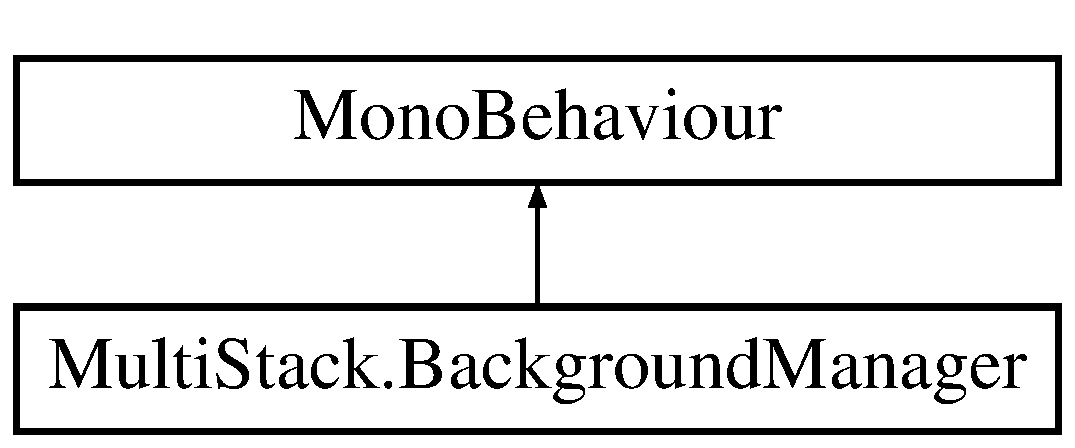
\includegraphics[height=2.000000cm]{class_multi_stack_1_1_background_manager}
\end{center}
\end{figure}
\subsection*{Public Attributes}
\begin{DoxyCompactItemize}
\item 
\hyperlink{struct_multi_stack_1_1_background}{Background}\mbox{[}$\,$\mbox{]} \hyperlink{class_multi_stack_1_1_background_manager_a44be514f6a5699866194bd0d28c6deaf}{backgrounds}
\begin{DoxyCompactList}\small\item\em The possible background objects. \end{DoxyCompactList}\end{DoxyCompactItemize}


\subsection{Detailed Description}
Creates the background object at runtime. Selects background from a pool of possible backgrounds. 



\subsection{Member Data Documentation}
\hypertarget{class_multi_stack_1_1_background_manager_a44be514f6a5699866194bd0d28c6deaf}{}\index{Multi\+Stack\+::\+Background\+Manager@{Multi\+Stack\+::\+Background\+Manager}!backgrounds@{backgrounds}}
\index{backgrounds@{backgrounds}!Multi\+Stack\+::\+Background\+Manager@{Multi\+Stack\+::\+Background\+Manager}}
\subsubsection[{backgrounds}]{\setlength{\rightskip}{0pt plus 5cm}{\bf Background} \mbox{[}$\,$\mbox{]} Multi\+Stack.\+Background\+Manager.\+backgrounds}\label{class_multi_stack_1_1_background_manager_a44be514f6a5699866194bd0d28c6deaf}


The possible background objects. 



The documentation for this class was generated from the following file\+:\begin{DoxyCompactItemize}
\item 
Multiplayer\+Stacker/\+Scripts/\+Environment/\+Background/Background\+Manager.\+cs\end{DoxyCompactItemize}

\hypertarget{class_multi_stack_1_1_camera_manager}{}\section{Multi\+Stack.\+Camera\+Manager Class Reference}
\label{class_multi_stack_1_1_camera_manager}\index{Multi\+Stack.\+Camera\+Manager@{Multi\+Stack.\+Camera\+Manager}}


Attached to the main camera in the Game Scene. Handles camera movement on the y axis.  


Inheritance diagram for Multi\+Stack.\+Camera\+Manager\+:\begin{figure}[H]
\begin{center}
\leavevmode
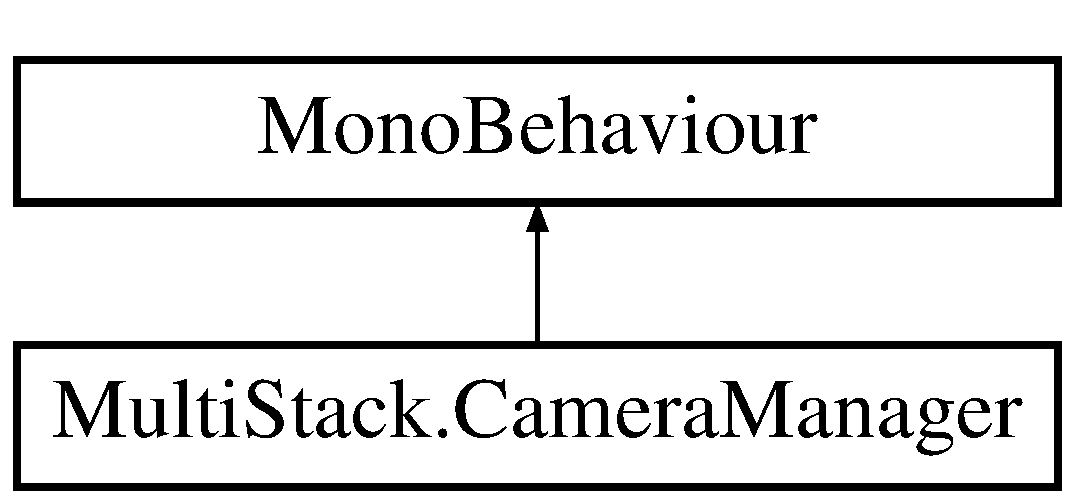
\includegraphics[height=2.000000cm]{class_multi_stack_1_1_camera_manager}
\end{center}
\end{figure}
\subsection*{Public Member Functions}
\begin{DoxyCompactItemize}
\item 
void \hyperlink{class_multi_stack_1_1_camera_manager_abe622bf707f58b977ae6535b848dc184}{Request\+New\+Target} (float target)
\begin{DoxyCompactList}\small\item\em Requests a new target y position. Confines camera movement to specific areas dependent on current stack height. Limits target position to within +/-\/ 1.\+5f of current target, not higher than the stacked shapes + 3f, and greater than 0. \end{DoxyCompactList}\item 
void \hyperlink{class_multi_stack_1_1_camera_manager_a081a72450ee5183b5945c49b5757e6db}{Set\+Target} (float target, float panspeed=1f)
\begin{DoxyCompactList}\small\item\em Sets the a new target y position. No constraints are placed on target. \end{DoxyCompactList}\item 
void \hyperlink{class_multi_stack_1_1_camera_manager_a591dc3386c3ba31118b694ded94c3e6f}{Reset\+Target} (float pan\+Speed\+To\+Target=1f)
\begin{DoxyCompactList}\small\item\em Resets the target y position to 0. \end{DoxyCompactList}\item 
void \hyperlink{class_multi_stack_1_1_camera_manager_aa13e9d644f4c815804224367467021c1}{Start\+Panning} (float pan\+Speed=1f)
\begin{DoxyCompactList}\small\item\em Begins camera movement. \end{DoxyCompactList}\item 
void \hyperlink{class_multi_stack_1_1_camera_manager_a3085f8ea5bbe1beb88a3219eba1e51bf}{Call\+Back\+On\+Target\+Reached} (\hyperlink{namespace_multi_stack_a4bd4097b52deebcafccf5815a8495960}{Call\+Back} call\+Back)
\begin{DoxyCompactList}\small\item\em Injects a method to be called when target is reached. Method is invoked once when target reached and then set to null. Call this method before setting a new target. \end{DoxyCompactList}\item 
void \hyperlink{class_multi_stack_1_1_camera_manager_a3625d7638336b34316ffc10bfa84eddd}{Reset\+Pan\+Speed\+On\+Target\+Reached} ()
\begin{DoxyCompactList}\small\item\em Camera movement speed is reset when target has been reached. Call this before setting a new target if you want the camera movement speed to return to its previous value. \end{DoxyCompactList}\end{DoxyCompactItemize}
\subsection*{Public Attributes}
\begin{DoxyCompactItemize}
\item 
float \hyperlink{class_multi_stack_1_1_camera_manager_a8dc8d08acda20d2098ca43430582199b}{target\+Y} = 0
\begin{DoxyCompactList}\small\item\em The target y position. \end{DoxyCompactList}\end{DoxyCompactItemize}
\subsection*{Properties}
\begin{DoxyCompactItemize}
\item 
bool \hyperlink{class_multi_stack_1_1_camera_manager_a47e71a3bf314c2f2dba156fc47e26127}{has\+Reached\+Target}\hspace{0.3cm}{\ttfamily  \mbox{[}get\mbox{]}}
\begin{DoxyCompactList}\small\item\em Gets a value indicating whether this \hyperlink{class_multi_stack_1_1_camera_manager}{Multi\+Stack.\+Camera\+Manager} has come within 0.\+2f of target y position. \end{DoxyCompactList}\item 
bool \hyperlink{class_multi_stack_1_1_camera_manager_aa36c3004b512594116595bc980734321}{should\+Pan}\hspace{0.3cm}{\ttfamily  \mbox{[}set\mbox{]}}
\begin{DoxyCompactList}\small\item\em Sets a value indicating whether this \hyperlink{class_multi_stack_1_1_camera_manager}{Multi\+Stack.\+Camera\+Manager} should pan to target y position. \end{DoxyCompactList}\end{DoxyCompactItemize}


\subsection{Detailed Description}
Attached to the main camera in the Game Scene. Handles camera movement on the y axis. 



\subsection{Member Function Documentation}
\hypertarget{class_multi_stack_1_1_camera_manager_a3085f8ea5bbe1beb88a3219eba1e51bf}{}\index{Multi\+Stack\+::\+Camera\+Manager@{Multi\+Stack\+::\+Camera\+Manager}!Call\+Back\+On\+Target\+Reached@{Call\+Back\+On\+Target\+Reached}}
\index{Call\+Back\+On\+Target\+Reached@{Call\+Back\+On\+Target\+Reached}!Multi\+Stack\+::\+Camera\+Manager@{Multi\+Stack\+::\+Camera\+Manager}}
\subsubsection[{Call\+Back\+On\+Target\+Reached(\+Call\+Back call\+Back)}]{\setlength{\rightskip}{0pt plus 5cm}void Multi\+Stack.\+Camera\+Manager.\+Call\+Back\+On\+Target\+Reached (
\begin{DoxyParamCaption}
\item[{{\bf Call\+Back}}]{call\+Back}
\end{DoxyParamCaption}
)}\label{class_multi_stack_1_1_camera_manager_a3085f8ea5bbe1beb88a3219eba1e51bf}


Injects a method to be called when target is reached. Method is invoked once when target reached and then set to null. Call this method before setting a new target. 


\begin{DoxyParams}{Parameters}
{\em call\+Back} & Call back.\\
\hline
\end{DoxyParams}
\hypertarget{class_multi_stack_1_1_camera_manager_abe622bf707f58b977ae6535b848dc184}{}\index{Multi\+Stack\+::\+Camera\+Manager@{Multi\+Stack\+::\+Camera\+Manager}!Request\+New\+Target@{Request\+New\+Target}}
\index{Request\+New\+Target@{Request\+New\+Target}!Multi\+Stack\+::\+Camera\+Manager@{Multi\+Stack\+::\+Camera\+Manager}}
\subsubsection[{Request\+New\+Target(float target)}]{\setlength{\rightskip}{0pt plus 5cm}void Multi\+Stack.\+Camera\+Manager.\+Request\+New\+Target (
\begin{DoxyParamCaption}
\item[{float}]{target}
\end{DoxyParamCaption}
)}\label{class_multi_stack_1_1_camera_manager_abe622bf707f58b977ae6535b848dc184}


Requests a new target y position. Confines camera movement to specific areas dependent on current stack height. Limits target position to within +/-\/ 1.\+5f of current target, not higher than the stacked shapes + 3f, and greater than 0. 


\begin{DoxyParams}{Parameters}
{\em target} & Target y position.\\
\hline
\end{DoxyParams}
\hypertarget{class_multi_stack_1_1_camera_manager_a3625d7638336b34316ffc10bfa84eddd}{}\index{Multi\+Stack\+::\+Camera\+Manager@{Multi\+Stack\+::\+Camera\+Manager}!Reset\+Pan\+Speed\+On\+Target\+Reached@{Reset\+Pan\+Speed\+On\+Target\+Reached}}
\index{Reset\+Pan\+Speed\+On\+Target\+Reached@{Reset\+Pan\+Speed\+On\+Target\+Reached}!Multi\+Stack\+::\+Camera\+Manager@{Multi\+Stack\+::\+Camera\+Manager}}
\subsubsection[{Reset\+Pan\+Speed\+On\+Target\+Reached()}]{\setlength{\rightskip}{0pt plus 5cm}void Multi\+Stack.\+Camera\+Manager.\+Reset\+Pan\+Speed\+On\+Target\+Reached (
\begin{DoxyParamCaption}
{}
\end{DoxyParamCaption}
)}\label{class_multi_stack_1_1_camera_manager_a3625d7638336b34316ffc10bfa84eddd}


Camera movement speed is reset when target has been reached. Call this before setting a new target if you want the camera movement speed to return to its previous value. 

\hypertarget{class_multi_stack_1_1_camera_manager_a591dc3386c3ba31118b694ded94c3e6f}{}\index{Multi\+Stack\+::\+Camera\+Manager@{Multi\+Stack\+::\+Camera\+Manager}!Reset\+Target@{Reset\+Target}}
\index{Reset\+Target@{Reset\+Target}!Multi\+Stack\+::\+Camera\+Manager@{Multi\+Stack\+::\+Camera\+Manager}}
\subsubsection[{Reset\+Target(float pan\+Speed\+To\+Target=1f)}]{\setlength{\rightskip}{0pt plus 5cm}void Multi\+Stack.\+Camera\+Manager.\+Reset\+Target (
\begin{DoxyParamCaption}
\item[{float}]{pan\+Speed\+To\+Target = {\ttfamily 1f}}
\end{DoxyParamCaption}
)}\label{class_multi_stack_1_1_camera_manager_a591dc3386c3ba31118b694ded94c3e6f}


Resets the target y position to 0. 


\begin{DoxyParams}{Parameters}
{\em pan\+Speed\+To\+Target} & Pan speed to target.\\
\hline
\end{DoxyParams}
\hypertarget{class_multi_stack_1_1_camera_manager_a081a72450ee5183b5945c49b5757e6db}{}\index{Multi\+Stack\+::\+Camera\+Manager@{Multi\+Stack\+::\+Camera\+Manager}!Set\+Target@{Set\+Target}}
\index{Set\+Target@{Set\+Target}!Multi\+Stack\+::\+Camera\+Manager@{Multi\+Stack\+::\+Camera\+Manager}}
\subsubsection[{Set\+Target(float target, float panspeed=1f)}]{\setlength{\rightskip}{0pt plus 5cm}void Multi\+Stack.\+Camera\+Manager.\+Set\+Target (
\begin{DoxyParamCaption}
\item[{float}]{target, }
\item[{float}]{panspeed = {\ttfamily 1f}}
\end{DoxyParamCaption}
)}\label{class_multi_stack_1_1_camera_manager_a081a72450ee5183b5945c49b5757e6db}


Sets the a new target y position. No constraints are placed on target. 


\begin{DoxyParams}{Parameters}
{\em target} & Target.\\
\hline
{\em panspeed} & The speed to move to new target.\\
\hline
\end{DoxyParams}
\hypertarget{class_multi_stack_1_1_camera_manager_aa13e9d644f4c815804224367467021c1}{}\index{Multi\+Stack\+::\+Camera\+Manager@{Multi\+Stack\+::\+Camera\+Manager}!Start\+Panning@{Start\+Panning}}
\index{Start\+Panning@{Start\+Panning}!Multi\+Stack\+::\+Camera\+Manager@{Multi\+Stack\+::\+Camera\+Manager}}
\subsubsection[{Start\+Panning(float pan\+Speed=1f)}]{\setlength{\rightskip}{0pt plus 5cm}void Multi\+Stack.\+Camera\+Manager.\+Start\+Panning (
\begin{DoxyParamCaption}
\item[{float}]{pan\+Speed = {\ttfamily 1f}}
\end{DoxyParamCaption}
)}\label{class_multi_stack_1_1_camera_manager_aa13e9d644f4c815804224367467021c1}


Begins camera movement. 


\begin{DoxyParams}{Parameters}
{\em pan\+Speed} & Pan speed to target.\\
\hline
\end{DoxyParams}


\subsection{Member Data Documentation}
\hypertarget{class_multi_stack_1_1_camera_manager_a8dc8d08acda20d2098ca43430582199b}{}\index{Multi\+Stack\+::\+Camera\+Manager@{Multi\+Stack\+::\+Camera\+Manager}!target\+Y@{target\+Y}}
\index{target\+Y@{target\+Y}!Multi\+Stack\+::\+Camera\+Manager@{Multi\+Stack\+::\+Camera\+Manager}}
\subsubsection[{target\+Y}]{\setlength{\rightskip}{0pt plus 5cm}float Multi\+Stack.\+Camera\+Manager.\+target\+Y = 0}\label{class_multi_stack_1_1_camera_manager_a8dc8d08acda20d2098ca43430582199b}


The target y position. 



\subsection{Property Documentation}
\hypertarget{class_multi_stack_1_1_camera_manager_a47e71a3bf314c2f2dba156fc47e26127}{}\index{Multi\+Stack\+::\+Camera\+Manager@{Multi\+Stack\+::\+Camera\+Manager}!has\+Reached\+Target@{has\+Reached\+Target}}
\index{has\+Reached\+Target@{has\+Reached\+Target}!Multi\+Stack\+::\+Camera\+Manager@{Multi\+Stack\+::\+Camera\+Manager}}
\subsubsection[{has\+Reached\+Target}]{\setlength{\rightskip}{0pt plus 5cm}bool Multi\+Stack.\+Camera\+Manager.\+has\+Reached\+Target\hspace{0.3cm}{\ttfamily [get]}}\label{class_multi_stack_1_1_camera_manager_a47e71a3bf314c2f2dba156fc47e26127}


Gets a value indicating whether this \hyperlink{class_multi_stack_1_1_camera_manager}{Multi\+Stack.\+Camera\+Manager} has come within 0.\+2f of target y position. 

{\ttfamily true} if has reached target; otherwise, {\ttfamily false}.\hypertarget{class_multi_stack_1_1_camera_manager_aa36c3004b512594116595bc980734321}{}\index{Multi\+Stack\+::\+Camera\+Manager@{Multi\+Stack\+::\+Camera\+Manager}!should\+Pan@{should\+Pan}}
\index{should\+Pan@{should\+Pan}!Multi\+Stack\+::\+Camera\+Manager@{Multi\+Stack\+::\+Camera\+Manager}}
\subsubsection[{should\+Pan}]{\setlength{\rightskip}{0pt plus 5cm}bool Multi\+Stack.\+Camera\+Manager.\+should\+Pan\hspace{0.3cm}{\ttfamily [set]}}\label{class_multi_stack_1_1_camera_manager_aa36c3004b512594116595bc980734321}


Sets a value indicating whether this \hyperlink{class_multi_stack_1_1_camera_manager}{Multi\+Stack.\+Camera\+Manager} should pan to target y position. 

{\ttfamily true} if should pan; otherwise, {\ttfamily false}.

The documentation for this class was generated from the following file\+:\begin{DoxyCompactItemize}
\item 
Multiplayer\+Stacker/\+Scripts/\+Camera/Camera\+Manager.\+cs\end{DoxyCompactItemize}

\hypertarget{class_multi_stack_1_1_camera_shake}{}\section{Multi\+Stack.\+Camera\+Shake Class Reference}
\label{class_multi_stack_1_1_camera_shake}\index{Multi\+Stack.\+Camera\+Shake@{Multi\+Stack.\+Camera\+Shake}}


Handles camera shake on explosion.  


Inheritance diagram for Multi\+Stack.\+Camera\+Shake\+:\begin{figure}[H]
\begin{center}
\leavevmode
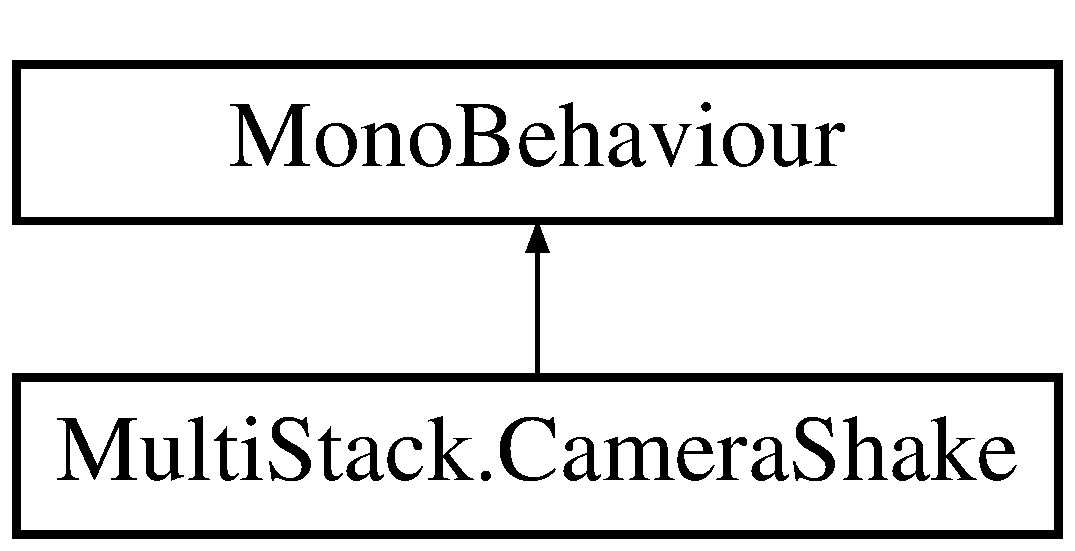
\includegraphics[height=2.000000cm]{class_multi_stack_1_1_camera_shake}
\end{center}
\end{figure}
\subsection*{Public Member Functions}
\begin{DoxyCompactItemize}
\item 
void \hyperlink{class_multi_stack_1_1_camera_shake_a6571236e5ca1ba88f0a3114f9357e8f4}{Shake} (float shake\+Intensity=0.\+05f, float shake\+Decay=0.\+004f)
\begin{DoxyCompactList}\small\item\em Begins the shake effect with the desired intensity and decay. \end{DoxyCompactList}\end{DoxyCompactItemize}


\subsection{Detailed Description}
Handles camera shake on explosion. 



\subsection{Member Function Documentation}
\hypertarget{class_multi_stack_1_1_camera_shake_a6571236e5ca1ba88f0a3114f9357e8f4}{}\index{Multi\+Stack\+::\+Camera\+Shake@{Multi\+Stack\+::\+Camera\+Shake}!Shake@{Shake}}
\index{Shake@{Shake}!Multi\+Stack\+::\+Camera\+Shake@{Multi\+Stack\+::\+Camera\+Shake}}
\subsubsection[{Shake(float shake\+Intensity=0.\+05f, float shake\+Decay=0.\+004f)}]{\setlength{\rightskip}{0pt plus 5cm}void Multi\+Stack.\+Camera\+Shake.\+Shake (
\begin{DoxyParamCaption}
\item[{float}]{shake\+Intensity = {\ttfamily 0.05f}, }
\item[{float}]{shake\+Decay = {\ttfamily 0.004f}}
\end{DoxyParamCaption}
)}\label{class_multi_stack_1_1_camera_shake_a6571236e5ca1ba88f0a3114f9357e8f4}


Begins the shake effect with the desired intensity and decay. 


\begin{DoxyParams}{Parameters}
{\em shake\+Intensity} & Shake intensity.\\
\hline
{\em shake\+Decay} & Shake decay.\\
\hline
\end{DoxyParams}


The documentation for this class was generated from the following file\+:\begin{DoxyCompactItemize}
\item 
Multiplayer\+Stacker/\+Scripts/\+U\+I/Camera\+Shake.\+cs\end{DoxyCompactItemize}

\hypertarget{class_multi_stack_1_1_can_only_pickup_once_modifier}{}\section{Multi\+Stack.\+Can\+Only\+Pickup\+Once\+Modifier Class Reference}
\label{class_multi_stack_1_1_can_only_pickup_once_modifier}\index{Multi\+Stack.\+Can\+Only\+Pickup\+Once\+Modifier@{Multi\+Stack.\+Can\+Only\+Pickup\+Once\+Modifier}}


When enabled the player can only pickup a shape once. Once a shape is dropped it is no longer draggable. Invokes \hyperlink{class_multi_stack_1_1_click_handler_ab7cdf9c5b65265b0f17437ee6313fbeb}{Multi\+Stack.\+Click\+Handler.\+can\+Only\+Click\+Once}  


Inheritance diagram for Multi\+Stack.\+Can\+Only\+Pickup\+Once\+Modifier\+:\begin{figure}[H]
\begin{center}
\leavevmode
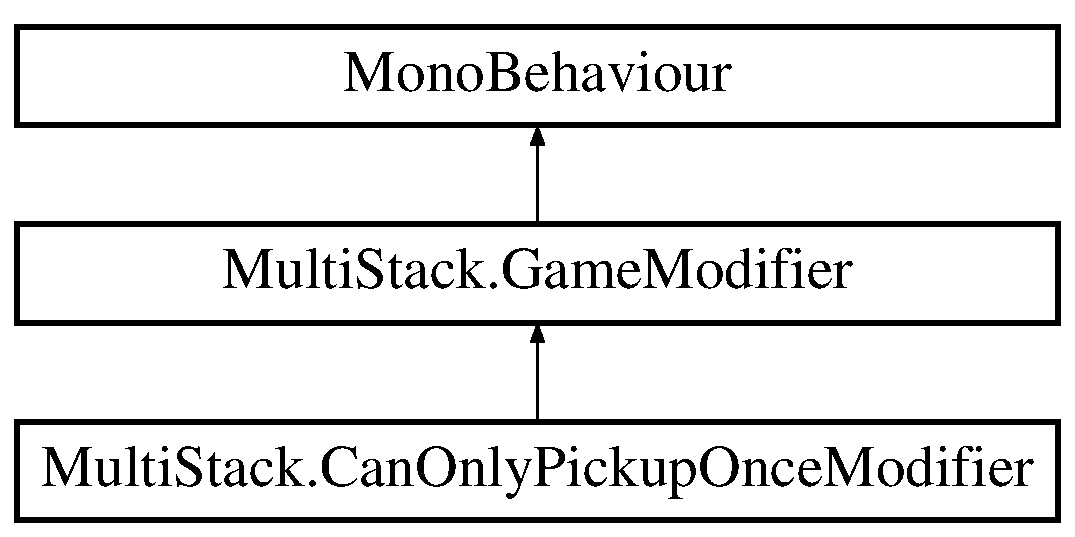
\includegraphics[height=3.000000cm]{class_multi_stack_1_1_can_only_pickup_once_modifier}
\end{center}
\end{figure}
\subsection*{Public Member Functions}
\begin{DoxyCompactItemize}
\item 
override void \hyperlink{class_multi_stack_1_1_can_only_pickup_once_modifier_a92da95d7bb53c6c81c60a0a0d28b5c1b}{Activate} ()
\begin{DoxyCompactList}\small\item\em Activate this modifier. Called at the beginning of the round. \end{DoxyCompactList}\item 
override void \hyperlink{class_multi_stack_1_1_can_only_pickup_once_modifier_a5375d39256e231f65b9dddc86581b185}{Deactivate} ()
\begin{DoxyCompactList}\small\item\em Deactivate this modifier. Called before a new modifier is enabled. \end{DoxyCompactList}\end{DoxyCompactItemize}
\subsection*{Public Attributes}
\begin{DoxyCompactItemize}
\item 
\hypertarget{class_multi_stack_1_1_can_only_pickup_once_modifier_ad5273072c26e70616347a79d7701292d}{}\hyperlink{class_multi_stack_1_1_click_handler}{Click\+Handler} {\bfseries click\+Handler}\label{class_multi_stack_1_1_can_only_pickup_once_modifier_ad5273072c26e70616347a79d7701292d}

\end{DoxyCompactItemize}


\subsection{Detailed Description}
When enabled the player can only pickup a shape once. Once a shape is dropped it is no longer draggable. Invokes \hyperlink{class_multi_stack_1_1_click_handler_ab7cdf9c5b65265b0f17437ee6313fbeb}{Multi\+Stack.\+Click\+Handler.\+can\+Only\+Click\+Once} 



\subsection{Member Function Documentation}
\hypertarget{class_multi_stack_1_1_can_only_pickup_once_modifier_a92da95d7bb53c6c81c60a0a0d28b5c1b}{}\index{Multi\+Stack\+::\+Can\+Only\+Pickup\+Once\+Modifier@{Multi\+Stack\+::\+Can\+Only\+Pickup\+Once\+Modifier}!Activate@{Activate}}
\index{Activate@{Activate}!Multi\+Stack\+::\+Can\+Only\+Pickup\+Once\+Modifier@{Multi\+Stack\+::\+Can\+Only\+Pickup\+Once\+Modifier}}
\subsubsection[{Activate()}]{\setlength{\rightskip}{0pt plus 5cm}override void Multi\+Stack.\+Can\+Only\+Pickup\+Once\+Modifier.\+Activate (
\begin{DoxyParamCaption}
{}
\end{DoxyParamCaption}
)\hspace{0.3cm}{\ttfamily [virtual]}}\label{class_multi_stack_1_1_can_only_pickup_once_modifier_a92da95d7bb53c6c81c60a0a0d28b5c1b}


Activate this modifier. Called at the beginning of the round. 



Implements \hyperlink{class_multi_stack_1_1_game_modifier_a3fb880f9728f8680bf473ac5c7f6832e}{Multi\+Stack.\+Game\+Modifier}.

\hypertarget{class_multi_stack_1_1_can_only_pickup_once_modifier_a5375d39256e231f65b9dddc86581b185}{}\index{Multi\+Stack\+::\+Can\+Only\+Pickup\+Once\+Modifier@{Multi\+Stack\+::\+Can\+Only\+Pickup\+Once\+Modifier}!Deactivate@{Deactivate}}
\index{Deactivate@{Deactivate}!Multi\+Stack\+::\+Can\+Only\+Pickup\+Once\+Modifier@{Multi\+Stack\+::\+Can\+Only\+Pickup\+Once\+Modifier}}
\subsubsection[{Deactivate()}]{\setlength{\rightskip}{0pt plus 5cm}override void Multi\+Stack.\+Can\+Only\+Pickup\+Once\+Modifier.\+Deactivate (
\begin{DoxyParamCaption}
{}
\end{DoxyParamCaption}
)\hspace{0.3cm}{\ttfamily [virtual]}}\label{class_multi_stack_1_1_can_only_pickup_once_modifier_a5375d39256e231f65b9dddc86581b185}


Deactivate this modifier. Called before a new modifier is enabled. 



Implements \hyperlink{class_multi_stack_1_1_game_modifier_abe04db6ab31f5e5063739d8e5a3f7ad1}{Multi\+Stack.\+Game\+Modifier}.



The documentation for this class was generated from the following file\+:\begin{DoxyCompactItemize}
\item 
Multiplayer\+Stacker/\+Scripts/\+Modifiers/Can\+Only\+Pickup\+Once\+Modifier.\+cs\end{DoxyCompactItemize}

\hypertarget{class_multi_stack_1_1_catch_the_shape_modifier}{}\section{Multi\+Stack.\+Catch\+The\+Shape\+Modifier Class Reference}
\label{class_multi_stack_1_1_catch_the_shape_modifier}\index{Multi\+Stack.\+Catch\+The\+Shape\+Modifier@{Multi\+Stack.\+Catch\+The\+Shape\+Modifier}}


When enabled any newly spawned physics objects are dropped straight away rather than waiting for the player to click on/touch them.  


Inheritance diagram for Multi\+Stack.\+Catch\+The\+Shape\+Modifier\+:\begin{figure}[H]
\begin{center}
\leavevmode
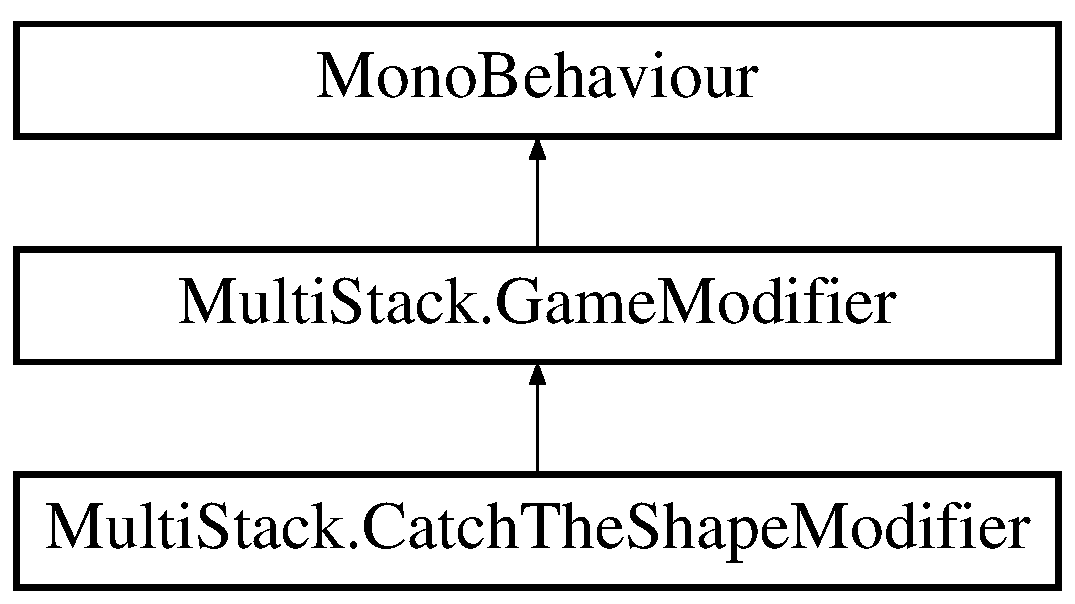
\includegraphics[height=3.000000cm]{class_multi_stack_1_1_catch_the_shape_modifier}
\end{center}
\end{figure}
\subsection*{Public Member Functions}
\begin{DoxyCompactItemize}
\item 
override void \hyperlink{class_multi_stack_1_1_catch_the_shape_modifier_a5617ebd934298acc024336daa5c633fb}{Activate} ()
\begin{DoxyCompactList}\small\item\em Activate this modifier. Called at the beginning of the round. \end{DoxyCompactList}\item 
override void \hyperlink{class_multi_stack_1_1_catch_the_shape_modifier_ad6ad792bcc0ae5fdd4890af7ec5fe7b1}{Deactivate} ()
\begin{DoxyCompactList}\small\item\em Deactivate this modifier. Called before a new modifier is enabled. \end{DoxyCompactList}\end{DoxyCompactItemize}
\subsection*{Additional Inherited Members}


\subsection{Detailed Description}
When enabled any newly spawned physics objects are dropped straight away rather than waiting for the player to click on/touch them. 



\subsection{Member Function Documentation}
\hypertarget{class_multi_stack_1_1_catch_the_shape_modifier_a5617ebd934298acc024336daa5c633fb}{}\index{Multi\+Stack\+::\+Catch\+The\+Shape\+Modifier@{Multi\+Stack\+::\+Catch\+The\+Shape\+Modifier}!Activate@{Activate}}
\index{Activate@{Activate}!Multi\+Stack\+::\+Catch\+The\+Shape\+Modifier@{Multi\+Stack\+::\+Catch\+The\+Shape\+Modifier}}
\subsubsection[{Activate()}]{\setlength{\rightskip}{0pt plus 5cm}override void Multi\+Stack.\+Catch\+The\+Shape\+Modifier.\+Activate (
\begin{DoxyParamCaption}
{}
\end{DoxyParamCaption}
)\hspace{0.3cm}{\ttfamily [virtual]}}\label{class_multi_stack_1_1_catch_the_shape_modifier_a5617ebd934298acc024336daa5c633fb}


Activate this modifier. Called at the beginning of the round. 



Implements \hyperlink{class_multi_stack_1_1_game_modifier_a3fb880f9728f8680bf473ac5c7f6832e}{Multi\+Stack.\+Game\+Modifier}.

\hypertarget{class_multi_stack_1_1_catch_the_shape_modifier_ad6ad792bcc0ae5fdd4890af7ec5fe7b1}{}\index{Multi\+Stack\+::\+Catch\+The\+Shape\+Modifier@{Multi\+Stack\+::\+Catch\+The\+Shape\+Modifier}!Deactivate@{Deactivate}}
\index{Deactivate@{Deactivate}!Multi\+Stack\+::\+Catch\+The\+Shape\+Modifier@{Multi\+Stack\+::\+Catch\+The\+Shape\+Modifier}}
\subsubsection[{Deactivate()}]{\setlength{\rightskip}{0pt plus 5cm}override void Multi\+Stack.\+Catch\+The\+Shape\+Modifier.\+Deactivate (
\begin{DoxyParamCaption}
{}
\end{DoxyParamCaption}
)\hspace{0.3cm}{\ttfamily [virtual]}}\label{class_multi_stack_1_1_catch_the_shape_modifier_ad6ad792bcc0ae5fdd4890af7ec5fe7b1}


Deactivate this modifier. Called before a new modifier is enabled. 



Implements \hyperlink{class_multi_stack_1_1_game_modifier_abe04db6ab31f5e5063739d8e5a3f7ad1}{Multi\+Stack.\+Game\+Modifier}.



The documentation for this class was generated from the following file\+:\begin{DoxyCompactItemize}
\item 
Multiplayer\+Stacker/\+Scripts/\+Modifiers/Catch\+The\+Shape\+Modifier.\+cs\end{DoxyCompactItemize}

\hypertarget{class_multi_stack_1_1_clickable_object}{}\section{Multi\+Stack.\+Clickable\+Object Class Reference}
\label{class_multi_stack_1_1_clickable_object}\index{Multi\+Stack.\+Clickable\+Object@{Multi\+Stack.\+Clickable\+Object}}


Attached to all physics objects. Defines if a object is currently being held. Used by \hyperlink{class_multi_stack_1_1_turn_manager}{Multi\+Stack.\+Turn\+Manager} to help decide if a players turn is over. Also used to turn off interaction with object by setting \hyperlink{class_multi_stack_1_1_clickable_object_a9fbbe82e73f95769344946b8b39e2520}{Multi\+Stack.\+Clickable\+Object.\+clickable}  


Inheritance diagram for Multi\+Stack.\+Clickable\+Object\+:\begin{figure}[H]
\begin{center}
\leavevmode
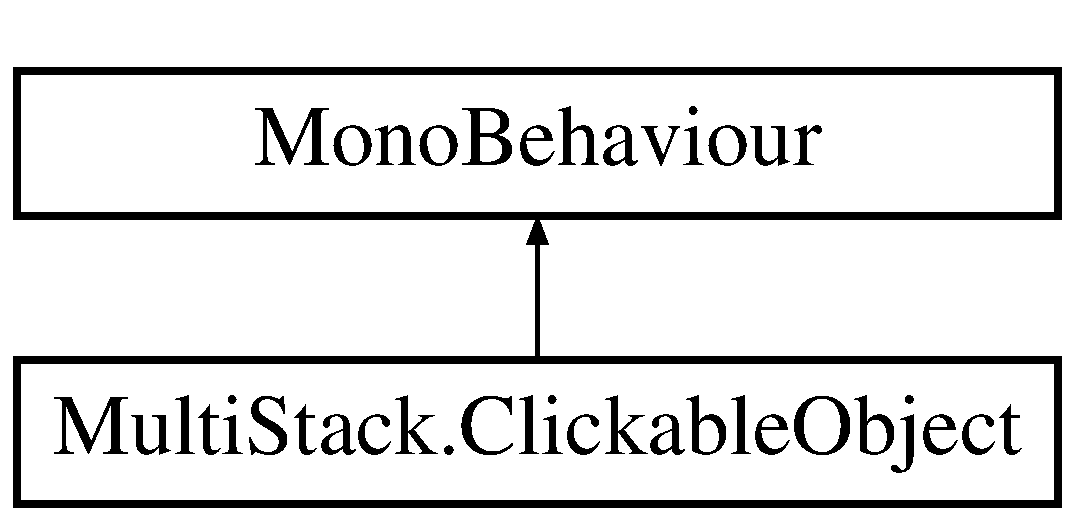
\includegraphics[height=2.000000cm]{class_multi_stack_1_1_clickable_object}
\end{center}
\end{figure}
\subsection*{Public Member Functions}
\begin{DoxyCompactItemize}
\item 
void \hyperlink{class_multi_stack_1_1_clickable_object_ae6b5da3e366e61daac3031b9643a780e}{Clicked} ()
\begin{DoxyCompactList}\small\item\em Physics obkect has been \textquotesingle{}clicked\textquotesingle{} on. \end{DoxyCompactList}\end{DoxyCompactItemize}
\subsection*{Properties}
\begin{DoxyCompactItemize}
\item 
bool \hyperlink{class_multi_stack_1_1_clickable_object_a9fbbe82e73f95769344946b8b39e2520}{clickable}\hspace{0.3cm}{\ttfamily  \mbox{[}get\mbox{]}}
\begin{DoxyCompactList}\small\item\em Gets a value indicating whether this \hyperlink{class_multi_stack_1_1_clickable_object}{Multi\+Stack.\+Clickable\+Object} is selectable. \end{DoxyCompactList}\end{DoxyCompactItemize}


\subsection{Detailed Description}
Attached to all physics objects. Defines if a object is currently being held. Used by \hyperlink{class_multi_stack_1_1_turn_manager}{Multi\+Stack.\+Turn\+Manager} to help decide if a players turn is over. Also used to turn off interaction with object by setting \hyperlink{class_multi_stack_1_1_clickable_object_a9fbbe82e73f95769344946b8b39e2520}{Multi\+Stack.\+Clickable\+Object.\+clickable} 



\subsection{Member Function Documentation}
\hypertarget{class_multi_stack_1_1_clickable_object_ae6b5da3e366e61daac3031b9643a780e}{}\index{Multi\+Stack\+::\+Clickable\+Object@{Multi\+Stack\+::\+Clickable\+Object}!Clicked@{Clicked}}
\index{Clicked@{Clicked}!Multi\+Stack\+::\+Clickable\+Object@{Multi\+Stack\+::\+Clickable\+Object}}
\subsubsection[{Clicked()}]{\setlength{\rightskip}{0pt plus 5cm}void Multi\+Stack.\+Clickable\+Object.\+Clicked (
\begin{DoxyParamCaption}
{}
\end{DoxyParamCaption}
)}\label{class_multi_stack_1_1_clickable_object_ae6b5da3e366e61daac3031b9643a780e}


Physics obkect has been \textquotesingle{}clicked\textquotesingle{} on. 



\subsection{Property Documentation}
\hypertarget{class_multi_stack_1_1_clickable_object_a9fbbe82e73f95769344946b8b39e2520}{}\index{Multi\+Stack\+::\+Clickable\+Object@{Multi\+Stack\+::\+Clickable\+Object}!clickable@{clickable}}
\index{clickable@{clickable}!Multi\+Stack\+::\+Clickable\+Object@{Multi\+Stack\+::\+Clickable\+Object}}
\subsubsection[{clickable}]{\setlength{\rightskip}{0pt plus 5cm}bool Multi\+Stack.\+Clickable\+Object.\+clickable\hspace{0.3cm}{\ttfamily [get]}}\label{class_multi_stack_1_1_clickable_object_a9fbbe82e73f95769344946b8b39e2520}


Gets a value indicating whether this \hyperlink{class_multi_stack_1_1_clickable_object}{Multi\+Stack.\+Clickable\+Object} is selectable. 

{\ttfamily true} if clickable; otherwise, {\ttfamily false}.

The documentation for this class was generated from the following file\+:\begin{DoxyCompactItemize}
\item 
Multiplayer\+Stacker/\+Scripts/Clickable\+Object.\+cs\end{DoxyCompactItemize}

\hypertarget{class_multi_stack_1_1_click_handler}{}\section{Multi\+Stack.\+Click\+Handler Class Reference}
\label{class_multi_stack_1_1_click_handler}\index{Multi\+Stack.\+Click\+Handler@{Multi\+Stack.\+Click\+Handler}}


The main click/drag manager. Handles picking up, dragging, and dropping of physics objects via mouse or touch screen controls.  


Inheritance diagram for Multi\+Stack.\+Click\+Handler\+:\begin{figure}[H]
\begin{center}
\leavevmode
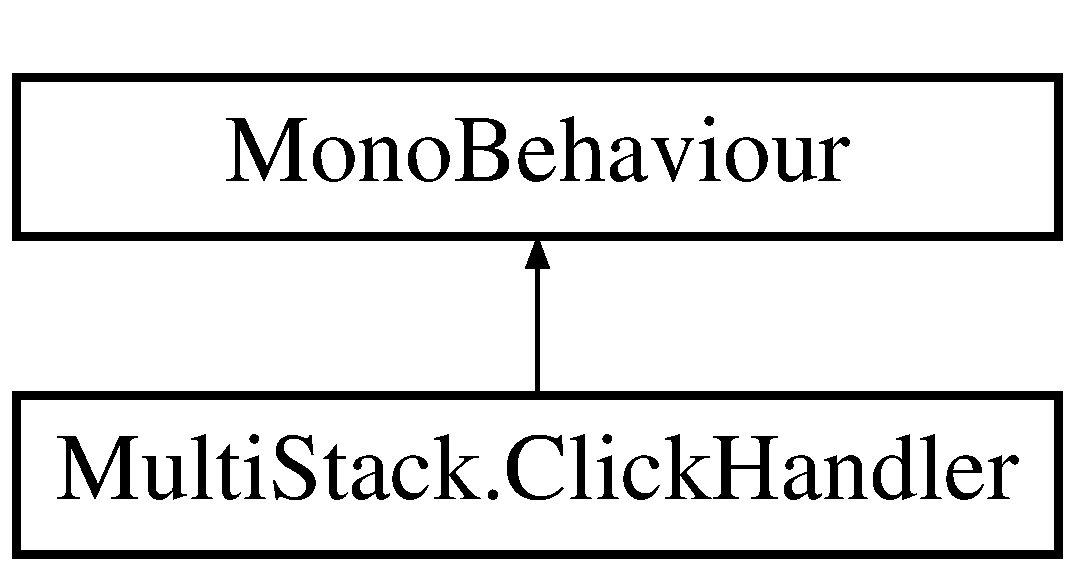
\includegraphics[height=2.000000cm]{class_multi_stack_1_1_click_handler}
\end{center}
\end{figure}
\subsection*{Public Attributes}
\begin{DoxyCompactItemize}
\item 
bool \hyperlink{class_multi_stack_1_1_click_handler_a2e0855046aafb6f87b298c83de1c82f5}{is\+Main\+Menu\+Scene} = false
\begin{DoxyCompactList}\small\item\em Sets whether this is main menu scene. Camera does not follow picked up objects if it is the main menu scene. \end{DoxyCompactList}\item 
Layer\+Mask \hyperlink{class_multi_stack_1_1_click_handler_a89cab89c49c38f4b96855de249618405}{box\+Mask}
\begin{DoxyCompactList}\small\item\em The layermask of the physics objects. \end{DoxyCompactList}\item 
Line\+Renderer \hyperlink{class_multi_stack_1_1_click_handler_a7d28187d20185f4b352669cbd072b3b5}{drag\+Line}
\begin{DoxyCompactList}\small\item\em The line renderer for the line drawn between cursor/finger and grabbed object. \end{DoxyCompactList}\item 
\hyperlink{class_multi_stack_1_1_player_colours}{Player\+Colours} \hyperlink{class_multi_stack_1_1_click_handler_a02d956303c6e5a958379602f9103add7}{player\+Colours}
\begin{DoxyCompactList}\small\item\em Reference to player colours, used to change the colour of \hyperlink{class_multi_stack_1_1_click_handler_a7d28187d20185f4b352669cbd072b3b5}{Multi\+Stack.\+Click\+Handler.\+drag\+Line} based on current player. \end{DoxyCompactList}\end{DoxyCompactItemize}
\subsection*{Properties}
\begin{DoxyCompactItemize}
\item 
bool \hyperlink{class_multi_stack_1_1_click_handler_ae1edbbbc7bc6fb0d73aac34fd5a47b48}{use\+Spring}\hspace{0.3cm}{\ttfamily  \mbox{[}get, set\mbox{]}}
\begin{DoxyCompactList}\small\item\em Gets or sets a value indicating whether this \hyperlink{class_multi_stack_1_1_click_handler}{Multi\+Stack.\+Click\+Handler} should use a spring when dragging an object. \end{DoxyCompactList}\item 
float \hyperlink{class_multi_stack_1_1_click_handler_a190adce119045b21706fefa1e0ad2b7b}{velocity\+Ratio}\hspace{0.3cm}{\ttfamily  \mbox{[}get, set\mbox{]}}
\begin{DoxyCompactList}\small\item\em Gets or sets the velocity ratio used when dragging an object. \end{DoxyCompactList}\item 
bool \hyperlink{class_multi_stack_1_1_click_handler_a77a3775355cbfd06654ca0740d3200e3}{drag\+Reversed}\hspace{0.3cm}{\ttfamily  \mbox{[}set\mbox{]}}
\begin{DoxyCompactList}\small\item\em Sets a value indicating whether this \hyperlink{class_multi_stack_1_1_click_handler}{Multi\+Stack.\+Click\+Handler} has reversed drag i.\+e. when the player drags right, the shape moves left. \end{DoxyCompactList}\item 
bool \hyperlink{class_multi_stack_1_1_click_handler_a9088a8092cd9c9525c7024a3e7070c77}{shakey\+Shapes}\hspace{0.3cm}{\ttfamily  \mbox{[}get, set\mbox{]}}
\begin{DoxyCompactList}\small\item\em Gets or sets a value indicating whether this \hyperlink{class_multi_stack_1_1_click_handler}{Multi\+Stack.\+Click\+Handler} should use shakey shapes. When enabled a random offset is added to the shapes position each time step. \end{DoxyCompactList}\item 
bool \hyperlink{class_multi_stack_1_1_click_handler_a7097c4cddc7a31d0a9d303c5367d10be}{increase\+Shape\+Size}\hspace{0.3cm}{\ttfamily  \mbox{[}get, set\mbox{]}}
\begin{DoxyCompactList}\small\item\em Gets or sets a value indicating whether this \hyperlink{class_multi_stack_1_1_click_handler}{Multi\+Stack.\+Click\+Handler} should increase shape size when a shape is held. \end{DoxyCompactList}\item 
bool \hyperlink{class_multi_stack_1_1_click_handler_ab7cdf9c5b65265b0f17437ee6313fbeb}{can\+Only\+Click\+Once}\hspace{0.3cm}{\ttfamily  \mbox{[}get, set\mbox{]}}
\begin{DoxyCompactList}\small\item\em Gets or sets a value indicating whether this \hyperlink{class_multi_stack_1_1_click_handler}{Multi\+Stack.\+Click\+Handler} can only grab an object once. \end{DoxyCompactList}\end{DoxyCompactItemize}


\subsection{Detailed Description}
The main click/drag manager. Handles picking up, dragging, and dropping of physics objects via mouse or touch screen controls. 



\subsection{Member Data Documentation}
\hypertarget{class_multi_stack_1_1_click_handler_a89cab89c49c38f4b96855de249618405}{}\index{Multi\+Stack\+::\+Click\+Handler@{Multi\+Stack\+::\+Click\+Handler}!box\+Mask@{box\+Mask}}
\index{box\+Mask@{box\+Mask}!Multi\+Stack\+::\+Click\+Handler@{Multi\+Stack\+::\+Click\+Handler}}
\subsubsection[{box\+Mask}]{\setlength{\rightskip}{0pt plus 5cm}Layer\+Mask Multi\+Stack.\+Click\+Handler.\+box\+Mask}\label{class_multi_stack_1_1_click_handler_a89cab89c49c38f4b96855de249618405}


The layermask of the physics objects. 

\hypertarget{class_multi_stack_1_1_click_handler_a7d28187d20185f4b352669cbd072b3b5}{}\index{Multi\+Stack\+::\+Click\+Handler@{Multi\+Stack\+::\+Click\+Handler}!drag\+Line@{drag\+Line}}
\index{drag\+Line@{drag\+Line}!Multi\+Stack\+::\+Click\+Handler@{Multi\+Stack\+::\+Click\+Handler}}
\subsubsection[{drag\+Line}]{\setlength{\rightskip}{0pt plus 5cm}Line\+Renderer Multi\+Stack.\+Click\+Handler.\+drag\+Line}\label{class_multi_stack_1_1_click_handler_a7d28187d20185f4b352669cbd072b3b5}


The line renderer for the line drawn between cursor/finger and grabbed object. 

\hypertarget{class_multi_stack_1_1_click_handler_a2e0855046aafb6f87b298c83de1c82f5}{}\index{Multi\+Stack\+::\+Click\+Handler@{Multi\+Stack\+::\+Click\+Handler}!is\+Main\+Menu\+Scene@{is\+Main\+Menu\+Scene}}
\index{is\+Main\+Menu\+Scene@{is\+Main\+Menu\+Scene}!Multi\+Stack\+::\+Click\+Handler@{Multi\+Stack\+::\+Click\+Handler}}
\subsubsection[{is\+Main\+Menu\+Scene}]{\setlength{\rightskip}{0pt plus 5cm}bool Multi\+Stack.\+Click\+Handler.\+is\+Main\+Menu\+Scene = false}\label{class_multi_stack_1_1_click_handler_a2e0855046aafb6f87b298c83de1c82f5}


Sets whether this is main menu scene. Camera does not follow picked up objects if it is the main menu scene. 

\hypertarget{class_multi_stack_1_1_click_handler_a02d956303c6e5a958379602f9103add7}{}\index{Multi\+Stack\+::\+Click\+Handler@{Multi\+Stack\+::\+Click\+Handler}!player\+Colours@{player\+Colours}}
\index{player\+Colours@{player\+Colours}!Multi\+Stack\+::\+Click\+Handler@{Multi\+Stack\+::\+Click\+Handler}}
\subsubsection[{player\+Colours}]{\setlength{\rightskip}{0pt plus 5cm}{\bf Player\+Colours} Multi\+Stack.\+Click\+Handler.\+player\+Colours}\label{class_multi_stack_1_1_click_handler_a02d956303c6e5a958379602f9103add7}


Reference to player colours, used to change the colour of \hyperlink{class_multi_stack_1_1_click_handler_a7d28187d20185f4b352669cbd072b3b5}{Multi\+Stack.\+Click\+Handler.\+drag\+Line} based on current player. 



\subsection{Property Documentation}
\hypertarget{class_multi_stack_1_1_click_handler_ab7cdf9c5b65265b0f17437ee6313fbeb}{}\index{Multi\+Stack\+::\+Click\+Handler@{Multi\+Stack\+::\+Click\+Handler}!can\+Only\+Click\+Once@{can\+Only\+Click\+Once}}
\index{can\+Only\+Click\+Once@{can\+Only\+Click\+Once}!Multi\+Stack\+::\+Click\+Handler@{Multi\+Stack\+::\+Click\+Handler}}
\subsubsection[{can\+Only\+Click\+Once}]{\setlength{\rightskip}{0pt plus 5cm}bool Multi\+Stack.\+Click\+Handler.\+can\+Only\+Click\+Once\hspace{0.3cm}{\ttfamily [get]}, {\ttfamily [set]}}\label{class_multi_stack_1_1_click_handler_ab7cdf9c5b65265b0f17437ee6313fbeb}


Gets or sets a value indicating whether this \hyperlink{class_multi_stack_1_1_click_handler}{Multi\+Stack.\+Click\+Handler} can only grab an object once. 

{\ttfamily true} if can only click once; otherwise, {\ttfamily false}.\hypertarget{class_multi_stack_1_1_click_handler_a77a3775355cbfd06654ca0740d3200e3}{}\index{Multi\+Stack\+::\+Click\+Handler@{Multi\+Stack\+::\+Click\+Handler}!drag\+Reversed@{drag\+Reversed}}
\index{drag\+Reversed@{drag\+Reversed}!Multi\+Stack\+::\+Click\+Handler@{Multi\+Stack\+::\+Click\+Handler}}
\subsubsection[{drag\+Reversed}]{\setlength{\rightskip}{0pt plus 5cm}bool Multi\+Stack.\+Click\+Handler.\+drag\+Reversed\hspace{0.3cm}{\ttfamily [set]}}\label{class_multi_stack_1_1_click_handler_a77a3775355cbfd06654ca0740d3200e3}


Sets a value indicating whether this \hyperlink{class_multi_stack_1_1_click_handler}{Multi\+Stack.\+Click\+Handler} has reversed drag i.\+e. when the player drags right, the shape moves left. 

{\ttfamily true} if drag reversed; otherwise, {\ttfamily false}.\hypertarget{class_multi_stack_1_1_click_handler_a7097c4cddc7a31d0a9d303c5367d10be}{}\index{Multi\+Stack\+::\+Click\+Handler@{Multi\+Stack\+::\+Click\+Handler}!increase\+Shape\+Size@{increase\+Shape\+Size}}
\index{increase\+Shape\+Size@{increase\+Shape\+Size}!Multi\+Stack\+::\+Click\+Handler@{Multi\+Stack\+::\+Click\+Handler}}
\subsubsection[{increase\+Shape\+Size}]{\setlength{\rightskip}{0pt plus 5cm}bool Multi\+Stack.\+Click\+Handler.\+increase\+Shape\+Size\hspace{0.3cm}{\ttfamily [get]}, {\ttfamily [set]}}\label{class_multi_stack_1_1_click_handler_a7097c4cddc7a31d0a9d303c5367d10be}


Gets or sets a value indicating whether this \hyperlink{class_multi_stack_1_1_click_handler}{Multi\+Stack.\+Click\+Handler} should increase shape size when a shape is held. 

{\ttfamily true} if increase shape size; otherwise, {\ttfamily false}.\hypertarget{class_multi_stack_1_1_click_handler_a9088a8092cd9c9525c7024a3e7070c77}{}\index{Multi\+Stack\+::\+Click\+Handler@{Multi\+Stack\+::\+Click\+Handler}!shakey\+Shapes@{shakey\+Shapes}}
\index{shakey\+Shapes@{shakey\+Shapes}!Multi\+Stack\+::\+Click\+Handler@{Multi\+Stack\+::\+Click\+Handler}}
\subsubsection[{shakey\+Shapes}]{\setlength{\rightskip}{0pt plus 5cm}bool Multi\+Stack.\+Click\+Handler.\+shakey\+Shapes\hspace{0.3cm}{\ttfamily [get]}, {\ttfamily [set]}}\label{class_multi_stack_1_1_click_handler_a9088a8092cd9c9525c7024a3e7070c77}


Gets or sets a value indicating whether this \hyperlink{class_multi_stack_1_1_click_handler}{Multi\+Stack.\+Click\+Handler} should use shakey shapes. When enabled a random offset is added to the shapes position each time step. 

{\ttfamily true} if shakey shapes; otherwise, {\ttfamily false}.\hypertarget{class_multi_stack_1_1_click_handler_ae1edbbbc7bc6fb0d73aac34fd5a47b48}{}\index{Multi\+Stack\+::\+Click\+Handler@{Multi\+Stack\+::\+Click\+Handler}!use\+Spring@{use\+Spring}}
\index{use\+Spring@{use\+Spring}!Multi\+Stack\+::\+Click\+Handler@{Multi\+Stack\+::\+Click\+Handler}}
\subsubsection[{use\+Spring}]{\setlength{\rightskip}{0pt plus 5cm}bool Multi\+Stack.\+Click\+Handler.\+use\+Spring\hspace{0.3cm}{\ttfamily [get]}, {\ttfamily [set]}}\label{class_multi_stack_1_1_click_handler_ae1edbbbc7bc6fb0d73aac34fd5a47b48}


Gets or sets a value indicating whether this \hyperlink{class_multi_stack_1_1_click_handler}{Multi\+Stack.\+Click\+Handler} should use a spring when dragging an object. 

{\ttfamily true} if use spring; otherwise, {\ttfamily false}.\hypertarget{class_multi_stack_1_1_click_handler_a190adce119045b21706fefa1e0ad2b7b}{}\index{Multi\+Stack\+::\+Click\+Handler@{Multi\+Stack\+::\+Click\+Handler}!velocity\+Ratio@{velocity\+Ratio}}
\index{velocity\+Ratio@{velocity\+Ratio}!Multi\+Stack\+::\+Click\+Handler@{Multi\+Stack\+::\+Click\+Handler}}
\subsubsection[{velocity\+Ratio}]{\setlength{\rightskip}{0pt plus 5cm}float Multi\+Stack.\+Click\+Handler.\+velocity\+Ratio\hspace{0.3cm}{\ttfamily [get]}, {\ttfamily [set]}}\label{class_multi_stack_1_1_click_handler_a190adce119045b21706fefa1e0ad2b7b}


Gets or sets the velocity ratio used when dragging an object. 

The velocity ratio.

The documentation for this class was generated from the following file\+:\begin{DoxyCompactItemize}
\item 
Multiplayer\+Stacker/\+Scripts/Click\+Handler.\+cs\end{DoxyCompactItemize}

\hypertarget{class_multi_stack_1_1_cloud}{}\section{Multi\+Stack.\+Cloud Class Reference}
\label{class_multi_stack_1_1_cloud}\index{Multi\+Stack.\+Cloud@{Multi\+Stack.\+Cloud}}


Translates a cloud across the screen based on \hyperlink{class_multi_stack_1_1_cloud_a41c5aba0ae109496d637a7e08c726171}{Multi\+Stack.\+Cloud.\+min\+Speed} and \hyperlink{class_multi_stack_1_1_cloud_ad665595ffaaa5c7b5c6d5a7222d40c89}{Multi\+Stack.\+Cloud.\+max\+Speed}.  


Inheritance diagram for Multi\+Stack.\+Cloud\+:\begin{figure}[H]
\begin{center}
\leavevmode
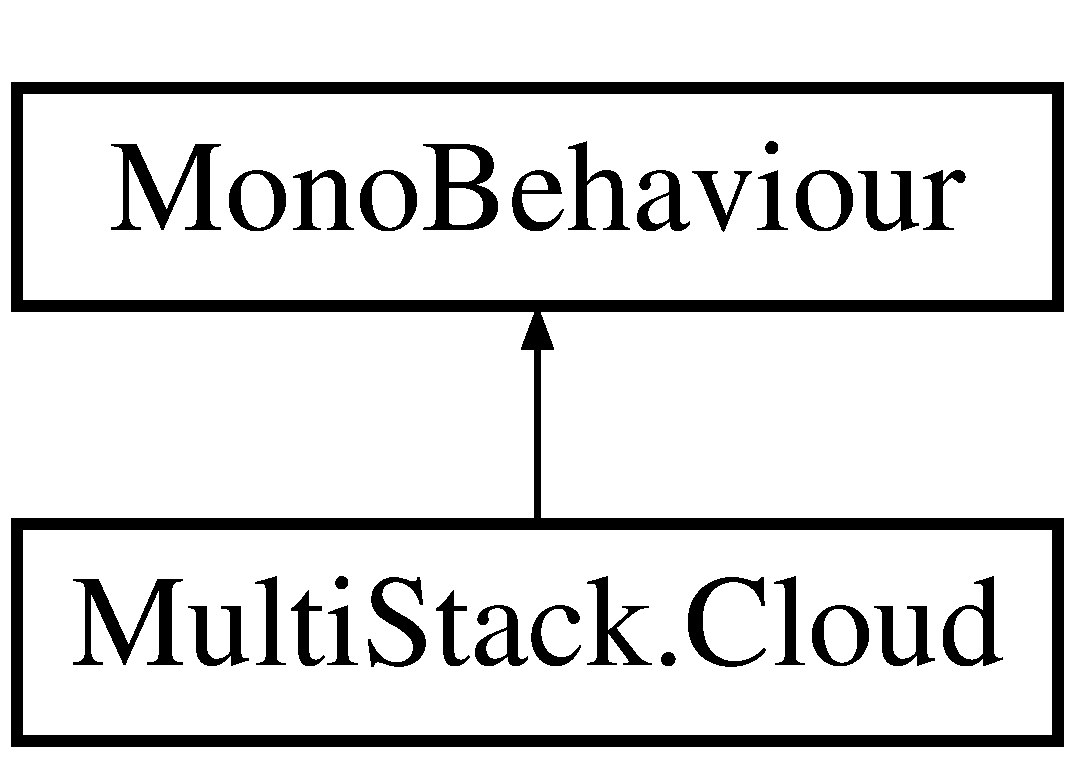
\includegraphics[height=2.000000cm]{class_multi_stack_1_1_cloud}
\end{center}
\end{figure}
\subsection*{Public Attributes}
\begin{DoxyCompactItemize}
\item 
float \hyperlink{class_multi_stack_1_1_cloud_a41c5aba0ae109496d637a7e08c726171}{min\+Speed}
\begin{DoxyCompactList}\small\item\em The minimum speed of the cloud. \end{DoxyCompactList}\item 
float \hyperlink{class_multi_stack_1_1_cloud_ad665595ffaaa5c7b5c6d5a7222d40c89}{max\+Speed}
\begin{DoxyCompactList}\small\item\em The maximum speed of the cloud. \end{DoxyCompactList}\end{DoxyCompactItemize}


\subsection{Detailed Description}
Translates a cloud across the screen based on \hyperlink{class_multi_stack_1_1_cloud_a41c5aba0ae109496d637a7e08c726171}{Multi\+Stack.\+Cloud.\+min\+Speed} and \hyperlink{class_multi_stack_1_1_cloud_ad665595ffaaa5c7b5c6d5a7222d40c89}{Multi\+Stack.\+Cloud.\+max\+Speed}. 



\subsection{Member Data Documentation}
\hypertarget{class_multi_stack_1_1_cloud_ad665595ffaaa5c7b5c6d5a7222d40c89}{}\index{Multi\+Stack\+::\+Cloud@{Multi\+Stack\+::\+Cloud}!max\+Speed@{max\+Speed}}
\index{max\+Speed@{max\+Speed}!Multi\+Stack\+::\+Cloud@{Multi\+Stack\+::\+Cloud}}
\subsubsection[{max\+Speed}]{\setlength{\rightskip}{0pt plus 5cm}float Multi\+Stack.\+Cloud.\+max\+Speed}\label{class_multi_stack_1_1_cloud_ad665595ffaaa5c7b5c6d5a7222d40c89}


The maximum speed of the cloud. 

\hypertarget{class_multi_stack_1_1_cloud_a41c5aba0ae109496d637a7e08c726171}{}\index{Multi\+Stack\+::\+Cloud@{Multi\+Stack\+::\+Cloud}!min\+Speed@{min\+Speed}}
\index{min\+Speed@{min\+Speed}!Multi\+Stack\+::\+Cloud@{Multi\+Stack\+::\+Cloud}}
\subsubsection[{min\+Speed}]{\setlength{\rightskip}{0pt plus 5cm}float Multi\+Stack.\+Cloud.\+min\+Speed}\label{class_multi_stack_1_1_cloud_a41c5aba0ae109496d637a7e08c726171}


The minimum speed of the cloud. 



The documentation for this class was generated from the following file\+:\begin{DoxyCompactItemize}
\item 
Multiplayer\+Stacker/\+Scripts/\+Environment/\+Clouds/Cloud.\+cs\end{DoxyCompactItemize}

\hypertarget{class_multi_stack_1_1_cloud_controller}{}\section{Multi\+Stack.\+Cloud\+Controller Class Reference}
\label{class_multi_stack_1_1_cloud_controller}\index{Multi\+Stack.\+Cloud\+Controller@{Multi\+Stack.\+Cloud\+Controller}}


Handles creation of clouds.  


Inheritance diagram for Multi\+Stack.\+Cloud\+Controller\+:\begin{figure}[H]
\begin{center}
\leavevmode
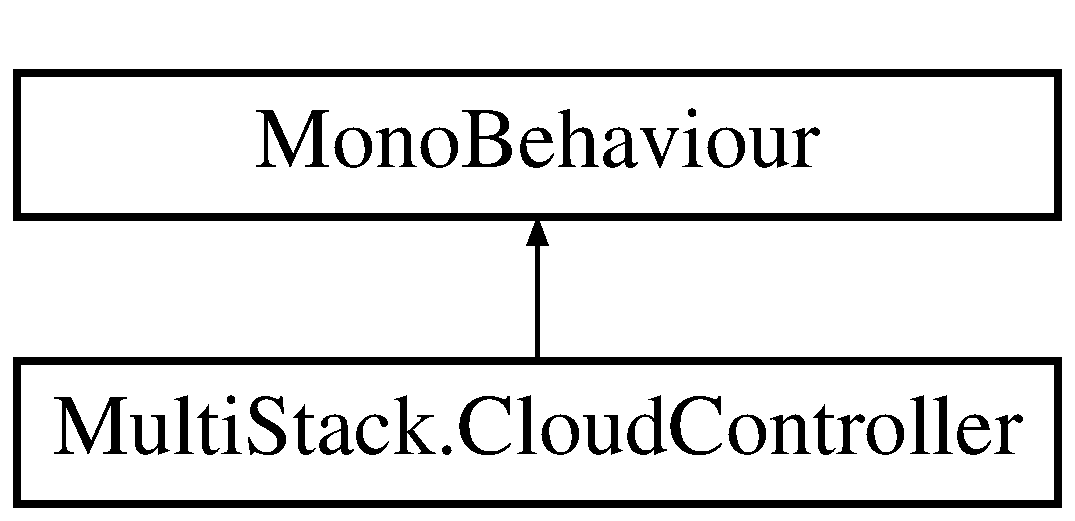
\includegraphics[height=2.000000cm]{class_multi_stack_1_1_cloud_controller}
\end{center}
\end{figure}
\subsection*{Public Member Functions}
\begin{DoxyCompactItemize}
\item 
void \hyperlink{class_multi_stack_1_1_cloud_controller_a10db53c6e52758567af0bcaf8394b43d}{Pool\+Cloud} (Game\+Object cloud)
\begin{DoxyCompactList}\small\item\em Adds a cloud to a pool to be reused when a new cloud is required. \end{DoxyCompactList}\end{DoxyCompactItemize}
\subsection*{Public Attributes}
\begin{DoxyCompactItemize}
\item 
float \hyperlink{class_multi_stack_1_1_cloud_controller_aaa4be94bf648790a61668b77ab5563fd}{max\+Time\+Between\+Clouds}
\begin{DoxyCompactList}\small\item\em The maximum time between spawning clouds. \end{DoxyCompactList}\item 
float \hyperlink{class_multi_stack_1_1_cloud_controller_ab1e3aada1f33156adbdbc3fee236d469}{min\+Time\+Between\+Clouds}
\begin{DoxyCompactList}\small\item\em The minimum time between spawning clouds. \end{DoxyCompactList}\item 
float \hyperlink{class_multi_stack_1_1_cloud_controller_a4315b10736e5440d071a4ffdc67e27fe}{y\+Random\+Offset} = 5f
\begin{DoxyCompactList}\small\item\em A random offset between -\/y\+Random\+Offset and +y\+Random\+Offset is applied to the y position of all spawned clouds. \end{DoxyCompactList}\item 
Game\+Object\mbox{[}$\,$\mbox{]} \hyperlink{class_multi_stack_1_1_cloud_controller_a690f660e3c2720d0bd06174842607783}{cloud\+Prefabs}
\begin{DoxyCompactList}\small\item\em The cloud prefabs to be instantiated. \end{DoxyCompactList}\end{DoxyCompactItemize}


\subsection{Detailed Description}
Handles creation of clouds. 



\subsection{Member Function Documentation}
\hypertarget{class_multi_stack_1_1_cloud_controller_a10db53c6e52758567af0bcaf8394b43d}{}\index{Multi\+Stack\+::\+Cloud\+Controller@{Multi\+Stack\+::\+Cloud\+Controller}!Pool\+Cloud@{Pool\+Cloud}}
\index{Pool\+Cloud@{Pool\+Cloud}!Multi\+Stack\+::\+Cloud\+Controller@{Multi\+Stack\+::\+Cloud\+Controller}}
\subsubsection[{Pool\+Cloud(\+Game\+Object cloud)}]{\setlength{\rightskip}{0pt plus 5cm}void Multi\+Stack.\+Cloud\+Controller.\+Pool\+Cloud (
\begin{DoxyParamCaption}
\item[{Game\+Object}]{cloud}
\end{DoxyParamCaption}
)}\label{class_multi_stack_1_1_cloud_controller_a10db53c6e52758567af0bcaf8394b43d}


Adds a cloud to a pool to be reused when a new cloud is required. 


\begin{DoxyParams}{Parameters}
{\em cloud} & \hyperlink{class_multi_stack_1_1_cloud}{Cloud}.\\
\hline
\end{DoxyParams}


\subsection{Member Data Documentation}
\hypertarget{class_multi_stack_1_1_cloud_controller_a690f660e3c2720d0bd06174842607783}{}\index{Multi\+Stack\+::\+Cloud\+Controller@{Multi\+Stack\+::\+Cloud\+Controller}!cloud\+Prefabs@{cloud\+Prefabs}}
\index{cloud\+Prefabs@{cloud\+Prefabs}!Multi\+Stack\+::\+Cloud\+Controller@{Multi\+Stack\+::\+Cloud\+Controller}}
\subsubsection[{cloud\+Prefabs}]{\setlength{\rightskip}{0pt plus 5cm}Game\+Object \mbox{[}$\,$\mbox{]} Multi\+Stack.\+Cloud\+Controller.\+cloud\+Prefabs}\label{class_multi_stack_1_1_cloud_controller_a690f660e3c2720d0bd06174842607783}


The cloud prefabs to be instantiated. 

\hypertarget{class_multi_stack_1_1_cloud_controller_aaa4be94bf648790a61668b77ab5563fd}{}\index{Multi\+Stack\+::\+Cloud\+Controller@{Multi\+Stack\+::\+Cloud\+Controller}!max\+Time\+Between\+Clouds@{max\+Time\+Between\+Clouds}}
\index{max\+Time\+Between\+Clouds@{max\+Time\+Between\+Clouds}!Multi\+Stack\+::\+Cloud\+Controller@{Multi\+Stack\+::\+Cloud\+Controller}}
\subsubsection[{max\+Time\+Between\+Clouds}]{\setlength{\rightskip}{0pt plus 5cm}float Multi\+Stack.\+Cloud\+Controller.\+max\+Time\+Between\+Clouds}\label{class_multi_stack_1_1_cloud_controller_aaa4be94bf648790a61668b77ab5563fd}


The maximum time between spawning clouds. 

\hypertarget{class_multi_stack_1_1_cloud_controller_ab1e3aada1f33156adbdbc3fee236d469}{}\index{Multi\+Stack\+::\+Cloud\+Controller@{Multi\+Stack\+::\+Cloud\+Controller}!min\+Time\+Between\+Clouds@{min\+Time\+Between\+Clouds}}
\index{min\+Time\+Between\+Clouds@{min\+Time\+Between\+Clouds}!Multi\+Stack\+::\+Cloud\+Controller@{Multi\+Stack\+::\+Cloud\+Controller}}
\subsubsection[{min\+Time\+Between\+Clouds}]{\setlength{\rightskip}{0pt plus 5cm}float Multi\+Stack.\+Cloud\+Controller.\+min\+Time\+Between\+Clouds}\label{class_multi_stack_1_1_cloud_controller_ab1e3aada1f33156adbdbc3fee236d469}


The minimum time between spawning clouds. 

\hypertarget{class_multi_stack_1_1_cloud_controller_a4315b10736e5440d071a4ffdc67e27fe}{}\index{Multi\+Stack\+::\+Cloud\+Controller@{Multi\+Stack\+::\+Cloud\+Controller}!y\+Random\+Offset@{y\+Random\+Offset}}
\index{y\+Random\+Offset@{y\+Random\+Offset}!Multi\+Stack\+::\+Cloud\+Controller@{Multi\+Stack\+::\+Cloud\+Controller}}
\subsubsection[{y\+Random\+Offset}]{\setlength{\rightskip}{0pt plus 5cm}float Multi\+Stack.\+Cloud\+Controller.\+y\+Random\+Offset = 5f}\label{class_multi_stack_1_1_cloud_controller_a4315b10736e5440d071a4ffdc67e27fe}


A random offset between -\/y\+Random\+Offset and +y\+Random\+Offset is applied to the y position of all spawned clouds. 



The documentation for this class was generated from the following file\+:\begin{DoxyCompactItemize}
\item 
Multiplayer\+Stacker/\+Scripts/\+Environment/\+Clouds/Cloud\+Controller.\+cs\end{DoxyCompactItemize}

\hypertarget{class_multi_stack_1_1_cloud_returner}{}\section{Multi\+Stack.\+Cloud\+Returner Class Reference}
\label{class_multi_stack_1_1_cloud_returner}\index{Multi\+Stack.\+Cloud\+Returner@{Multi\+Stack.\+Cloud\+Returner}}


Invokes \hyperlink{class_multi_stack_1_1_cloud_controller_a10db53c6e52758567af0bcaf8394b43d}{Multi\+Stack.\+Cloud\+Controller.\+Pool\+Cloud} when object enters trigger. This is placed at opposite end of the screen to the \hyperlink{class_multi_stack_1_1_cloud_controller}{Multi\+Stack.\+Cloud\+Controller} .  


Inheritance diagram for Multi\+Stack.\+Cloud\+Returner\+:\begin{figure}[H]
\begin{center}
\leavevmode
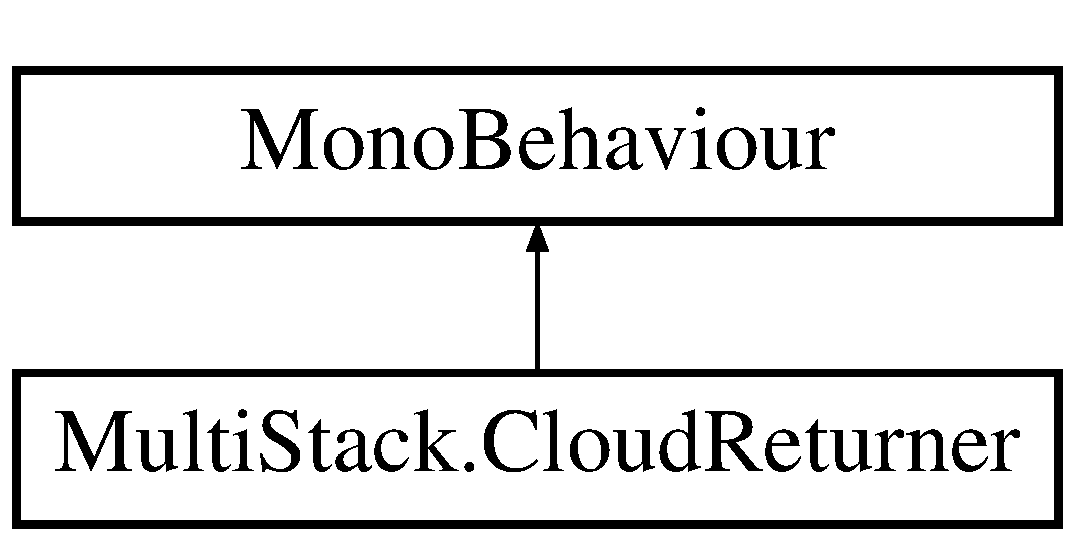
\includegraphics[height=2.000000cm]{class_multi_stack_1_1_cloud_returner}
\end{center}
\end{figure}
\subsection*{Public Attributes}
\begin{DoxyCompactItemize}
\item 
\hyperlink{class_multi_stack_1_1_cloud_controller}{Cloud\+Controller} \hyperlink{class_multi_stack_1_1_cloud_returner_a2a2c664211730eb172f05007161a37e1}{cloud\+Controller}
\begin{DoxyCompactList}\small\item\em Reference to the cloud controller. \end{DoxyCompactList}\end{DoxyCompactItemize}


\subsection{Detailed Description}
Invokes \hyperlink{class_multi_stack_1_1_cloud_controller_a10db53c6e52758567af0bcaf8394b43d}{Multi\+Stack.\+Cloud\+Controller.\+Pool\+Cloud} when object enters trigger. This is placed at opposite end of the screen to the \hyperlink{class_multi_stack_1_1_cloud_controller}{Multi\+Stack.\+Cloud\+Controller} . 



\subsection{Member Data Documentation}
\hypertarget{class_multi_stack_1_1_cloud_returner_a2a2c664211730eb172f05007161a37e1}{}\index{Multi\+Stack\+::\+Cloud\+Returner@{Multi\+Stack\+::\+Cloud\+Returner}!cloud\+Controller@{cloud\+Controller}}
\index{cloud\+Controller@{cloud\+Controller}!Multi\+Stack\+::\+Cloud\+Returner@{Multi\+Stack\+::\+Cloud\+Returner}}
\subsubsection[{cloud\+Controller}]{\setlength{\rightskip}{0pt plus 5cm}{\bf Cloud\+Controller} Multi\+Stack.\+Cloud\+Returner.\+cloud\+Controller}\label{class_multi_stack_1_1_cloud_returner_a2a2c664211730eb172f05007161a37e1}


Reference to the cloud controller. 



The documentation for this class was generated from the following file\+:\begin{DoxyCompactItemize}
\item 
Multiplayer\+Stacker/\+Scripts/\+Environment/\+Clouds/Cloud\+Returner.\+cs\end{DoxyCompactItemize}

\hypertarget{class_multi_stack_1_1_data_persistence}{}\section{Multi\+Stack.\+Data\+Persistence Class Reference}
\label{class_multi_stack_1_1_data_persistence}\index{Multi\+Stack.\+Data\+Persistence@{Multi\+Stack.\+Data\+Persistence}}


Data persistence. Handles saving and loading of height and round data. The highest reached height and round are saved and retrieved from file.  


Inheritance diagram for Multi\+Stack.\+Data\+Persistence\+:\begin{figure}[H]
\begin{center}
\leavevmode
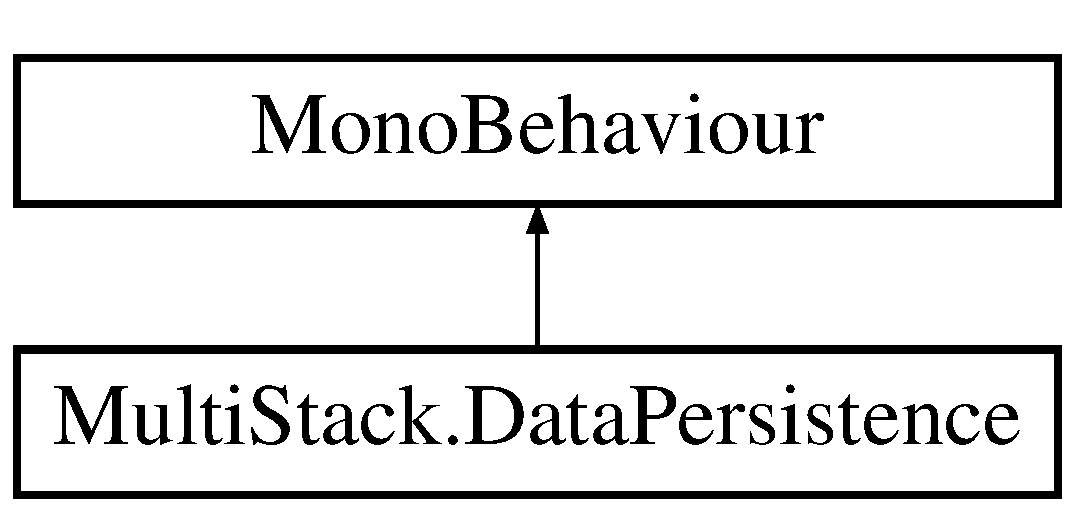
\includegraphics[height=2.000000cm]{class_multi_stack_1_1_data_persistence}
\end{center}
\end{figure}
\subsection*{Public Member Functions}
\begin{DoxyCompactItemize}
\item 
void \hyperlink{class_multi_stack_1_1_data_persistence_a7c9f8ba349cd66a0bc6881fe2d1cc0f7}{Load} ()
\begin{DoxyCompactList}\small\item\em Load the highest round and height from file. \end{DoxyCompactList}\item 
void \hyperlink{class_multi_stack_1_1_data_persistence_a9fc99e077a4fe5b2a49d8508c25d2edd}{Save} (int \hyperlink{class_multi_stack_1_1_data_persistence_af7a5c84c3775aa714c16b32ffc052369}{height}, int \hyperlink{class_multi_stack_1_1_data_persistence_a964cbc11f47af6acf898c8e4d1e3c2fe}{round})
\begin{DoxyCompactList}\small\item\em If height or round score greater than stored height/round then it is saved to file. \end{DoxyCompactList}\end{DoxyCompactItemize}
\subsection*{Properties}
\begin{DoxyCompactItemize}
\item 
int \hyperlink{class_multi_stack_1_1_data_persistence_af7a5c84c3775aa714c16b32ffc052369}{height}\hspace{0.3cm}{\ttfamily  \mbox{[}get\mbox{]}}
\begin{DoxyCompactList}\small\item\em Gets the height. Loaded from file. \end{DoxyCompactList}\item 
int \hyperlink{class_multi_stack_1_1_data_persistence_a964cbc11f47af6acf898c8e4d1e3c2fe}{round}\hspace{0.3cm}{\ttfamily  \mbox{[}get\mbox{]}}
\begin{DoxyCompactList}\small\item\em Gets the round. Loaded from file. \end{DoxyCompactList}\item 
static \hyperlink{class_multi_stack_1_1_data_persistence}{Data\+Persistence} \hyperlink{class_multi_stack_1_1_data_persistence_aa35435eca48c1494a7b196403006da91}{instance}\hspace{0.3cm}{\ttfamily  \mbox{[}get\mbox{]}}
\begin{DoxyCompactList}\small\item\em Gets the instance of this class. Can be accessed from any script. \end{DoxyCompactList}\end{DoxyCompactItemize}


\subsection{Detailed Description}
Data persistence. Handles saving and loading of height and round data. The highest reached height and round are saved and retrieved from file. 



\subsection{Member Function Documentation}
\hypertarget{class_multi_stack_1_1_data_persistence_a7c9f8ba349cd66a0bc6881fe2d1cc0f7}{}\index{Multi\+Stack\+::\+Data\+Persistence@{Multi\+Stack\+::\+Data\+Persistence}!Load@{Load}}
\index{Load@{Load}!Multi\+Stack\+::\+Data\+Persistence@{Multi\+Stack\+::\+Data\+Persistence}}
\subsubsection[{Load()}]{\setlength{\rightskip}{0pt plus 5cm}void Multi\+Stack.\+Data\+Persistence.\+Load (
\begin{DoxyParamCaption}
{}
\end{DoxyParamCaption}
)}\label{class_multi_stack_1_1_data_persistence_a7c9f8ba349cd66a0bc6881fe2d1cc0f7}


Load the highest round and height from file. 

\hypertarget{class_multi_stack_1_1_data_persistence_a9fc99e077a4fe5b2a49d8508c25d2edd}{}\index{Multi\+Stack\+::\+Data\+Persistence@{Multi\+Stack\+::\+Data\+Persistence}!Save@{Save}}
\index{Save@{Save}!Multi\+Stack\+::\+Data\+Persistence@{Multi\+Stack\+::\+Data\+Persistence}}
\subsubsection[{Save(int height, int round)}]{\setlength{\rightskip}{0pt plus 5cm}void Multi\+Stack.\+Data\+Persistence.\+Save (
\begin{DoxyParamCaption}
\item[{int}]{height, }
\item[{int}]{round}
\end{DoxyParamCaption}
)}\label{class_multi_stack_1_1_data_persistence_a9fc99e077a4fe5b2a49d8508c25d2edd}


If height or round score greater than stored height/round then it is saved to file. 


\begin{DoxyParams}{Parameters}
{\em score} & Score.\\
\hline
\end{DoxyParams}


\subsection{Property Documentation}
\hypertarget{class_multi_stack_1_1_data_persistence_af7a5c84c3775aa714c16b32ffc052369}{}\index{Multi\+Stack\+::\+Data\+Persistence@{Multi\+Stack\+::\+Data\+Persistence}!height@{height}}
\index{height@{height}!Multi\+Stack\+::\+Data\+Persistence@{Multi\+Stack\+::\+Data\+Persistence}}
\subsubsection[{height}]{\setlength{\rightskip}{0pt plus 5cm}int Multi\+Stack.\+Data\+Persistence.\+height\hspace{0.3cm}{\ttfamily [get]}}\label{class_multi_stack_1_1_data_persistence_af7a5c84c3775aa714c16b32ffc052369}


Gets the height. Loaded from file. 

The score.\hypertarget{class_multi_stack_1_1_data_persistence_aa35435eca48c1494a7b196403006da91}{}\index{Multi\+Stack\+::\+Data\+Persistence@{Multi\+Stack\+::\+Data\+Persistence}!instance@{instance}}
\index{instance@{instance}!Multi\+Stack\+::\+Data\+Persistence@{Multi\+Stack\+::\+Data\+Persistence}}
\subsubsection[{instance}]{\setlength{\rightskip}{0pt plus 5cm}{\bf Data\+Persistence} Multi\+Stack.\+Data\+Persistence.\+instance\hspace{0.3cm}{\ttfamily [static]}, {\ttfamily [get]}}\label{class_multi_stack_1_1_data_persistence_aa35435eca48c1494a7b196403006da91}


Gets the instance of this class. Can be accessed from any script. 

The instance.\hypertarget{class_multi_stack_1_1_data_persistence_a964cbc11f47af6acf898c8e4d1e3c2fe}{}\index{Multi\+Stack\+::\+Data\+Persistence@{Multi\+Stack\+::\+Data\+Persistence}!round@{round}}
\index{round@{round}!Multi\+Stack\+::\+Data\+Persistence@{Multi\+Stack\+::\+Data\+Persistence}}
\subsubsection[{round}]{\setlength{\rightskip}{0pt plus 5cm}int Multi\+Stack.\+Data\+Persistence.\+round\hspace{0.3cm}{\ttfamily [get]}}\label{class_multi_stack_1_1_data_persistence_a964cbc11f47af6acf898c8e4d1e3c2fe}


Gets the round. Loaded from file. 

The round.

The documentation for this class was generated from the following file\+:\begin{DoxyCompactItemize}
\item 
Multiplayer\+Stacker/\+Scripts/\+High Score/Data\+Persistence.\+cs\end{DoxyCompactItemize}

\hypertarget{class_multi_stack_1_1_destroy}{}\section{Multi\+Stack.\+Destroy Class Reference}
\label{class_multi_stack_1_1_destroy}\index{Multi\+Stack.\+Destroy@{Multi\+Stack.\+Destroy}}


Used during the explosion animation to destroy the gameobject on animation end.  


Inheritance diagram for Multi\+Stack.\+Destroy\+:\begin{figure}[H]
\begin{center}
\leavevmode
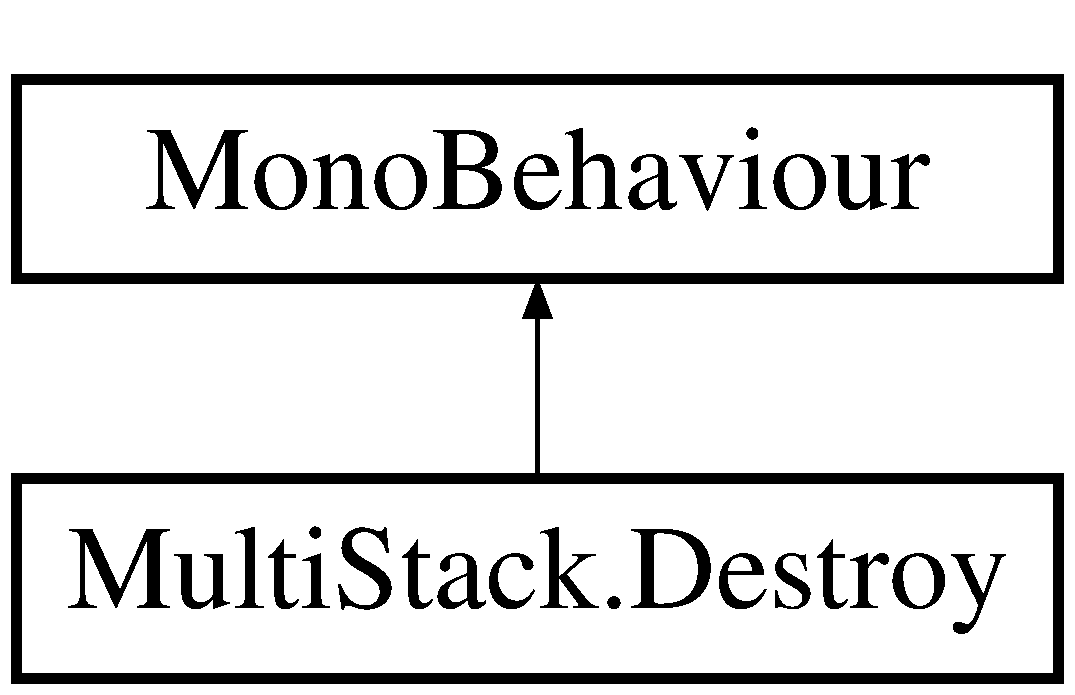
\includegraphics[height=2.000000cm]{class_multi_stack_1_1_destroy}
\end{center}
\end{figure}
\subsection*{Public Member Functions}
\begin{DoxyCompactItemize}
\item 
void \hyperlink{class_multi_stack_1_1_destroy_a9f837df8e5627cc25e3453cc50edad33}{Execute\+Destroy} ()
\begin{DoxyCompactList}\small\item\em Executes the destroy command on gameobject. \end{DoxyCompactList}\end{DoxyCompactItemize}


\subsection{Detailed Description}
Used during the explosion animation to destroy the gameobject on animation end. 



\subsection{Member Function Documentation}
\hypertarget{class_multi_stack_1_1_destroy_a9f837df8e5627cc25e3453cc50edad33}{}\index{Multi\+Stack\+::\+Destroy@{Multi\+Stack\+::\+Destroy}!Execute\+Destroy@{Execute\+Destroy}}
\index{Execute\+Destroy@{Execute\+Destroy}!Multi\+Stack\+::\+Destroy@{Multi\+Stack\+::\+Destroy}}
\subsubsection[{Execute\+Destroy()}]{\setlength{\rightskip}{0pt plus 5cm}void Multi\+Stack.\+Destroy.\+Execute\+Destroy (
\begin{DoxyParamCaption}
{}
\end{DoxyParamCaption}
)}\label{class_multi_stack_1_1_destroy_a9f837df8e5627cc25e3453cc50edad33}


Executes the destroy command on gameobject. 



The documentation for this class was generated from the following file\+:\begin{DoxyCompactItemize}
\item 
Multiplayer\+Stacker/\+Scripts/\+Animation/Destroy.\+cs\end{DoxyCompactItemize}

\hypertarget{class_multi_stack_1_1_explosive_object}{}\section{Multi\+Stack.\+Explosive\+Object Class Reference}
\label{class_multi_stack_1_1_explosive_object}\index{Multi\+Stack.\+Explosive\+Object@{Multi\+Stack.\+Explosive\+Object}}


Attached to any shape that can be turned into an explosive shape. Handles changing a shapes sprite and exploding.  


Inheritance diagram for Multi\+Stack.\+Explosive\+Object\+:\begin{figure}[H]
\begin{center}
\leavevmode
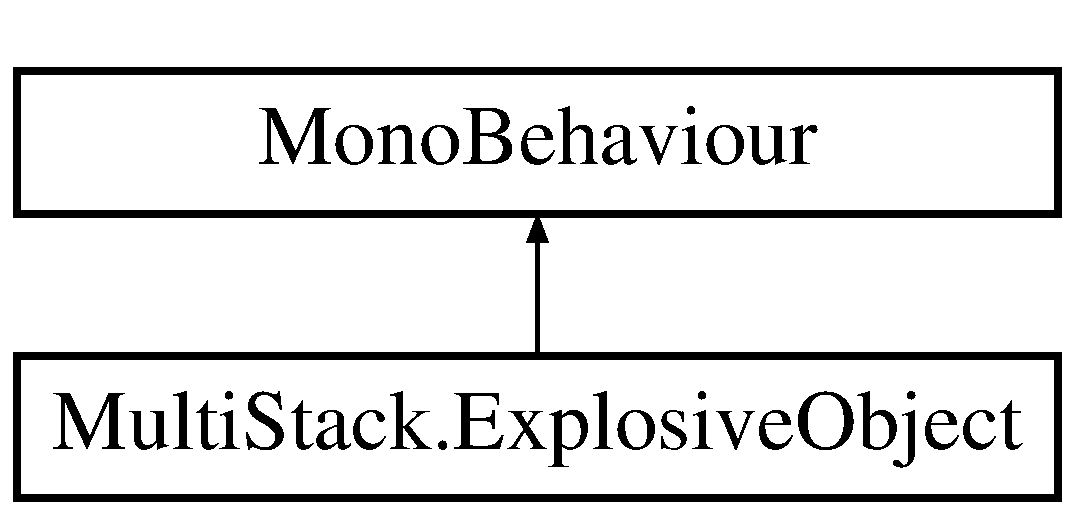
\includegraphics[height=2.000000cm]{class_multi_stack_1_1_explosive_object}
\end{center}
\end{figure}
\subsection*{Public Member Functions}
\begin{DoxyCompactItemize}
\item 
void \hyperlink{class_multi_stack_1_1_explosive_object_a370ff82a75c54370699bf2e6e9a5d3d3}{Activate} ()
\begin{DoxyCompactList}\small\item\em Activate this instance and changes the shapes sprite to that of \hyperlink{class_multi_stack_1_1_explosive_object_a837c3ceaac83c66cbb0b35de25a4821e}{Multi\+Stack.\+Explosive\+Object.\+explosive\+Sprite}. \end{DoxyCompactList}\item 
void \hyperlink{class_multi_stack_1_1_explosive_object_ae36d61db6bdd7744a6a662da354b00e8}{Execute} ()
\begin{DoxyCompactList}\small\item\em Explodes this shape. Plays explosion audio, instantiates explosion fragments, plays explosion animation, applies explosive force to all shapes within the radius, and enables camera shake. \end{DoxyCompactList}\end{DoxyCompactItemize}
\subsection*{Public Attributes}
\begin{DoxyCompactItemize}
\item 
Game\+Object \hyperlink{class_multi_stack_1_1_explosive_object_a22de7a92e4da52f57888874f2d978f56}{explosion\+Prefab}
\begin{DoxyCompactList}\small\item\em The prfab for the explosion animation. \end{DoxyCompactList}\item 
Sprite \hyperlink{class_multi_stack_1_1_explosive_object_a837c3ceaac83c66cbb0b35de25a4821e}{explosive\+Sprite}
\begin{DoxyCompactList}\small\item\em The shapes explosive sprite. \end{DoxyCompactList}\item 
Game\+Object\mbox{[}$\,$\mbox{]} \hyperlink{class_multi_stack_1_1_explosive_object_a675d3ee346269c79e0b60fb0e6eb38b9}{exploded\+Objects}
\begin{DoxyCompactList}\small\item\em Object prefabs to be spawned when the shape is exploded. \end{DoxyCompactList}\item 
float \hyperlink{class_multi_stack_1_1_explosive_object_abd25f5c7fec269baf7f18cafdb9a8f41}{explosive\+Force} = 500f
\begin{DoxyCompactList}\small\item\em The force applied to shapes within the \hyperlink{class_multi_stack_1_1_explosive_object_a409a2b47d8945963839fae41b038e1f5}{Multi\+Stack.\+Explosive\+Object.\+explosive\+Radius} \end{DoxyCompactList}\item 
float \hyperlink{class_multi_stack_1_1_explosive_object_a409a2b47d8945963839fae41b038e1f5}{explosive\+Radius} = 2f
\begin{DoxyCompactList}\small\item\em The explosion radius. Force is applied to all other shapes within this radius. \end{DoxyCompactList}\item 
float \hyperlink{class_multi_stack_1_1_explosive_object_aa56e67200c145c64a54a898e5b060456}{required\+Force\+To\+Explode} = 5.\+3f
\begin{DoxyCompactList}\small\item\em The force if contact between this shape and another shape to trigger the explosion. \end{DoxyCompactList}\item 
Audio\+Clip \hyperlink{class_multi_stack_1_1_explosive_object_ad7c26f2f4ee443b5f18b935a501bc01d}{explosion\+Audio\+Clip}
\begin{DoxyCompactList}\small\item\em An audio clip to play when an explosion occurs. \end{DoxyCompactList}\end{DoxyCompactItemize}
\subsection*{Properties}
\begin{DoxyCompactItemize}
\item 
bool \hyperlink{class_multi_stack_1_1_explosive_object_a0ecb247bb628265fb91df8d2c0b32a72}{ready\+To\+Be\+Activated}\hspace{0.3cm}{\ttfamily  \mbox{[}get\mbox{]}}
\begin{DoxyCompactList}\small\item\em Gets a value indicating whether this \hyperlink{class_multi_stack_1_1_explosive_object}{Multi\+Stack.\+Explosive\+Object} is ready to be activated. \end{DoxyCompactList}\end{DoxyCompactItemize}


\subsection{Detailed Description}
Attached to any shape that can be turned into an explosive shape. Handles changing a shapes sprite and exploding. 



\subsection{Member Function Documentation}
\hypertarget{class_multi_stack_1_1_explosive_object_a370ff82a75c54370699bf2e6e9a5d3d3}{}\index{Multi\+Stack\+::\+Explosive\+Object@{Multi\+Stack\+::\+Explosive\+Object}!Activate@{Activate}}
\index{Activate@{Activate}!Multi\+Stack\+::\+Explosive\+Object@{Multi\+Stack\+::\+Explosive\+Object}}
\subsubsection[{Activate()}]{\setlength{\rightskip}{0pt plus 5cm}void Multi\+Stack.\+Explosive\+Object.\+Activate (
\begin{DoxyParamCaption}
{}
\end{DoxyParamCaption}
)}\label{class_multi_stack_1_1_explosive_object_a370ff82a75c54370699bf2e6e9a5d3d3}


Activate this instance and changes the shapes sprite to that of \hyperlink{class_multi_stack_1_1_explosive_object_a837c3ceaac83c66cbb0b35de25a4821e}{Multi\+Stack.\+Explosive\+Object.\+explosive\+Sprite}. 

\hypertarget{class_multi_stack_1_1_explosive_object_ae36d61db6bdd7744a6a662da354b00e8}{}\index{Multi\+Stack\+::\+Explosive\+Object@{Multi\+Stack\+::\+Explosive\+Object}!Execute@{Execute}}
\index{Execute@{Execute}!Multi\+Stack\+::\+Explosive\+Object@{Multi\+Stack\+::\+Explosive\+Object}}
\subsubsection[{Execute()}]{\setlength{\rightskip}{0pt plus 5cm}void Multi\+Stack.\+Explosive\+Object.\+Execute (
\begin{DoxyParamCaption}
{}
\end{DoxyParamCaption}
)}\label{class_multi_stack_1_1_explosive_object_ae36d61db6bdd7744a6a662da354b00e8}


Explodes this shape. Plays explosion audio, instantiates explosion fragments, plays explosion animation, applies explosive force to all shapes within the radius, and enables camera shake. 



\subsection{Member Data Documentation}
\hypertarget{class_multi_stack_1_1_explosive_object_a675d3ee346269c79e0b60fb0e6eb38b9}{}\index{Multi\+Stack\+::\+Explosive\+Object@{Multi\+Stack\+::\+Explosive\+Object}!exploded\+Objects@{exploded\+Objects}}
\index{exploded\+Objects@{exploded\+Objects}!Multi\+Stack\+::\+Explosive\+Object@{Multi\+Stack\+::\+Explosive\+Object}}
\subsubsection[{exploded\+Objects}]{\setlength{\rightskip}{0pt plus 5cm}Game\+Object \mbox{[}$\,$\mbox{]} Multi\+Stack.\+Explosive\+Object.\+exploded\+Objects}\label{class_multi_stack_1_1_explosive_object_a675d3ee346269c79e0b60fb0e6eb38b9}


Object prefabs to be spawned when the shape is exploded. 

\hypertarget{class_multi_stack_1_1_explosive_object_ad7c26f2f4ee443b5f18b935a501bc01d}{}\index{Multi\+Stack\+::\+Explosive\+Object@{Multi\+Stack\+::\+Explosive\+Object}!explosion\+Audio\+Clip@{explosion\+Audio\+Clip}}
\index{explosion\+Audio\+Clip@{explosion\+Audio\+Clip}!Multi\+Stack\+::\+Explosive\+Object@{Multi\+Stack\+::\+Explosive\+Object}}
\subsubsection[{explosion\+Audio\+Clip}]{\setlength{\rightskip}{0pt plus 5cm}Audio\+Clip Multi\+Stack.\+Explosive\+Object.\+explosion\+Audio\+Clip}\label{class_multi_stack_1_1_explosive_object_ad7c26f2f4ee443b5f18b935a501bc01d}


An audio clip to play when an explosion occurs. 

\hypertarget{class_multi_stack_1_1_explosive_object_a22de7a92e4da52f57888874f2d978f56}{}\index{Multi\+Stack\+::\+Explosive\+Object@{Multi\+Stack\+::\+Explosive\+Object}!explosion\+Prefab@{explosion\+Prefab}}
\index{explosion\+Prefab@{explosion\+Prefab}!Multi\+Stack\+::\+Explosive\+Object@{Multi\+Stack\+::\+Explosive\+Object}}
\subsubsection[{explosion\+Prefab}]{\setlength{\rightskip}{0pt plus 5cm}Game\+Object Multi\+Stack.\+Explosive\+Object.\+explosion\+Prefab}\label{class_multi_stack_1_1_explosive_object_a22de7a92e4da52f57888874f2d978f56}


The prfab for the explosion animation. 

\hypertarget{class_multi_stack_1_1_explosive_object_abd25f5c7fec269baf7f18cafdb9a8f41}{}\index{Multi\+Stack\+::\+Explosive\+Object@{Multi\+Stack\+::\+Explosive\+Object}!explosive\+Force@{explosive\+Force}}
\index{explosive\+Force@{explosive\+Force}!Multi\+Stack\+::\+Explosive\+Object@{Multi\+Stack\+::\+Explosive\+Object}}
\subsubsection[{explosive\+Force}]{\setlength{\rightskip}{0pt plus 5cm}float Multi\+Stack.\+Explosive\+Object.\+explosive\+Force = 500f}\label{class_multi_stack_1_1_explosive_object_abd25f5c7fec269baf7f18cafdb9a8f41}


The force applied to shapes within the \hyperlink{class_multi_stack_1_1_explosive_object_a409a2b47d8945963839fae41b038e1f5}{Multi\+Stack.\+Explosive\+Object.\+explosive\+Radius} 

\hypertarget{class_multi_stack_1_1_explosive_object_a409a2b47d8945963839fae41b038e1f5}{}\index{Multi\+Stack\+::\+Explosive\+Object@{Multi\+Stack\+::\+Explosive\+Object}!explosive\+Radius@{explosive\+Radius}}
\index{explosive\+Radius@{explosive\+Radius}!Multi\+Stack\+::\+Explosive\+Object@{Multi\+Stack\+::\+Explosive\+Object}}
\subsubsection[{explosive\+Radius}]{\setlength{\rightskip}{0pt plus 5cm}float Multi\+Stack.\+Explosive\+Object.\+explosive\+Radius = 2f}\label{class_multi_stack_1_1_explosive_object_a409a2b47d8945963839fae41b038e1f5}


The explosion radius. Force is applied to all other shapes within this radius. 

\hypertarget{class_multi_stack_1_1_explosive_object_a837c3ceaac83c66cbb0b35de25a4821e}{}\index{Multi\+Stack\+::\+Explosive\+Object@{Multi\+Stack\+::\+Explosive\+Object}!explosive\+Sprite@{explosive\+Sprite}}
\index{explosive\+Sprite@{explosive\+Sprite}!Multi\+Stack\+::\+Explosive\+Object@{Multi\+Stack\+::\+Explosive\+Object}}
\subsubsection[{explosive\+Sprite}]{\setlength{\rightskip}{0pt plus 5cm}Sprite Multi\+Stack.\+Explosive\+Object.\+explosive\+Sprite}\label{class_multi_stack_1_1_explosive_object_a837c3ceaac83c66cbb0b35de25a4821e}


The shapes explosive sprite. 

\hypertarget{class_multi_stack_1_1_explosive_object_aa56e67200c145c64a54a898e5b060456}{}\index{Multi\+Stack\+::\+Explosive\+Object@{Multi\+Stack\+::\+Explosive\+Object}!required\+Force\+To\+Explode@{required\+Force\+To\+Explode}}
\index{required\+Force\+To\+Explode@{required\+Force\+To\+Explode}!Multi\+Stack\+::\+Explosive\+Object@{Multi\+Stack\+::\+Explosive\+Object}}
\subsubsection[{required\+Force\+To\+Explode}]{\setlength{\rightskip}{0pt plus 5cm}float Multi\+Stack.\+Explosive\+Object.\+required\+Force\+To\+Explode = 5.\+3f}\label{class_multi_stack_1_1_explosive_object_aa56e67200c145c64a54a898e5b060456}


The force if contact between this shape and another shape to trigger the explosion. 



\subsection{Property Documentation}
\hypertarget{class_multi_stack_1_1_explosive_object_a0ecb247bb628265fb91df8d2c0b32a72}{}\index{Multi\+Stack\+::\+Explosive\+Object@{Multi\+Stack\+::\+Explosive\+Object}!ready\+To\+Be\+Activated@{ready\+To\+Be\+Activated}}
\index{ready\+To\+Be\+Activated@{ready\+To\+Be\+Activated}!Multi\+Stack\+::\+Explosive\+Object@{Multi\+Stack\+::\+Explosive\+Object}}
\subsubsection[{ready\+To\+Be\+Activated}]{\setlength{\rightskip}{0pt plus 5cm}bool Multi\+Stack.\+Explosive\+Object.\+ready\+To\+Be\+Activated\hspace{0.3cm}{\ttfamily [get]}}\label{class_multi_stack_1_1_explosive_object_a0ecb247bb628265fb91df8d2c0b32a72}


Gets a value indicating whether this \hyperlink{class_multi_stack_1_1_explosive_object}{Multi\+Stack.\+Explosive\+Object} is ready to be activated. 

{\ttfamily true} if ready to be activated; otherwise, {\ttfamily false}.

The documentation for this class was generated from the following file\+:\begin{DoxyCompactItemize}
\item 
Multiplayer\+Stacker/\+Scripts/\+Objects/Explosive\+Object.\+cs\end{DoxyCompactItemize}

\hypertarget{class_multi_stack_1_1_explosive_shape_modifier}{}\section{Multi\+Stack.\+Explosive\+Shape\+Modifier Class Reference}
\label{class_multi_stack_1_1_explosive_shape_modifier}\index{Multi\+Stack.\+Explosive\+Shape\+Modifier@{Multi\+Stack.\+Explosive\+Shape\+Modifier}}


When enabled and conditions met a random shape is turned into an explosive shape. Invokes \hyperlink{class_multi_stack_1_1_turn_manager_a4366a75c5431c6d38c2feeb650f07d54}{Multi\+Stack.\+Turn\+Manager.\+Change\+Shape\+To\+Explosive}.  


Inheritance diagram for Multi\+Stack.\+Explosive\+Shape\+Modifier\+:\begin{figure}[H]
\begin{center}
\leavevmode
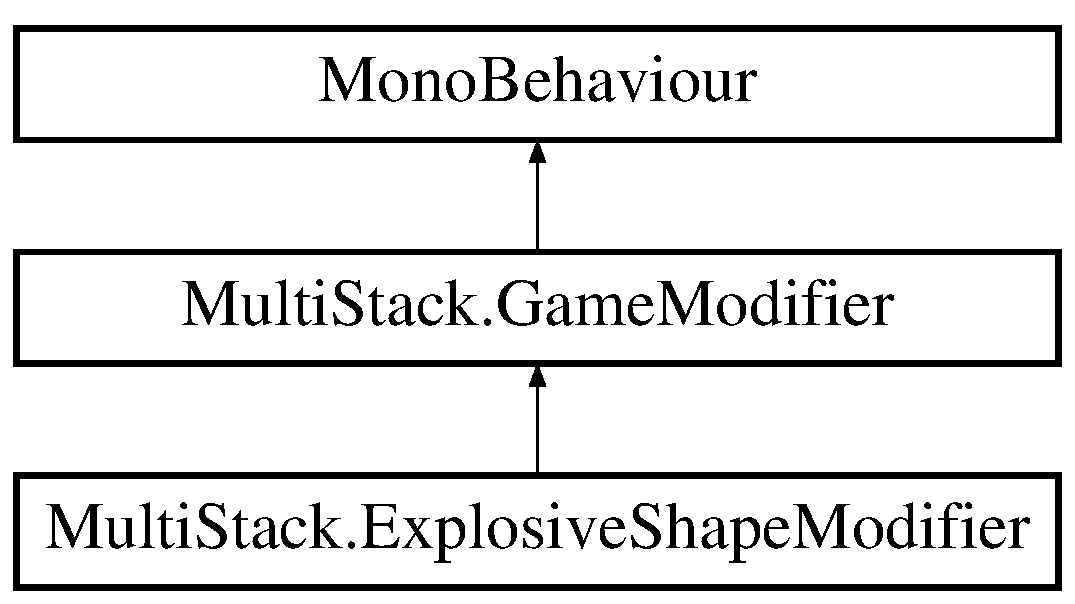
\includegraphics[height=3.000000cm]{class_multi_stack_1_1_explosive_shape_modifier}
\end{center}
\end{figure}
\subsection*{Public Member Functions}
\begin{DoxyCompactItemize}
\item 
override void \hyperlink{class_multi_stack_1_1_explosive_shape_modifier_abf979aeccc0665ec513ab62cb908d981}{Activate} ()
\begin{DoxyCompactList}\small\item\em Activate this modifier. Called at the beginning of the round. \end{DoxyCompactList}\item 
override void \hyperlink{class_multi_stack_1_1_explosive_shape_modifier_a48727a773c318122bc369a48079f2f30}{Deactivate} ()
\begin{DoxyCompactList}\small\item\em Deactivate this modifier. Called before a new modifier is enabled. \end{DoxyCompactList}\item 
override bool \hyperlink{class_multi_stack_1_1_explosive_shape_modifier_adaa2309e63d98090bb81527a3d42d04c}{Conditions\+Met} ()
\begin{DoxyCompactList}\small\item\em Returns true if any spawned shape can be turned into an explosive shape. \end{DoxyCompactList}\end{DoxyCompactItemize}
\subsection*{Additional Inherited Members}


\subsection{Detailed Description}
When enabled and conditions met a random shape is turned into an explosive shape. Invokes \hyperlink{class_multi_stack_1_1_turn_manager_a4366a75c5431c6d38c2feeb650f07d54}{Multi\+Stack.\+Turn\+Manager.\+Change\+Shape\+To\+Explosive}. 



\subsection{Member Function Documentation}
\hypertarget{class_multi_stack_1_1_explosive_shape_modifier_abf979aeccc0665ec513ab62cb908d981}{}\index{Multi\+Stack\+::\+Explosive\+Shape\+Modifier@{Multi\+Stack\+::\+Explosive\+Shape\+Modifier}!Activate@{Activate}}
\index{Activate@{Activate}!Multi\+Stack\+::\+Explosive\+Shape\+Modifier@{Multi\+Stack\+::\+Explosive\+Shape\+Modifier}}
\subsubsection[{Activate()}]{\setlength{\rightskip}{0pt plus 5cm}override void Multi\+Stack.\+Explosive\+Shape\+Modifier.\+Activate (
\begin{DoxyParamCaption}
{}
\end{DoxyParamCaption}
)\hspace{0.3cm}{\ttfamily [virtual]}}\label{class_multi_stack_1_1_explosive_shape_modifier_abf979aeccc0665ec513ab62cb908d981}


Activate this modifier. Called at the beginning of the round. 



Implements \hyperlink{class_multi_stack_1_1_game_modifier_a3fb880f9728f8680bf473ac5c7f6832e}{Multi\+Stack.\+Game\+Modifier}.

\hypertarget{class_multi_stack_1_1_explosive_shape_modifier_adaa2309e63d98090bb81527a3d42d04c}{}\index{Multi\+Stack\+::\+Explosive\+Shape\+Modifier@{Multi\+Stack\+::\+Explosive\+Shape\+Modifier}!Conditions\+Met@{Conditions\+Met}}
\index{Conditions\+Met@{Conditions\+Met}!Multi\+Stack\+::\+Explosive\+Shape\+Modifier@{Multi\+Stack\+::\+Explosive\+Shape\+Modifier}}
\subsubsection[{Conditions\+Met()}]{\setlength{\rightskip}{0pt plus 5cm}override bool Multi\+Stack.\+Explosive\+Shape\+Modifier.\+Conditions\+Met (
\begin{DoxyParamCaption}
{}
\end{DoxyParamCaption}
)\hspace{0.3cm}{\ttfamily [virtual]}}\label{class_multi_stack_1_1_explosive_shape_modifier_adaa2309e63d98090bb81527a3d42d04c}


Returns true if any spawned shape can be turned into an explosive shape. 

\begin{DoxyReturn}{Returns}
true if a shape can be turned into explosive shape.
\end{DoxyReturn}
{\ttfamily false} 

Reimplemented from \hyperlink{class_multi_stack_1_1_game_modifier_acbf45f289c8da7d9aaf129573b2c807c}{Multi\+Stack.\+Game\+Modifier}.

\hypertarget{class_multi_stack_1_1_explosive_shape_modifier_a48727a773c318122bc369a48079f2f30}{}\index{Multi\+Stack\+::\+Explosive\+Shape\+Modifier@{Multi\+Stack\+::\+Explosive\+Shape\+Modifier}!Deactivate@{Deactivate}}
\index{Deactivate@{Deactivate}!Multi\+Stack\+::\+Explosive\+Shape\+Modifier@{Multi\+Stack\+::\+Explosive\+Shape\+Modifier}}
\subsubsection[{Deactivate()}]{\setlength{\rightskip}{0pt plus 5cm}override void Multi\+Stack.\+Explosive\+Shape\+Modifier.\+Deactivate (
\begin{DoxyParamCaption}
{}
\end{DoxyParamCaption}
)\hspace{0.3cm}{\ttfamily [virtual]}}\label{class_multi_stack_1_1_explosive_shape_modifier_a48727a773c318122bc369a48079f2f30}


Deactivate this modifier. Called before a new modifier is enabled. 



Implements \hyperlink{class_multi_stack_1_1_game_modifier_abe04db6ab31f5e5063739d8e5a3f7ad1}{Multi\+Stack.\+Game\+Modifier}.



The documentation for this class was generated from the following file\+:\begin{DoxyCompactItemize}
\item 
Multiplayer\+Stacker/\+Scripts/\+Modifiers/Explosive\+Shape\+Modifier.\+cs\end{DoxyCompactItemize}

\hypertarget{class_multi_stack_1_1_fall_handler}{}\section{Multi\+Stack.\+Fall\+Handler Class Reference}
\label{class_multi_stack_1_1_fall_handler}\index{Multi\+Stack.\+Fall\+Handler@{Multi\+Stack.\+Fall\+Handler}}


Moves camera position to this position if a physics object enters its trigger. Used to move camera to a falling shape.  


Inheritance diagram for Multi\+Stack.\+Fall\+Handler\+:\begin{figure}[H]
\begin{center}
\leavevmode
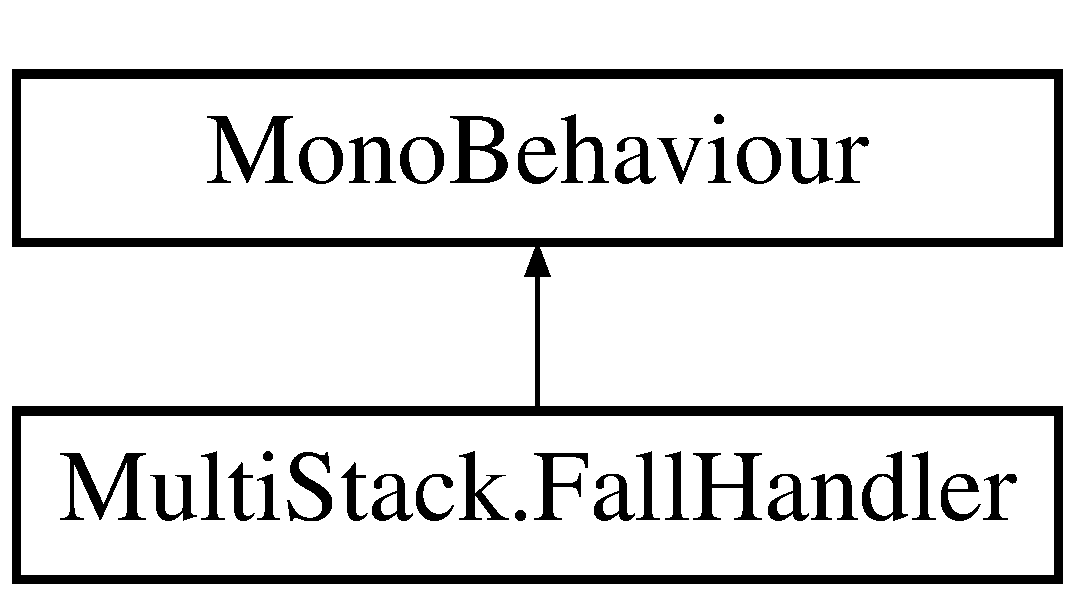
\includegraphics[height=2.000000cm]{class_multi_stack_1_1_fall_handler}
\end{center}
\end{figure}
\subsection*{Public Attributes}
\begin{DoxyCompactItemize}
\item 
Layer\+Mask \hyperlink{class_multi_stack_1_1_fall_handler_ad7f6668311c604a6c8780f43d111b637}{box\+Mask}
\begin{DoxyCompactList}\small\item\em The layermask of the physics object. \end{DoxyCompactList}\item 
float \hyperlink{class_multi_stack_1_1_fall_handler_a29322f628b3b2755771970610f11c382}{required\+Rigid\+Body\+Y\+Velocity} = 4f
\begin{DoxyCompactList}\small\item\em The required physics shape y velocity for the camera to focus on the object. \end{DoxyCompactList}\item 
float \hyperlink{class_multi_stack_1_1_fall_handler_a8bfc0ce850601f85f1d5124f31442bce}{pan\+Speed} = 2f
\begin{DoxyCompactList}\small\item\em The speed at which the camera pans to the object. \end{DoxyCompactList}\end{DoxyCompactItemize}


\subsection{Detailed Description}
Moves camera position to this position if a physics object enters its trigger. Used to move camera to a falling shape. 



\subsection{Member Data Documentation}
\hypertarget{class_multi_stack_1_1_fall_handler_ad7f6668311c604a6c8780f43d111b637}{}\index{Multi\+Stack\+::\+Fall\+Handler@{Multi\+Stack\+::\+Fall\+Handler}!box\+Mask@{box\+Mask}}
\index{box\+Mask@{box\+Mask}!Multi\+Stack\+::\+Fall\+Handler@{Multi\+Stack\+::\+Fall\+Handler}}
\subsubsection[{box\+Mask}]{\setlength{\rightskip}{0pt plus 5cm}Layer\+Mask Multi\+Stack.\+Fall\+Handler.\+box\+Mask}\label{class_multi_stack_1_1_fall_handler_ad7f6668311c604a6c8780f43d111b637}


The layermask of the physics object. 

\hypertarget{class_multi_stack_1_1_fall_handler_a8bfc0ce850601f85f1d5124f31442bce}{}\index{Multi\+Stack\+::\+Fall\+Handler@{Multi\+Stack\+::\+Fall\+Handler}!pan\+Speed@{pan\+Speed}}
\index{pan\+Speed@{pan\+Speed}!Multi\+Stack\+::\+Fall\+Handler@{Multi\+Stack\+::\+Fall\+Handler}}
\subsubsection[{pan\+Speed}]{\setlength{\rightskip}{0pt plus 5cm}float Multi\+Stack.\+Fall\+Handler.\+pan\+Speed = 2f}\label{class_multi_stack_1_1_fall_handler_a8bfc0ce850601f85f1d5124f31442bce}


The speed at which the camera pans to the object. 

\hypertarget{class_multi_stack_1_1_fall_handler_a29322f628b3b2755771970610f11c382}{}\index{Multi\+Stack\+::\+Fall\+Handler@{Multi\+Stack\+::\+Fall\+Handler}!required\+Rigid\+Body\+Y\+Velocity@{required\+Rigid\+Body\+Y\+Velocity}}
\index{required\+Rigid\+Body\+Y\+Velocity@{required\+Rigid\+Body\+Y\+Velocity}!Multi\+Stack\+::\+Fall\+Handler@{Multi\+Stack\+::\+Fall\+Handler}}
\subsubsection[{required\+Rigid\+Body\+Y\+Velocity}]{\setlength{\rightskip}{0pt plus 5cm}float Multi\+Stack.\+Fall\+Handler.\+required\+Rigid\+Body\+Y\+Velocity = 4f}\label{class_multi_stack_1_1_fall_handler_a29322f628b3b2755771970610f11c382}


The required physics shape y velocity for the camera to focus on the object. 



The documentation for this class was generated from the following file\+:\begin{DoxyCompactItemize}
\item 
Multiplayer\+Stacker/\+Scripts/\+Managers/Fall\+Handler.\+cs\end{DoxyCompactItemize}

\hypertarget{class_multi_stack_1_1_game_manager}{}\section{Multi\+Stack.\+Game\+Manager Class Reference}
\label{class_multi_stack_1_1_game_manager}\index{Multi\+Stack.\+Game\+Manager@{Multi\+Stack.\+Game\+Manager}}


Controls the game flow. Handles beginning the game, spawning the stage, starting new rounds, and ending the game.  


Inheritance diagram for Multi\+Stack.\+Game\+Manager\+:\begin{figure}[H]
\begin{center}
\leavevmode
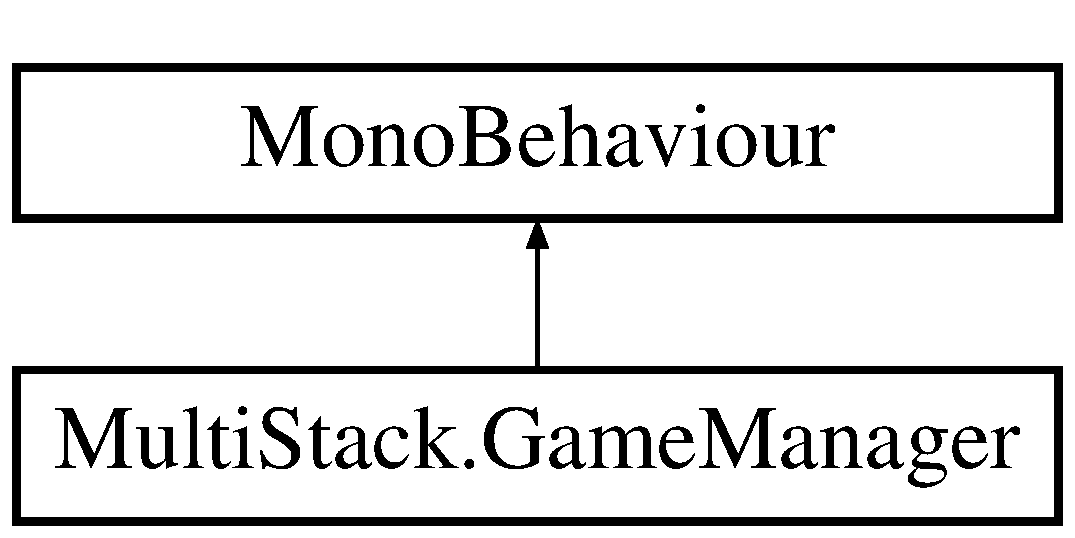
\includegraphics[height=2.000000cm]{class_multi_stack_1_1_game_manager}
\end{center}
\end{figure}
\subsection*{Public Member Functions}
\begin{DoxyCompactItemize}
\item 
void \hyperlink{class_multi_stack_1_1_game_manager_a8c599ec14abfba5712e9631a00d4ec59}{On\+Game\+Over} (\hyperlink{namespace_multi_stack_a19d387de624d6945620427c53c4f0c10}{Game\+Over\+Type} game\+Over\+Type=Game\+Over\+Type.\+Shape\+Off\+Screen)
\begin{DoxyCompactList}\small\item\em Called in the event of a game over (either a players timer reaches zero or a shape falls out of bounds). Disables camera panning and \hyperlink{class_multi_stack_1_1_turn_manager}{Multi\+Stack.\+Turn\+Manager} updates, and saves current height and round via \hyperlink{class_multi_stack_1_1_data_persistence}{Multi\+Stack.\+Data\+Persistence} \end{DoxyCompactList}\item 
void \hyperlink{class_multi_stack_1_1_game_manager_aa8e72d64791c9e4db6815341488110fd}{On\+Round\+Over} ()
\begin{DoxyCompactList}\small\item\em Raised at the end of each round. Shows new round text, applies a round modifier via \hyperlink{class_multi_stack_1_1_game_modifier_manager}{Multi\+Stack.\+Game\+Modifier\+Manager} and invokes \hyperlink{class_multi_stack_1_1_turn_manager_ae7cb8bf242a4c9cc7285be6aa8d3efb8}{Multi\+Stack.\+Turn\+Manager.\+Start\+New\+Round}. \end{DoxyCompactList}\end{DoxyCompactItemize}
\subsection*{Public Attributes}
\begin{DoxyCompactItemize}
\item 
\hyperlink{class_multi_stack_1_1_u_i_flash}{U\+I\+Flash} \hyperlink{class_multi_stack_1_1_game_manager_aa3378e26e4669efb5cc272dfb2c80d6a}{ui\+Flash}
\begin{DoxyCompactList}\small\item\em Reference to \hyperlink{class_multi_stack_1_1_u_i_flash}{U\+I\+Flash}, used to hide the game behind a semi-\/transparent texture on game over. \end{DoxyCompactList}\item 
\hyperlink{class_multi_stack_1_1_game_over_u_i}{Game\+Over\+U\+I} \hyperlink{class_multi_stack_1_1_game_manager_a6b33f48d117d4db0a6873b1028eebb38}{game\+Over\+U\+I}
\begin{DoxyCompactList}\small\item\em The game over U\+I controller. \end{DoxyCompactList}\item 
\hyperlink{class_multi_stack_1_1_stage_selector}{Stage\+Selector} \hyperlink{class_multi_stack_1_1_game_manager_a5a526de2c9547502f5a8613d609624ef}{stage\+Selector}
\begin{DoxyCompactList}\small\item\em The stage selector. Used to spawn the stage at the beginning of the game. \end{DoxyCompactList}\item 
\hyperlink{class_multi_stack_1_1_game_modifier_manager}{Game\+Modifier\+Manager} \hyperlink{class_multi_stack_1_1_game_manager_a252e0694a8be8d574757504fc5549afd}{game\+Modifier\+Manager}
\begin{DoxyCompactList}\small\item\em The game modifier manager. Used to apply a game modifier at the beginning of each round. \end{DoxyCompactList}\item 
\hyperlink{class_multi_stack_1_1_game_text}{Game\+Text} \hyperlink{class_multi_stack_1_1_game_manager_a479c44610a6637e259add0fa0c3128e4}{info\+Text}
\begin{DoxyCompactList}\small\item\em The info text U\+I object. Provides information to the player. \end{DoxyCompactList}\end{DoxyCompactItemize}
\subsection*{Properties}
\begin{DoxyCompactItemize}
\item 
bool \hyperlink{class_multi_stack_1_1_game_manager_afe212dfefd75cfeb1e3fcc817bb92b64}{is\+Game\+Over}\hspace{0.3cm}{\ttfamily  \mbox{[}get\mbox{]}}
\begin{DoxyCompactList}\small\item\em Gets a value indicating whether the game is over. \end{DoxyCompactList}\item 
static \hyperlink{class_multi_stack_1_1_game_manager}{Game\+Manager} \hyperlink{class_multi_stack_1_1_game_manager_a80429580a27850ee0b78b84ec7cb283e}{instance}\hspace{0.3cm}{\ttfamily  \mbox{[}get\mbox{]}}
\begin{DoxyCompactList}\small\item\em Gets the instance of this class. Accessible from any class. \end{DoxyCompactList}\end{DoxyCompactItemize}


\subsection{Detailed Description}
Controls the game flow. Handles beginning the game, spawning the stage, starting new rounds, and ending the game. 



\subsection{Member Function Documentation}
\hypertarget{class_multi_stack_1_1_game_manager_a8c599ec14abfba5712e9631a00d4ec59}{}\index{Multi\+Stack\+::\+Game\+Manager@{Multi\+Stack\+::\+Game\+Manager}!On\+Game\+Over@{On\+Game\+Over}}
\index{On\+Game\+Over@{On\+Game\+Over}!Multi\+Stack\+::\+Game\+Manager@{Multi\+Stack\+::\+Game\+Manager}}
\subsubsection[{On\+Game\+Over(\+Game\+Over\+Type game\+Over\+Type=\+Game\+Over\+Type.\+Shape\+Off\+Screen)}]{\setlength{\rightskip}{0pt plus 5cm}void Multi\+Stack.\+Game\+Manager.\+On\+Game\+Over (
\begin{DoxyParamCaption}
\item[{{\bf Game\+Over\+Type}}]{game\+Over\+Type = {\ttfamily GameOverType.ShapeOffScreen}}
\end{DoxyParamCaption}
)}\label{class_multi_stack_1_1_game_manager_a8c599ec14abfba5712e9631a00d4ec59}


Called in the event of a game over (either a players timer reaches zero or a shape falls out of bounds). Disables camera panning and \hyperlink{class_multi_stack_1_1_turn_manager}{Multi\+Stack.\+Turn\+Manager} updates, and saves current height and round via \hyperlink{class_multi_stack_1_1_data_persistence}{Multi\+Stack.\+Data\+Persistence} 

\hypertarget{class_multi_stack_1_1_game_manager_aa8e72d64791c9e4db6815341488110fd}{}\index{Multi\+Stack\+::\+Game\+Manager@{Multi\+Stack\+::\+Game\+Manager}!On\+Round\+Over@{On\+Round\+Over}}
\index{On\+Round\+Over@{On\+Round\+Over}!Multi\+Stack\+::\+Game\+Manager@{Multi\+Stack\+::\+Game\+Manager}}
\subsubsection[{On\+Round\+Over()}]{\setlength{\rightskip}{0pt plus 5cm}void Multi\+Stack.\+Game\+Manager.\+On\+Round\+Over (
\begin{DoxyParamCaption}
{}
\end{DoxyParamCaption}
)}\label{class_multi_stack_1_1_game_manager_aa8e72d64791c9e4db6815341488110fd}


Raised at the end of each round. Shows new round text, applies a round modifier via \hyperlink{class_multi_stack_1_1_game_modifier_manager}{Multi\+Stack.\+Game\+Modifier\+Manager} and invokes \hyperlink{class_multi_stack_1_1_turn_manager_ae7cb8bf242a4c9cc7285be6aa8d3efb8}{Multi\+Stack.\+Turn\+Manager.\+Start\+New\+Round}. 



\subsection{Member Data Documentation}
\hypertarget{class_multi_stack_1_1_game_manager_a252e0694a8be8d574757504fc5549afd}{}\index{Multi\+Stack\+::\+Game\+Manager@{Multi\+Stack\+::\+Game\+Manager}!game\+Modifier\+Manager@{game\+Modifier\+Manager}}
\index{game\+Modifier\+Manager@{game\+Modifier\+Manager}!Multi\+Stack\+::\+Game\+Manager@{Multi\+Stack\+::\+Game\+Manager}}
\subsubsection[{game\+Modifier\+Manager}]{\setlength{\rightskip}{0pt plus 5cm}{\bf Game\+Modifier\+Manager} Multi\+Stack.\+Game\+Manager.\+game\+Modifier\+Manager}\label{class_multi_stack_1_1_game_manager_a252e0694a8be8d574757504fc5549afd}


The game modifier manager. Used to apply a game modifier at the beginning of each round. 

\hypertarget{class_multi_stack_1_1_game_manager_a6b33f48d117d4db0a6873b1028eebb38}{}\index{Multi\+Stack\+::\+Game\+Manager@{Multi\+Stack\+::\+Game\+Manager}!game\+Over\+U\+I@{game\+Over\+U\+I}}
\index{game\+Over\+U\+I@{game\+Over\+U\+I}!Multi\+Stack\+::\+Game\+Manager@{Multi\+Stack\+::\+Game\+Manager}}
\subsubsection[{game\+Over\+U\+I}]{\setlength{\rightskip}{0pt plus 5cm}{\bf Game\+Over\+U\+I} Multi\+Stack.\+Game\+Manager.\+game\+Over\+U\+I}\label{class_multi_stack_1_1_game_manager_a6b33f48d117d4db0a6873b1028eebb38}


The game over U\+I controller. 

\hypertarget{class_multi_stack_1_1_game_manager_a479c44610a6637e259add0fa0c3128e4}{}\index{Multi\+Stack\+::\+Game\+Manager@{Multi\+Stack\+::\+Game\+Manager}!info\+Text@{info\+Text}}
\index{info\+Text@{info\+Text}!Multi\+Stack\+::\+Game\+Manager@{Multi\+Stack\+::\+Game\+Manager}}
\subsubsection[{info\+Text}]{\setlength{\rightskip}{0pt plus 5cm}{\bf Game\+Text} Multi\+Stack.\+Game\+Manager.\+info\+Text}\label{class_multi_stack_1_1_game_manager_a479c44610a6637e259add0fa0c3128e4}


The info text U\+I object. Provides information to the player. 

\hypertarget{class_multi_stack_1_1_game_manager_a5a526de2c9547502f5a8613d609624ef}{}\index{Multi\+Stack\+::\+Game\+Manager@{Multi\+Stack\+::\+Game\+Manager}!stage\+Selector@{stage\+Selector}}
\index{stage\+Selector@{stage\+Selector}!Multi\+Stack\+::\+Game\+Manager@{Multi\+Stack\+::\+Game\+Manager}}
\subsubsection[{stage\+Selector}]{\setlength{\rightskip}{0pt plus 5cm}{\bf Stage\+Selector} Multi\+Stack.\+Game\+Manager.\+stage\+Selector}\label{class_multi_stack_1_1_game_manager_a5a526de2c9547502f5a8613d609624ef}


The stage selector. Used to spawn the stage at the beginning of the game. 

\hypertarget{class_multi_stack_1_1_game_manager_aa3378e26e4669efb5cc272dfb2c80d6a}{}\index{Multi\+Stack\+::\+Game\+Manager@{Multi\+Stack\+::\+Game\+Manager}!ui\+Flash@{ui\+Flash}}
\index{ui\+Flash@{ui\+Flash}!Multi\+Stack\+::\+Game\+Manager@{Multi\+Stack\+::\+Game\+Manager}}
\subsubsection[{ui\+Flash}]{\setlength{\rightskip}{0pt plus 5cm}{\bf U\+I\+Flash} Multi\+Stack.\+Game\+Manager.\+ui\+Flash}\label{class_multi_stack_1_1_game_manager_aa3378e26e4669efb5cc272dfb2c80d6a}


Reference to \hyperlink{class_multi_stack_1_1_u_i_flash}{U\+I\+Flash}, used to hide the game behind a semi-\/transparent texture on game over. 



\subsection{Property Documentation}
\hypertarget{class_multi_stack_1_1_game_manager_a80429580a27850ee0b78b84ec7cb283e}{}\index{Multi\+Stack\+::\+Game\+Manager@{Multi\+Stack\+::\+Game\+Manager}!instance@{instance}}
\index{instance@{instance}!Multi\+Stack\+::\+Game\+Manager@{Multi\+Stack\+::\+Game\+Manager}}
\subsubsection[{instance}]{\setlength{\rightskip}{0pt plus 5cm}{\bf Game\+Manager} Multi\+Stack.\+Game\+Manager.\+instance\hspace{0.3cm}{\ttfamily [static]}, {\ttfamily [get]}}\label{class_multi_stack_1_1_game_manager_a80429580a27850ee0b78b84ec7cb283e}


Gets the instance of this class. Accessible from any class. 

The instance.\hypertarget{class_multi_stack_1_1_game_manager_afe212dfefd75cfeb1e3fcc817bb92b64}{}\index{Multi\+Stack\+::\+Game\+Manager@{Multi\+Stack\+::\+Game\+Manager}!is\+Game\+Over@{is\+Game\+Over}}
\index{is\+Game\+Over@{is\+Game\+Over}!Multi\+Stack\+::\+Game\+Manager@{Multi\+Stack\+::\+Game\+Manager}}
\subsubsection[{is\+Game\+Over}]{\setlength{\rightskip}{0pt plus 5cm}bool Multi\+Stack.\+Game\+Manager.\+is\+Game\+Over\hspace{0.3cm}{\ttfamily [get]}}\label{class_multi_stack_1_1_game_manager_afe212dfefd75cfeb1e3fcc817bb92b64}


Gets a value indicating whether the game is over. 

{\ttfamily true} if is game over; otherwise, {\ttfamily false}.

The documentation for this class was generated from the following file\+:\begin{DoxyCompactItemize}
\item 
Multiplayer\+Stacker/\+Scripts/\+Managers/Game\+Manager.\+cs\end{DoxyCompactItemize}

\hypertarget{class_multi_stack_1_1_game_modifier}{}\section{Multi\+Stack.\+Game\+Modifier Class Reference}
\label{class_multi_stack_1_1_game_modifier}\index{Multi\+Stack.\+Game\+Modifier@{Multi\+Stack.\+Game\+Modifier}}


The abstract base class for every game modifier. Game modifiers are applied each round to change how the game is played.  


Inheritance diagram for Multi\+Stack.\+Game\+Modifier\+:\begin{figure}[H]
\begin{center}
\leavevmode
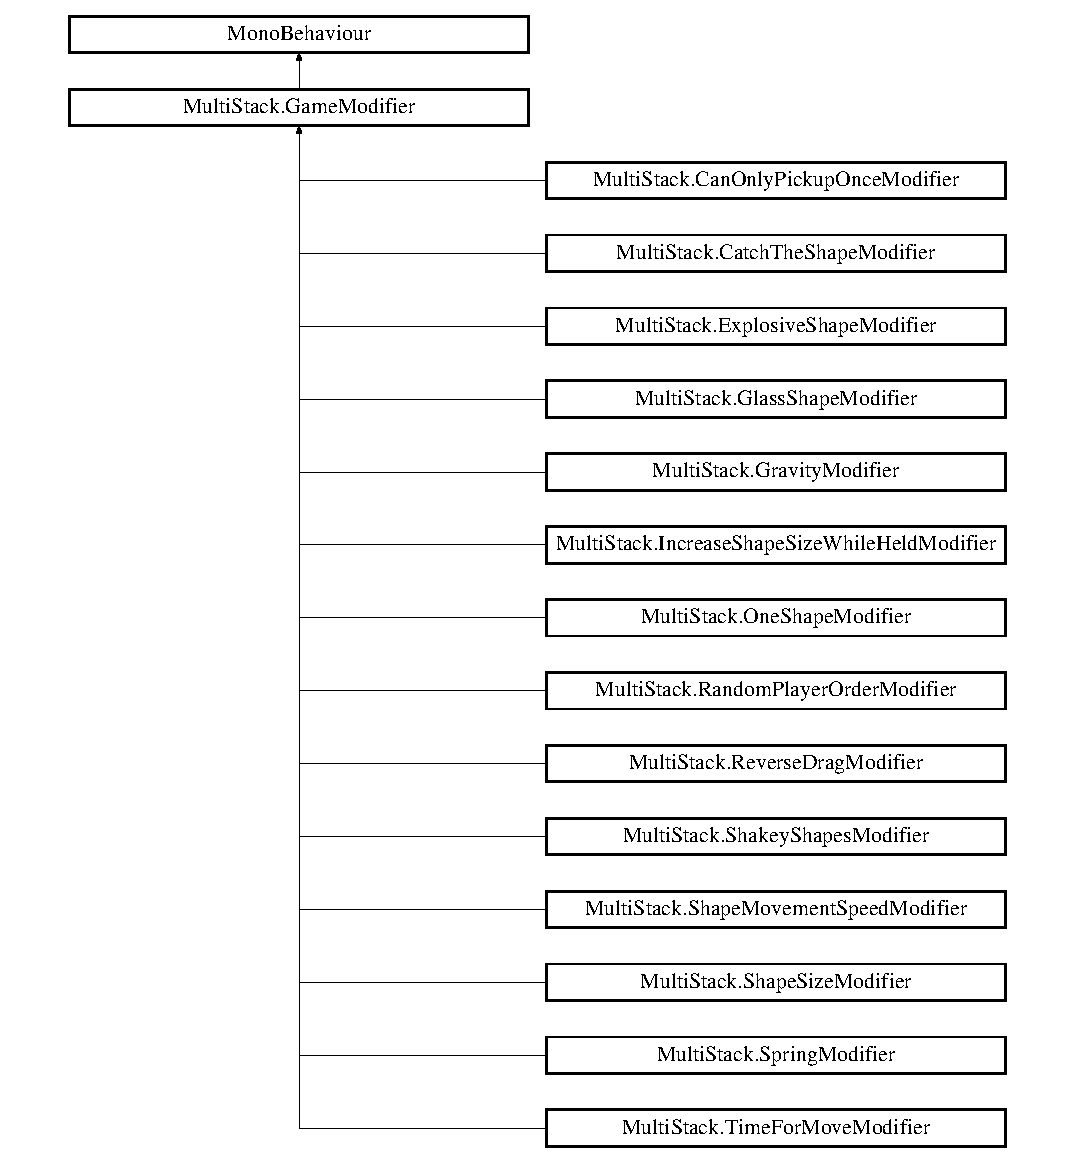
\includegraphics[height=12.000000cm]{class_multi_stack_1_1_game_modifier}
\end{center}
\end{figure}
\subsection*{Public Member Functions}
\begin{DoxyCompactItemize}
\item 
abstract void \hyperlink{class_multi_stack_1_1_game_modifier_a3fb880f9728f8680bf473ac5c7f6832e}{Activate} ()
\begin{DoxyCompactList}\small\item\em Activate this modifier. Called at the beginning of the round. \end{DoxyCompactList}\item 
abstract void \hyperlink{class_multi_stack_1_1_game_modifier_abe04db6ab31f5e5063739d8e5a3f7ad1}{Deactivate} ()
\begin{DoxyCompactList}\small\item\em Deactivate this modifier. Called before a new modifier is enabled. \end{DoxyCompactList}\item 
virtual bool \hyperlink{class_multi_stack_1_1_game_modifier_acbf45f289c8da7d9aaf129573b2c807c}{Conditions\+Met} ()
\begin{DoxyCompactList}\small\item\em Place any prerequisites for the modifier here. By defauly a modifier has all conditions met unless this method is overriden. \end{DoxyCompactList}\end{DoxyCompactItemize}
\subsection*{Public Attributes}
\begin{DoxyCompactItemize}
\item 
bool \hyperlink{class_multi_stack_1_1_game_modifier_a307c902c8fb9fac72d7a4dd74a6bf050}{Is\+Enabled} = true
\begin{DoxyCompactList}\small\item\em Set whether this game modifier is enabled. Disable this in the inspector to prevent the modifier from being applied. \end{DoxyCompactList}\item 
string \hyperlink{class_multi_stack_1_1_game_modifier_ad998250afe8d90cd438b4777a86e34bb}{modifier\+Name}
\begin{DoxyCompactList}\small\item\em The modifier name. This is shown in the U\+I when the modifier is applied. \end{DoxyCompactList}\end{DoxyCompactItemize}


\subsection{Detailed Description}
The abstract base class for every game modifier. Game modifiers are applied each round to change how the game is played. 



\subsection{Member Function Documentation}
\hypertarget{class_multi_stack_1_1_game_modifier_a3fb880f9728f8680bf473ac5c7f6832e}{}\index{Multi\+Stack\+::\+Game\+Modifier@{Multi\+Stack\+::\+Game\+Modifier}!Activate@{Activate}}
\index{Activate@{Activate}!Multi\+Stack\+::\+Game\+Modifier@{Multi\+Stack\+::\+Game\+Modifier}}
\subsubsection[{Activate()}]{\setlength{\rightskip}{0pt plus 5cm}abstract void Multi\+Stack.\+Game\+Modifier.\+Activate (
\begin{DoxyParamCaption}
{}
\end{DoxyParamCaption}
)\hspace{0.3cm}{\ttfamily [pure virtual]}}\label{class_multi_stack_1_1_game_modifier_a3fb880f9728f8680bf473ac5c7f6832e}


Activate this modifier. Called at the beginning of the round. 



Implemented in \hyperlink{class_multi_stack_1_1_one_shape_modifier_a36e475d44744e4f6d5b3dbe1b1ee3a16}{Multi\+Stack.\+One\+Shape\+Modifier}, \hyperlink{class_multi_stack_1_1_time_for_move_modifier_a20bbbf8a51e48116235eff90cfa841a3}{Multi\+Stack.\+Time\+For\+Move\+Modifier}, \hyperlink{class_multi_stack_1_1_gravity_modifier_a752251d8ba8759184857968d2be3327b}{Multi\+Stack.\+Gravity\+Modifier}, \hyperlink{class_multi_stack_1_1_shape_movement_speed_modifier_a9c340894f491f8b11b8753bb4f333d4c}{Multi\+Stack.\+Shape\+Movement\+Speed\+Modifier}, \hyperlink{class_multi_stack_1_1_can_only_pickup_once_modifier_a92da95d7bb53c6c81c60a0a0d28b5c1b}{Multi\+Stack.\+Can\+Only\+Pickup\+Once\+Modifier}, \hyperlink{class_multi_stack_1_1_explosive_shape_modifier_abf979aeccc0665ec513ab62cb908d981}{Multi\+Stack.\+Explosive\+Shape\+Modifier}, \hyperlink{class_multi_stack_1_1_increase_shape_size_while_held_modifier_a85f9b349e3654575248f7d8b4a14868e}{Multi\+Stack.\+Increase\+Shape\+Size\+While\+Held\+Modifier}, \hyperlink{class_multi_stack_1_1_reverse_drag_modifier_a4210fbc0eb598a7b4f31976407e4e1ff}{Multi\+Stack.\+Reverse\+Drag\+Modifier}, \hyperlink{class_multi_stack_1_1_shakey_shapes_modifier_ae45e7bdf85d9655ef28b5a33e0ae72e6}{Multi\+Stack.\+Shakey\+Shapes\+Modifier}, \hyperlink{class_multi_stack_1_1_shape_size_modifier_a5dd27bb25d63f05f2d6c1f4c4f88fd3f}{Multi\+Stack.\+Shape\+Size\+Modifier}, \hyperlink{class_multi_stack_1_1_spring_modifier_ac96460f57d038035461804282c110040}{Multi\+Stack.\+Spring\+Modifier}, \hyperlink{class_multi_stack_1_1_glass_shape_modifier_aeb771b0599250515a886e0175aee746e}{Multi\+Stack.\+Glass\+Shape\+Modifier}, \hyperlink{class_multi_stack_1_1_catch_the_shape_modifier_a5617ebd934298acc024336daa5c633fb}{Multi\+Stack.\+Catch\+The\+Shape\+Modifier}, and \hyperlink{class_multi_stack_1_1_random_player_order_modifier_a6f2965f6ee8933b1631974cefba9bd00}{Multi\+Stack.\+Random\+Player\+Order\+Modifier}.

\hypertarget{class_multi_stack_1_1_game_modifier_acbf45f289c8da7d9aaf129573b2c807c}{}\index{Multi\+Stack\+::\+Game\+Modifier@{Multi\+Stack\+::\+Game\+Modifier}!Conditions\+Met@{Conditions\+Met}}
\index{Conditions\+Met@{Conditions\+Met}!Multi\+Stack\+::\+Game\+Modifier@{Multi\+Stack\+::\+Game\+Modifier}}
\subsubsection[{Conditions\+Met()}]{\setlength{\rightskip}{0pt plus 5cm}virtual bool Multi\+Stack.\+Game\+Modifier.\+Conditions\+Met (
\begin{DoxyParamCaption}
{}
\end{DoxyParamCaption}
)\hspace{0.3cm}{\ttfamily [virtual]}}\label{class_multi_stack_1_1_game_modifier_acbf45f289c8da7d9aaf129573b2c807c}


Place any prerequisites for the modifier here. By defauly a modifier has all conditions met unless this method is overriden. 

\begin{DoxyReturn}{Returns}
{\ttfamily true}, if met was conditionsed, {\ttfamily false} otherwise.
\end{DoxyReturn}


Reimplemented in \hyperlink{class_multi_stack_1_1_explosive_shape_modifier_adaa2309e63d98090bb81527a3d42d04c}{Multi\+Stack.\+Explosive\+Shape\+Modifier}, and \hyperlink{class_multi_stack_1_1_glass_shape_modifier_a75991df9c063e2fc4fd1183001df7206}{Multi\+Stack.\+Glass\+Shape\+Modifier}.

\hypertarget{class_multi_stack_1_1_game_modifier_abe04db6ab31f5e5063739d8e5a3f7ad1}{}\index{Multi\+Stack\+::\+Game\+Modifier@{Multi\+Stack\+::\+Game\+Modifier}!Deactivate@{Deactivate}}
\index{Deactivate@{Deactivate}!Multi\+Stack\+::\+Game\+Modifier@{Multi\+Stack\+::\+Game\+Modifier}}
\subsubsection[{Deactivate()}]{\setlength{\rightskip}{0pt plus 5cm}abstract void Multi\+Stack.\+Game\+Modifier.\+Deactivate (
\begin{DoxyParamCaption}
{}
\end{DoxyParamCaption}
)\hspace{0.3cm}{\ttfamily [pure virtual]}}\label{class_multi_stack_1_1_game_modifier_abe04db6ab31f5e5063739d8e5a3f7ad1}


Deactivate this modifier. Called before a new modifier is enabled. 



Implemented in \hyperlink{class_multi_stack_1_1_one_shape_modifier_a26f5a41e291d04df9a55fd931ff834ec}{Multi\+Stack.\+One\+Shape\+Modifier}, \hyperlink{class_multi_stack_1_1_time_for_move_modifier_a52651c8cbe22e57c0e1d5dd3f4d5fafc}{Multi\+Stack.\+Time\+For\+Move\+Modifier}, \hyperlink{class_multi_stack_1_1_gravity_modifier_a709194d36407f2910ceff941785d8720}{Multi\+Stack.\+Gravity\+Modifier}, \hyperlink{class_multi_stack_1_1_shape_movement_speed_modifier_a6c8209e8db355d3b3204167c76049503}{Multi\+Stack.\+Shape\+Movement\+Speed\+Modifier}, \hyperlink{class_multi_stack_1_1_can_only_pickup_once_modifier_a5375d39256e231f65b9dddc86581b185}{Multi\+Stack.\+Can\+Only\+Pickup\+Once\+Modifier}, \hyperlink{class_multi_stack_1_1_explosive_shape_modifier_a48727a773c318122bc369a48079f2f30}{Multi\+Stack.\+Explosive\+Shape\+Modifier}, \hyperlink{class_multi_stack_1_1_increase_shape_size_while_held_modifier_a936b7d337b1aa5febcfd6eb2ad37a016}{Multi\+Stack.\+Increase\+Shape\+Size\+While\+Held\+Modifier}, \hyperlink{class_multi_stack_1_1_reverse_drag_modifier_a32d5963443ed0867c51c97f76128d3ec}{Multi\+Stack.\+Reverse\+Drag\+Modifier}, \hyperlink{class_multi_stack_1_1_shakey_shapes_modifier_a10f32463b2e5e38d7b50698232e145b4}{Multi\+Stack.\+Shakey\+Shapes\+Modifier}, \hyperlink{class_multi_stack_1_1_shape_size_modifier_a74e6cc4af581e1167679d0b3d9740785}{Multi\+Stack.\+Shape\+Size\+Modifier}, \hyperlink{class_multi_stack_1_1_spring_modifier_ae6aaf8c2806a1c844b1700977efb2dbc}{Multi\+Stack.\+Spring\+Modifier}, \hyperlink{class_multi_stack_1_1_glass_shape_modifier_a44026d971a40d8e5ce02f2611be19b0f}{Multi\+Stack.\+Glass\+Shape\+Modifier}, \hyperlink{class_multi_stack_1_1_catch_the_shape_modifier_ad6ad792bcc0ae5fdd4890af7ec5fe7b1}{Multi\+Stack.\+Catch\+The\+Shape\+Modifier}, and \hyperlink{class_multi_stack_1_1_random_player_order_modifier_a75341a38b55dde95e4037d5ce829ed72}{Multi\+Stack.\+Random\+Player\+Order\+Modifier}.



\subsection{Member Data Documentation}
\hypertarget{class_multi_stack_1_1_game_modifier_a307c902c8fb9fac72d7a4dd74a6bf050}{}\index{Multi\+Stack\+::\+Game\+Modifier@{Multi\+Stack\+::\+Game\+Modifier}!Is\+Enabled@{Is\+Enabled}}
\index{Is\+Enabled@{Is\+Enabled}!Multi\+Stack\+::\+Game\+Modifier@{Multi\+Stack\+::\+Game\+Modifier}}
\subsubsection[{Is\+Enabled}]{\setlength{\rightskip}{0pt plus 5cm}bool Multi\+Stack.\+Game\+Modifier.\+Is\+Enabled = true}\label{class_multi_stack_1_1_game_modifier_a307c902c8fb9fac72d7a4dd74a6bf050}


Set whether this game modifier is enabled. Disable this in the inspector to prevent the modifier from being applied. 

\hypertarget{class_multi_stack_1_1_game_modifier_ad998250afe8d90cd438b4777a86e34bb}{}\index{Multi\+Stack\+::\+Game\+Modifier@{Multi\+Stack\+::\+Game\+Modifier}!modifier\+Name@{modifier\+Name}}
\index{modifier\+Name@{modifier\+Name}!Multi\+Stack\+::\+Game\+Modifier@{Multi\+Stack\+::\+Game\+Modifier}}
\subsubsection[{modifier\+Name}]{\setlength{\rightskip}{0pt plus 5cm}string Multi\+Stack.\+Game\+Modifier.\+modifier\+Name}\label{class_multi_stack_1_1_game_modifier_ad998250afe8d90cd438b4777a86e34bb}


The modifier name. This is shown in the U\+I when the modifier is applied. 



The documentation for this class was generated from the following file\+:\begin{DoxyCompactItemize}
\item 
Multiplayer\+Stacker/\+Scripts/\+Modifiers/Game\+Modifier.\+cs\end{DoxyCompactItemize}

\hypertarget{class_multi_stack_1_1_game_modifier_manager}{}\section{Multi\+Stack.\+Game\+Modifier\+Manager Class Reference}
\label{class_multi_stack_1_1_game_modifier_manager}\index{Multi\+Stack.\+Game\+Modifier\+Manager@{Multi\+Stack.\+Game\+Modifier\+Manager}}


Handles game modifiers. These are modififers applied at the beginning of each round (e.\+g. low gravity).  


Inheritance diagram for Multi\+Stack.\+Game\+Modifier\+Manager\+:\begin{figure}[H]
\begin{center}
\leavevmode
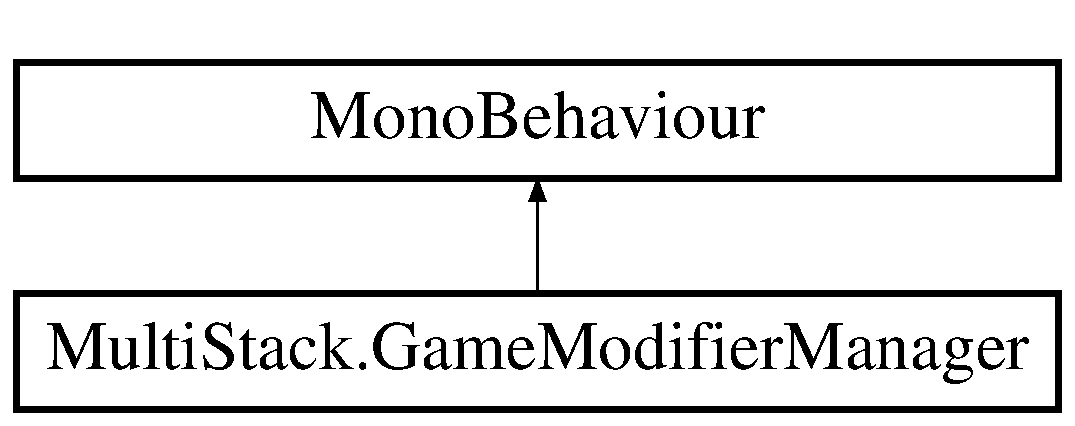
\includegraphics[height=2.000000cm]{class_multi_stack_1_1_game_modifier_manager}
\end{center}
\end{figure}
\subsection*{Public Member Functions}
\begin{DoxyCompactItemize}
\item 
string \hyperlink{class_multi_stack_1_1_game_modifier_manager_a1da0ad850d07870e87f3ab5601e72e05}{Apply\+New\+Modifier} ()
\begin{DoxyCompactList}\small\item\em Applies a new modifier if there are any valid and enabled modifiers. \end{DoxyCompactList}\end{DoxyCompactItemize}


\subsection{Detailed Description}
Handles game modifiers. These are modififers applied at the beginning of each round (e.\+g. low gravity). 



\subsection{Member Function Documentation}
\hypertarget{class_multi_stack_1_1_game_modifier_manager_a1da0ad850d07870e87f3ab5601e72e05}{}\index{Multi\+Stack\+::\+Game\+Modifier\+Manager@{Multi\+Stack\+::\+Game\+Modifier\+Manager}!Apply\+New\+Modifier@{Apply\+New\+Modifier}}
\index{Apply\+New\+Modifier@{Apply\+New\+Modifier}!Multi\+Stack\+::\+Game\+Modifier\+Manager@{Multi\+Stack\+::\+Game\+Modifier\+Manager}}
\subsubsection[{Apply\+New\+Modifier()}]{\setlength{\rightskip}{0pt plus 5cm}string Multi\+Stack.\+Game\+Modifier\+Manager.\+Apply\+New\+Modifier (
\begin{DoxyParamCaption}
{}
\end{DoxyParamCaption}
)}\label{class_multi_stack_1_1_game_modifier_manager_a1da0ad850d07870e87f3ab5601e72e05}


Applies a new modifier if there are any valid and enabled modifiers. 

\begin{DoxyReturn}{Returns}
The new modifiers name, used to update the U\+I.
\end{DoxyReturn}


The documentation for this class was generated from the following file\+:\begin{DoxyCompactItemize}
\item 
Multiplayer\+Stacker/\+Scripts/\+Managers/Game\+Modifier\+Manager.\+cs\end{DoxyCompactItemize}

\hypertarget{class_multi_stack_1_1_game_over_handler}{}\section{Multi\+Stack.\+Game\+Over\+Handler Class Reference}
\label{class_multi_stack_1_1_game_over_handler}\index{Multi\+Stack.\+Game\+Over\+Handler@{Multi\+Stack.\+Game\+Over\+Handler}}


Invokes \hyperlink{class_multi_stack_1_1_game_manager_a8c599ec14abfba5712e9631a00d4ec59}{Multi\+Stack.\+Game\+Manager.\+On\+Game\+Over} when a physics object enters trigger.  


Inheritance diagram for Multi\+Stack.\+Game\+Over\+Handler\+:\begin{figure}[H]
\begin{center}
\leavevmode
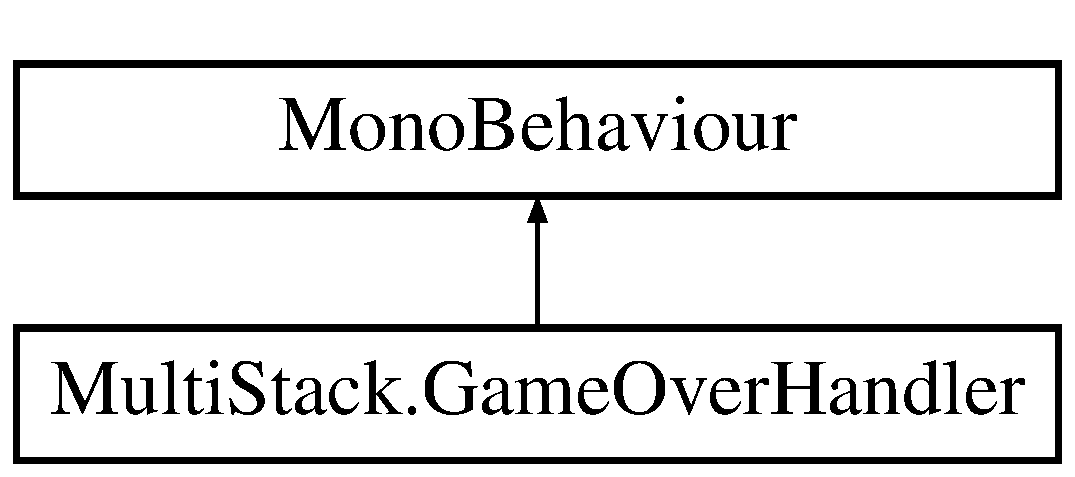
\includegraphics[height=2.000000cm]{class_multi_stack_1_1_game_over_handler}
\end{center}
\end{figure}


\subsection{Detailed Description}
Invokes \hyperlink{class_multi_stack_1_1_game_manager_a8c599ec14abfba5712e9631a00d4ec59}{Multi\+Stack.\+Game\+Manager.\+On\+Game\+Over} when a physics object enters trigger. 



The documentation for this class was generated from the following file\+:\begin{DoxyCompactItemize}
\item 
Multiplayer\+Stacker/\+Scripts/\+Managers/Game\+Over\+Handler.\+cs\end{DoxyCompactItemize}

\hypertarget{class_multi_stack_1_1_game_over_u_i}{}\section{Multi\+Stack.\+Game\+Over\+U\+I Class Reference}
\label{class_multi_stack_1_1_game_over_u_i}\index{Multi\+Stack.\+Game\+Over\+U\+I@{Multi\+Stack.\+Game\+Over\+U\+I}}


Handles the displaying of the U\+I in the event of a game over.  


Inheritance diagram for Multi\+Stack.\+Game\+Over\+U\+I\+:\begin{figure}[H]
\begin{center}
\leavevmode
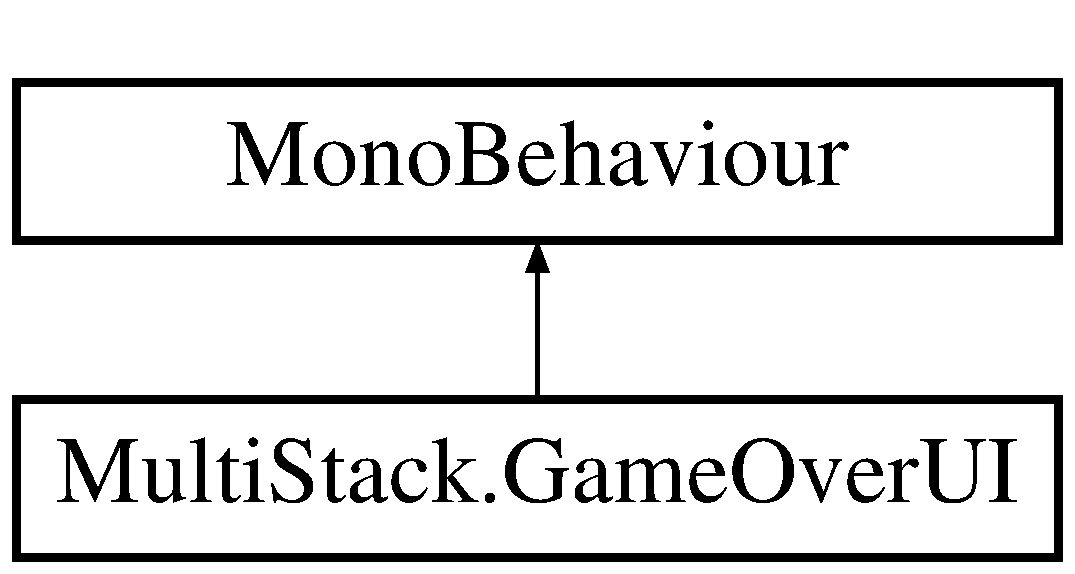
\includegraphics[height=2.000000cm]{class_multi_stack_1_1_game_over_u_i}
\end{center}
\end{figure}
\subsection*{Public Member Functions}
\begin{DoxyCompactItemize}
\item 
void \hyperlink{class_multi_stack_1_1_game_over_u_i_a551012fc4da6e0ab26ec36769f890d3e}{Activate} ()
\begin{DoxyCompactList}\small\item\em Activate this instance. Shows the game over U\+I. \end{DoxyCompactList}\item 
void \hyperlink{class_multi_stack_1_1_game_over_u_i_ab330768d714499d49e51f6a0fa37a828}{Restart\+Scene} ()
\begin{DoxyCompactList}\small\item\em Reloads the current scene. \end{DoxyCompactList}\item 
void \hyperlink{class_multi_stack_1_1_game_over_u_i_a7262bfc9da8aa5c0c48bfc0d2bc6286b}{Return\+To\+Main\+Menu} ()
\begin{DoxyCompactList}\small\item\em Returns to main menu scene. \end{DoxyCompactList}\end{DoxyCompactItemize}
\subsection*{Public Attributes}
\begin{DoxyCompactItemize}
\item 
Game\+Object \hyperlink{class_multi_stack_1_1_game_over_u_i_a05e9dc451638ae9d0a414eb45145f9cc}{title}
\begin{DoxyCompactList}\small\item\em The gameobject for the title U\+I. \end{DoxyCompactList}\item 
Game\+Object \hyperlink{class_multi_stack_1_1_game_over_u_i_ae3084bf607085cbb2cc4d8c4e7897c4b}{new\+Record}
\begin{DoxyCompactList}\small\item\em The gameobject that holds the new record U\+I elements. \end{DoxyCompactList}\item 
\hyperlink{class_multi_stack_1_1_game_text}{Game\+Text}\mbox{[}$\,$\mbox{]} \hyperlink{class_multi_stack_1_1_game_over_u_i_ac8abcfde257e94e4d943e193adff17b9}{non\+Gameover\+U\+I\+Text}
\begin{DoxyCompactList}\small\item\em Add any U\+I not related to the game over U\+I that you would like to hide. \end{DoxyCompactList}\item 
Game\+Object \hyperlink{class_multi_stack_1_1_game_over_u_i_adb0fbbb861cbd3ffe4afee821e549892}{player\+Lost\+Title}
\begin{DoxyCompactList}\small\item\em The title U\+I for player lost. \end{DoxyCompactList}\item 
\hyperlink{class_multi_stack_1_1_game_text}{Game\+Text} \hyperlink{class_multi_stack_1_1_game_over_u_i_a8b3c9a1f48b013cbfb3cc2581e98ba0f}{player\+Lost\+Text}
\begin{DoxyCompactList}\small\item\em The player lost text. Holds the number of the player that has lost the game. \end{DoxyCompactList}\item 
Game\+Object \hyperlink{class_multi_stack_1_1_game_over_u_i_a1d0719d80ce2ba07002511401b65d77c}{height\+Reached\+Title}
\begin{DoxyCompactList}\small\item\em The U\+I title for the hieght field. \end{DoxyCompactList}\item 
\hyperlink{class_multi_stack_1_1_game_text}{Game\+Text} \hyperlink{class_multi_stack_1_1_game_over_u_i_a13eaa345c99a247a23a78f57dc570153}{height\+Reached\+Text}
\begin{DoxyCompactList}\small\item\em The hieght reached text. Holds the height reached the current game. \end{DoxyCompactList}\item 
Game\+Object \hyperlink{class_multi_stack_1_1_game_over_u_i_a4c5b2ff1188a2911cc30e340ef72c66e}{rounds\+Reached\+Title}
\begin{DoxyCompactList}\small\item\em The rounds reached title. \end{DoxyCompactList}\item 
\hyperlink{class_multi_stack_1_1_game_text}{Game\+Text} \hyperlink{class_multi_stack_1_1_game_over_u_i_a0033ad5b25bfd1e023887833069669b9}{rounds\+Reached\+Text}
\begin{DoxyCompactList}\small\item\em The rounds reached text. Holds the round reached in the current game. \end{DoxyCompactList}\item 
Game\+Object \hyperlink{class_multi_stack_1_1_game_over_u_i_a7c0173e7b31a3367c9b75cc1a384c56e}{restart\+Button}
\begin{DoxyCompactList}\small\item\em The restart button. \end{DoxyCompactList}\item 
Game\+Object \hyperlink{class_multi_stack_1_1_game_over_u_i_a4e55a5b8332763f189d1c38877928f5a}{main\+Menu\+Button}
\begin{DoxyCompactList}\small\item\em The main menu button. \end{DoxyCompactList}\end{DoxyCompactItemize}


\subsection{Detailed Description}
Handles the displaying of the U\+I in the event of a game over. 



\subsection{Member Function Documentation}
\hypertarget{class_multi_stack_1_1_game_over_u_i_a551012fc4da6e0ab26ec36769f890d3e}{}\index{Multi\+Stack\+::\+Game\+Over\+U\+I@{Multi\+Stack\+::\+Game\+Over\+U\+I}!Activate@{Activate}}
\index{Activate@{Activate}!Multi\+Stack\+::\+Game\+Over\+U\+I@{Multi\+Stack\+::\+Game\+Over\+U\+I}}
\subsubsection[{Activate()}]{\setlength{\rightskip}{0pt plus 5cm}void Multi\+Stack.\+Game\+Over\+U\+I.\+Activate (
\begin{DoxyParamCaption}
{}
\end{DoxyParamCaption}
)}\label{class_multi_stack_1_1_game_over_u_i_a551012fc4da6e0ab26ec36769f890d3e}


Activate this instance. Shows the game over U\+I. 

\hypertarget{class_multi_stack_1_1_game_over_u_i_ab330768d714499d49e51f6a0fa37a828}{}\index{Multi\+Stack\+::\+Game\+Over\+U\+I@{Multi\+Stack\+::\+Game\+Over\+U\+I}!Restart\+Scene@{Restart\+Scene}}
\index{Restart\+Scene@{Restart\+Scene}!Multi\+Stack\+::\+Game\+Over\+U\+I@{Multi\+Stack\+::\+Game\+Over\+U\+I}}
\subsubsection[{Restart\+Scene()}]{\setlength{\rightskip}{0pt plus 5cm}void Multi\+Stack.\+Game\+Over\+U\+I.\+Restart\+Scene (
\begin{DoxyParamCaption}
{}
\end{DoxyParamCaption}
)}\label{class_multi_stack_1_1_game_over_u_i_ab330768d714499d49e51f6a0fa37a828}


Reloads the current scene. 

\hypertarget{class_multi_stack_1_1_game_over_u_i_a7262bfc9da8aa5c0c48bfc0d2bc6286b}{}\index{Multi\+Stack\+::\+Game\+Over\+U\+I@{Multi\+Stack\+::\+Game\+Over\+U\+I}!Return\+To\+Main\+Menu@{Return\+To\+Main\+Menu}}
\index{Return\+To\+Main\+Menu@{Return\+To\+Main\+Menu}!Multi\+Stack\+::\+Game\+Over\+U\+I@{Multi\+Stack\+::\+Game\+Over\+U\+I}}
\subsubsection[{Return\+To\+Main\+Menu()}]{\setlength{\rightskip}{0pt plus 5cm}void Multi\+Stack.\+Game\+Over\+U\+I.\+Return\+To\+Main\+Menu (
\begin{DoxyParamCaption}
{}
\end{DoxyParamCaption}
)}\label{class_multi_stack_1_1_game_over_u_i_a7262bfc9da8aa5c0c48bfc0d2bc6286b}


Returns to main menu scene. 



\subsection{Member Data Documentation}
\hypertarget{class_multi_stack_1_1_game_over_u_i_a13eaa345c99a247a23a78f57dc570153}{}\index{Multi\+Stack\+::\+Game\+Over\+U\+I@{Multi\+Stack\+::\+Game\+Over\+U\+I}!height\+Reached\+Text@{height\+Reached\+Text}}
\index{height\+Reached\+Text@{height\+Reached\+Text}!Multi\+Stack\+::\+Game\+Over\+U\+I@{Multi\+Stack\+::\+Game\+Over\+U\+I}}
\subsubsection[{height\+Reached\+Text}]{\setlength{\rightskip}{0pt plus 5cm}{\bf Game\+Text} Multi\+Stack.\+Game\+Over\+U\+I.\+height\+Reached\+Text}\label{class_multi_stack_1_1_game_over_u_i_a13eaa345c99a247a23a78f57dc570153}


The hieght reached text. Holds the height reached the current game. 

\hypertarget{class_multi_stack_1_1_game_over_u_i_a1d0719d80ce2ba07002511401b65d77c}{}\index{Multi\+Stack\+::\+Game\+Over\+U\+I@{Multi\+Stack\+::\+Game\+Over\+U\+I}!height\+Reached\+Title@{height\+Reached\+Title}}
\index{height\+Reached\+Title@{height\+Reached\+Title}!Multi\+Stack\+::\+Game\+Over\+U\+I@{Multi\+Stack\+::\+Game\+Over\+U\+I}}
\subsubsection[{height\+Reached\+Title}]{\setlength{\rightskip}{0pt plus 5cm}Game\+Object Multi\+Stack.\+Game\+Over\+U\+I.\+height\+Reached\+Title}\label{class_multi_stack_1_1_game_over_u_i_a1d0719d80ce2ba07002511401b65d77c}


The U\+I title for the hieght field. 

\hypertarget{class_multi_stack_1_1_game_over_u_i_a4e55a5b8332763f189d1c38877928f5a}{}\index{Multi\+Stack\+::\+Game\+Over\+U\+I@{Multi\+Stack\+::\+Game\+Over\+U\+I}!main\+Menu\+Button@{main\+Menu\+Button}}
\index{main\+Menu\+Button@{main\+Menu\+Button}!Multi\+Stack\+::\+Game\+Over\+U\+I@{Multi\+Stack\+::\+Game\+Over\+U\+I}}
\subsubsection[{main\+Menu\+Button}]{\setlength{\rightskip}{0pt plus 5cm}Game\+Object Multi\+Stack.\+Game\+Over\+U\+I.\+main\+Menu\+Button}\label{class_multi_stack_1_1_game_over_u_i_a4e55a5b8332763f189d1c38877928f5a}


The main menu button. 

\hypertarget{class_multi_stack_1_1_game_over_u_i_ae3084bf607085cbb2cc4d8c4e7897c4b}{}\index{Multi\+Stack\+::\+Game\+Over\+U\+I@{Multi\+Stack\+::\+Game\+Over\+U\+I}!new\+Record@{new\+Record}}
\index{new\+Record@{new\+Record}!Multi\+Stack\+::\+Game\+Over\+U\+I@{Multi\+Stack\+::\+Game\+Over\+U\+I}}
\subsubsection[{new\+Record}]{\setlength{\rightskip}{0pt plus 5cm}Game\+Object Multi\+Stack.\+Game\+Over\+U\+I.\+new\+Record}\label{class_multi_stack_1_1_game_over_u_i_ae3084bf607085cbb2cc4d8c4e7897c4b}


The gameobject that holds the new record U\+I elements. 

\hypertarget{class_multi_stack_1_1_game_over_u_i_ac8abcfde257e94e4d943e193adff17b9}{}\index{Multi\+Stack\+::\+Game\+Over\+U\+I@{Multi\+Stack\+::\+Game\+Over\+U\+I}!non\+Gameover\+U\+I\+Text@{non\+Gameover\+U\+I\+Text}}
\index{non\+Gameover\+U\+I\+Text@{non\+Gameover\+U\+I\+Text}!Multi\+Stack\+::\+Game\+Over\+U\+I@{Multi\+Stack\+::\+Game\+Over\+U\+I}}
\subsubsection[{non\+Gameover\+U\+I\+Text}]{\setlength{\rightskip}{0pt plus 5cm}{\bf Game\+Text} \mbox{[}$\,$\mbox{]} Multi\+Stack.\+Game\+Over\+U\+I.\+non\+Gameover\+U\+I\+Text}\label{class_multi_stack_1_1_game_over_u_i_ac8abcfde257e94e4d943e193adff17b9}


Add any U\+I not related to the game over U\+I that you would like to hide. 

\hypertarget{class_multi_stack_1_1_game_over_u_i_a8b3c9a1f48b013cbfb3cc2581e98ba0f}{}\index{Multi\+Stack\+::\+Game\+Over\+U\+I@{Multi\+Stack\+::\+Game\+Over\+U\+I}!player\+Lost\+Text@{player\+Lost\+Text}}
\index{player\+Lost\+Text@{player\+Lost\+Text}!Multi\+Stack\+::\+Game\+Over\+U\+I@{Multi\+Stack\+::\+Game\+Over\+U\+I}}
\subsubsection[{player\+Lost\+Text}]{\setlength{\rightskip}{0pt plus 5cm}{\bf Game\+Text} Multi\+Stack.\+Game\+Over\+U\+I.\+player\+Lost\+Text}\label{class_multi_stack_1_1_game_over_u_i_a8b3c9a1f48b013cbfb3cc2581e98ba0f}


The player lost text. Holds the number of the player that has lost the game. 

\hypertarget{class_multi_stack_1_1_game_over_u_i_adb0fbbb861cbd3ffe4afee821e549892}{}\index{Multi\+Stack\+::\+Game\+Over\+U\+I@{Multi\+Stack\+::\+Game\+Over\+U\+I}!player\+Lost\+Title@{player\+Lost\+Title}}
\index{player\+Lost\+Title@{player\+Lost\+Title}!Multi\+Stack\+::\+Game\+Over\+U\+I@{Multi\+Stack\+::\+Game\+Over\+U\+I}}
\subsubsection[{player\+Lost\+Title}]{\setlength{\rightskip}{0pt plus 5cm}Game\+Object Multi\+Stack.\+Game\+Over\+U\+I.\+player\+Lost\+Title}\label{class_multi_stack_1_1_game_over_u_i_adb0fbbb861cbd3ffe4afee821e549892}


The title U\+I for player lost. 

\hypertarget{class_multi_stack_1_1_game_over_u_i_a7c0173e7b31a3367c9b75cc1a384c56e}{}\index{Multi\+Stack\+::\+Game\+Over\+U\+I@{Multi\+Stack\+::\+Game\+Over\+U\+I}!restart\+Button@{restart\+Button}}
\index{restart\+Button@{restart\+Button}!Multi\+Stack\+::\+Game\+Over\+U\+I@{Multi\+Stack\+::\+Game\+Over\+U\+I}}
\subsubsection[{restart\+Button}]{\setlength{\rightskip}{0pt plus 5cm}Game\+Object Multi\+Stack.\+Game\+Over\+U\+I.\+restart\+Button}\label{class_multi_stack_1_1_game_over_u_i_a7c0173e7b31a3367c9b75cc1a384c56e}


The restart button. 

\hypertarget{class_multi_stack_1_1_game_over_u_i_a0033ad5b25bfd1e023887833069669b9}{}\index{Multi\+Stack\+::\+Game\+Over\+U\+I@{Multi\+Stack\+::\+Game\+Over\+U\+I}!rounds\+Reached\+Text@{rounds\+Reached\+Text}}
\index{rounds\+Reached\+Text@{rounds\+Reached\+Text}!Multi\+Stack\+::\+Game\+Over\+U\+I@{Multi\+Stack\+::\+Game\+Over\+U\+I}}
\subsubsection[{rounds\+Reached\+Text}]{\setlength{\rightskip}{0pt plus 5cm}{\bf Game\+Text} Multi\+Stack.\+Game\+Over\+U\+I.\+rounds\+Reached\+Text}\label{class_multi_stack_1_1_game_over_u_i_a0033ad5b25bfd1e023887833069669b9}


The rounds reached text. Holds the round reached in the current game. 

\hypertarget{class_multi_stack_1_1_game_over_u_i_a4c5b2ff1188a2911cc30e340ef72c66e}{}\index{Multi\+Stack\+::\+Game\+Over\+U\+I@{Multi\+Stack\+::\+Game\+Over\+U\+I}!rounds\+Reached\+Title@{rounds\+Reached\+Title}}
\index{rounds\+Reached\+Title@{rounds\+Reached\+Title}!Multi\+Stack\+::\+Game\+Over\+U\+I@{Multi\+Stack\+::\+Game\+Over\+U\+I}}
\subsubsection[{rounds\+Reached\+Title}]{\setlength{\rightskip}{0pt plus 5cm}Game\+Object Multi\+Stack.\+Game\+Over\+U\+I.\+rounds\+Reached\+Title}\label{class_multi_stack_1_1_game_over_u_i_a4c5b2ff1188a2911cc30e340ef72c66e}


The rounds reached title. 

\hypertarget{class_multi_stack_1_1_game_over_u_i_a05e9dc451638ae9d0a414eb45145f9cc}{}\index{Multi\+Stack\+::\+Game\+Over\+U\+I@{Multi\+Stack\+::\+Game\+Over\+U\+I}!title@{title}}
\index{title@{title}!Multi\+Stack\+::\+Game\+Over\+U\+I@{Multi\+Stack\+::\+Game\+Over\+U\+I}}
\subsubsection[{title}]{\setlength{\rightskip}{0pt plus 5cm}Game\+Object Multi\+Stack.\+Game\+Over\+U\+I.\+title}\label{class_multi_stack_1_1_game_over_u_i_a05e9dc451638ae9d0a414eb45145f9cc}


The gameobject for the title U\+I. 



The documentation for this class was generated from the following file\+:\begin{DoxyCompactItemize}
\item 
Multiplayer\+Stacker/\+Scripts/\+U\+I/Game\+Over\+U\+I.\+cs\end{DoxyCompactItemize}

\hypertarget{class_multi_stack_1_1_game_text}{}\section{Multi\+Stack.\+Game\+Text Class Reference}
\label{class_multi_stack_1_1_game_text}\index{Multi\+Stack.\+Game\+Text@{Multi\+Stack.\+Game\+Text}}


A simple wrapper for the text object.  


Inheritance diagram for Multi\+Stack.\+Game\+Text\+:\begin{figure}[H]
\begin{center}
\leavevmode
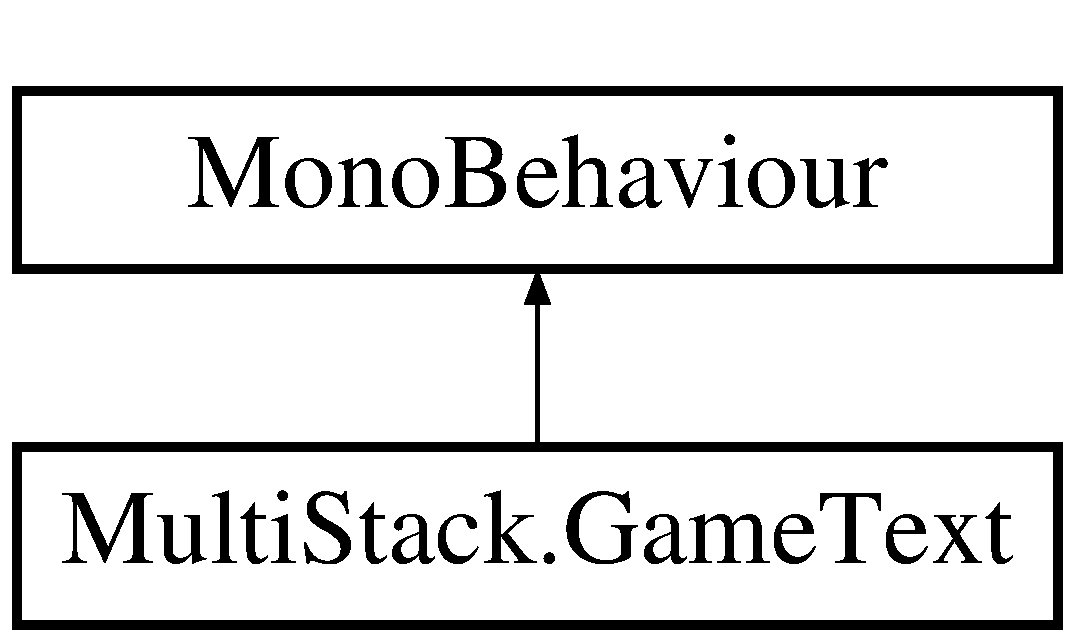
\includegraphics[height=2.000000cm]{class_multi_stack_1_1_game_text}
\end{center}
\end{figure}
\subsection*{Public Member Functions}
\begin{DoxyCompactItemize}
\item 
void \hyperlink{class_multi_stack_1_1_game_text_a55d38f6e4dcfd4b825736558fa3aee5a}{Update\+Text} (string msg, Color colour)
\begin{DoxyCompactList}\small\item\em Updates the U\+I text with the desired font colour. \end{DoxyCompactList}\item 
void \hyperlink{class_multi_stack_1_1_game_text_a1f24ea6be9b694bb21784e27a948820e}{Update\+Text} (string msg)
\begin{DoxyCompactList}\small\item\em Updates the U\+I text. \end{DoxyCompactList}\item 
void \hyperlink{class_multi_stack_1_1_game_text_ad46f062ce89b4a4b05d885c70fbbaf48}{Hide\+Text\+After\+Time} (float seconds)
\begin{DoxyCompactList}\small\item\em Hides the text after time in seconds. \end{DoxyCompactList}\item 
void \hyperlink{class_multi_stack_1_1_game_text_a332f9a4e01cc978cf7e48127a04f9229}{Hide\+Text} ()
\begin{DoxyCompactList}\small\item\em Clears the U\+I text field. \end{DoxyCompactList}\item 
void \hyperlink{class_multi_stack_1_1_game_text_a603da38f9257d8fbc18e033d5cdddf2b}{Change\+Font\+Colour} (Color colour)
\begin{DoxyCompactList}\small\item\em Changes the font colour. \end{DoxyCompactList}\end{DoxyCompactItemize}
\subsection*{Public Attributes}
\begin{DoxyCompactItemize}
\item 
bool \hyperlink{class_multi_stack_1_1_game_text_aad503e1eab16a1649865c8ce4dfa2d7c}{clear\+On\+Start} = true
\begin{DoxyCompactList}\small\item\em C\+Lears all text on scene start. \end{DoxyCompactList}\end{DoxyCompactItemize}
\subsection*{Properties}
\begin{DoxyCompactItemize}
\item 
string \hyperlink{class_multi_stack_1_1_game_text_a0273e94b02ce232e97172bcc27e1e464}{text}\hspace{0.3cm}{\ttfamily  \mbox{[}get\mbox{]}}
\begin{DoxyCompactList}\small\item\em Gets the text value. \end{DoxyCompactList}\end{DoxyCompactItemize}


\subsection{Detailed Description}
A simple wrapper for the text object. 



\subsection{Member Function Documentation}
\hypertarget{class_multi_stack_1_1_game_text_a603da38f9257d8fbc18e033d5cdddf2b}{}\index{Multi\+Stack\+::\+Game\+Text@{Multi\+Stack\+::\+Game\+Text}!Change\+Font\+Colour@{Change\+Font\+Colour}}
\index{Change\+Font\+Colour@{Change\+Font\+Colour}!Multi\+Stack\+::\+Game\+Text@{Multi\+Stack\+::\+Game\+Text}}
\subsubsection[{Change\+Font\+Colour(\+Color colour)}]{\setlength{\rightskip}{0pt plus 5cm}void Multi\+Stack.\+Game\+Text.\+Change\+Font\+Colour (
\begin{DoxyParamCaption}
\item[{Color}]{colour}
\end{DoxyParamCaption}
)}\label{class_multi_stack_1_1_game_text_a603da38f9257d8fbc18e033d5cdddf2b}


Changes the font colour. 


\begin{DoxyParams}{Parameters}
{\em colour} & Colour.\\
\hline
\end{DoxyParams}
\hypertarget{class_multi_stack_1_1_game_text_a332f9a4e01cc978cf7e48127a04f9229}{}\index{Multi\+Stack\+::\+Game\+Text@{Multi\+Stack\+::\+Game\+Text}!Hide\+Text@{Hide\+Text}}
\index{Hide\+Text@{Hide\+Text}!Multi\+Stack\+::\+Game\+Text@{Multi\+Stack\+::\+Game\+Text}}
\subsubsection[{Hide\+Text()}]{\setlength{\rightskip}{0pt plus 5cm}void Multi\+Stack.\+Game\+Text.\+Hide\+Text (
\begin{DoxyParamCaption}
{}
\end{DoxyParamCaption}
)}\label{class_multi_stack_1_1_game_text_a332f9a4e01cc978cf7e48127a04f9229}


Clears the U\+I text field. 

\hypertarget{class_multi_stack_1_1_game_text_ad46f062ce89b4a4b05d885c70fbbaf48}{}\index{Multi\+Stack\+::\+Game\+Text@{Multi\+Stack\+::\+Game\+Text}!Hide\+Text\+After\+Time@{Hide\+Text\+After\+Time}}
\index{Hide\+Text\+After\+Time@{Hide\+Text\+After\+Time}!Multi\+Stack\+::\+Game\+Text@{Multi\+Stack\+::\+Game\+Text}}
\subsubsection[{Hide\+Text\+After\+Time(float seconds)}]{\setlength{\rightskip}{0pt plus 5cm}void Multi\+Stack.\+Game\+Text.\+Hide\+Text\+After\+Time (
\begin{DoxyParamCaption}
\item[{float}]{seconds}
\end{DoxyParamCaption}
)}\label{class_multi_stack_1_1_game_text_ad46f062ce89b4a4b05d885c70fbbaf48}


Hides the text after time in seconds. 


\begin{DoxyParams}{Parameters}
{\em seconds} & Seconds.\\
\hline
\end{DoxyParams}
\hypertarget{class_multi_stack_1_1_game_text_a55d38f6e4dcfd4b825736558fa3aee5a}{}\index{Multi\+Stack\+::\+Game\+Text@{Multi\+Stack\+::\+Game\+Text}!Update\+Text@{Update\+Text}}
\index{Update\+Text@{Update\+Text}!Multi\+Stack\+::\+Game\+Text@{Multi\+Stack\+::\+Game\+Text}}
\subsubsection[{Update\+Text(string msg, Color colour)}]{\setlength{\rightskip}{0pt plus 5cm}void Multi\+Stack.\+Game\+Text.\+Update\+Text (
\begin{DoxyParamCaption}
\item[{string}]{msg, }
\item[{Color}]{colour}
\end{DoxyParamCaption}
)}\label{class_multi_stack_1_1_game_text_a55d38f6e4dcfd4b825736558fa3aee5a}


Updates the U\+I text with the desired font colour. 


\begin{DoxyParams}{Parameters}
{\em msg} & Message.\\
\hline
{\em colour} & Colour.\\
\hline
\end{DoxyParams}
\hypertarget{class_multi_stack_1_1_game_text_a1f24ea6be9b694bb21784e27a948820e}{}\index{Multi\+Stack\+::\+Game\+Text@{Multi\+Stack\+::\+Game\+Text}!Update\+Text@{Update\+Text}}
\index{Update\+Text@{Update\+Text}!Multi\+Stack\+::\+Game\+Text@{Multi\+Stack\+::\+Game\+Text}}
\subsubsection[{Update\+Text(string msg)}]{\setlength{\rightskip}{0pt plus 5cm}void Multi\+Stack.\+Game\+Text.\+Update\+Text (
\begin{DoxyParamCaption}
\item[{string}]{msg}
\end{DoxyParamCaption}
)}\label{class_multi_stack_1_1_game_text_a1f24ea6be9b694bb21784e27a948820e}


Updates the U\+I text. 


\begin{DoxyParams}{Parameters}
{\em msg} & Message.\\
\hline
\end{DoxyParams}


\subsection{Member Data Documentation}
\hypertarget{class_multi_stack_1_1_game_text_aad503e1eab16a1649865c8ce4dfa2d7c}{}\index{Multi\+Stack\+::\+Game\+Text@{Multi\+Stack\+::\+Game\+Text}!clear\+On\+Start@{clear\+On\+Start}}
\index{clear\+On\+Start@{clear\+On\+Start}!Multi\+Stack\+::\+Game\+Text@{Multi\+Stack\+::\+Game\+Text}}
\subsubsection[{clear\+On\+Start}]{\setlength{\rightskip}{0pt plus 5cm}bool Multi\+Stack.\+Game\+Text.\+clear\+On\+Start = true}\label{class_multi_stack_1_1_game_text_aad503e1eab16a1649865c8ce4dfa2d7c}


C\+Lears all text on scene start. 



\subsection{Property Documentation}
\hypertarget{class_multi_stack_1_1_game_text_a0273e94b02ce232e97172bcc27e1e464}{}\index{Multi\+Stack\+::\+Game\+Text@{Multi\+Stack\+::\+Game\+Text}!text@{text}}
\index{text@{text}!Multi\+Stack\+::\+Game\+Text@{Multi\+Stack\+::\+Game\+Text}}
\subsubsection[{text}]{\setlength{\rightskip}{0pt plus 5cm}string Multi\+Stack.\+Game\+Text.\+text\hspace{0.3cm}{\ttfamily [get]}}\label{class_multi_stack_1_1_game_text_a0273e94b02ce232e97172bcc27e1e464}


Gets the text value. 

The text.

The documentation for this class was generated from the following file\+:\begin{DoxyCompactItemize}
\item 
Multiplayer\+Stacker/\+Scripts/\+U\+I/Game\+Text.\+cs\end{DoxyCompactItemize}

\hypertarget{class_multi_stack_1_1_glass_object}{}\section{Multi\+Stack.\+Glass\+Object Class Reference}
\label{class_multi_stack_1_1_glass_object}\index{Multi\+Stack.\+Glass\+Object@{Multi\+Stack.\+Glass\+Object}}


Attached to any shape that can be turned into a glass shape. Handles changing a shapes sprite and breaking.  


Inheritance diagram for Multi\+Stack.\+Glass\+Object\+:\begin{figure}[H]
\begin{center}
\leavevmode
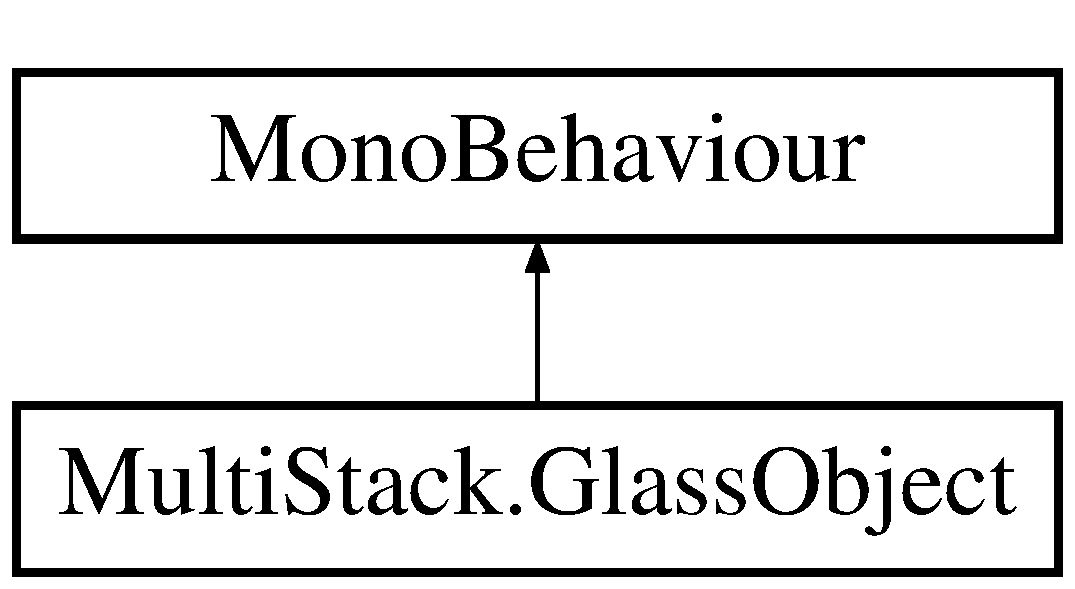
\includegraphics[height=2.000000cm]{class_multi_stack_1_1_glass_object}
\end{center}
\end{figure}
\subsection*{Public Member Functions}
\begin{DoxyCompactItemize}
\item 
void \hyperlink{class_multi_stack_1_1_glass_object_a7cc0399f29ea62b202cfaf8df9438bad}{Activate} ()
\begin{DoxyCompactList}\small\item\em Activate this instance and changes the shapes sprite to that of \hyperlink{class_multi_stack_1_1_glass_object_a9ef4bb35966c6cb6861b70ee178e5074}{Multi\+Stack.\+Glass\+Object.\+initial\+Glass\+Sprite}. \end{DoxyCompactList}\end{DoxyCompactItemize}
\subsection*{Public Attributes}
\begin{DoxyCompactItemize}
\item 
Sprite \hyperlink{class_multi_stack_1_1_glass_object_a9ef4bb35966c6cb6861b70ee178e5074}{initial\+Glass\+Sprite}
\begin{DoxyCompactList}\small\item\em The shapes sprite is changed to this sprite when it is activated. \end{DoxyCompactList}\item 
Sprite\mbox{[}$\,$\mbox{]} \hyperlink{class_multi_stack_1_1_glass_object_a3f4a1945cc951946fa2cb0c7273f63b1}{broken\+Stages}
\begin{DoxyCompactList}\small\item\em The broken stages. A glass shape can go through a number of stages before breaking. This holds the sprite for each stage. \end{DoxyCompactList}\item 
Game\+Object\mbox{[}$\,$\mbox{]} \hyperlink{class_multi_stack_1_1_glass_object_af62687ae4ee9848946633a1fb5e0a4ff}{smashed\+Object\+Prefabs}
\begin{DoxyCompactList}\small\item\em The smashed object prefabs. Spawned when the glass object breaks. \end{DoxyCompactList}\item 
Audio\+Clip \hyperlink{class_multi_stack_1_1_glass_object_a371c5cf69b11f23d2da81a3e819d6bf8}{cracked\+Audio\+Clip}
\begin{DoxyCompactList}\small\item\em The audioclip to play when the glass shape cracks. \end{DoxyCompactList}\item 
Audio\+Clip \hyperlink{class_multi_stack_1_1_glass_object_a0ffbf8da1d39767934eb87e8a2ee6710}{smashed\+Audio\+Clip}
\begin{DoxyCompactList}\small\item\em The audio clip to play when the glass shape breaks. \end{DoxyCompactList}\item 
float \hyperlink{class_multi_stack_1_1_glass_object_ae9c87a466956cd98113e0b17ad11bcd5}{required\+Force\+To\+Crack} = 2f
\begin{DoxyCompactList}\small\item\em The required force to crack. When an object collides with this shape, if the collision force is above this force then the shape cracks/breaks. \end{DoxyCompactList}\item 
float \hyperlink{class_multi_stack_1_1_glass_object_ac93340a7501f7e1db6dcffef8dea24ea}{required\+Mass\+To\+Crack} = 2f
\begin{DoxyCompactList}\small\item\em The required combined mass of shapes placed on top of this shape to cause the shape to break/crack. \end{DoxyCompactList}\item 
Layer\+Mask \hyperlink{class_multi_stack_1_1_glass_object_abce95b7ebe64b863239f56468071187b}{box\+Mask}
\begin{DoxyCompactList}\small\item\em The layermask for physics objects. \end{DoxyCompactList}\end{DoxyCompactItemize}
\subsection*{Properties}
\begin{DoxyCompactItemize}
\item 
bool \hyperlink{class_multi_stack_1_1_glass_object_a4ab5c37980ecdeea3986f7075c7ea6aa}{ready\+To\+Be\+Activated}\hspace{0.3cm}{\ttfamily  \mbox{[}get\mbox{]}}
\begin{DoxyCompactList}\small\item\em Gets a value indicating whether this \hyperlink{class_multi_stack_1_1_glass_object}{Multi\+Stack.\+Glass\+Object} is ready to be activated. \end{DoxyCompactList}\end{DoxyCompactItemize}


\subsection{Detailed Description}
Attached to any shape that can be turned into a glass shape. Handles changing a shapes sprite and breaking. 



\subsection{Member Function Documentation}
\hypertarget{class_multi_stack_1_1_glass_object_a7cc0399f29ea62b202cfaf8df9438bad}{}\index{Multi\+Stack\+::\+Glass\+Object@{Multi\+Stack\+::\+Glass\+Object}!Activate@{Activate}}
\index{Activate@{Activate}!Multi\+Stack\+::\+Glass\+Object@{Multi\+Stack\+::\+Glass\+Object}}
\subsubsection[{Activate()}]{\setlength{\rightskip}{0pt plus 5cm}void Multi\+Stack.\+Glass\+Object.\+Activate (
\begin{DoxyParamCaption}
{}
\end{DoxyParamCaption}
)}\label{class_multi_stack_1_1_glass_object_a7cc0399f29ea62b202cfaf8df9438bad}


Activate this instance and changes the shapes sprite to that of \hyperlink{class_multi_stack_1_1_glass_object_a9ef4bb35966c6cb6861b70ee178e5074}{Multi\+Stack.\+Glass\+Object.\+initial\+Glass\+Sprite}. 



\subsection{Member Data Documentation}
\hypertarget{class_multi_stack_1_1_glass_object_abce95b7ebe64b863239f56468071187b}{}\index{Multi\+Stack\+::\+Glass\+Object@{Multi\+Stack\+::\+Glass\+Object}!box\+Mask@{box\+Mask}}
\index{box\+Mask@{box\+Mask}!Multi\+Stack\+::\+Glass\+Object@{Multi\+Stack\+::\+Glass\+Object}}
\subsubsection[{box\+Mask}]{\setlength{\rightskip}{0pt plus 5cm}Layer\+Mask Multi\+Stack.\+Glass\+Object.\+box\+Mask}\label{class_multi_stack_1_1_glass_object_abce95b7ebe64b863239f56468071187b}


The layermask for physics objects. 

\hypertarget{class_multi_stack_1_1_glass_object_a3f4a1945cc951946fa2cb0c7273f63b1}{}\index{Multi\+Stack\+::\+Glass\+Object@{Multi\+Stack\+::\+Glass\+Object}!broken\+Stages@{broken\+Stages}}
\index{broken\+Stages@{broken\+Stages}!Multi\+Stack\+::\+Glass\+Object@{Multi\+Stack\+::\+Glass\+Object}}
\subsubsection[{broken\+Stages}]{\setlength{\rightskip}{0pt plus 5cm}Sprite \mbox{[}$\,$\mbox{]} Multi\+Stack.\+Glass\+Object.\+broken\+Stages}\label{class_multi_stack_1_1_glass_object_a3f4a1945cc951946fa2cb0c7273f63b1}


The broken stages. A glass shape can go through a number of stages before breaking. This holds the sprite for each stage. 

\hypertarget{class_multi_stack_1_1_glass_object_a371c5cf69b11f23d2da81a3e819d6bf8}{}\index{Multi\+Stack\+::\+Glass\+Object@{Multi\+Stack\+::\+Glass\+Object}!cracked\+Audio\+Clip@{cracked\+Audio\+Clip}}
\index{cracked\+Audio\+Clip@{cracked\+Audio\+Clip}!Multi\+Stack\+::\+Glass\+Object@{Multi\+Stack\+::\+Glass\+Object}}
\subsubsection[{cracked\+Audio\+Clip}]{\setlength{\rightskip}{0pt plus 5cm}Audio\+Clip Multi\+Stack.\+Glass\+Object.\+cracked\+Audio\+Clip}\label{class_multi_stack_1_1_glass_object_a371c5cf69b11f23d2da81a3e819d6bf8}


The audioclip to play when the glass shape cracks. 

\hypertarget{class_multi_stack_1_1_glass_object_a9ef4bb35966c6cb6861b70ee178e5074}{}\index{Multi\+Stack\+::\+Glass\+Object@{Multi\+Stack\+::\+Glass\+Object}!initial\+Glass\+Sprite@{initial\+Glass\+Sprite}}
\index{initial\+Glass\+Sprite@{initial\+Glass\+Sprite}!Multi\+Stack\+::\+Glass\+Object@{Multi\+Stack\+::\+Glass\+Object}}
\subsubsection[{initial\+Glass\+Sprite}]{\setlength{\rightskip}{0pt plus 5cm}Sprite Multi\+Stack.\+Glass\+Object.\+initial\+Glass\+Sprite}\label{class_multi_stack_1_1_glass_object_a9ef4bb35966c6cb6861b70ee178e5074}


The shapes sprite is changed to this sprite when it is activated. 

\hypertarget{class_multi_stack_1_1_glass_object_ae9c87a466956cd98113e0b17ad11bcd5}{}\index{Multi\+Stack\+::\+Glass\+Object@{Multi\+Stack\+::\+Glass\+Object}!required\+Force\+To\+Crack@{required\+Force\+To\+Crack}}
\index{required\+Force\+To\+Crack@{required\+Force\+To\+Crack}!Multi\+Stack\+::\+Glass\+Object@{Multi\+Stack\+::\+Glass\+Object}}
\subsubsection[{required\+Force\+To\+Crack}]{\setlength{\rightskip}{0pt plus 5cm}float Multi\+Stack.\+Glass\+Object.\+required\+Force\+To\+Crack = 2f}\label{class_multi_stack_1_1_glass_object_ae9c87a466956cd98113e0b17ad11bcd5}


The required force to crack. When an object collides with this shape, if the collision force is above this force then the shape cracks/breaks. 

\hypertarget{class_multi_stack_1_1_glass_object_ac93340a7501f7e1db6dcffef8dea24ea}{}\index{Multi\+Stack\+::\+Glass\+Object@{Multi\+Stack\+::\+Glass\+Object}!required\+Mass\+To\+Crack@{required\+Mass\+To\+Crack}}
\index{required\+Mass\+To\+Crack@{required\+Mass\+To\+Crack}!Multi\+Stack\+::\+Glass\+Object@{Multi\+Stack\+::\+Glass\+Object}}
\subsubsection[{required\+Mass\+To\+Crack}]{\setlength{\rightskip}{0pt plus 5cm}float Multi\+Stack.\+Glass\+Object.\+required\+Mass\+To\+Crack = 2f}\label{class_multi_stack_1_1_glass_object_ac93340a7501f7e1db6dcffef8dea24ea}


The required combined mass of shapes placed on top of this shape to cause the shape to break/crack. 

\hypertarget{class_multi_stack_1_1_glass_object_a0ffbf8da1d39767934eb87e8a2ee6710}{}\index{Multi\+Stack\+::\+Glass\+Object@{Multi\+Stack\+::\+Glass\+Object}!smashed\+Audio\+Clip@{smashed\+Audio\+Clip}}
\index{smashed\+Audio\+Clip@{smashed\+Audio\+Clip}!Multi\+Stack\+::\+Glass\+Object@{Multi\+Stack\+::\+Glass\+Object}}
\subsubsection[{smashed\+Audio\+Clip}]{\setlength{\rightskip}{0pt plus 5cm}Audio\+Clip Multi\+Stack.\+Glass\+Object.\+smashed\+Audio\+Clip}\label{class_multi_stack_1_1_glass_object_a0ffbf8da1d39767934eb87e8a2ee6710}


The audio clip to play when the glass shape breaks. 

\hypertarget{class_multi_stack_1_1_glass_object_af62687ae4ee9848946633a1fb5e0a4ff}{}\index{Multi\+Stack\+::\+Glass\+Object@{Multi\+Stack\+::\+Glass\+Object}!smashed\+Object\+Prefabs@{smashed\+Object\+Prefabs}}
\index{smashed\+Object\+Prefabs@{smashed\+Object\+Prefabs}!Multi\+Stack\+::\+Glass\+Object@{Multi\+Stack\+::\+Glass\+Object}}
\subsubsection[{smashed\+Object\+Prefabs}]{\setlength{\rightskip}{0pt plus 5cm}Game\+Object \mbox{[}$\,$\mbox{]} Multi\+Stack.\+Glass\+Object.\+smashed\+Object\+Prefabs}\label{class_multi_stack_1_1_glass_object_af62687ae4ee9848946633a1fb5e0a4ff}


The smashed object prefabs. Spawned when the glass object breaks. 



\subsection{Property Documentation}
\hypertarget{class_multi_stack_1_1_glass_object_a4ab5c37980ecdeea3986f7075c7ea6aa}{}\index{Multi\+Stack\+::\+Glass\+Object@{Multi\+Stack\+::\+Glass\+Object}!ready\+To\+Be\+Activated@{ready\+To\+Be\+Activated}}
\index{ready\+To\+Be\+Activated@{ready\+To\+Be\+Activated}!Multi\+Stack\+::\+Glass\+Object@{Multi\+Stack\+::\+Glass\+Object}}
\subsubsection[{ready\+To\+Be\+Activated}]{\setlength{\rightskip}{0pt plus 5cm}bool Multi\+Stack.\+Glass\+Object.\+ready\+To\+Be\+Activated\hspace{0.3cm}{\ttfamily [get]}}\label{class_multi_stack_1_1_glass_object_a4ab5c37980ecdeea3986f7075c7ea6aa}


Gets a value indicating whether this \hyperlink{class_multi_stack_1_1_glass_object}{Multi\+Stack.\+Glass\+Object} is ready to be activated. 

{\ttfamily true} if ready to be activated; otherwise, {\ttfamily false}.

The documentation for this class was generated from the following file\+:\begin{DoxyCompactItemize}
\item 
Multiplayer\+Stacker/\+Scripts/\+Objects/Glass\+Object.\+cs\end{DoxyCompactItemize}

\hypertarget{class_multi_stack_1_1_glass_shape_modifier}{}\section{Multi\+Stack.\+Glass\+Shape\+Modifier Class Reference}
\label{class_multi_stack_1_1_glass_shape_modifier}\index{Multi\+Stack.\+Glass\+Shape\+Modifier@{Multi\+Stack.\+Glass\+Shape\+Modifier}}


When enabled and conditions met a random shape is turned into an glass shape. Invokes \hyperlink{class_multi_stack_1_1_turn_manager_a5ecde21a2b9c4d25fa781e717a946700}{Multi\+Stack.\+Turn\+Manager.\+Change\+Shape\+To\+Glass}.  


Inheritance diagram for Multi\+Stack.\+Glass\+Shape\+Modifier\+:\begin{figure}[H]
\begin{center}
\leavevmode
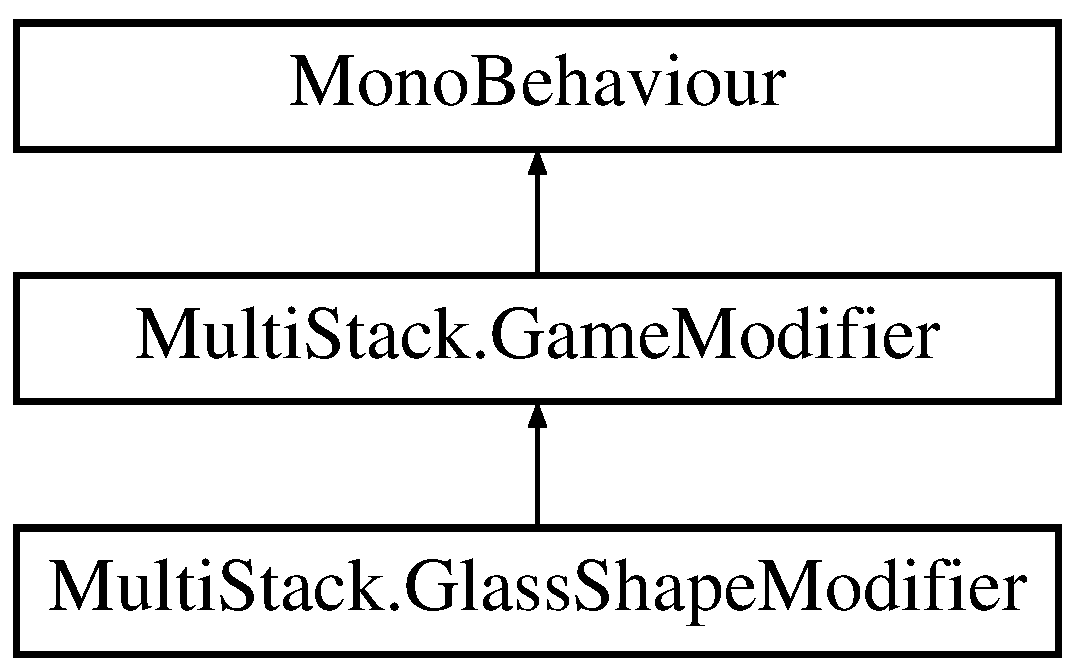
\includegraphics[height=3.000000cm]{class_multi_stack_1_1_glass_shape_modifier}
\end{center}
\end{figure}
\subsection*{Public Member Functions}
\begin{DoxyCompactItemize}
\item 
override void \hyperlink{class_multi_stack_1_1_glass_shape_modifier_aeb771b0599250515a886e0175aee746e}{Activate} ()
\begin{DoxyCompactList}\small\item\em Activate this modifier. Called at the beginning of the round. \end{DoxyCompactList}\item 
override void \hyperlink{class_multi_stack_1_1_glass_shape_modifier_a44026d971a40d8e5ce02f2611be19b0f}{Deactivate} ()
\begin{DoxyCompactList}\small\item\em Deactivate this modifier. Called before a new modifier is enabled. \end{DoxyCompactList}\item 
override bool \hyperlink{class_multi_stack_1_1_glass_shape_modifier_a75991df9c063e2fc4fd1183001df7206}{Conditions\+Met} ()
\begin{DoxyCompactList}\small\item\em Returns true if any spawned shape can be turned into an glass shape. \end{DoxyCompactList}\end{DoxyCompactItemize}
\subsection*{Additional Inherited Members}


\subsection{Detailed Description}
When enabled and conditions met a random shape is turned into an glass shape. Invokes \hyperlink{class_multi_stack_1_1_turn_manager_a5ecde21a2b9c4d25fa781e717a946700}{Multi\+Stack.\+Turn\+Manager.\+Change\+Shape\+To\+Glass}. 



\subsection{Member Function Documentation}
\hypertarget{class_multi_stack_1_1_glass_shape_modifier_aeb771b0599250515a886e0175aee746e}{}\index{Multi\+Stack\+::\+Glass\+Shape\+Modifier@{Multi\+Stack\+::\+Glass\+Shape\+Modifier}!Activate@{Activate}}
\index{Activate@{Activate}!Multi\+Stack\+::\+Glass\+Shape\+Modifier@{Multi\+Stack\+::\+Glass\+Shape\+Modifier}}
\subsubsection[{Activate()}]{\setlength{\rightskip}{0pt plus 5cm}override void Multi\+Stack.\+Glass\+Shape\+Modifier.\+Activate (
\begin{DoxyParamCaption}
{}
\end{DoxyParamCaption}
)\hspace{0.3cm}{\ttfamily [virtual]}}\label{class_multi_stack_1_1_glass_shape_modifier_aeb771b0599250515a886e0175aee746e}


Activate this modifier. Called at the beginning of the round. 



Implements \hyperlink{class_multi_stack_1_1_game_modifier_a3fb880f9728f8680bf473ac5c7f6832e}{Multi\+Stack.\+Game\+Modifier}.

\hypertarget{class_multi_stack_1_1_glass_shape_modifier_a75991df9c063e2fc4fd1183001df7206}{}\index{Multi\+Stack\+::\+Glass\+Shape\+Modifier@{Multi\+Stack\+::\+Glass\+Shape\+Modifier}!Conditions\+Met@{Conditions\+Met}}
\index{Conditions\+Met@{Conditions\+Met}!Multi\+Stack\+::\+Glass\+Shape\+Modifier@{Multi\+Stack\+::\+Glass\+Shape\+Modifier}}
\subsubsection[{Conditions\+Met()}]{\setlength{\rightskip}{0pt plus 5cm}override bool Multi\+Stack.\+Glass\+Shape\+Modifier.\+Conditions\+Met (
\begin{DoxyParamCaption}
{}
\end{DoxyParamCaption}
)\hspace{0.3cm}{\ttfamily [virtual]}}\label{class_multi_stack_1_1_glass_shape_modifier_a75991df9c063e2fc4fd1183001df7206}


Returns true if any spawned shape can be turned into an glass shape. 

\begin{DoxyReturn}{Returns}
true if a shape can be turned into glass shape.
\end{DoxyReturn}
{\ttfamily false} 

Reimplemented from \hyperlink{class_multi_stack_1_1_game_modifier_acbf45f289c8da7d9aaf129573b2c807c}{Multi\+Stack.\+Game\+Modifier}.

\hypertarget{class_multi_stack_1_1_glass_shape_modifier_a44026d971a40d8e5ce02f2611be19b0f}{}\index{Multi\+Stack\+::\+Glass\+Shape\+Modifier@{Multi\+Stack\+::\+Glass\+Shape\+Modifier}!Deactivate@{Deactivate}}
\index{Deactivate@{Deactivate}!Multi\+Stack\+::\+Glass\+Shape\+Modifier@{Multi\+Stack\+::\+Glass\+Shape\+Modifier}}
\subsubsection[{Deactivate()}]{\setlength{\rightskip}{0pt plus 5cm}override void Multi\+Stack.\+Glass\+Shape\+Modifier.\+Deactivate (
\begin{DoxyParamCaption}
{}
\end{DoxyParamCaption}
)\hspace{0.3cm}{\ttfamily [virtual]}}\label{class_multi_stack_1_1_glass_shape_modifier_a44026d971a40d8e5ce02f2611be19b0f}


Deactivate this modifier. Called before a new modifier is enabled. 



Implements \hyperlink{class_multi_stack_1_1_game_modifier_abe04db6ab31f5e5063739d8e5a3f7ad1}{Multi\+Stack.\+Game\+Modifier}.



The documentation for this class was generated from the following file\+:\begin{DoxyCompactItemize}
\item 
Multiplayer\+Stacker/\+Scripts/\+Modifiers/Glass\+Shape\+Modifier.\+cs\end{DoxyCompactItemize}

\hypertarget{class_multi_stack_1_1_gravity_modifier}{}\section{Multi\+Stack.\+Gravity\+Modifier Class Reference}
\label{class_multi_stack_1_1_gravity_modifier}\index{Multi\+Stack.\+Gravity\+Modifier@{Multi\+Stack.\+Gravity\+Modifier}}


When enabled a gravity modifier is appled to all spawned shapes.  


Inheritance diagram for Multi\+Stack.\+Gravity\+Modifier\+:\begin{figure}[H]
\begin{center}
\leavevmode
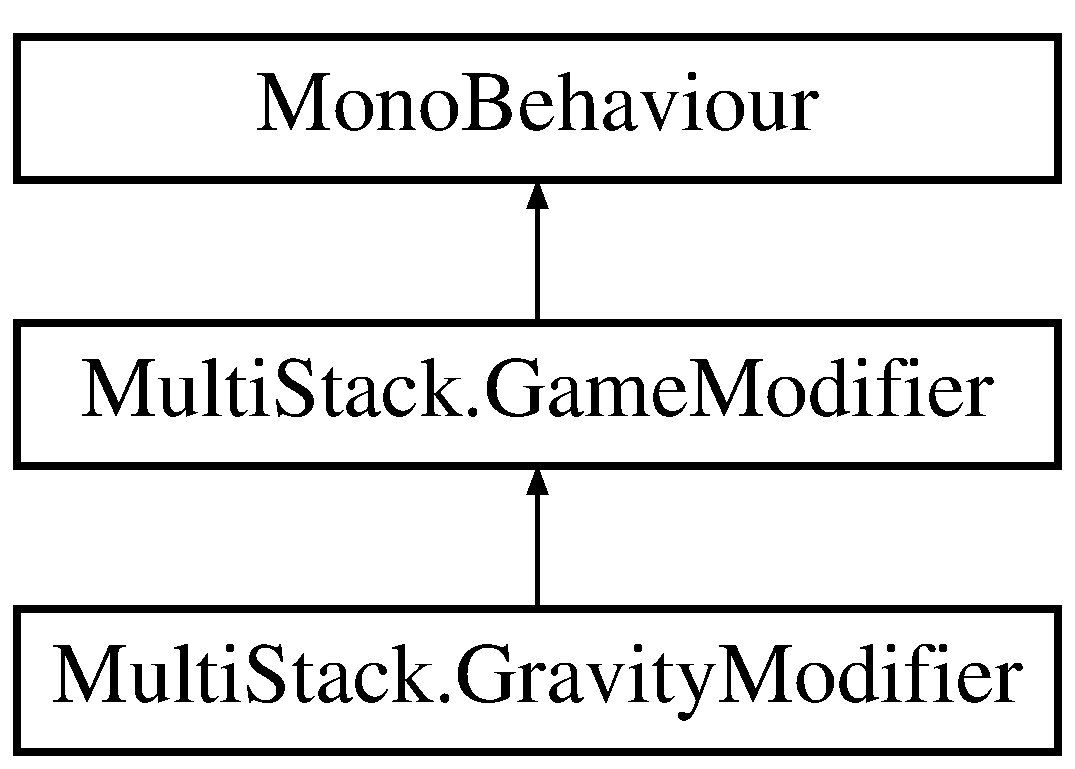
\includegraphics[height=3.000000cm]{class_multi_stack_1_1_gravity_modifier}
\end{center}
\end{figure}
\subsection*{Public Member Functions}
\begin{DoxyCompactItemize}
\item 
override void \hyperlink{class_multi_stack_1_1_gravity_modifier_a752251d8ba8759184857968d2be3327b}{Activate} ()
\begin{DoxyCompactList}\small\item\em Activate this modifier. Called at the beginning of the round. \end{DoxyCompactList}\item 
override void \hyperlink{class_multi_stack_1_1_gravity_modifier_a709194d36407f2910ceff941785d8720}{Deactivate} ()
\begin{DoxyCompactList}\small\item\em Deactivate this modifier. Called before a new modifier is enabled. \end{DoxyCompactList}\end{DoxyCompactItemize}
\subsection*{Public Attributes}
\begin{DoxyCompactItemize}
\item 
float \hyperlink{class_multi_stack_1_1_gravity_modifier_acbf32d1df1f242f10f95280c0a4b5b4d}{gravity\+Modifier}
\begin{DoxyCompactList}\small\item\em Every spawned objects gravity will be multiplied by this modifier. \end{DoxyCompactList}\item 
\hypertarget{class_multi_stack_1_1_gravity_modifier_ac6f5bf2ed7f723b9f50b4fe3b087ca48}{}\hyperlink{class_multi_stack_1_1_turn_manager}{Turn\+Manager} {\bfseries turn\+Manager}\label{class_multi_stack_1_1_gravity_modifier_ac6f5bf2ed7f723b9f50b4fe3b087ca48}

\end{DoxyCompactItemize}


\subsection{Detailed Description}
When enabled a gravity modifier is appled to all spawned shapes. 



\subsection{Member Function Documentation}
\hypertarget{class_multi_stack_1_1_gravity_modifier_a752251d8ba8759184857968d2be3327b}{}\index{Multi\+Stack\+::\+Gravity\+Modifier@{Multi\+Stack\+::\+Gravity\+Modifier}!Activate@{Activate}}
\index{Activate@{Activate}!Multi\+Stack\+::\+Gravity\+Modifier@{Multi\+Stack\+::\+Gravity\+Modifier}}
\subsubsection[{Activate()}]{\setlength{\rightskip}{0pt plus 5cm}override void Multi\+Stack.\+Gravity\+Modifier.\+Activate (
\begin{DoxyParamCaption}
{}
\end{DoxyParamCaption}
)\hspace{0.3cm}{\ttfamily [virtual]}}\label{class_multi_stack_1_1_gravity_modifier_a752251d8ba8759184857968d2be3327b}


Activate this modifier. Called at the beginning of the round. 



Implements \hyperlink{class_multi_stack_1_1_game_modifier_a3fb880f9728f8680bf473ac5c7f6832e}{Multi\+Stack.\+Game\+Modifier}.

\hypertarget{class_multi_stack_1_1_gravity_modifier_a709194d36407f2910ceff941785d8720}{}\index{Multi\+Stack\+::\+Gravity\+Modifier@{Multi\+Stack\+::\+Gravity\+Modifier}!Deactivate@{Deactivate}}
\index{Deactivate@{Deactivate}!Multi\+Stack\+::\+Gravity\+Modifier@{Multi\+Stack\+::\+Gravity\+Modifier}}
\subsubsection[{Deactivate()}]{\setlength{\rightskip}{0pt plus 5cm}override void Multi\+Stack.\+Gravity\+Modifier.\+Deactivate (
\begin{DoxyParamCaption}
{}
\end{DoxyParamCaption}
)\hspace{0.3cm}{\ttfamily [virtual]}}\label{class_multi_stack_1_1_gravity_modifier_a709194d36407f2910ceff941785d8720}


Deactivate this modifier. Called before a new modifier is enabled. 



Implements \hyperlink{class_multi_stack_1_1_game_modifier_abe04db6ab31f5e5063739d8e5a3f7ad1}{Multi\+Stack.\+Game\+Modifier}.



\subsection{Member Data Documentation}
\hypertarget{class_multi_stack_1_1_gravity_modifier_acbf32d1df1f242f10f95280c0a4b5b4d}{}\index{Multi\+Stack\+::\+Gravity\+Modifier@{Multi\+Stack\+::\+Gravity\+Modifier}!gravity\+Modifier@{gravity\+Modifier}}
\index{gravity\+Modifier@{gravity\+Modifier}!Multi\+Stack\+::\+Gravity\+Modifier@{Multi\+Stack\+::\+Gravity\+Modifier}}
\subsubsection[{gravity\+Modifier}]{\setlength{\rightskip}{0pt plus 5cm}float Multi\+Stack.\+Gravity\+Modifier.\+gravity\+Modifier}\label{class_multi_stack_1_1_gravity_modifier_acbf32d1df1f242f10f95280c0a4b5b4d}


Every spawned objects gravity will be multiplied by this modifier. 



The documentation for this class was generated from the following file\+:\begin{DoxyCompactItemize}
\item 
Multiplayer\+Stacker/\+Scripts/\+Modifiers/Gravity\+Modifier.\+cs\end{DoxyCompactItemize}

\hypertarget{class_multi_stack_1_1_height_text}{}\section{Multi\+Stack.\+Height\+Text Class Reference}
\label{class_multi_stack_1_1_height_text}\index{Multi\+Stack.\+Height\+Text@{Multi\+Stack.\+Height\+Text}}


The U\+I for the height shown during the game scene.  


Inheritance diagram for Multi\+Stack.\+Height\+Text\+:\begin{figure}[H]
\begin{center}
\leavevmode
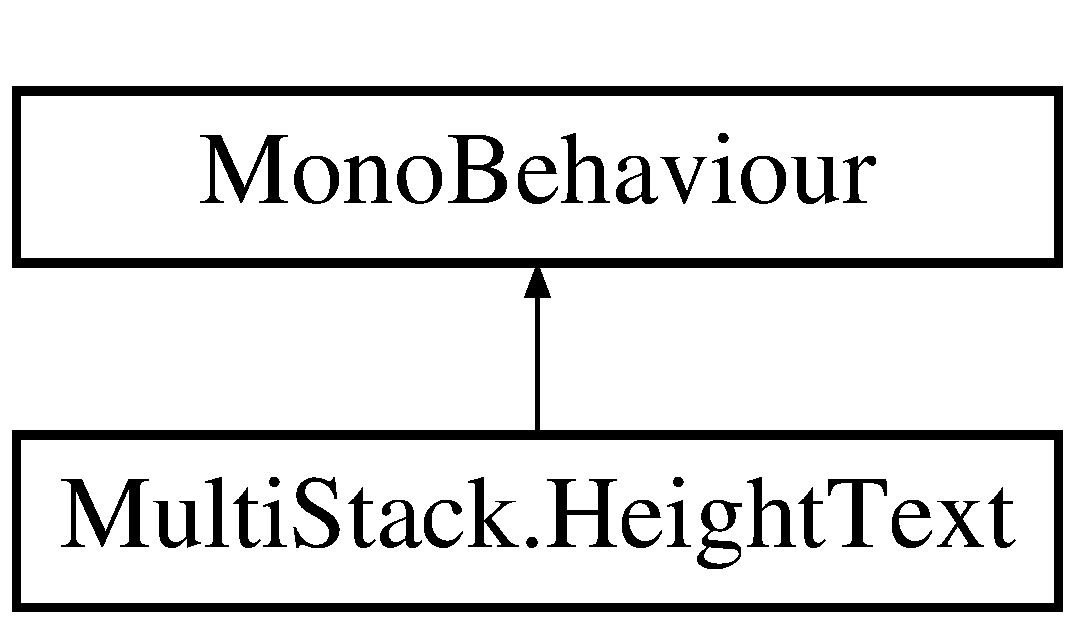
\includegraphics[height=2.000000cm]{class_multi_stack_1_1_height_text}
\end{center}
\end{figure}


\subsection{Detailed Description}
The U\+I for the height shown during the game scene. 



The documentation for this class was generated from the following file\+:\begin{DoxyCompactItemize}
\item 
Multiplayer\+Stacker/\+Scripts/\+U\+I/Height\+Text.\+cs\end{DoxyCompactItemize}

\hypertarget{class_multi_stack_1_1_highscore}{}\section{Multi\+Stack.\+Highscore Class Reference}
\label{class_multi_stack_1_1_highscore}\index{Multi\+Stack.\+Highscore@{Multi\+Stack.\+Highscore}}


The U\+I for the highest height reached on the Main menu scene.  


Inheritance diagram for Multi\+Stack.\+Highscore\+:\begin{figure}[H]
\begin{center}
\leavevmode
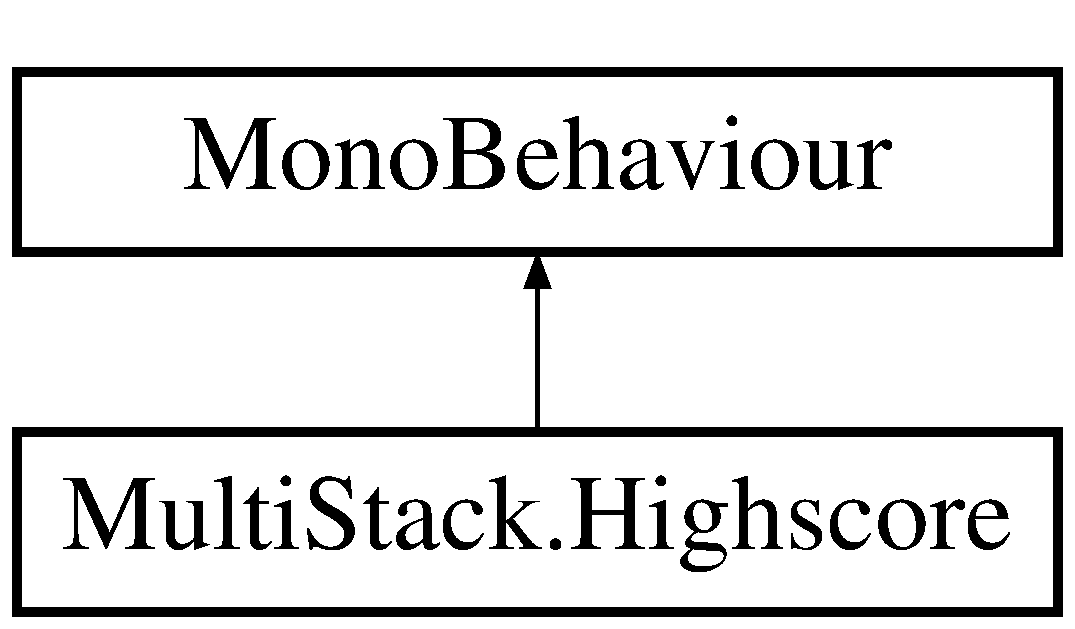
\includegraphics[height=2.000000cm]{class_multi_stack_1_1_highscore}
\end{center}
\end{figure}


\subsection{Detailed Description}
The U\+I for the highest height reached on the Main menu scene. 



The documentation for this class was generated from the following file\+:\begin{DoxyCompactItemize}
\item 
Multiplayer\+Stacker/\+Scripts/\+U\+I/Highscore.\+cs\end{DoxyCompactItemize}

\hypertarget{class_multi_stack_1_1_increase_shape_size_while_held_modifier}{}\section{Multi\+Stack.\+Increase\+Shape\+Size\+While\+Held\+Modifier Class Reference}
\label{class_multi_stack_1_1_increase_shape_size_while_held_modifier}\index{Multi\+Stack.\+Increase\+Shape\+Size\+While\+Held\+Modifier@{Multi\+Stack.\+Increase\+Shape\+Size\+While\+Held\+Modifier}}


When enabled a shapes size increases while being dragged.  


Inheritance diagram for Multi\+Stack.\+Increase\+Shape\+Size\+While\+Held\+Modifier\+:\begin{figure}[H]
\begin{center}
\leavevmode
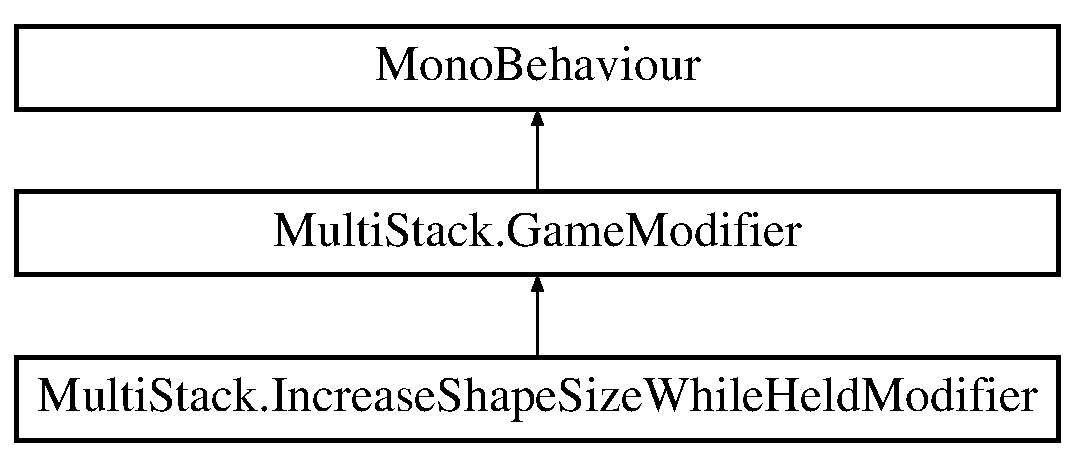
\includegraphics[height=3.000000cm]{class_multi_stack_1_1_increase_shape_size_while_held_modifier}
\end{center}
\end{figure}
\subsection*{Public Member Functions}
\begin{DoxyCompactItemize}
\item 
override void \hyperlink{class_multi_stack_1_1_increase_shape_size_while_held_modifier_a85f9b349e3654575248f7d8b4a14868e}{Activate} ()
\begin{DoxyCompactList}\small\item\em Activate this modifier. Called at the beginning of the round. \end{DoxyCompactList}\item 
override void \hyperlink{class_multi_stack_1_1_increase_shape_size_while_held_modifier_a936b7d337b1aa5febcfd6eb2ad37a016}{Deactivate} ()
\begin{DoxyCompactList}\small\item\em Deactivate this modifier. Called before a new modifier is enabled. \end{DoxyCompactList}\end{DoxyCompactItemize}
\subsection*{Public Attributes}
\begin{DoxyCompactItemize}
\item 
\hypertarget{class_multi_stack_1_1_increase_shape_size_while_held_modifier_a6c39a507036c81a6eeddf794801a8027}{}\hyperlink{class_multi_stack_1_1_click_handler}{Click\+Handler} {\bfseries click\+Handler}\label{class_multi_stack_1_1_increase_shape_size_while_held_modifier_a6c39a507036c81a6eeddf794801a8027}

\end{DoxyCompactItemize}


\subsection{Detailed Description}
When enabled a shapes size increases while being dragged. 



\subsection{Member Function Documentation}
\hypertarget{class_multi_stack_1_1_increase_shape_size_while_held_modifier_a85f9b349e3654575248f7d8b4a14868e}{}\index{Multi\+Stack\+::\+Increase\+Shape\+Size\+While\+Held\+Modifier@{Multi\+Stack\+::\+Increase\+Shape\+Size\+While\+Held\+Modifier}!Activate@{Activate}}
\index{Activate@{Activate}!Multi\+Stack\+::\+Increase\+Shape\+Size\+While\+Held\+Modifier@{Multi\+Stack\+::\+Increase\+Shape\+Size\+While\+Held\+Modifier}}
\subsubsection[{Activate()}]{\setlength{\rightskip}{0pt plus 5cm}override void Multi\+Stack.\+Increase\+Shape\+Size\+While\+Held\+Modifier.\+Activate (
\begin{DoxyParamCaption}
{}
\end{DoxyParamCaption}
)\hspace{0.3cm}{\ttfamily [virtual]}}\label{class_multi_stack_1_1_increase_shape_size_while_held_modifier_a85f9b349e3654575248f7d8b4a14868e}


Activate this modifier. Called at the beginning of the round. 



Implements \hyperlink{class_multi_stack_1_1_game_modifier_a3fb880f9728f8680bf473ac5c7f6832e}{Multi\+Stack.\+Game\+Modifier}.

\hypertarget{class_multi_stack_1_1_increase_shape_size_while_held_modifier_a936b7d337b1aa5febcfd6eb2ad37a016}{}\index{Multi\+Stack\+::\+Increase\+Shape\+Size\+While\+Held\+Modifier@{Multi\+Stack\+::\+Increase\+Shape\+Size\+While\+Held\+Modifier}!Deactivate@{Deactivate}}
\index{Deactivate@{Deactivate}!Multi\+Stack\+::\+Increase\+Shape\+Size\+While\+Held\+Modifier@{Multi\+Stack\+::\+Increase\+Shape\+Size\+While\+Held\+Modifier}}
\subsubsection[{Deactivate()}]{\setlength{\rightskip}{0pt plus 5cm}override void Multi\+Stack.\+Increase\+Shape\+Size\+While\+Held\+Modifier.\+Deactivate (
\begin{DoxyParamCaption}
{}
\end{DoxyParamCaption}
)\hspace{0.3cm}{\ttfamily [virtual]}}\label{class_multi_stack_1_1_increase_shape_size_while_held_modifier_a936b7d337b1aa5febcfd6eb2ad37a016}


Deactivate this modifier. Called before a new modifier is enabled. 



Implements \hyperlink{class_multi_stack_1_1_game_modifier_abe04db6ab31f5e5063739d8e5a3f7ad1}{Multi\+Stack.\+Game\+Modifier}.



The documentation for this class was generated from the following file\+:\begin{DoxyCompactItemize}
\item 
Multiplayer\+Stacker/\+Scripts/\+Modifiers/Increase\+Shape\+Size\+While\+Held\+Modifier.\+cs\end{DoxyCompactItemize}

\hypertarget{class_multi_stack_1_1_main_menu}{}\section{Multi\+Stack.\+Main\+Menu Class Reference}
\label{class_multi_stack_1_1_main_menu}\index{Multi\+Stack.\+Main\+Menu@{Multi\+Stack.\+Main\+Menu}}


Handles the U\+I for main menu and number of players select scene.  


Inheritance diagram for Multi\+Stack.\+Main\+Menu\+:\begin{figure}[H]
\begin{center}
\leavevmode
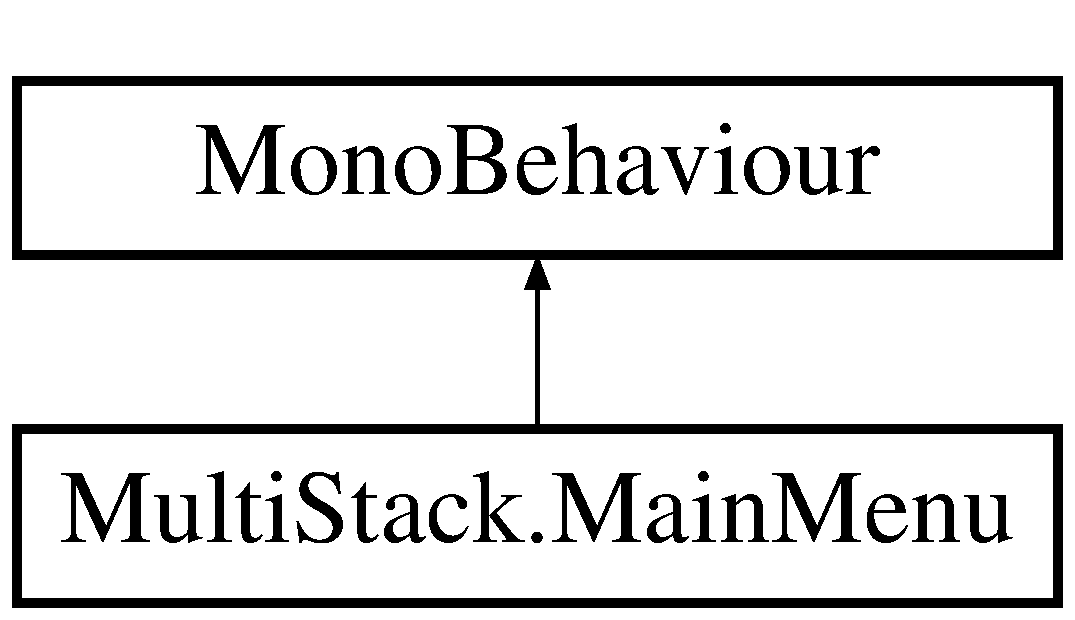
\includegraphics[height=2.000000cm]{class_multi_stack_1_1_main_menu}
\end{center}
\end{figure}
\subsection*{Public Member Functions}
\begin{DoxyCompactItemize}
\item 
void \hyperlink{class_multi_stack_1_1_main_menu_ae2fe990ea5367c5613591dbd23ecf9d8}{Player\+Box\+Placed} ()
\begin{DoxyCompactList}\small\item\em Called when the player places a box on the platform. \end{DoxyCompactList}\item 
void \hyperlink{class_multi_stack_1_1_main_menu_a1e974e00f83bacb1d410a9ea6ec73e32}{Player\+Box\+Removed} ()
\begin{DoxyCompactList}\small\item\em Called when the player removes a box from the platform. \end{DoxyCompactList}\item 
void \hyperlink{class_multi_stack_1_1_main_menu_a48eb0a0757e1a7b85cb34e334da484fa}{Play\+Button\+Pressed} ()
\begin{DoxyCompactList}\small\item\em Called when the play button has been pressed. If it is the first time it has been pressed, then it pans the camera down and then spawns the boxes else it loads the game scene. \end{DoxyCompactList}\end{DoxyCompactItemize}
\subsection*{Public Attributes}
\begin{DoxyCompactItemize}
\item 
\hyperlink{class_multi_stack_1_1_game_text}{Game\+Text} \hyperlink{class_multi_stack_1_1_main_menu_a6fd09504dbf98f1464f65e15d897e8e4}{title\+Text}
\begin{DoxyCompactList}\small\item\em The title text. \end{DoxyCompactList}\item 
\hyperlink{class_multi_stack_1_1_game_text}{Game\+Text} \hyperlink{class_multi_stack_1_1_main_menu_a67a98e0ca8c571f820e68e586ba53072}{num\+Of\+Players\+Text}
\begin{DoxyCompactList}\small\item\em The number of players text. \end{DoxyCompactList}\item 
\hyperlink{class_multi_stack_1_1_game_text}{Game\+Text} \hyperlink{class_multi_stack_1_1_main_menu_ae6d2e9ea930343eeadd0d2405149d347}{other\+Text}
\begin{DoxyCompactList}\small\item\em The other text. This is used to show messages to the player. \end{DoxyCompactList}\item 
Rect\+Transform \hyperlink{class_multi_stack_1_1_main_menu_ad0770c7731b1bc84fe9214e576f84b1c}{play\+Button}
\begin{DoxyCompactList}\small\item\em The play button rect transform. Used to translate the button when moving to the number of players screen. \end{DoxyCompactList}\item 
Game\+Object \hyperlink{class_multi_stack_1_1_main_menu_a423b9ab552b7a5e2068b33e8276931ea}{player\+Box\+Prefab}
\begin{DoxyCompactList}\small\item\em The prefab for the physics boxes used in the number of players select screen. \end{DoxyCompactList}\item 
Transform\mbox{[}$\,$\mbox{]} \hyperlink{class_multi_stack_1_1_main_menu_af217845475c893bd3d6269933a269892}{player\+Box\+Spawn\+Locations}
\begin{DoxyCompactList}\small\item\em The box spawn locations. \end{DoxyCompactList}\end{DoxyCompactItemize}


\subsection{Detailed Description}
Handles the U\+I for main menu and number of players select scene. 



\subsection{Member Function Documentation}
\hypertarget{class_multi_stack_1_1_main_menu_a48eb0a0757e1a7b85cb34e334da484fa}{}\index{Multi\+Stack\+::\+Main\+Menu@{Multi\+Stack\+::\+Main\+Menu}!Play\+Button\+Pressed@{Play\+Button\+Pressed}}
\index{Play\+Button\+Pressed@{Play\+Button\+Pressed}!Multi\+Stack\+::\+Main\+Menu@{Multi\+Stack\+::\+Main\+Menu}}
\subsubsection[{Play\+Button\+Pressed()}]{\setlength{\rightskip}{0pt plus 5cm}void Multi\+Stack.\+Main\+Menu.\+Play\+Button\+Pressed (
\begin{DoxyParamCaption}
{}
\end{DoxyParamCaption}
)}\label{class_multi_stack_1_1_main_menu_a48eb0a0757e1a7b85cb34e334da484fa}


Called when the play button has been pressed. If it is the first time it has been pressed, then it pans the camera down and then spawns the boxes else it loads the game scene. 

\hypertarget{class_multi_stack_1_1_main_menu_ae2fe990ea5367c5613591dbd23ecf9d8}{}\index{Multi\+Stack\+::\+Main\+Menu@{Multi\+Stack\+::\+Main\+Menu}!Player\+Box\+Placed@{Player\+Box\+Placed}}
\index{Player\+Box\+Placed@{Player\+Box\+Placed}!Multi\+Stack\+::\+Main\+Menu@{Multi\+Stack\+::\+Main\+Menu}}
\subsubsection[{Player\+Box\+Placed()}]{\setlength{\rightskip}{0pt plus 5cm}void Multi\+Stack.\+Main\+Menu.\+Player\+Box\+Placed (
\begin{DoxyParamCaption}
{}
\end{DoxyParamCaption}
)}\label{class_multi_stack_1_1_main_menu_ae2fe990ea5367c5613591dbd23ecf9d8}


Called when the player places a box on the platform. 

\hypertarget{class_multi_stack_1_1_main_menu_a1e974e00f83bacb1d410a9ea6ec73e32}{}\index{Multi\+Stack\+::\+Main\+Menu@{Multi\+Stack\+::\+Main\+Menu}!Player\+Box\+Removed@{Player\+Box\+Removed}}
\index{Player\+Box\+Removed@{Player\+Box\+Removed}!Multi\+Stack\+::\+Main\+Menu@{Multi\+Stack\+::\+Main\+Menu}}
\subsubsection[{Player\+Box\+Removed()}]{\setlength{\rightskip}{0pt plus 5cm}void Multi\+Stack.\+Main\+Menu.\+Player\+Box\+Removed (
\begin{DoxyParamCaption}
{}
\end{DoxyParamCaption}
)}\label{class_multi_stack_1_1_main_menu_a1e974e00f83bacb1d410a9ea6ec73e32}


Called when the player removes a box from the platform. 



\subsection{Member Data Documentation}
\hypertarget{class_multi_stack_1_1_main_menu_a67a98e0ca8c571f820e68e586ba53072}{}\index{Multi\+Stack\+::\+Main\+Menu@{Multi\+Stack\+::\+Main\+Menu}!num\+Of\+Players\+Text@{num\+Of\+Players\+Text}}
\index{num\+Of\+Players\+Text@{num\+Of\+Players\+Text}!Multi\+Stack\+::\+Main\+Menu@{Multi\+Stack\+::\+Main\+Menu}}
\subsubsection[{num\+Of\+Players\+Text}]{\setlength{\rightskip}{0pt plus 5cm}{\bf Game\+Text} Multi\+Stack.\+Main\+Menu.\+num\+Of\+Players\+Text}\label{class_multi_stack_1_1_main_menu_a67a98e0ca8c571f820e68e586ba53072}


The number of players text. 

\hypertarget{class_multi_stack_1_1_main_menu_ae6d2e9ea930343eeadd0d2405149d347}{}\index{Multi\+Stack\+::\+Main\+Menu@{Multi\+Stack\+::\+Main\+Menu}!other\+Text@{other\+Text}}
\index{other\+Text@{other\+Text}!Multi\+Stack\+::\+Main\+Menu@{Multi\+Stack\+::\+Main\+Menu}}
\subsubsection[{other\+Text}]{\setlength{\rightskip}{0pt plus 5cm}{\bf Game\+Text} Multi\+Stack.\+Main\+Menu.\+other\+Text}\label{class_multi_stack_1_1_main_menu_ae6d2e9ea930343eeadd0d2405149d347}


The other text. This is used to show messages to the player. 

\hypertarget{class_multi_stack_1_1_main_menu_ad0770c7731b1bc84fe9214e576f84b1c}{}\index{Multi\+Stack\+::\+Main\+Menu@{Multi\+Stack\+::\+Main\+Menu}!play\+Button@{play\+Button}}
\index{play\+Button@{play\+Button}!Multi\+Stack\+::\+Main\+Menu@{Multi\+Stack\+::\+Main\+Menu}}
\subsubsection[{play\+Button}]{\setlength{\rightskip}{0pt plus 5cm}Rect\+Transform Multi\+Stack.\+Main\+Menu.\+play\+Button}\label{class_multi_stack_1_1_main_menu_ad0770c7731b1bc84fe9214e576f84b1c}


The play button rect transform. Used to translate the button when moving to the number of players screen. 

\hypertarget{class_multi_stack_1_1_main_menu_a423b9ab552b7a5e2068b33e8276931ea}{}\index{Multi\+Stack\+::\+Main\+Menu@{Multi\+Stack\+::\+Main\+Menu}!player\+Box\+Prefab@{player\+Box\+Prefab}}
\index{player\+Box\+Prefab@{player\+Box\+Prefab}!Multi\+Stack\+::\+Main\+Menu@{Multi\+Stack\+::\+Main\+Menu}}
\subsubsection[{player\+Box\+Prefab}]{\setlength{\rightskip}{0pt plus 5cm}Game\+Object Multi\+Stack.\+Main\+Menu.\+player\+Box\+Prefab}\label{class_multi_stack_1_1_main_menu_a423b9ab552b7a5e2068b33e8276931ea}


The prefab for the physics boxes used in the number of players select screen. 

\hypertarget{class_multi_stack_1_1_main_menu_af217845475c893bd3d6269933a269892}{}\index{Multi\+Stack\+::\+Main\+Menu@{Multi\+Stack\+::\+Main\+Menu}!player\+Box\+Spawn\+Locations@{player\+Box\+Spawn\+Locations}}
\index{player\+Box\+Spawn\+Locations@{player\+Box\+Spawn\+Locations}!Multi\+Stack\+::\+Main\+Menu@{Multi\+Stack\+::\+Main\+Menu}}
\subsubsection[{player\+Box\+Spawn\+Locations}]{\setlength{\rightskip}{0pt plus 5cm}Transform \mbox{[}$\,$\mbox{]} Multi\+Stack.\+Main\+Menu.\+player\+Box\+Spawn\+Locations}\label{class_multi_stack_1_1_main_menu_af217845475c893bd3d6269933a269892}


The box spawn locations. 

\hypertarget{class_multi_stack_1_1_main_menu_a6fd09504dbf98f1464f65e15d897e8e4}{}\index{Multi\+Stack\+::\+Main\+Menu@{Multi\+Stack\+::\+Main\+Menu}!title\+Text@{title\+Text}}
\index{title\+Text@{title\+Text}!Multi\+Stack\+::\+Main\+Menu@{Multi\+Stack\+::\+Main\+Menu}}
\subsubsection[{title\+Text}]{\setlength{\rightskip}{0pt plus 5cm}{\bf Game\+Text} Multi\+Stack.\+Main\+Menu.\+title\+Text}\label{class_multi_stack_1_1_main_menu_a6fd09504dbf98f1464f65e15d897e8e4}


The title text. 



The documentation for this class was generated from the following file\+:\begin{DoxyCompactItemize}
\item 
Multiplayer\+Stacker/\+Scripts/\+U\+I/Main\+Menu.\+cs\end{DoxyCompactItemize}

\hypertarget{class_multi_stack_1_1_move_time}{}\section{Multi\+Stack.\+Move\+Time Class Reference}
\label{class_multi_stack_1_1_move_time}\index{Multi\+Stack.\+Move\+Time@{Multi\+Stack.\+Move\+Time}}


Responsible for updating the current players move time.  


Inheritance diagram for Multi\+Stack.\+Move\+Time\+:\begin{figure}[H]
\begin{center}
\leavevmode
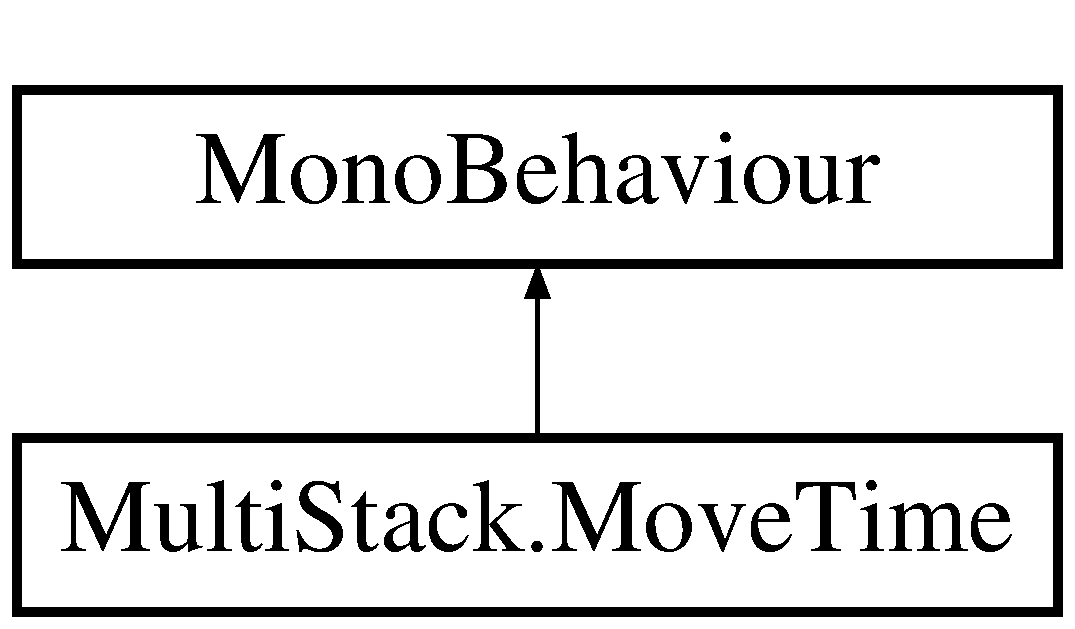
\includegraphics[height=2.000000cm]{class_multi_stack_1_1_move_time}
\end{center}
\end{figure}
\subsection*{Public Attributes}
\begin{DoxyCompactItemize}
\item 
int \hyperlink{class_multi_stack_1_1_move_time_a1f9dcd4f0bb8bd038f486c5a0ac2478e}{low\+On\+Time\+Threshold}
\begin{DoxyCompactList}\small\item\em The low on time threshold. When the players current time is below this threshold the time will pulse and move to the centre of the screen, \end{DoxyCompactList}\item 
Color \hyperlink{class_multi_stack_1_1_move_time_a31e3512da14ba52898e306c4d8b63320}{normal\+Time\+Text\+Colour}
\begin{DoxyCompactList}\small\item\em The colour of the countdown text when the time is above the \hyperlink{class_multi_stack_1_1_move_time_a1f9dcd4f0bb8bd038f486c5a0ac2478e}{Multi\+Stack.\+Move\+Time.\+low\+On\+Time\+Threshold}. \end{DoxyCompactList}\item 
Color \hyperlink{class_multi_stack_1_1_move_time_a4de86ca47dc6be9e38117ee65a1677e6}{low\+Time\+Text\+Colour}
\begin{DoxyCompactList}\small\item\em The colour of the countdown text when the time is below the \hyperlink{class_multi_stack_1_1_move_time_a1f9dcd4f0bb8bd038f486c5a0ac2478e}{Multi\+Stack.\+Move\+Time.\+low\+On\+Time\+Threshold}. \end{DoxyCompactList}\end{DoxyCompactItemize}


\subsection{Detailed Description}
Responsible for updating the current players move time. 



\subsection{Member Data Documentation}
\hypertarget{class_multi_stack_1_1_move_time_a1f9dcd4f0bb8bd038f486c5a0ac2478e}{}\index{Multi\+Stack\+::\+Move\+Time@{Multi\+Stack\+::\+Move\+Time}!low\+On\+Time\+Threshold@{low\+On\+Time\+Threshold}}
\index{low\+On\+Time\+Threshold@{low\+On\+Time\+Threshold}!Multi\+Stack\+::\+Move\+Time@{Multi\+Stack\+::\+Move\+Time}}
\subsubsection[{low\+On\+Time\+Threshold}]{\setlength{\rightskip}{0pt plus 5cm}int Multi\+Stack.\+Move\+Time.\+low\+On\+Time\+Threshold}\label{class_multi_stack_1_1_move_time_a1f9dcd4f0bb8bd038f486c5a0ac2478e}


The low on time threshold. When the players current time is below this threshold the time will pulse and move to the centre of the screen, 

\hypertarget{class_multi_stack_1_1_move_time_a4de86ca47dc6be9e38117ee65a1677e6}{}\index{Multi\+Stack\+::\+Move\+Time@{Multi\+Stack\+::\+Move\+Time}!low\+Time\+Text\+Colour@{low\+Time\+Text\+Colour}}
\index{low\+Time\+Text\+Colour@{low\+Time\+Text\+Colour}!Multi\+Stack\+::\+Move\+Time@{Multi\+Stack\+::\+Move\+Time}}
\subsubsection[{low\+Time\+Text\+Colour}]{\setlength{\rightskip}{0pt plus 5cm}Color Multi\+Stack.\+Move\+Time.\+low\+Time\+Text\+Colour}\label{class_multi_stack_1_1_move_time_a4de86ca47dc6be9e38117ee65a1677e6}


The colour of the countdown text when the time is below the \hyperlink{class_multi_stack_1_1_move_time_a1f9dcd4f0bb8bd038f486c5a0ac2478e}{Multi\+Stack.\+Move\+Time.\+low\+On\+Time\+Threshold}. 

\hypertarget{class_multi_stack_1_1_move_time_a31e3512da14ba52898e306c4d8b63320}{}\index{Multi\+Stack\+::\+Move\+Time@{Multi\+Stack\+::\+Move\+Time}!normal\+Time\+Text\+Colour@{normal\+Time\+Text\+Colour}}
\index{normal\+Time\+Text\+Colour@{normal\+Time\+Text\+Colour}!Multi\+Stack\+::\+Move\+Time@{Multi\+Stack\+::\+Move\+Time}}
\subsubsection[{normal\+Time\+Text\+Colour}]{\setlength{\rightskip}{0pt plus 5cm}Color Multi\+Stack.\+Move\+Time.\+normal\+Time\+Text\+Colour}\label{class_multi_stack_1_1_move_time_a31e3512da14ba52898e306c4d8b63320}


The colour of the countdown text when the time is above the \hyperlink{class_multi_stack_1_1_move_time_a1f9dcd4f0bb8bd038f486c5a0ac2478e}{Multi\+Stack.\+Move\+Time.\+low\+On\+Time\+Threshold}. 



The documentation for this class was generated from the following file\+:\begin{DoxyCompactItemize}
\item 
Multiplayer\+Stacker/\+Scripts/\+U\+I/Move\+Time.\+cs\end{DoxyCompactItemize}

\hypertarget{class_multi_stack_1_1_one_shape_modifier}{}\section{Multi\+Stack.\+One\+Shape\+Modifier Class Reference}
\label{class_multi_stack_1_1_one_shape_modifier}\index{Multi\+Stack.\+One\+Shape\+Modifier@{Multi\+Stack.\+One\+Shape\+Modifier}}


When enabled only one shape specified by \hyperlink{class_multi_stack_1_1_one_shape_modifier_a5724e9f0dc3edb5f97363252a67b5db5}{Multi\+Stack.\+One\+Shape\+Modifier.\+shape} will be spawned for that round.  


Inheritance diagram for Multi\+Stack.\+One\+Shape\+Modifier\+:\begin{figure}[H]
\begin{center}
\leavevmode
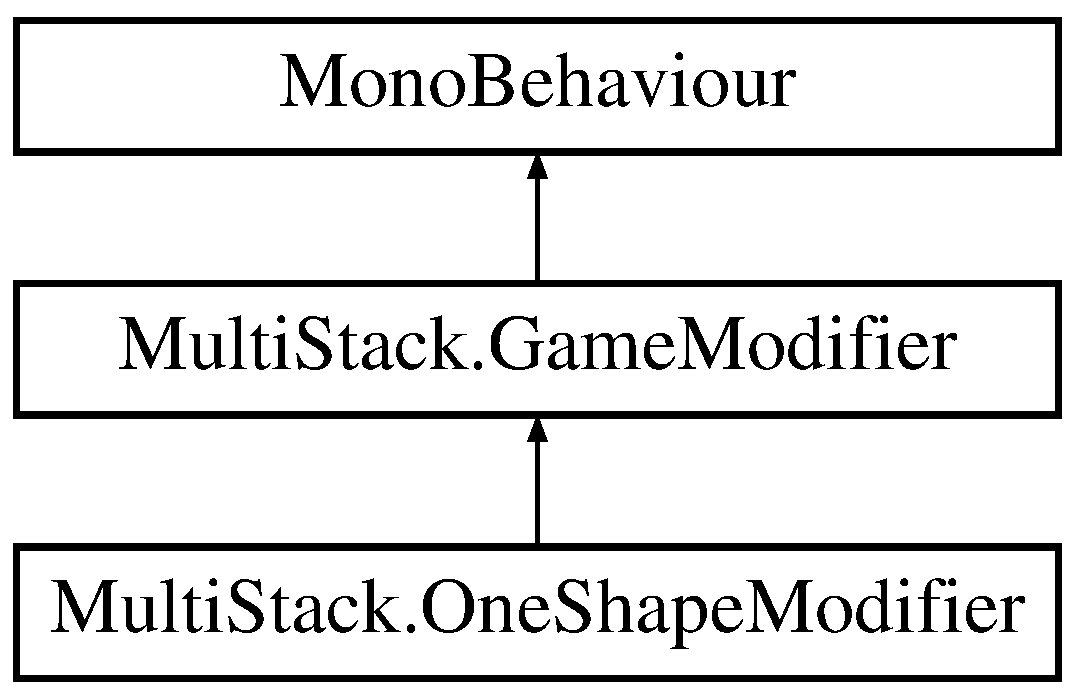
\includegraphics[height=3.000000cm]{class_multi_stack_1_1_one_shape_modifier}
\end{center}
\end{figure}
\subsection*{Public Member Functions}
\begin{DoxyCompactItemize}
\item 
override void \hyperlink{class_multi_stack_1_1_one_shape_modifier_a36e475d44744e4f6d5b3dbe1b1ee3a16}{Activate} ()
\begin{DoxyCompactList}\small\item\em Activate this modifier. Called at the beginning of the round. \end{DoxyCompactList}\item 
override void \hyperlink{class_multi_stack_1_1_one_shape_modifier_a26f5a41e291d04df9a55fd931ff834ec}{Deactivate} ()
\begin{DoxyCompactList}\small\item\em Deactivate this modifier. Called before a new modifier is enabled. \end{DoxyCompactList}\end{DoxyCompactItemize}
\subsection*{Public Attributes}
\begin{DoxyCompactItemize}
\item 
\hyperlink{namespace_multi_stack_ac7f637887fea673ceeae6fdd0598c048}{Shape} \hyperlink{class_multi_stack_1_1_one_shape_modifier_a5724e9f0dc3edb5f97363252a67b5db5}{shape}
\begin{DoxyCompactList}\small\item\em The sole shape to be spawned this round. \end{DoxyCompactList}\end{DoxyCompactItemize}


\subsection{Detailed Description}
When enabled only one shape specified by \hyperlink{class_multi_stack_1_1_one_shape_modifier_a5724e9f0dc3edb5f97363252a67b5db5}{Multi\+Stack.\+One\+Shape\+Modifier.\+shape} will be spawned for that round. 



\subsection{Member Function Documentation}
\hypertarget{class_multi_stack_1_1_one_shape_modifier_a36e475d44744e4f6d5b3dbe1b1ee3a16}{}\index{Multi\+Stack\+::\+One\+Shape\+Modifier@{Multi\+Stack\+::\+One\+Shape\+Modifier}!Activate@{Activate}}
\index{Activate@{Activate}!Multi\+Stack\+::\+One\+Shape\+Modifier@{Multi\+Stack\+::\+One\+Shape\+Modifier}}
\subsubsection[{Activate()}]{\setlength{\rightskip}{0pt plus 5cm}override void Multi\+Stack.\+One\+Shape\+Modifier.\+Activate (
\begin{DoxyParamCaption}
{}
\end{DoxyParamCaption}
)\hspace{0.3cm}{\ttfamily [virtual]}}\label{class_multi_stack_1_1_one_shape_modifier_a36e475d44744e4f6d5b3dbe1b1ee3a16}


Activate this modifier. Called at the beginning of the round. 



Implements \hyperlink{class_multi_stack_1_1_game_modifier_a3fb880f9728f8680bf473ac5c7f6832e}{Multi\+Stack.\+Game\+Modifier}.

\hypertarget{class_multi_stack_1_1_one_shape_modifier_a26f5a41e291d04df9a55fd931ff834ec}{}\index{Multi\+Stack\+::\+One\+Shape\+Modifier@{Multi\+Stack\+::\+One\+Shape\+Modifier}!Deactivate@{Deactivate}}
\index{Deactivate@{Deactivate}!Multi\+Stack\+::\+One\+Shape\+Modifier@{Multi\+Stack\+::\+One\+Shape\+Modifier}}
\subsubsection[{Deactivate()}]{\setlength{\rightskip}{0pt plus 5cm}override void Multi\+Stack.\+One\+Shape\+Modifier.\+Deactivate (
\begin{DoxyParamCaption}
{}
\end{DoxyParamCaption}
)\hspace{0.3cm}{\ttfamily [virtual]}}\label{class_multi_stack_1_1_one_shape_modifier_a26f5a41e291d04df9a55fd931ff834ec}


Deactivate this modifier. Called before a new modifier is enabled. 



Implements \hyperlink{class_multi_stack_1_1_game_modifier_abe04db6ab31f5e5063739d8e5a3f7ad1}{Multi\+Stack.\+Game\+Modifier}.



\subsection{Member Data Documentation}
\hypertarget{class_multi_stack_1_1_one_shape_modifier_a5724e9f0dc3edb5f97363252a67b5db5}{}\index{Multi\+Stack\+::\+One\+Shape\+Modifier@{Multi\+Stack\+::\+One\+Shape\+Modifier}!shape@{shape}}
\index{shape@{shape}!Multi\+Stack\+::\+One\+Shape\+Modifier@{Multi\+Stack\+::\+One\+Shape\+Modifier}}
\subsubsection[{shape}]{\setlength{\rightskip}{0pt plus 5cm}{\bf Shape} Multi\+Stack.\+One\+Shape\+Modifier.\+shape}\label{class_multi_stack_1_1_one_shape_modifier_a5724e9f0dc3edb5f97363252a67b5db5}


The sole shape to be spawned this round. 



The documentation for this class was generated from the following file\+:\begin{DoxyCompactItemize}
\item 
Multiplayer\+Stacker/\+Scripts/\+Modifiers/One\+Shape\+Modifier.\+cs\end{DoxyCompactItemize}

\hypertarget{class_multi_stack_1_1_player_box_placed}{}\section{Multi\+Stack.\+Player\+Box\+Placed Class Reference}
\label{class_multi_stack_1_1_player_box_placed}\index{Multi\+Stack.\+Player\+Box\+Placed@{Multi\+Stack.\+Player\+Box\+Placed}}


Used during the number of player selection scene. Handles alerting \hyperlink{class_multi_stack_1_1_main_menu}{Multi\+Stack.\+Main\+Menu} when a box is placed by invoking \hyperlink{class_multi_stack_1_1_main_menu_ae2fe990ea5367c5613591dbd23ecf9d8}{Multi\+Stack.\+Main\+Menu.\+Player\+Box\+Placed} and \hyperlink{class_multi_stack_1_1_main_menu_a1e974e00f83bacb1d410a9ea6ec73e32}{Multi\+Stack.\+Main\+Menu.\+Player\+Box\+Removed}.  


Inheritance diagram for Multi\+Stack.\+Player\+Box\+Placed\+:\begin{figure}[H]
\begin{center}
\leavevmode
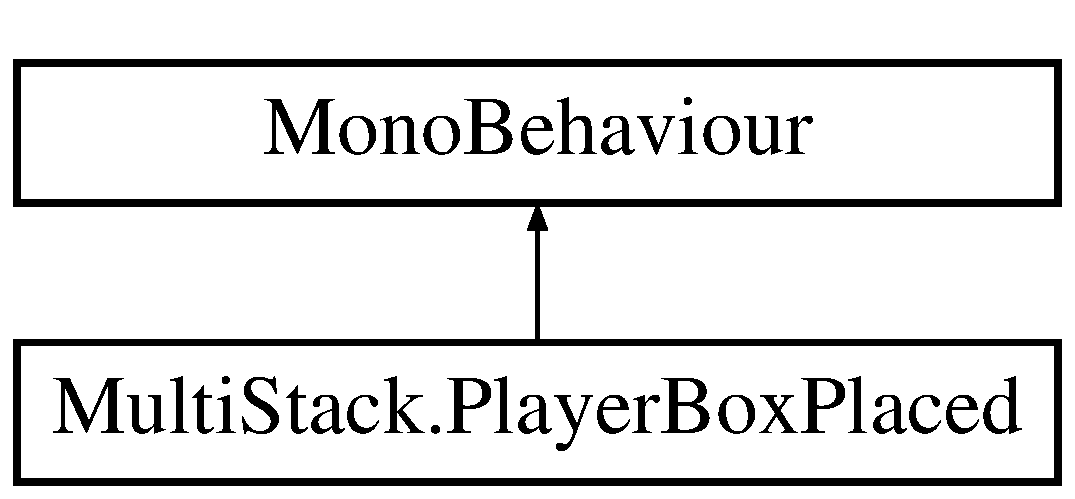
\includegraphics[height=2.000000cm]{class_multi_stack_1_1_player_box_placed}
\end{center}
\end{figure}


\subsection{Detailed Description}
Used during the number of player selection scene. Handles alerting \hyperlink{class_multi_stack_1_1_main_menu}{Multi\+Stack.\+Main\+Menu} when a box is placed by invoking \hyperlink{class_multi_stack_1_1_main_menu_ae2fe990ea5367c5613591dbd23ecf9d8}{Multi\+Stack.\+Main\+Menu.\+Player\+Box\+Placed} and \hyperlink{class_multi_stack_1_1_main_menu_a1e974e00f83bacb1d410a9ea6ec73e32}{Multi\+Stack.\+Main\+Menu.\+Player\+Box\+Removed}. 



The documentation for this class was generated from the following file\+:\begin{DoxyCompactItemize}
\item 
Multiplayer\+Stacker/\+Scripts/\+U\+I/Player\+Box\+Placed.\+cs\end{DoxyCompactItemize}

\hypertarget{class_multi_stack_1_1_player_colours}{}\section{Multi\+Stack.\+Player\+Colours Class Reference}
\label{class_multi_stack_1_1_player_colours}\index{Multi\+Stack.\+Player\+Colours@{Multi\+Stack.\+Player\+Colours}}


Holds the coours for each player.  


Inheritance diagram for Multi\+Stack.\+Player\+Colours\+:\begin{figure}[H]
\begin{center}
\leavevmode
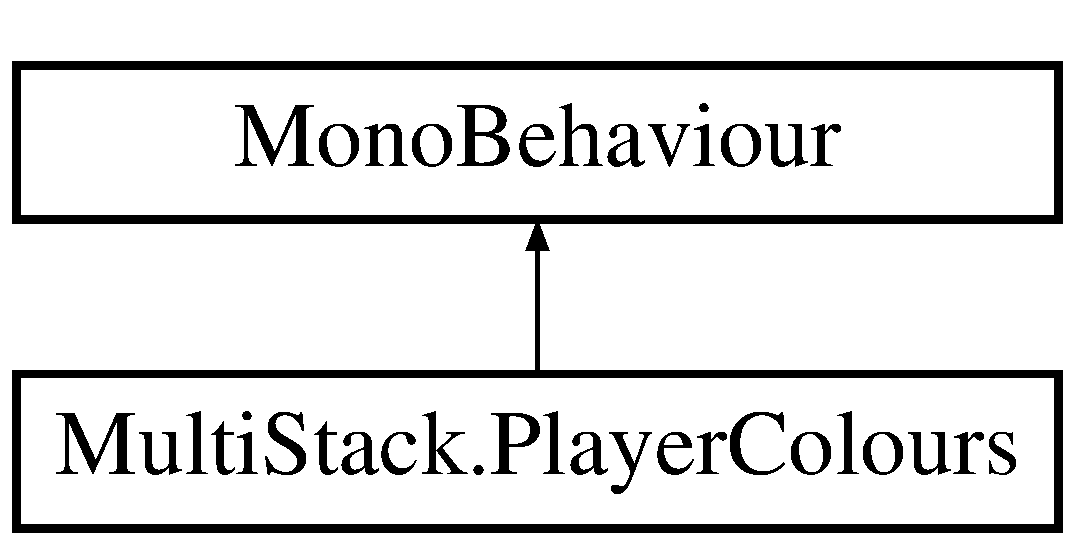
\includegraphics[height=2.000000cm]{class_multi_stack_1_1_player_colours}
\end{center}
\end{figure}
\subsection*{Public Attributes}
\begin{DoxyCompactItemize}
\item 
Color\mbox{[}$\,$\mbox{]} \hyperlink{class_multi_stack_1_1_player_colours_a3fdd21deb5bab6b7005ed9e72e2053a7}{colours}
\begin{DoxyCompactList}\small\item\em The colours for each player. \end{DoxyCompactList}\end{DoxyCompactItemize}


\subsection{Detailed Description}
Holds the coours for each player. 



\subsection{Member Data Documentation}
\hypertarget{class_multi_stack_1_1_player_colours_a3fdd21deb5bab6b7005ed9e72e2053a7}{}\index{Multi\+Stack\+::\+Player\+Colours@{Multi\+Stack\+::\+Player\+Colours}!colours@{colours}}
\index{colours@{colours}!Multi\+Stack\+::\+Player\+Colours@{Multi\+Stack\+::\+Player\+Colours}}
\subsubsection[{colours}]{\setlength{\rightskip}{0pt plus 5cm}Color \mbox{[}$\,$\mbox{]} Multi\+Stack.\+Player\+Colours.\+colours}\label{class_multi_stack_1_1_player_colours_a3fdd21deb5bab6b7005ed9e72e2053a7}


The colours for each player. 



The documentation for this class was generated from the following file\+:\begin{DoxyCompactItemize}
\item 
Multiplayer\+Stacker/\+Scripts/\+U\+I/Player\+Colours.\+cs\end{DoxyCompactItemize}

\hypertarget{class_multi_stack_1_1_player_number_count}{}\section{Multi\+Stack.\+Player\+Number\+Count Class Reference}
\label{class_multi_stack_1_1_player_number_count}\index{Multi\+Stack.\+Player\+Number\+Count@{Multi\+Stack.\+Player\+Number\+Count}}
Inheritance diagram for Multi\+Stack.\+Player\+Number\+Count\+:\begin{figure}[H]
\begin{center}
\leavevmode
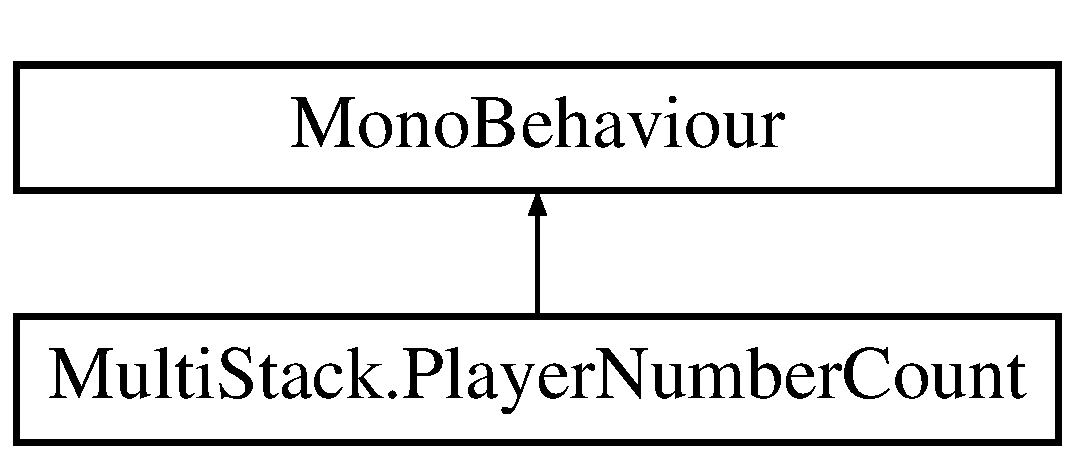
\includegraphics[height=2.000000cm]{class_multi_stack_1_1_player_number_count}
\end{center}
\end{figure}
\subsection*{Properties}
\begin{DoxyCompactItemize}
\item 
int \hyperlink{class_multi_stack_1_1_player_number_count_a39097aa99803f5dfc0e1c19283785d88}{number\+Of\+Players}\hspace{0.3cm}{\ttfamily  \mbox{[}get, set\mbox{]}}
\begin{DoxyCompactList}\small\item\em Gets or sets the number of players. Used to store the number of players between scenes. \end{DoxyCompactList}\end{DoxyCompactItemize}


\subsection{Property Documentation}
\hypertarget{class_multi_stack_1_1_player_number_count_a39097aa99803f5dfc0e1c19283785d88}{}\index{Multi\+Stack\+::\+Player\+Number\+Count@{Multi\+Stack\+::\+Player\+Number\+Count}!number\+Of\+Players@{number\+Of\+Players}}
\index{number\+Of\+Players@{number\+Of\+Players}!Multi\+Stack\+::\+Player\+Number\+Count@{Multi\+Stack\+::\+Player\+Number\+Count}}
\subsubsection[{number\+Of\+Players}]{\setlength{\rightskip}{0pt plus 5cm}int Multi\+Stack.\+Player\+Number\+Count.\+number\+Of\+Players\hspace{0.3cm}{\ttfamily [get]}, {\ttfamily [set]}}\label{class_multi_stack_1_1_player_number_count_a39097aa99803f5dfc0e1c19283785d88}


Gets or sets the number of players. Used to store the number of players between scenes. 

The number of players.

The documentation for this class was generated from the following file\+:\begin{DoxyCompactItemize}
\item 
Multiplayer\+Stacker/\+Scripts/Player\+Number\+Count.\+cs\end{DoxyCompactItemize}

\hypertarget{struct_multi_stack_1_1_player_physics_object}{}\section{Multi\+Stack.\+Player\+Physics\+Object Struct Reference}
\label{struct_multi_stack_1_1_player_physics_object}\index{Multi\+Stack.\+Player\+Physics\+Object@{Multi\+Stack.\+Player\+Physics\+Object}}


A structure defining a physics object.  


\subsection*{Public Attributes}
\begin{DoxyCompactItemize}
\item 
\hyperlink{namespace_multi_stack_ac7f637887fea673ceeae6fdd0598c048}{Shape} \hyperlink{struct_multi_stack_1_1_player_physics_object_a7232e0e0dce8cd41a4d60977c4c6bc7b}{shape}
\begin{DoxyCompactList}\small\item\em The type of shape this object represents. \end{DoxyCompactList}\item 
Game\+Object \hyperlink{struct_multi_stack_1_1_player_physics_object_a9ea1890efae7166e3f97e09034dfd505}{simple\+Prefab}
\begin{DoxyCompactList}\small\item\em A simple prefab without any of the associated scripts. When the shapes are being looped through and displayed at the beginning of a players turn the simple prefabs are used. \end{DoxyCompactList}\item 
Game\+Object \hyperlink{struct_multi_stack_1_1_player_physics_object_a12ec933050599f2b98759c1c4ceee830}{real\+Prefab}
\begin{DoxyCompactList}\small\item\em The real prefab. This is the prefab that is spawned once a shape has been selected. \end{DoxyCompactList}\item 
float \hyperlink{struct_multi_stack_1_1_player_physics_object_a19e58a0ebb90ee69437a21f12093e758}{weight}
\begin{DoxyCompactList}\small\item\em The chance that this object will spawn. The weight is proportional to other shapes weights. \end{DoxyCompactList}\end{DoxyCompactItemize}
\subsection*{Properties}
\begin{DoxyCompactItemize}
\item 
Game\+Object \hyperlink{struct_multi_stack_1_1_player_physics_object_ac4a840e0e27b4696fbbf7fbb105bd528}{instantiated\+Prefab}\hspace{0.3cm}{\ttfamily  \mbox{[}get, set\mbox{]}}
\begin{DoxyCompactList}\small\item\em Gets or sets the instantiated simple prefab. \end{DoxyCompactList}\end{DoxyCompactItemize}


\subsection{Detailed Description}
A structure defining a physics object. 



\subsection{Member Data Documentation}
\hypertarget{struct_multi_stack_1_1_player_physics_object_a12ec933050599f2b98759c1c4ceee830}{}\index{Multi\+Stack\+::\+Player\+Physics\+Object@{Multi\+Stack\+::\+Player\+Physics\+Object}!real\+Prefab@{real\+Prefab}}
\index{real\+Prefab@{real\+Prefab}!Multi\+Stack\+::\+Player\+Physics\+Object@{Multi\+Stack\+::\+Player\+Physics\+Object}}
\subsubsection[{real\+Prefab}]{\setlength{\rightskip}{0pt plus 5cm}Game\+Object Multi\+Stack.\+Player\+Physics\+Object.\+real\+Prefab}\label{struct_multi_stack_1_1_player_physics_object_a12ec933050599f2b98759c1c4ceee830}


The real prefab. This is the prefab that is spawned once a shape has been selected. 

\hypertarget{struct_multi_stack_1_1_player_physics_object_a7232e0e0dce8cd41a4d60977c4c6bc7b}{}\index{Multi\+Stack\+::\+Player\+Physics\+Object@{Multi\+Stack\+::\+Player\+Physics\+Object}!shape@{shape}}
\index{shape@{shape}!Multi\+Stack\+::\+Player\+Physics\+Object@{Multi\+Stack\+::\+Player\+Physics\+Object}}
\subsubsection[{shape}]{\setlength{\rightskip}{0pt plus 5cm}{\bf Shape} Multi\+Stack.\+Player\+Physics\+Object.\+shape}\label{struct_multi_stack_1_1_player_physics_object_a7232e0e0dce8cd41a4d60977c4c6bc7b}


The type of shape this object represents. 

\hypertarget{struct_multi_stack_1_1_player_physics_object_a9ea1890efae7166e3f97e09034dfd505}{}\index{Multi\+Stack\+::\+Player\+Physics\+Object@{Multi\+Stack\+::\+Player\+Physics\+Object}!simple\+Prefab@{simple\+Prefab}}
\index{simple\+Prefab@{simple\+Prefab}!Multi\+Stack\+::\+Player\+Physics\+Object@{Multi\+Stack\+::\+Player\+Physics\+Object}}
\subsubsection[{simple\+Prefab}]{\setlength{\rightskip}{0pt plus 5cm}Game\+Object Multi\+Stack.\+Player\+Physics\+Object.\+simple\+Prefab}\label{struct_multi_stack_1_1_player_physics_object_a9ea1890efae7166e3f97e09034dfd505}


A simple prefab without any of the associated scripts. When the shapes are being looped through and displayed at the beginning of a players turn the simple prefabs are used. 

\hypertarget{struct_multi_stack_1_1_player_physics_object_a19e58a0ebb90ee69437a21f12093e758}{}\index{Multi\+Stack\+::\+Player\+Physics\+Object@{Multi\+Stack\+::\+Player\+Physics\+Object}!weight@{weight}}
\index{weight@{weight}!Multi\+Stack\+::\+Player\+Physics\+Object@{Multi\+Stack\+::\+Player\+Physics\+Object}}
\subsubsection[{weight}]{\setlength{\rightskip}{0pt plus 5cm}float Multi\+Stack.\+Player\+Physics\+Object.\+weight}\label{struct_multi_stack_1_1_player_physics_object_a19e58a0ebb90ee69437a21f12093e758}


The chance that this object will spawn. The weight is proportional to other shapes weights. 



\subsection{Property Documentation}
\hypertarget{struct_multi_stack_1_1_player_physics_object_ac4a840e0e27b4696fbbf7fbb105bd528}{}\index{Multi\+Stack\+::\+Player\+Physics\+Object@{Multi\+Stack\+::\+Player\+Physics\+Object}!instantiated\+Prefab@{instantiated\+Prefab}}
\index{instantiated\+Prefab@{instantiated\+Prefab}!Multi\+Stack\+::\+Player\+Physics\+Object@{Multi\+Stack\+::\+Player\+Physics\+Object}}
\subsubsection[{instantiated\+Prefab}]{\setlength{\rightskip}{0pt plus 5cm}Game\+Object Multi\+Stack.\+Player\+Physics\+Object.\+instantiated\+Prefab\hspace{0.3cm}{\ttfamily [get]}, {\ttfamily [set]}}\label{struct_multi_stack_1_1_player_physics_object_ac4a840e0e27b4696fbbf7fbb105bd528}


Gets or sets the instantiated simple prefab. 

The instantiated prefab.

The documentation for this struct was generated from the following file\+:\begin{DoxyCompactItemize}
\item 
Multiplayer\+Stacker/\+Scripts/Player\+Physics\+Object.\+cs\end{DoxyCompactItemize}

\hypertarget{class_multi_stack_1_1_random_player_order_modifier}{}\section{Multi\+Stack.\+Random\+Player\+Order\+Modifier Class Reference}
\label{class_multi_stack_1_1_random_player_order_modifier}\index{Multi\+Stack.\+Random\+Player\+Order\+Modifier@{Multi\+Stack.\+Random\+Player\+Order\+Modifier}}


When enabled the order of players is randomised for this round.  


Inheritance diagram for Multi\+Stack.\+Random\+Player\+Order\+Modifier\+:\begin{figure}[H]
\begin{center}
\leavevmode
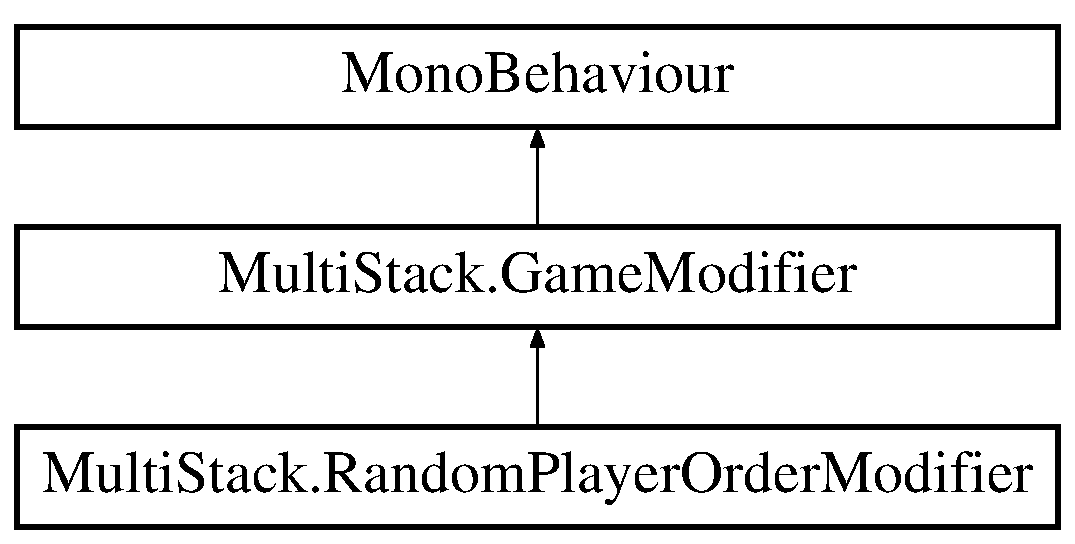
\includegraphics[height=3.000000cm]{class_multi_stack_1_1_random_player_order_modifier}
\end{center}
\end{figure}
\subsection*{Public Member Functions}
\begin{DoxyCompactItemize}
\item 
override void \hyperlink{class_multi_stack_1_1_random_player_order_modifier_a6f2965f6ee8933b1631974cefba9bd00}{Activate} ()
\begin{DoxyCompactList}\small\item\em Activate this modifier. Called at the beginning of the round. \end{DoxyCompactList}\item 
override void \hyperlink{class_multi_stack_1_1_random_player_order_modifier_a75341a38b55dde95e4037d5ce829ed72}{Deactivate} ()
\begin{DoxyCompactList}\small\item\em Deactivate this modifier. Called before a new modifier is enabled. \end{DoxyCompactList}\end{DoxyCompactItemize}
\subsection*{Additional Inherited Members}


\subsection{Detailed Description}
When enabled the order of players is randomised for this round. 



\subsection{Member Function Documentation}
\hypertarget{class_multi_stack_1_1_random_player_order_modifier_a6f2965f6ee8933b1631974cefba9bd00}{}\index{Multi\+Stack\+::\+Random\+Player\+Order\+Modifier@{Multi\+Stack\+::\+Random\+Player\+Order\+Modifier}!Activate@{Activate}}
\index{Activate@{Activate}!Multi\+Stack\+::\+Random\+Player\+Order\+Modifier@{Multi\+Stack\+::\+Random\+Player\+Order\+Modifier}}
\subsubsection[{Activate()}]{\setlength{\rightskip}{0pt plus 5cm}override void Multi\+Stack.\+Random\+Player\+Order\+Modifier.\+Activate (
\begin{DoxyParamCaption}
{}
\end{DoxyParamCaption}
)\hspace{0.3cm}{\ttfamily [virtual]}}\label{class_multi_stack_1_1_random_player_order_modifier_a6f2965f6ee8933b1631974cefba9bd00}


Activate this modifier. Called at the beginning of the round. 



Implements \hyperlink{class_multi_stack_1_1_game_modifier_a3fb880f9728f8680bf473ac5c7f6832e}{Multi\+Stack.\+Game\+Modifier}.

\hypertarget{class_multi_stack_1_1_random_player_order_modifier_a75341a38b55dde95e4037d5ce829ed72}{}\index{Multi\+Stack\+::\+Random\+Player\+Order\+Modifier@{Multi\+Stack\+::\+Random\+Player\+Order\+Modifier}!Deactivate@{Deactivate}}
\index{Deactivate@{Deactivate}!Multi\+Stack\+::\+Random\+Player\+Order\+Modifier@{Multi\+Stack\+::\+Random\+Player\+Order\+Modifier}}
\subsubsection[{Deactivate()}]{\setlength{\rightskip}{0pt plus 5cm}override void Multi\+Stack.\+Random\+Player\+Order\+Modifier.\+Deactivate (
\begin{DoxyParamCaption}
{}
\end{DoxyParamCaption}
)\hspace{0.3cm}{\ttfamily [virtual]}}\label{class_multi_stack_1_1_random_player_order_modifier_a75341a38b55dde95e4037d5ce829ed72}


Deactivate this modifier. Called before a new modifier is enabled. 



Implements \hyperlink{class_multi_stack_1_1_game_modifier_abe04db6ab31f5e5063739d8e5a3f7ad1}{Multi\+Stack.\+Game\+Modifier}.



The documentation for this class was generated from the following file\+:\begin{DoxyCompactItemize}
\item 
Multiplayer\+Stacker/\+Scripts/\+Modifiers/Random\+Player\+Order\+Modifier.\+cs\end{DoxyCompactItemize}

\hypertarget{class_multi_stack_1_1_reverse_drag_modifier}{}\section{Multi\+Stack.\+Reverse\+Drag\+Modifier Class Reference}
\label{class_multi_stack_1_1_reverse_drag_modifier}\index{Multi\+Stack.\+Reverse\+Drag\+Modifier@{Multi\+Stack.\+Reverse\+Drag\+Modifier}}


When enabled drag is reversed e.\+g. when the player drags the mouse/finger left the shape moves right.  


Inheritance diagram for Multi\+Stack.\+Reverse\+Drag\+Modifier\+:\begin{figure}[H]
\begin{center}
\leavevmode
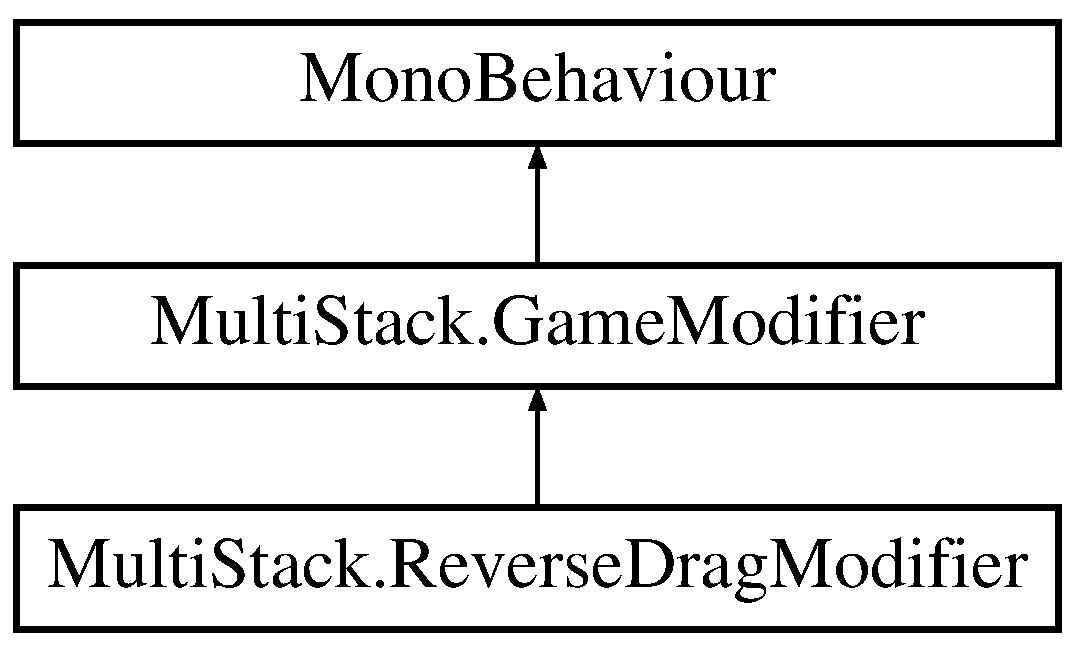
\includegraphics[height=3.000000cm]{class_multi_stack_1_1_reverse_drag_modifier}
\end{center}
\end{figure}
\subsection*{Public Member Functions}
\begin{DoxyCompactItemize}
\item 
override void \hyperlink{class_multi_stack_1_1_reverse_drag_modifier_a4210fbc0eb598a7b4f31976407e4e1ff}{Activate} ()
\begin{DoxyCompactList}\small\item\em Activate this modifier. Called at the beginning of the round. \end{DoxyCompactList}\item 
override void \hyperlink{class_multi_stack_1_1_reverse_drag_modifier_a32d5963443ed0867c51c97f76128d3ec}{Deactivate} ()
\begin{DoxyCompactList}\small\item\em Deactivate this modifier. Called before a new modifier is enabled. \end{DoxyCompactList}\end{DoxyCompactItemize}
\subsection*{Public Attributes}
\begin{DoxyCompactItemize}
\item 
\hypertarget{class_multi_stack_1_1_reverse_drag_modifier_a683166c961dfdb5f7eeed6fa2b5d0379}{}\hyperlink{class_multi_stack_1_1_click_handler}{Click\+Handler} {\bfseries click\+Handler}\label{class_multi_stack_1_1_reverse_drag_modifier_a683166c961dfdb5f7eeed6fa2b5d0379}

\end{DoxyCompactItemize}


\subsection{Detailed Description}
When enabled drag is reversed e.\+g. when the player drags the mouse/finger left the shape moves right. 



\subsection{Member Function Documentation}
\hypertarget{class_multi_stack_1_1_reverse_drag_modifier_a4210fbc0eb598a7b4f31976407e4e1ff}{}\index{Multi\+Stack\+::\+Reverse\+Drag\+Modifier@{Multi\+Stack\+::\+Reverse\+Drag\+Modifier}!Activate@{Activate}}
\index{Activate@{Activate}!Multi\+Stack\+::\+Reverse\+Drag\+Modifier@{Multi\+Stack\+::\+Reverse\+Drag\+Modifier}}
\subsubsection[{Activate()}]{\setlength{\rightskip}{0pt plus 5cm}override void Multi\+Stack.\+Reverse\+Drag\+Modifier.\+Activate (
\begin{DoxyParamCaption}
{}
\end{DoxyParamCaption}
)\hspace{0.3cm}{\ttfamily [virtual]}}\label{class_multi_stack_1_1_reverse_drag_modifier_a4210fbc0eb598a7b4f31976407e4e1ff}


Activate this modifier. Called at the beginning of the round. 



Implements \hyperlink{class_multi_stack_1_1_game_modifier_a3fb880f9728f8680bf473ac5c7f6832e}{Multi\+Stack.\+Game\+Modifier}.

\hypertarget{class_multi_stack_1_1_reverse_drag_modifier_a32d5963443ed0867c51c97f76128d3ec}{}\index{Multi\+Stack\+::\+Reverse\+Drag\+Modifier@{Multi\+Stack\+::\+Reverse\+Drag\+Modifier}!Deactivate@{Deactivate}}
\index{Deactivate@{Deactivate}!Multi\+Stack\+::\+Reverse\+Drag\+Modifier@{Multi\+Stack\+::\+Reverse\+Drag\+Modifier}}
\subsubsection[{Deactivate()}]{\setlength{\rightskip}{0pt plus 5cm}override void Multi\+Stack.\+Reverse\+Drag\+Modifier.\+Deactivate (
\begin{DoxyParamCaption}
{}
\end{DoxyParamCaption}
)\hspace{0.3cm}{\ttfamily [virtual]}}\label{class_multi_stack_1_1_reverse_drag_modifier_a32d5963443ed0867c51c97f76128d3ec}


Deactivate this modifier. Called before a new modifier is enabled. 



Implements \hyperlink{class_multi_stack_1_1_game_modifier_abe04db6ab31f5e5063739d8e5a3f7ad1}{Multi\+Stack.\+Game\+Modifier}.



The documentation for this class was generated from the following file\+:\begin{DoxyCompactItemize}
\item 
Multiplayer\+Stacker/\+Scripts/\+Modifiers/Reverse\+Drag\+Modifier.\+cs\end{DoxyCompactItemize}

\hypertarget{class_multi_stack_1_1_score_data}{}\section{Multi\+Stack.\+Score\+Data Class Reference}
\label{class_multi_stack_1_1_score_data}\index{Multi\+Stack.\+Score\+Data@{Multi\+Stack.\+Score\+Data}}


Class to store serializable height/round data.  


\subsection*{Public Member Functions}
\begin{DoxyCompactItemize}
\item 
\hypertarget{class_multi_stack_1_1_score_data_a31a1224f670eee65b8d5bb4c17dd3f7f}{}{\bfseries Score\+Data} (int height, int round)\label{class_multi_stack_1_1_score_data_a31a1224f670eee65b8d5bb4c17dd3f7f}

\end{DoxyCompactItemize}
\subsection*{Properties}
\begin{DoxyCompactItemize}
\item 
\hypertarget{class_multi_stack_1_1_score_data_a1bcafbbbac6cd706b9fcd43bd9f24ff5}{}int {\bfseries height}\hspace{0.3cm}{\ttfamily  \mbox{[}get\mbox{]}}\label{class_multi_stack_1_1_score_data_a1bcafbbbac6cd706b9fcd43bd9f24ff5}

\item 
\hypertarget{class_multi_stack_1_1_score_data_a2cb31be34c6c2aaa90027384b7be6390}{}int {\bfseries round}\hspace{0.3cm}{\ttfamily  \mbox{[}get\mbox{]}}\label{class_multi_stack_1_1_score_data_a2cb31be34c6c2aaa90027384b7be6390}

\end{DoxyCompactItemize}


\subsection{Detailed Description}
Class to store serializable height/round data. 



The documentation for this class was generated from the following file\+:\begin{DoxyCompactItemize}
\item 
Multiplayer\+Stacker/\+Scripts/\+High Score/Data\+Persistence.\+cs\end{DoxyCompactItemize}

\hypertarget{class_multi_stack_1_1_shakey_shapes_modifier}{}\section{Multi\+Stack.\+Shakey\+Shapes\+Modifier Class Reference}
\label{class_multi_stack_1_1_shakey_shapes_modifier}\index{Multi\+Stack.\+Shakey\+Shapes\+Modifier@{Multi\+Stack.\+Shakey\+Shapes\+Modifier}}


When enabled a random offset is added to a dragged shape each timestep.  


Inheritance diagram for Multi\+Stack.\+Shakey\+Shapes\+Modifier\+:\begin{figure}[H]
\begin{center}
\leavevmode
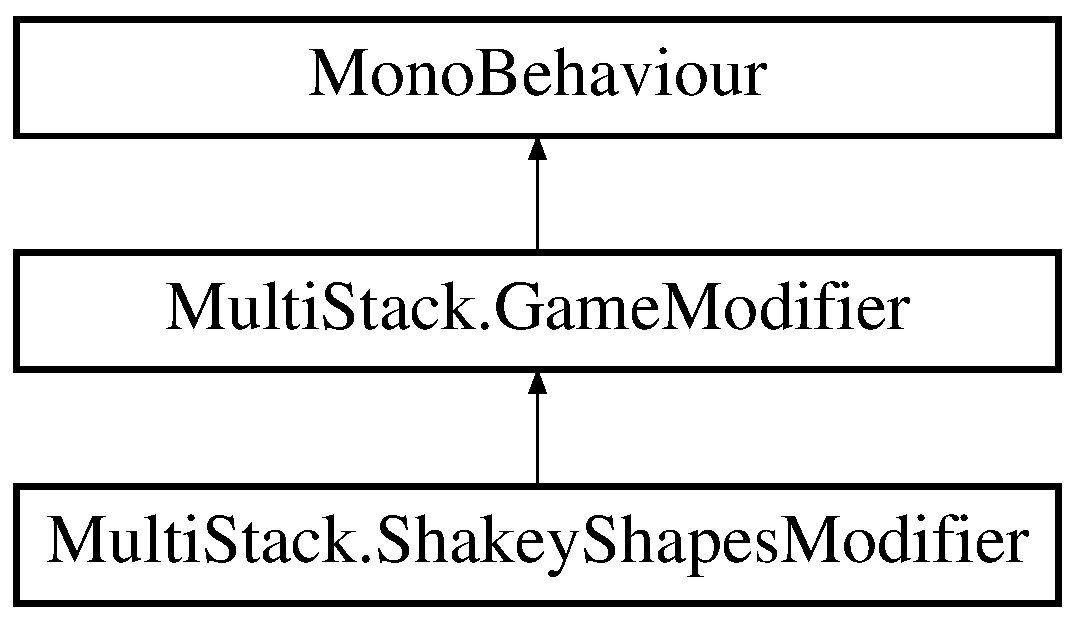
\includegraphics[height=3.000000cm]{class_multi_stack_1_1_shakey_shapes_modifier}
\end{center}
\end{figure}
\subsection*{Public Member Functions}
\begin{DoxyCompactItemize}
\item 
override void \hyperlink{class_multi_stack_1_1_shakey_shapes_modifier_ae45e7bdf85d9655ef28b5a33e0ae72e6}{Activate} ()
\begin{DoxyCompactList}\small\item\em Activate this modifier. Called at the beginning of the round. \end{DoxyCompactList}\item 
override void \hyperlink{class_multi_stack_1_1_shakey_shapes_modifier_a10f32463b2e5e38d7b50698232e145b4}{Deactivate} ()
\begin{DoxyCompactList}\small\item\em Deactivate this modifier. Called before a new modifier is enabled. \end{DoxyCompactList}\end{DoxyCompactItemize}
\subsection*{Public Attributes}
\begin{DoxyCompactItemize}
\item 
\hypertarget{class_multi_stack_1_1_shakey_shapes_modifier_a691fc53b2d5c01ae6ca303480ea4c1ff}{}\hyperlink{class_multi_stack_1_1_click_handler}{Click\+Handler} {\bfseries click\+Handler}\label{class_multi_stack_1_1_shakey_shapes_modifier_a691fc53b2d5c01ae6ca303480ea4c1ff}

\end{DoxyCompactItemize}


\subsection{Detailed Description}
When enabled a random offset is added to a dragged shape each timestep. 



\subsection{Member Function Documentation}
\hypertarget{class_multi_stack_1_1_shakey_shapes_modifier_ae45e7bdf85d9655ef28b5a33e0ae72e6}{}\index{Multi\+Stack\+::\+Shakey\+Shapes\+Modifier@{Multi\+Stack\+::\+Shakey\+Shapes\+Modifier}!Activate@{Activate}}
\index{Activate@{Activate}!Multi\+Stack\+::\+Shakey\+Shapes\+Modifier@{Multi\+Stack\+::\+Shakey\+Shapes\+Modifier}}
\subsubsection[{Activate()}]{\setlength{\rightskip}{0pt plus 5cm}override void Multi\+Stack.\+Shakey\+Shapes\+Modifier.\+Activate (
\begin{DoxyParamCaption}
{}
\end{DoxyParamCaption}
)\hspace{0.3cm}{\ttfamily [virtual]}}\label{class_multi_stack_1_1_shakey_shapes_modifier_ae45e7bdf85d9655ef28b5a33e0ae72e6}


Activate this modifier. Called at the beginning of the round. 



Implements \hyperlink{class_multi_stack_1_1_game_modifier_a3fb880f9728f8680bf473ac5c7f6832e}{Multi\+Stack.\+Game\+Modifier}.

\hypertarget{class_multi_stack_1_1_shakey_shapes_modifier_a10f32463b2e5e38d7b50698232e145b4}{}\index{Multi\+Stack\+::\+Shakey\+Shapes\+Modifier@{Multi\+Stack\+::\+Shakey\+Shapes\+Modifier}!Deactivate@{Deactivate}}
\index{Deactivate@{Deactivate}!Multi\+Stack\+::\+Shakey\+Shapes\+Modifier@{Multi\+Stack\+::\+Shakey\+Shapes\+Modifier}}
\subsubsection[{Deactivate()}]{\setlength{\rightskip}{0pt plus 5cm}override void Multi\+Stack.\+Shakey\+Shapes\+Modifier.\+Deactivate (
\begin{DoxyParamCaption}
{}
\end{DoxyParamCaption}
)\hspace{0.3cm}{\ttfamily [virtual]}}\label{class_multi_stack_1_1_shakey_shapes_modifier_a10f32463b2e5e38d7b50698232e145b4}


Deactivate this modifier. Called before a new modifier is enabled. 



Implements \hyperlink{class_multi_stack_1_1_game_modifier_abe04db6ab31f5e5063739d8e5a3f7ad1}{Multi\+Stack.\+Game\+Modifier}.



The documentation for this class was generated from the following file\+:\begin{DoxyCompactItemize}
\item 
Multiplayer\+Stacker/\+Scripts/\+Modifiers/Shakey\+Shapes\+Modifier.\+cs\end{DoxyCompactItemize}

\hypertarget{class_multi_stack_1_1_shape_movement_speed_modifier}{}\section{Multi\+Stack.\+Shape\+Movement\+Speed\+Modifier Class Reference}
\label{class_multi_stack_1_1_shape_movement_speed_modifier}\index{Multi\+Stack.\+Shape\+Movement\+Speed\+Modifier@{Multi\+Stack.\+Shape\+Movement\+Speed\+Modifier}}


When enabled the drag speed is changed to Multi\+Stack.\+Shape\+Movement\+Speed\+Modifier.\+shape\+Movement\+Speed.  


Inheritance diagram for Multi\+Stack.\+Shape\+Movement\+Speed\+Modifier\+:\begin{figure}[H]
\begin{center}
\leavevmode
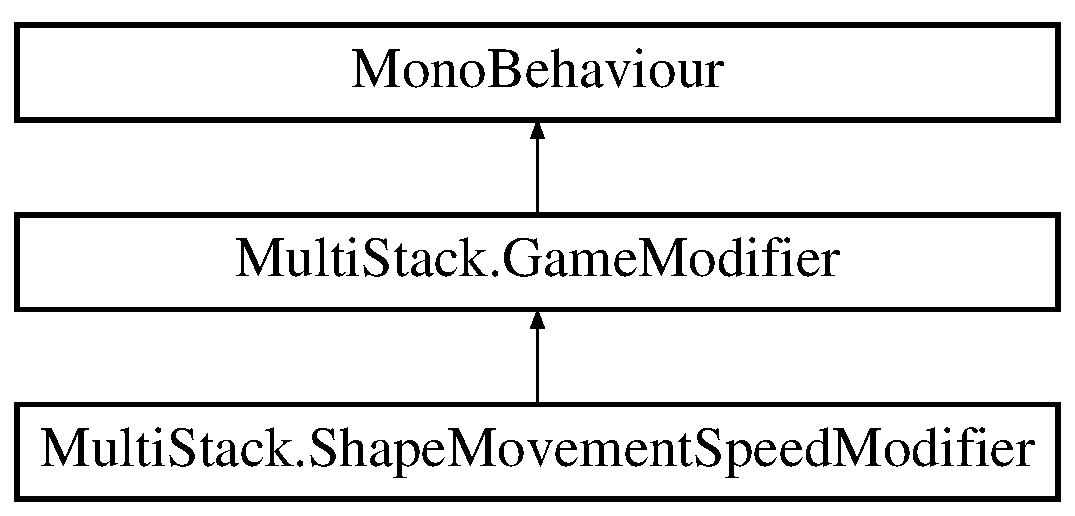
\includegraphics[height=3.000000cm]{class_multi_stack_1_1_shape_movement_speed_modifier}
\end{center}
\end{figure}
\subsection*{Public Member Functions}
\begin{DoxyCompactItemize}
\item 
override void \hyperlink{class_multi_stack_1_1_shape_movement_speed_modifier_a9c340894f491f8b11b8753bb4f333d4c}{Activate} ()
\begin{DoxyCompactList}\small\item\em Activate this modifier. Called at the beginning of the round. \end{DoxyCompactList}\item 
override void \hyperlink{class_multi_stack_1_1_shape_movement_speed_modifier_a6c8209e8db355d3b3204167c76049503}{Deactivate} ()
\begin{DoxyCompactList}\small\item\em Deactivate this modifier. Called before a new modifier is enabled. \end{DoxyCompactList}\end{DoxyCompactItemize}
\subsection*{Public Attributes}
\begin{DoxyCompactItemize}
\item 
\hypertarget{class_multi_stack_1_1_shape_movement_speed_modifier_aa696b8932977f88c8d41d6fc303fd5be}{}\hyperlink{class_multi_stack_1_1_click_handler}{Click\+Handler} {\bfseries click\+Handler}\label{class_multi_stack_1_1_shape_movement_speed_modifier_aa696b8932977f88c8d41d6fc303fd5be}

\item 
\hypertarget{class_multi_stack_1_1_shape_movement_speed_modifier_a41ec729fc14c8f457b24824f4825fc4c}{}float {\bfseries shape\+Movement\+Speed}\label{class_multi_stack_1_1_shape_movement_speed_modifier_a41ec729fc14c8f457b24824f4825fc4c}

\end{DoxyCompactItemize}


\subsection{Detailed Description}
When enabled the drag speed is changed to Multi\+Stack.\+Shape\+Movement\+Speed\+Modifier.\+shape\+Movement\+Speed. 



\subsection{Member Function Documentation}
\hypertarget{class_multi_stack_1_1_shape_movement_speed_modifier_a9c340894f491f8b11b8753bb4f333d4c}{}\index{Multi\+Stack\+::\+Shape\+Movement\+Speed\+Modifier@{Multi\+Stack\+::\+Shape\+Movement\+Speed\+Modifier}!Activate@{Activate}}
\index{Activate@{Activate}!Multi\+Stack\+::\+Shape\+Movement\+Speed\+Modifier@{Multi\+Stack\+::\+Shape\+Movement\+Speed\+Modifier}}
\subsubsection[{Activate()}]{\setlength{\rightskip}{0pt plus 5cm}override void Multi\+Stack.\+Shape\+Movement\+Speed\+Modifier.\+Activate (
\begin{DoxyParamCaption}
{}
\end{DoxyParamCaption}
)\hspace{0.3cm}{\ttfamily [virtual]}}\label{class_multi_stack_1_1_shape_movement_speed_modifier_a9c340894f491f8b11b8753bb4f333d4c}


Activate this modifier. Called at the beginning of the round. 



Implements \hyperlink{class_multi_stack_1_1_game_modifier_a3fb880f9728f8680bf473ac5c7f6832e}{Multi\+Stack.\+Game\+Modifier}.

\hypertarget{class_multi_stack_1_1_shape_movement_speed_modifier_a6c8209e8db355d3b3204167c76049503}{}\index{Multi\+Stack\+::\+Shape\+Movement\+Speed\+Modifier@{Multi\+Stack\+::\+Shape\+Movement\+Speed\+Modifier}!Deactivate@{Deactivate}}
\index{Deactivate@{Deactivate}!Multi\+Stack\+::\+Shape\+Movement\+Speed\+Modifier@{Multi\+Stack\+::\+Shape\+Movement\+Speed\+Modifier}}
\subsubsection[{Deactivate()}]{\setlength{\rightskip}{0pt plus 5cm}override void Multi\+Stack.\+Shape\+Movement\+Speed\+Modifier.\+Deactivate (
\begin{DoxyParamCaption}
{}
\end{DoxyParamCaption}
)\hspace{0.3cm}{\ttfamily [virtual]}}\label{class_multi_stack_1_1_shape_movement_speed_modifier_a6c8209e8db355d3b3204167c76049503}


Deactivate this modifier. Called before a new modifier is enabled. 



Implements \hyperlink{class_multi_stack_1_1_game_modifier_abe04db6ab31f5e5063739d8e5a3f7ad1}{Multi\+Stack.\+Game\+Modifier}.



The documentation for this class was generated from the following file\+:\begin{DoxyCompactItemize}
\item 
Multiplayer\+Stacker/\+Scripts/\+Modifiers/Shape\+Movement\+Speed\+Modifier.\+cs\end{DoxyCompactItemize}

\hypertarget{class_multi_stack_1_1_shape_size_modifier}{}\section{Multi\+Stack.\+Shape\+Size\+Modifier Class Reference}
\label{class_multi_stack_1_1_shape_size_modifier}\index{Multi\+Stack.\+Shape\+Size\+Modifier@{Multi\+Stack.\+Shape\+Size\+Modifier}}


When enabled all newly spawned shapes size is multiplied by Multi\+Stack.\+Shape\+Size\+Modifier.\+size\+Modifier.  


Inheritance diagram for Multi\+Stack.\+Shape\+Size\+Modifier\+:\begin{figure}[H]
\begin{center}
\leavevmode
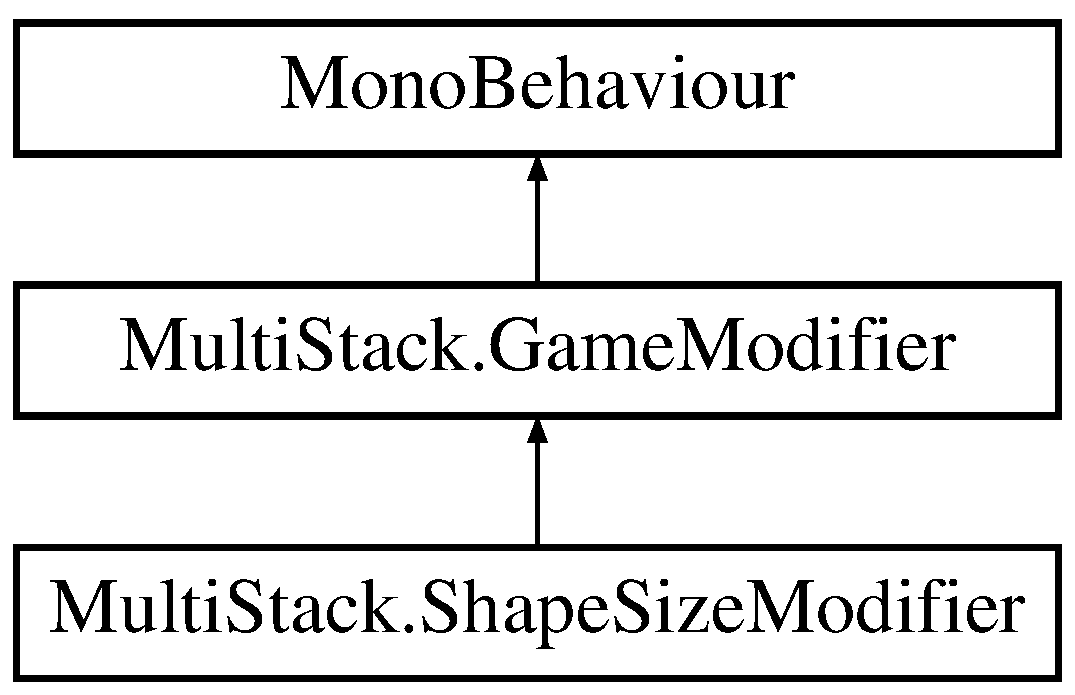
\includegraphics[height=3.000000cm]{class_multi_stack_1_1_shape_size_modifier}
\end{center}
\end{figure}
\subsection*{Public Member Functions}
\begin{DoxyCompactItemize}
\item 
override void \hyperlink{class_multi_stack_1_1_shape_size_modifier_a5dd27bb25d63f05f2d6c1f4c4f88fd3f}{Activate} ()
\begin{DoxyCompactList}\small\item\em Activate this modifier. Called at the beginning of the round. \end{DoxyCompactList}\item 
override void \hyperlink{class_multi_stack_1_1_shape_size_modifier_a74e6cc4af581e1167679d0b3d9740785}{Deactivate} ()
\begin{DoxyCompactList}\small\item\em Deactivate this modifier. Called before a new modifier is enabled. \end{DoxyCompactList}\end{DoxyCompactItemize}
\subsection*{Public Attributes}
\begin{DoxyCompactItemize}
\item 
\hypertarget{class_multi_stack_1_1_shape_size_modifier_ad1b3c3fd79bfc2ed70f471d73c983749}{}float {\bfseries size\+Modifier}\label{class_multi_stack_1_1_shape_size_modifier_ad1b3c3fd79bfc2ed70f471d73c983749}

\end{DoxyCompactItemize}


\subsection{Detailed Description}
When enabled all newly spawned shapes size is multiplied by Multi\+Stack.\+Shape\+Size\+Modifier.\+size\+Modifier. 



\subsection{Member Function Documentation}
\hypertarget{class_multi_stack_1_1_shape_size_modifier_a5dd27bb25d63f05f2d6c1f4c4f88fd3f}{}\index{Multi\+Stack\+::\+Shape\+Size\+Modifier@{Multi\+Stack\+::\+Shape\+Size\+Modifier}!Activate@{Activate}}
\index{Activate@{Activate}!Multi\+Stack\+::\+Shape\+Size\+Modifier@{Multi\+Stack\+::\+Shape\+Size\+Modifier}}
\subsubsection[{Activate()}]{\setlength{\rightskip}{0pt plus 5cm}override void Multi\+Stack.\+Shape\+Size\+Modifier.\+Activate (
\begin{DoxyParamCaption}
{}
\end{DoxyParamCaption}
)\hspace{0.3cm}{\ttfamily [virtual]}}\label{class_multi_stack_1_1_shape_size_modifier_a5dd27bb25d63f05f2d6c1f4c4f88fd3f}


Activate this modifier. Called at the beginning of the round. 



Implements \hyperlink{class_multi_stack_1_1_game_modifier_a3fb880f9728f8680bf473ac5c7f6832e}{Multi\+Stack.\+Game\+Modifier}.

\hypertarget{class_multi_stack_1_1_shape_size_modifier_a74e6cc4af581e1167679d0b3d9740785}{}\index{Multi\+Stack\+::\+Shape\+Size\+Modifier@{Multi\+Stack\+::\+Shape\+Size\+Modifier}!Deactivate@{Deactivate}}
\index{Deactivate@{Deactivate}!Multi\+Stack\+::\+Shape\+Size\+Modifier@{Multi\+Stack\+::\+Shape\+Size\+Modifier}}
\subsubsection[{Deactivate()}]{\setlength{\rightskip}{0pt plus 5cm}override void Multi\+Stack.\+Shape\+Size\+Modifier.\+Deactivate (
\begin{DoxyParamCaption}
{}
\end{DoxyParamCaption}
)\hspace{0.3cm}{\ttfamily [virtual]}}\label{class_multi_stack_1_1_shape_size_modifier_a74e6cc4af581e1167679d0b3d9740785}


Deactivate this modifier. Called before a new modifier is enabled. 



Implements \hyperlink{class_multi_stack_1_1_game_modifier_abe04db6ab31f5e5063739d8e5a3f7ad1}{Multi\+Stack.\+Game\+Modifier}.



The documentation for this class was generated from the following file\+:\begin{DoxyCompactItemize}
\item 
Multiplayer\+Stacker/\+Scripts/\+Modifiers/Shape\+Size\+Modifier.\+cs\end{DoxyCompactItemize}

\hypertarget{class_multi_stack_1_1_spring_modifier}{}\section{Multi\+Stack.\+Spring\+Modifier Class Reference}
\label{class_multi_stack_1_1_spring_modifier}\index{Multi\+Stack.\+Spring\+Modifier@{Multi\+Stack.\+Spring\+Modifier}}


When enabled the shapes are attached to springs when being dragged. This results in a harder to control shape.  


Inheritance diagram for Multi\+Stack.\+Spring\+Modifier\+:\begin{figure}[H]
\begin{center}
\leavevmode
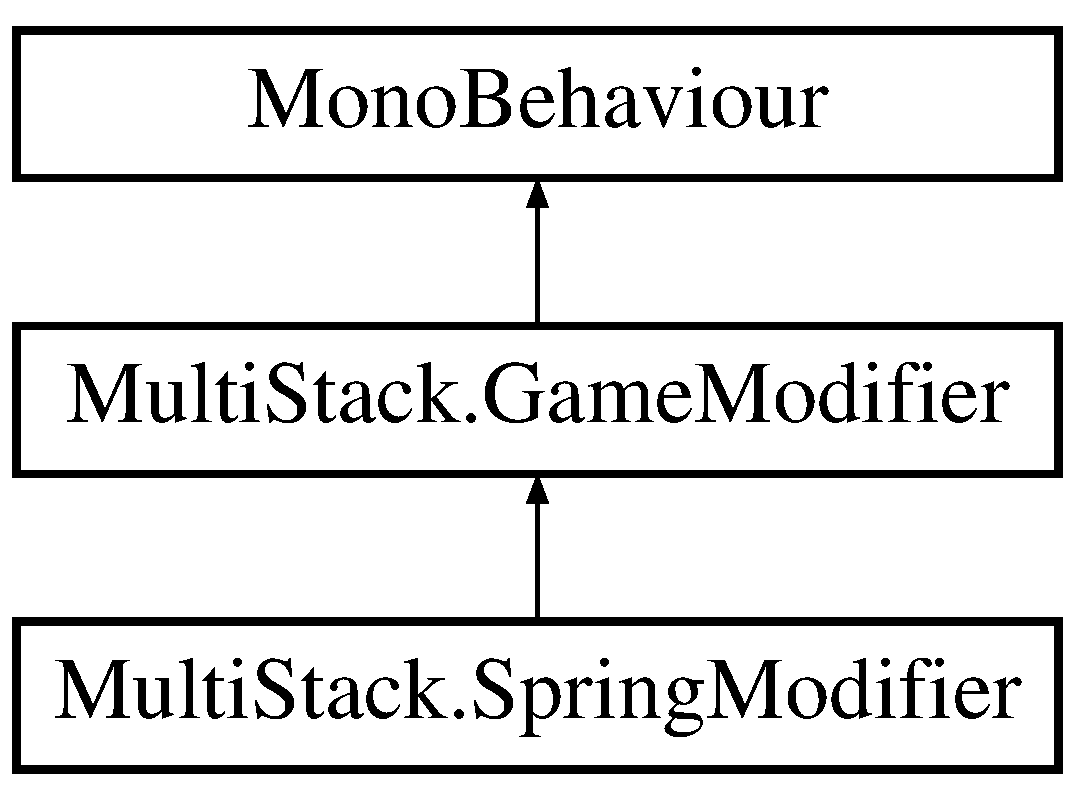
\includegraphics[height=3.000000cm]{class_multi_stack_1_1_spring_modifier}
\end{center}
\end{figure}
\subsection*{Public Member Functions}
\begin{DoxyCompactItemize}
\item 
override void \hyperlink{class_multi_stack_1_1_spring_modifier_ac96460f57d038035461804282c110040}{Activate} ()
\begin{DoxyCompactList}\small\item\em Activate this modifier. Called at the beginning of the round. \end{DoxyCompactList}\item 
override void \hyperlink{class_multi_stack_1_1_spring_modifier_ae6aaf8c2806a1c844b1700977efb2dbc}{Deactivate} ()
\begin{DoxyCompactList}\small\item\em Deactivate this modifier. Called before a new modifier is enabled. \end{DoxyCompactList}\end{DoxyCompactItemize}
\subsection*{Public Attributes}
\begin{DoxyCompactItemize}
\item 
\hypertarget{class_multi_stack_1_1_spring_modifier_a365b9a4fe8ad8e9d999eb434e076efa9}{}\hyperlink{class_multi_stack_1_1_click_handler}{Click\+Handler} {\bfseries click\+Handler}\label{class_multi_stack_1_1_spring_modifier_a365b9a4fe8ad8e9d999eb434e076efa9}

\end{DoxyCompactItemize}


\subsection{Detailed Description}
When enabled the shapes are attached to springs when being dragged. This results in a harder to control shape. 



\subsection{Member Function Documentation}
\hypertarget{class_multi_stack_1_1_spring_modifier_ac96460f57d038035461804282c110040}{}\index{Multi\+Stack\+::\+Spring\+Modifier@{Multi\+Stack\+::\+Spring\+Modifier}!Activate@{Activate}}
\index{Activate@{Activate}!Multi\+Stack\+::\+Spring\+Modifier@{Multi\+Stack\+::\+Spring\+Modifier}}
\subsubsection[{Activate()}]{\setlength{\rightskip}{0pt plus 5cm}override void Multi\+Stack.\+Spring\+Modifier.\+Activate (
\begin{DoxyParamCaption}
{}
\end{DoxyParamCaption}
)\hspace{0.3cm}{\ttfamily [virtual]}}\label{class_multi_stack_1_1_spring_modifier_ac96460f57d038035461804282c110040}


Activate this modifier. Called at the beginning of the round. 



Implements \hyperlink{class_multi_stack_1_1_game_modifier_a3fb880f9728f8680bf473ac5c7f6832e}{Multi\+Stack.\+Game\+Modifier}.

\hypertarget{class_multi_stack_1_1_spring_modifier_ae6aaf8c2806a1c844b1700977efb2dbc}{}\index{Multi\+Stack\+::\+Spring\+Modifier@{Multi\+Stack\+::\+Spring\+Modifier}!Deactivate@{Deactivate}}
\index{Deactivate@{Deactivate}!Multi\+Stack\+::\+Spring\+Modifier@{Multi\+Stack\+::\+Spring\+Modifier}}
\subsubsection[{Deactivate()}]{\setlength{\rightskip}{0pt plus 5cm}override void Multi\+Stack.\+Spring\+Modifier.\+Deactivate (
\begin{DoxyParamCaption}
{}
\end{DoxyParamCaption}
)\hspace{0.3cm}{\ttfamily [virtual]}}\label{class_multi_stack_1_1_spring_modifier_ae6aaf8c2806a1c844b1700977efb2dbc}


Deactivate this modifier. Called before a new modifier is enabled. 



Implements \hyperlink{class_multi_stack_1_1_game_modifier_abe04db6ab31f5e5063739d8e5a3f7ad1}{Multi\+Stack.\+Game\+Modifier}.



The documentation for this class was generated from the following file\+:\begin{DoxyCompactItemize}
\item 
Multiplayer\+Stacker/\+Scripts/\+Modifiers/Spring\+Modifier.\+cs\end{DoxyCompactItemize}

\hypertarget{class_multi_stack_1_1_stage_selector}{}\section{Multi\+Stack.\+Stage\+Selector Class Reference}
\label{class_multi_stack_1_1_stage_selector}\index{Multi\+Stack.\+Stage\+Selector@{Multi\+Stack.\+Stage\+Selector}}


Used to select a stage for the game. A random stage is selected at the beginning of each game.  


Inheritance diagram for Multi\+Stack.\+Stage\+Selector\+:\begin{figure}[H]
\begin{center}
\leavevmode
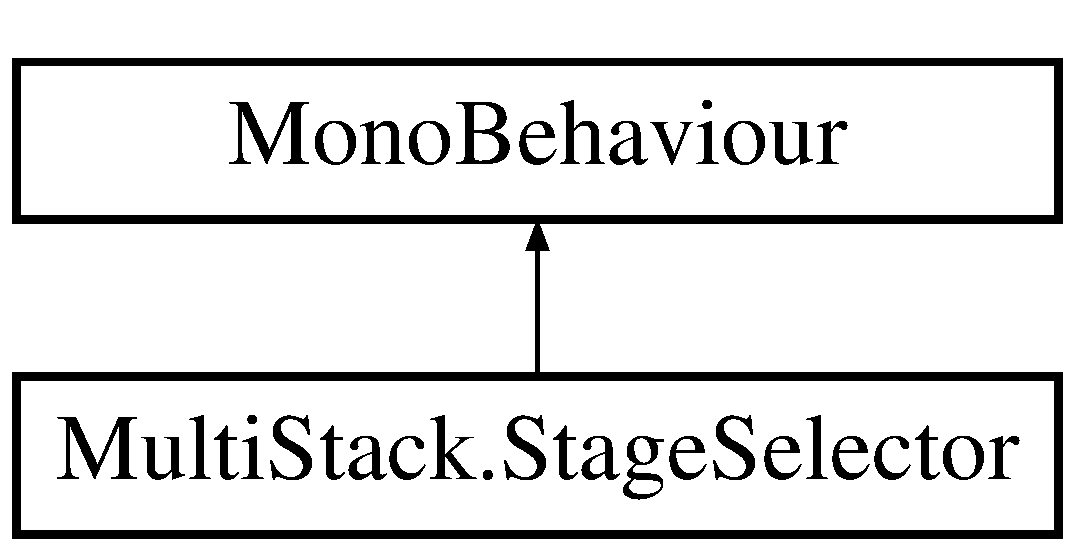
\includegraphics[height=2.000000cm]{class_multi_stack_1_1_stage_selector}
\end{center}
\end{figure}
\subsection*{Public Member Functions}
\begin{DoxyCompactItemize}
\item 
void \hyperlink{class_multi_stack_1_1_stage_selector_aca29f790cecb0ac7e2b6244ac0d1a6c9}{Call\+Back\+On\+Stage\+Complete} (\hyperlink{namespace_multi_stack_a4bd4097b52deebcafccf5815a8495960}{Call\+Back} call\+Back)
\begin{DoxyCompactList}\small\item\em Injects a method to be invoked when the stage spawn has completed. \end{DoxyCompactList}\item 
void \hyperlink{class_multi_stack_1_1_stage_selector_abee538fc62118823508d31ebff5a68d0}{Spawn\+Stage} ()
\begin{DoxyCompactList}\small\item\em Begins the stage spawning process. Updates the U\+I with \hyperlink{class_multi_stack_1_1_stage_selector_a199ae7412400d6e934dba1d2dc6b4f45}{Multi\+Stack.\+Stage\+Selector.\+stage\+Text}, loops through the stages and spawns the final stage. Invokes callback method set by \hyperlink{class_multi_stack_1_1_stage_selector_aca29f790cecb0ac7e2b6244ac0d1a6c9}{Multi\+Stack.\+Stage\+Selector.\+Call\+Back\+On\+Stage\+Complete} if present. \end{DoxyCompactList}\end{DoxyCompactItemize}
\subsection*{Public Attributes}
\begin{DoxyCompactItemize}
\item 
\hyperlink{class_multi_stack_1_1_game_text}{Game\+Text} \hyperlink{class_multi_stack_1_1_stage_selector_a6f837e9ba7fc2d949f2d36ef97159835}{info\+Text}
\begin{DoxyCompactList}\small\item\em Used to display a message at the beginning of the stage spawn process. \end{DoxyCompactList}\item 
string \hyperlink{class_multi_stack_1_1_stage_selector_a199ae7412400d6e934dba1d2dc6b4f45}{stage\+Text} = \char`\"{}What stage will it be this time?\char`\"{}
\begin{DoxyCompactList}\small\item\em The message shown when before stage spawning begins. \end{DoxyCompactList}\item 
Game\+Object\mbox{[}$\,$\mbox{]} \hyperlink{class_multi_stack_1_1_stage_selector_ac258ba40874a76a4293c7ed3b9a424d9}{stage\+Prefabs}
\begin{DoxyCompactList}\small\item\em The stage prefabs. \end{DoxyCompactList}\end{DoxyCompactItemize}
\subsection*{Properties}
\begin{DoxyCompactItemize}
\item 
bool \hyperlink{class_multi_stack_1_1_stage_selector_a72499a1e9a675f0fc6d2923d4c1daf51}{stage\+Spawned}\hspace{0.3cm}{\ttfamily  \mbox{[}get\mbox{]}}
\begin{DoxyCompactList}\small\item\em Gets a value indicating whether this \hyperlink{class_multi_stack_1_1_stage_selector}{Multi\+Stack.\+Stage\+Selector} has spawned a stage. \end{DoxyCompactList}\end{DoxyCompactItemize}


\subsection{Detailed Description}
Used to select a stage for the game. A random stage is selected at the beginning of each game. 



\subsection{Member Function Documentation}
\hypertarget{class_multi_stack_1_1_stage_selector_aca29f790cecb0ac7e2b6244ac0d1a6c9}{}\index{Multi\+Stack\+::\+Stage\+Selector@{Multi\+Stack\+::\+Stage\+Selector}!Call\+Back\+On\+Stage\+Complete@{Call\+Back\+On\+Stage\+Complete}}
\index{Call\+Back\+On\+Stage\+Complete@{Call\+Back\+On\+Stage\+Complete}!Multi\+Stack\+::\+Stage\+Selector@{Multi\+Stack\+::\+Stage\+Selector}}
\subsubsection[{Call\+Back\+On\+Stage\+Complete(\+Call\+Back call\+Back)}]{\setlength{\rightskip}{0pt plus 5cm}void Multi\+Stack.\+Stage\+Selector.\+Call\+Back\+On\+Stage\+Complete (
\begin{DoxyParamCaption}
\item[{{\bf Call\+Back}}]{call\+Back}
\end{DoxyParamCaption}
)}\label{class_multi_stack_1_1_stage_selector_aca29f790cecb0ac7e2b6244ac0d1a6c9}


Injects a method to be invoked when the stage spawn has completed. 


\begin{DoxyParams}{Parameters}
{\em call\+Back} & Call back.\\
\hline
\end{DoxyParams}
\hypertarget{class_multi_stack_1_1_stage_selector_abee538fc62118823508d31ebff5a68d0}{}\index{Multi\+Stack\+::\+Stage\+Selector@{Multi\+Stack\+::\+Stage\+Selector}!Spawn\+Stage@{Spawn\+Stage}}
\index{Spawn\+Stage@{Spawn\+Stage}!Multi\+Stack\+::\+Stage\+Selector@{Multi\+Stack\+::\+Stage\+Selector}}
\subsubsection[{Spawn\+Stage()}]{\setlength{\rightskip}{0pt plus 5cm}void Multi\+Stack.\+Stage\+Selector.\+Spawn\+Stage (
\begin{DoxyParamCaption}
{}
\end{DoxyParamCaption}
)}\label{class_multi_stack_1_1_stage_selector_abee538fc62118823508d31ebff5a68d0}


Begins the stage spawning process. Updates the U\+I with \hyperlink{class_multi_stack_1_1_stage_selector_a199ae7412400d6e934dba1d2dc6b4f45}{Multi\+Stack.\+Stage\+Selector.\+stage\+Text}, loops through the stages and spawns the final stage. Invokes callback method set by \hyperlink{class_multi_stack_1_1_stage_selector_aca29f790cecb0ac7e2b6244ac0d1a6c9}{Multi\+Stack.\+Stage\+Selector.\+Call\+Back\+On\+Stage\+Complete} if present. 



\subsection{Member Data Documentation}
\hypertarget{class_multi_stack_1_1_stage_selector_a6f837e9ba7fc2d949f2d36ef97159835}{}\index{Multi\+Stack\+::\+Stage\+Selector@{Multi\+Stack\+::\+Stage\+Selector}!info\+Text@{info\+Text}}
\index{info\+Text@{info\+Text}!Multi\+Stack\+::\+Stage\+Selector@{Multi\+Stack\+::\+Stage\+Selector}}
\subsubsection[{info\+Text}]{\setlength{\rightskip}{0pt plus 5cm}{\bf Game\+Text} Multi\+Stack.\+Stage\+Selector.\+info\+Text}\label{class_multi_stack_1_1_stage_selector_a6f837e9ba7fc2d949f2d36ef97159835}


Used to display a message at the beginning of the stage spawn process. 

\hypertarget{class_multi_stack_1_1_stage_selector_ac258ba40874a76a4293c7ed3b9a424d9}{}\index{Multi\+Stack\+::\+Stage\+Selector@{Multi\+Stack\+::\+Stage\+Selector}!stage\+Prefabs@{stage\+Prefabs}}
\index{stage\+Prefabs@{stage\+Prefabs}!Multi\+Stack\+::\+Stage\+Selector@{Multi\+Stack\+::\+Stage\+Selector}}
\subsubsection[{stage\+Prefabs}]{\setlength{\rightskip}{0pt plus 5cm}Game\+Object \mbox{[}$\,$\mbox{]} Multi\+Stack.\+Stage\+Selector.\+stage\+Prefabs}\label{class_multi_stack_1_1_stage_selector_ac258ba40874a76a4293c7ed3b9a424d9}


The stage prefabs. 

\hypertarget{class_multi_stack_1_1_stage_selector_a199ae7412400d6e934dba1d2dc6b4f45}{}\index{Multi\+Stack\+::\+Stage\+Selector@{Multi\+Stack\+::\+Stage\+Selector}!stage\+Text@{stage\+Text}}
\index{stage\+Text@{stage\+Text}!Multi\+Stack\+::\+Stage\+Selector@{Multi\+Stack\+::\+Stage\+Selector}}
\subsubsection[{stage\+Text}]{\setlength{\rightskip}{0pt plus 5cm}string Multi\+Stack.\+Stage\+Selector.\+stage\+Text = \char`\"{}What stage will it be this time?\char`\"{}}\label{class_multi_stack_1_1_stage_selector_a199ae7412400d6e934dba1d2dc6b4f45}


The message shown when before stage spawning begins. 



\subsection{Property Documentation}
\hypertarget{class_multi_stack_1_1_stage_selector_a72499a1e9a675f0fc6d2923d4c1daf51}{}\index{Multi\+Stack\+::\+Stage\+Selector@{Multi\+Stack\+::\+Stage\+Selector}!stage\+Spawned@{stage\+Spawned}}
\index{stage\+Spawned@{stage\+Spawned}!Multi\+Stack\+::\+Stage\+Selector@{Multi\+Stack\+::\+Stage\+Selector}}
\subsubsection[{stage\+Spawned}]{\setlength{\rightskip}{0pt plus 5cm}bool Multi\+Stack.\+Stage\+Selector.\+stage\+Spawned\hspace{0.3cm}{\ttfamily [get]}}\label{class_multi_stack_1_1_stage_selector_a72499a1e9a675f0fc6d2923d4c1daf51}


Gets a value indicating whether this \hyperlink{class_multi_stack_1_1_stage_selector}{Multi\+Stack.\+Stage\+Selector} has spawned a stage. 

{\ttfamily true} if stage spawned; otherwise, {\ttfamily false}.

The documentation for this class was generated from the following file\+:\begin{DoxyCompactItemize}
\item 
Multiplayer\+Stacker/\+Scripts/\+Managers/Stage\+Selector.\+cs\end{DoxyCompactItemize}

\hypertarget{class_multi_stack_1_1_time_for_move_modifier}{}\section{Multi\+Stack.\+Time\+For\+Move\+Modifier Class Reference}
\label{class_multi_stack_1_1_time_for_move_modifier}\index{Multi\+Stack.\+Time\+For\+Move\+Modifier@{Multi\+Stack.\+Time\+For\+Move\+Modifier}}


When enabled the time a player has to complete their turn is changed to \hyperlink{class_multi_stack_1_1_time_for_move_modifier_af70ee289af6f74c5ef18ef495fbc5c03}{Multi\+Stack.\+Time\+For\+Move\+Modifier.\+changed\+Time}.  


Inheritance diagram for Multi\+Stack.\+Time\+For\+Move\+Modifier\+:\begin{figure}[H]
\begin{center}
\leavevmode
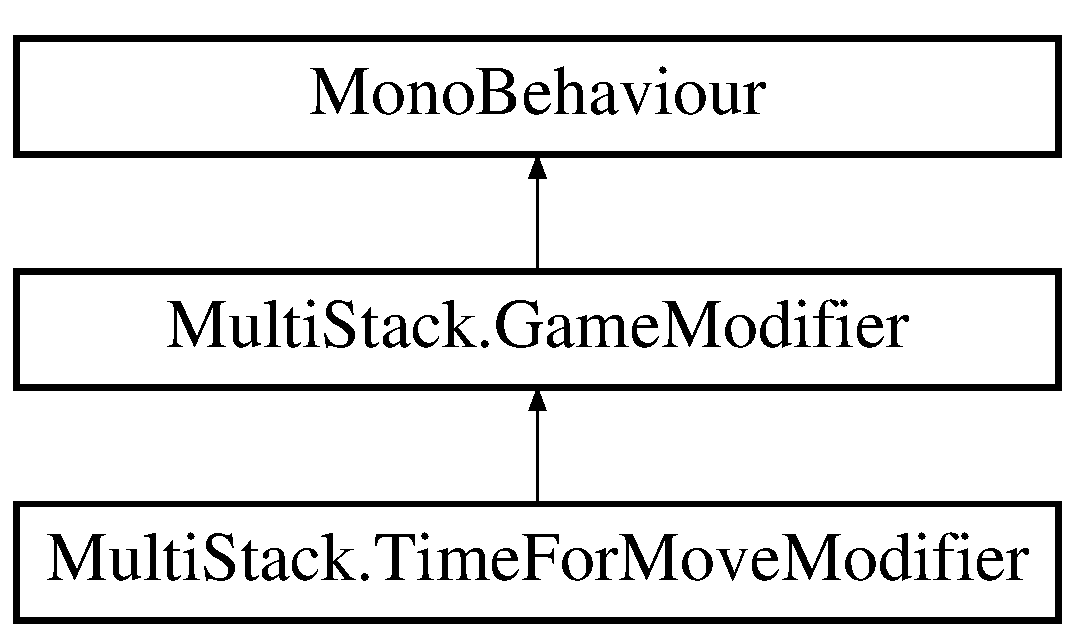
\includegraphics[height=3.000000cm]{class_multi_stack_1_1_time_for_move_modifier}
\end{center}
\end{figure}
\subsection*{Public Member Functions}
\begin{DoxyCompactItemize}
\item 
override void \hyperlink{class_multi_stack_1_1_time_for_move_modifier_a20bbbf8a51e48116235eff90cfa841a3}{Activate} ()
\begin{DoxyCompactList}\small\item\em Activate this modifier. Called at the beginning of the round. \end{DoxyCompactList}\item 
override void \hyperlink{class_multi_stack_1_1_time_for_move_modifier_a52651c8cbe22e57c0e1d5dd3f4d5fafc}{Deactivate} ()
\begin{DoxyCompactList}\small\item\em Deactivate this modifier. Called before a new modifier is enabled. \end{DoxyCompactList}\end{DoxyCompactItemize}
\subsection*{Public Attributes}
\begin{DoxyCompactItemize}
\item 
int \hyperlink{class_multi_stack_1_1_time_for_move_modifier_af70ee289af6f74c5ef18ef495fbc5c03}{changed\+Time} = 15
\begin{DoxyCompactList}\small\item\em The new move time for this round. \end{DoxyCompactList}\end{DoxyCompactItemize}


\subsection{Detailed Description}
When enabled the time a player has to complete their turn is changed to \hyperlink{class_multi_stack_1_1_time_for_move_modifier_af70ee289af6f74c5ef18ef495fbc5c03}{Multi\+Stack.\+Time\+For\+Move\+Modifier.\+changed\+Time}. 



\subsection{Member Function Documentation}
\hypertarget{class_multi_stack_1_1_time_for_move_modifier_a20bbbf8a51e48116235eff90cfa841a3}{}\index{Multi\+Stack\+::\+Time\+For\+Move\+Modifier@{Multi\+Stack\+::\+Time\+For\+Move\+Modifier}!Activate@{Activate}}
\index{Activate@{Activate}!Multi\+Stack\+::\+Time\+For\+Move\+Modifier@{Multi\+Stack\+::\+Time\+For\+Move\+Modifier}}
\subsubsection[{Activate()}]{\setlength{\rightskip}{0pt plus 5cm}override void Multi\+Stack.\+Time\+For\+Move\+Modifier.\+Activate (
\begin{DoxyParamCaption}
{}
\end{DoxyParamCaption}
)\hspace{0.3cm}{\ttfamily [virtual]}}\label{class_multi_stack_1_1_time_for_move_modifier_a20bbbf8a51e48116235eff90cfa841a3}


Activate this modifier. Called at the beginning of the round. 



Implements \hyperlink{class_multi_stack_1_1_game_modifier_a3fb880f9728f8680bf473ac5c7f6832e}{Multi\+Stack.\+Game\+Modifier}.

\hypertarget{class_multi_stack_1_1_time_for_move_modifier_a52651c8cbe22e57c0e1d5dd3f4d5fafc}{}\index{Multi\+Stack\+::\+Time\+For\+Move\+Modifier@{Multi\+Stack\+::\+Time\+For\+Move\+Modifier}!Deactivate@{Deactivate}}
\index{Deactivate@{Deactivate}!Multi\+Stack\+::\+Time\+For\+Move\+Modifier@{Multi\+Stack\+::\+Time\+For\+Move\+Modifier}}
\subsubsection[{Deactivate()}]{\setlength{\rightskip}{0pt plus 5cm}override void Multi\+Stack.\+Time\+For\+Move\+Modifier.\+Deactivate (
\begin{DoxyParamCaption}
{}
\end{DoxyParamCaption}
)\hspace{0.3cm}{\ttfamily [virtual]}}\label{class_multi_stack_1_1_time_for_move_modifier_a52651c8cbe22e57c0e1d5dd3f4d5fafc}


Deactivate this modifier. Called before a new modifier is enabled. 



Implements \hyperlink{class_multi_stack_1_1_game_modifier_abe04db6ab31f5e5063739d8e5a3f7ad1}{Multi\+Stack.\+Game\+Modifier}.



\subsection{Member Data Documentation}
\hypertarget{class_multi_stack_1_1_time_for_move_modifier_af70ee289af6f74c5ef18ef495fbc5c03}{}\index{Multi\+Stack\+::\+Time\+For\+Move\+Modifier@{Multi\+Stack\+::\+Time\+For\+Move\+Modifier}!changed\+Time@{changed\+Time}}
\index{changed\+Time@{changed\+Time}!Multi\+Stack\+::\+Time\+For\+Move\+Modifier@{Multi\+Stack\+::\+Time\+For\+Move\+Modifier}}
\subsubsection[{changed\+Time}]{\setlength{\rightskip}{0pt plus 5cm}int Multi\+Stack.\+Time\+For\+Move\+Modifier.\+changed\+Time = 15}\label{class_multi_stack_1_1_time_for_move_modifier_af70ee289af6f74c5ef18ef495fbc5c03}


The new move time for this round. 



The documentation for this class was generated from the following file\+:\begin{DoxyCompactItemize}
\item 
Multiplayer\+Stacker/\+Scripts/\+Modifiers/Time\+For\+Move\+Modifier.\+cs\end{DoxyCompactItemize}

\hypertarget{class_multi_stack_1_1_turn_manager}{}\section{Multi\+Stack.\+Turn\+Manager Class Reference}
\label{class_multi_stack_1_1_turn_manager}\index{Multi\+Stack.\+Turn\+Manager@{Multi\+Stack.\+Turn\+Manager}}


Handles player turns an spawning of player physics objects objects. Manages and maintains a list of spawned physics objects. Also handles applying certain \hyperlink{class_multi_stack_1_1_game_modifier}{Multi\+Stack.\+Game\+Modifier} e.\+g. when \hyperlink{class_multi_stack_1_1_explosive_shape_modifier}{Multi\+Stack.\+Explosive\+Shape\+Modifier} is applied, this class will loop through the spawned shape list and convert one shape into an explosive shape.  


Inheritance diagram for Multi\+Stack.\+Turn\+Manager\+:\begin{figure}[H]
\begin{center}
\leavevmode
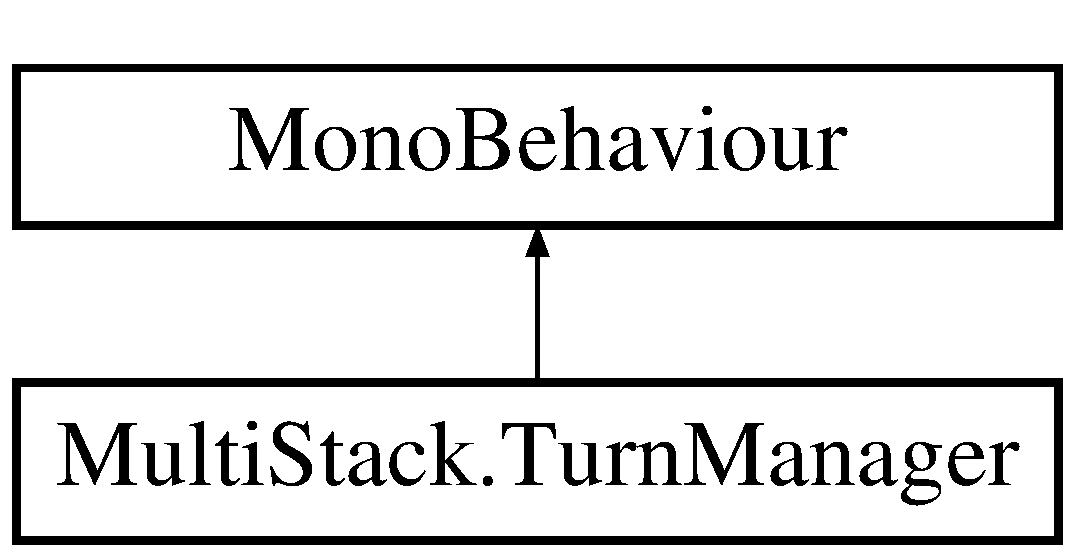
\includegraphics[height=2.000000cm]{class_multi_stack_1_1_turn_manager}
\end{center}
\end{figure}
\subsection*{Public Member Functions}
\begin{DoxyCompactItemize}
\item 
void \hyperlink{class_multi_stack_1_1_turn_manager_ada486b044c24c99626a87dd09c5bd44a}{Initialise} (int num\+Of\+Players)
\begin{DoxyCompactList}\small\item\em Sets number of players. Loads \hyperlink{class_multi_stack_1_1_turn_manager_a4c217abcf3dd22bc5aa3908aa68c0df3}{Multi\+Stack.\+Turn\+Manager.\+physics\+Objects}. \end{DoxyCompactList}\item 
void \hyperlink{class_multi_stack_1_1_turn_manager_a5ecde21a2b9c4d25fa781e717a946700}{Change\+Shape\+To\+Glass} ()
\begin{DoxyCompactList}\small\item\em Changes a shape to glass. The most recent shape that can be turn into glass is selected. \end{DoxyCompactList}\item 
void \hyperlink{class_multi_stack_1_1_turn_manager_a4366a75c5431c6d38c2feeb650f07d54}{Change\+Shape\+To\+Explosive} ()
\begin{DoxyCompactList}\small\item\em Changes a shape to explosive. The most recent shape that can be turned into an explosive is selected. \end{DoxyCompactList}\item 
void \hyperlink{class_multi_stack_1_1_turn_manager_a91108690df912e6108e9fb618df72708}{Object\+Picked\+Up} (Rigidbody2\+D obj)
\begin{DoxyCompactList}\small\item\em Specifies that an object has been picked up. This is used to help decide if the current player has finished their turn. \end{DoxyCompactList}\item 
void \hyperlink{class_multi_stack_1_1_turn_manager_aaca45e591f6687226f10d9a9e385e7f9}{Object\+Dropped} (Rigidbody2\+D obj)
\begin{DoxyCompactList}\small\item\em Specifies that an object has been picked dropped. This is used to help decide if the current player has finished their turn. \end{DoxyCompactList}\item 
void \hyperlink{class_multi_stack_1_1_turn_manager_ae7cb8bf242a4c9cc7285be6aa8d3efb8}{Start\+New\+Round} ()
\begin{DoxyCompactList}\small\item\em Starts a new round, increments current round counter and begins a new turn if not gameover. \end{DoxyCompactList}\item 
void \hyperlink{class_multi_stack_1_1_turn_manager_af375fbee3096867b8337e75b8e4a06de}{Apply\+Gravity\+Modifier} (float modifier)
\begin{DoxyCompactList}\small\item\em Loops through each spawned physics object and multiplies the gravvity scale by the modifier. \end{DoxyCompactList}\item 
void \hyperlink{class_multi_stack_1_1_turn_manager_a4e0f7de949f3cb912cdbe98a195dcd04}{Disable\+Gravity\+Modifier} ()
\begin{DoxyCompactList}\small\item\em Disables the gravity modifier. Resets each spawned physics object gravity scale. \end{DoxyCompactList}\item 
void \hyperlink{class_multi_stack_1_1_turn_manager_aaaf4f4aa21ffbbb776f8aaa779cf132f}{Apply\+Size\+Modifier} (float modifier)
\begin{DoxyCompactList}\small\item\em Applies a size modifier to each spawned physics object for this round. \end{DoxyCompactList}\item 
void \hyperlink{class_multi_stack_1_1_turn_manager_a8755e3ed0f28537cea3ae261ec9521d1}{Disable\+Size\+Modifier} ()
\begin{DoxyCompactList}\small\item\em Disables the size modifier. \end{DoxyCompactList}\item 
void \hyperlink{class_multi_stack_1_1_turn_manager_ad1754c98a2d10824c3a0b17928e49f82}{Apply\+Shape\+Modifier} (\hyperlink{namespace_multi_stack_ac7f637887fea673ceeae6fdd0598c048}{Shape} shape)
\begin{DoxyCompactList}\small\item\em When invoked only the specified shape will be spawned this round. \end{DoxyCompactList}\item 
void \hyperlink{class_multi_stack_1_1_turn_manager_a6e51d749d36ac99a6c83abe227f44160}{Disable\+Shape\+Modifier} ()
\begin{DoxyCompactList}\small\item\em Disables the shape modifier. Any type of shape will be spawned next round. \end{DoxyCompactList}\item 
void \hyperlink{class_multi_stack_1_1_turn_manager_a12f7087435556824abf79e14c8e52204}{Apply\+Catch\+The\+Shape\+Modifier} ()
\begin{DoxyCompactList}\small\item\em Applies the catch the shape modifier. When this is activated, when a shape is spawned it is dropped and the player has to catch it before it falls. \end{DoxyCompactList}\item 
void \hyperlink{class_multi_stack_1_1_turn_manager_a01e22ec6056a36b65ec0d8afd563dd8d}{Disable\+Catch\+The\+Shape\+Modifier} ()
\begin{DoxyCompactList}\small\item\em Disables the catch the shape modifier. \end{DoxyCompactList}\end{DoxyCompactItemize}
\subsection*{Public Attributes}
\begin{DoxyCompactItemize}
\item 
Transform\mbox{[}$\,$\mbox{]} \hyperlink{class_multi_stack_1_1_turn_manager_a4693285de295363939a9f454ac6a5e5b}{player\+Locations}
\begin{DoxyCompactList}\small\item\em The player locations where the plays shape will spawn. \end{DoxyCompactList}\item 
\hyperlink{struct_multi_stack_1_1_player_physics_object}{Player\+Physics\+Object}\mbox{[}$\,$\mbox{]} \hyperlink{class_multi_stack_1_1_turn_manager_a4c217abcf3dd22bc5aa3908aa68c0df3}{physics\+Objects}
\begin{DoxyCompactList}\small\item\em The physics objects that can be spawned. \end{DoxyCompactList}\item 
\hyperlink{class_multi_stack_1_1_game_text}{Game\+Text} \hyperlink{class_multi_stack_1_1_turn_manager_a498a14eba4b58bc373456efba57302fa}{player\+Text}
\begin{DoxyCompactList}\small\item\em The U\+I that will inform the player it is their turn. \end{DoxyCompactList}\item 
\hyperlink{class_multi_stack_1_1_game_text}{Game\+Text} \hyperlink{class_multi_stack_1_1_turn_manager_a2084e64bcf723c4d9d46960f18c26368}{time\+Remaining\+Text}
\begin{DoxyCompactList}\small\item\em The U\+I that shows the current players time remaining for their turn. \end{DoxyCompactList}\item 
\hyperlink{class_multi_stack_1_1_player_colours}{Player\+Colours} \hyperlink{class_multi_stack_1_1_turn_manager_a21fba5ca2fc616a5f1dde0676ba9f5f2}{player\+Colours}
\begin{DoxyCompactList}\small\item\em The player colours. The \hyperlink{class_multi_stack_1_1_turn_manager_a498a14eba4b58bc373456efba57302fa}{Multi\+Stack.\+Turn\+Manager.\+player\+Text} U\+I is shown in the current players colour. \end{DoxyCompactList}\item 
int \hyperlink{class_multi_stack_1_1_turn_manager_aac198a78f07eea0eae4e12fe100ea043}{base\+Time\+For\+Move} = 20
\begin{DoxyCompactList}\small\item\em The base tim (without modifiers) that each player has to complete their turn. \end{DoxyCompactList}\end{DoxyCompactItemize}
\subsection*{Properties}
\begin{DoxyCompactItemize}
\item 
int \hyperlink{class_multi_stack_1_1_turn_manager_a74740c372c337673c08f6fe42cd35f5a}{current\+Round}\hspace{0.3cm}{\ttfamily  \mbox{[}get\mbox{]}}
\begin{DoxyCompactList}\small\item\em The current round number. \end{DoxyCompactList}\item 
int \hyperlink{class_multi_stack_1_1_turn_manager_a02c135523dbabc3d7eef1467e567ec7c}{current\+Enhanced\+Height}\hspace{0.3cm}{\ttfamily  \mbox{[}get\mbox{]}}
\begin{DoxyCompactList}\small\item\em Gets the height of the current stack of physics objects + 4f. This is used for the U\+I. \end{DoxyCompactList}\item 
float \hyperlink{class_multi_stack_1_1_turn_manager_a951b024c556f17abe670f53ba30089f1}{shape\+Offset\+Height}\hspace{0.3cm}{\ttfamily  \mbox{[}get\mbox{]}}
\begin{DoxyCompactList}\small\item\em Gets the height of the shape stack offset. Used by the \hyperlink{class_multi_stack_1_1_camera_manager}{Multi\+Stack.\+Camera\+Manager} to limit how far the camera can scroll upwards. \end{DoxyCompactList}\item 
int \hyperlink{class_multi_stack_1_1_turn_manager_a386f4ecd851d1c9ef639ceaf7d31e439}{num\+Of\+Objects\+Spawned}\hspace{0.3cm}{\ttfamily  \mbox{[}get\mbox{]}}
\begin{DoxyCompactList}\small\item\em The number of physics objects in the current scene. \end{DoxyCompactList}\item 
bool \hyperlink{class_multi_stack_1_1_turn_manager_aa811a8a5c996e0cf99295d7829727874}{explosive\+Sprite\+Available\+For\+Spawned\+Object}\hspace{0.3cm}{\ttfamily  \mbox{[}get\mbox{]}}
\begin{DoxyCompactList}\small\item\em Gets a value indicating whether this \hyperlink{class_multi_stack_1_1_turn_manager}{Multi\+Stack.\+Turn\+Manager} has spawned a physics object that can be turned into an explosive object. \end{DoxyCompactList}\item 
bool \hyperlink{class_multi_stack_1_1_turn_manager_a2e2e26f02fda080730d6bd6c5e837e72}{glass\+Sprite\+Available\+For\+Spawned\+Object}\hspace{0.3cm}{\ttfamily  \mbox{[}get\mbox{]}}
\begin{DoxyCompactList}\small\item\em Gets a value indicating whether this \hyperlink{class_multi_stack_1_1_turn_manager}{Multi\+Stack.\+Turn\+Manager} has spawned an object that can be turned into a glass object. \end{DoxyCompactList}\item 
bool \hyperlink{class_multi_stack_1_1_turn_manager_afbc6bb1a22b590b63ec2b7b496598352}{random\+Player\+Order}\hspace{0.3cm}{\ttfamily  \mbox{[}set\mbox{]}}
\begin{DoxyCompactList}\small\item\em Sets a value indicating whether this \hyperlink{class_multi_stack_1_1_turn_manager}{Multi\+Stack.\+Turn\+Manager} should shuffle the players for the next round. \end{DoxyCompactList}\item 
int \hyperlink{class_multi_stack_1_1_turn_manager_a308c362d6c9ad9c8ca5f2e039ca76f90}{current\+Player}\hspace{0.3cm}{\ttfamily  \mbox{[}get\mbox{]}}
\begin{DoxyCompactList}\small\item\em The index of the current player. \end{DoxyCompactList}\item 
bool \hyperlink{class_multi_stack_1_1_turn_manager_a623b9a24f294fbbaa819e9149f9f0135}{should\+Update}\hspace{0.3cm}{\ttfamily  \mbox{[}set\mbox{]}}
\begin{DoxyCompactList}\small\item\em Sets a value indicating whether this \hyperlink{class_multi_stack_1_1_turn_manager}{Multi\+Stack.\+Turn\+Manager} should update. \end{DoxyCompactList}\item 
static \hyperlink{class_multi_stack_1_1_turn_manager}{Turn\+Manager} \hyperlink{class_multi_stack_1_1_turn_manager_a7da3b19311001850c30860447304a5b4}{instance}\hspace{0.3cm}{\ttfamily  \mbox{[}get\mbox{]}}
\begin{DoxyCompactList}\small\item\em Signleton pattern. Gets the instance. Accessible from any class. \end{DoxyCompactList}\end{DoxyCompactItemize}


\subsection{Detailed Description}
Handles player turns an spawning of player physics objects objects. Manages and maintains a list of spawned physics objects. Also handles applying certain \hyperlink{class_multi_stack_1_1_game_modifier}{Multi\+Stack.\+Game\+Modifier} e.\+g. when \hyperlink{class_multi_stack_1_1_explosive_shape_modifier}{Multi\+Stack.\+Explosive\+Shape\+Modifier} is applied, this class will loop through the spawned shape list and convert one shape into an explosive shape. 



\subsection{Member Function Documentation}
\hypertarget{class_multi_stack_1_1_turn_manager_a12f7087435556824abf79e14c8e52204}{}\index{Multi\+Stack\+::\+Turn\+Manager@{Multi\+Stack\+::\+Turn\+Manager}!Apply\+Catch\+The\+Shape\+Modifier@{Apply\+Catch\+The\+Shape\+Modifier}}
\index{Apply\+Catch\+The\+Shape\+Modifier@{Apply\+Catch\+The\+Shape\+Modifier}!Multi\+Stack\+::\+Turn\+Manager@{Multi\+Stack\+::\+Turn\+Manager}}
\subsubsection[{Apply\+Catch\+The\+Shape\+Modifier()}]{\setlength{\rightskip}{0pt plus 5cm}void Multi\+Stack.\+Turn\+Manager.\+Apply\+Catch\+The\+Shape\+Modifier (
\begin{DoxyParamCaption}
{}
\end{DoxyParamCaption}
)}\label{class_multi_stack_1_1_turn_manager_a12f7087435556824abf79e14c8e52204}


Applies the catch the shape modifier. When this is activated, when a shape is spawned it is dropped and the player has to catch it before it falls. 

\hypertarget{class_multi_stack_1_1_turn_manager_af375fbee3096867b8337e75b8e4a06de}{}\index{Multi\+Stack\+::\+Turn\+Manager@{Multi\+Stack\+::\+Turn\+Manager}!Apply\+Gravity\+Modifier@{Apply\+Gravity\+Modifier}}
\index{Apply\+Gravity\+Modifier@{Apply\+Gravity\+Modifier}!Multi\+Stack\+::\+Turn\+Manager@{Multi\+Stack\+::\+Turn\+Manager}}
\subsubsection[{Apply\+Gravity\+Modifier(float modifier)}]{\setlength{\rightskip}{0pt plus 5cm}void Multi\+Stack.\+Turn\+Manager.\+Apply\+Gravity\+Modifier (
\begin{DoxyParamCaption}
\item[{float}]{modifier}
\end{DoxyParamCaption}
)}\label{class_multi_stack_1_1_turn_manager_af375fbee3096867b8337e75b8e4a06de}


Loops through each spawned physics object and multiplies the gravvity scale by the modifier. 


\begin{DoxyParams}{Parameters}
{\em modifier} & Modifier.\\
\hline
\end{DoxyParams}
\hypertarget{class_multi_stack_1_1_turn_manager_ad1754c98a2d10824c3a0b17928e49f82}{}\index{Multi\+Stack\+::\+Turn\+Manager@{Multi\+Stack\+::\+Turn\+Manager}!Apply\+Shape\+Modifier@{Apply\+Shape\+Modifier}}
\index{Apply\+Shape\+Modifier@{Apply\+Shape\+Modifier}!Multi\+Stack\+::\+Turn\+Manager@{Multi\+Stack\+::\+Turn\+Manager}}
\subsubsection[{Apply\+Shape\+Modifier(\+Shape shape)}]{\setlength{\rightskip}{0pt plus 5cm}void Multi\+Stack.\+Turn\+Manager.\+Apply\+Shape\+Modifier (
\begin{DoxyParamCaption}
\item[{{\bf Shape}}]{shape}
\end{DoxyParamCaption}
)}\label{class_multi_stack_1_1_turn_manager_ad1754c98a2d10824c3a0b17928e49f82}


When invoked only the specified shape will be spawned this round. 


\begin{DoxyParams}{Parameters}
{\em shape} & Shape.\\
\hline
\end{DoxyParams}
\hypertarget{class_multi_stack_1_1_turn_manager_aaaf4f4aa21ffbbb776f8aaa779cf132f}{}\index{Multi\+Stack\+::\+Turn\+Manager@{Multi\+Stack\+::\+Turn\+Manager}!Apply\+Size\+Modifier@{Apply\+Size\+Modifier}}
\index{Apply\+Size\+Modifier@{Apply\+Size\+Modifier}!Multi\+Stack\+::\+Turn\+Manager@{Multi\+Stack\+::\+Turn\+Manager}}
\subsubsection[{Apply\+Size\+Modifier(float modifier)}]{\setlength{\rightskip}{0pt plus 5cm}void Multi\+Stack.\+Turn\+Manager.\+Apply\+Size\+Modifier (
\begin{DoxyParamCaption}
\item[{float}]{modifier}
\end{DoxyParamCaption}
)}\label{class_multi_stack_1_1_turn_manager_aaaf4f4aa21ffbbb776f8aaa779cf132f}


Applies a size modifier to each spawned physics object for this round. 


\begin{DoxyParams}{Parameters}
{\em modifier} & Modifier.\\
\hline
\end{DoxyParams}
\hypertarget{class_multi_stack_1_1_turn_manager_a4366a75c5431c6d38c2feeb650f07d54}{}\index{Multi\+Stack\+::\+Turn\+Manager@{Multi\+Stack\+::\+Turn\+Manager}!Change\+Shape\+To\+Explosive@{Change\+Shape\+To\+Explosive}}
\index{Change\+Shape\+To\+Explosive@{Change\+Shape\+To\+Explosive}!Multi\+Stack\+::\+Turn\+Manager@{Multi\+Stack\+::\+Turn\+Manager}}
\subsubsection[{Change\+Shape\+To\+Explosive()}]{\setlength{\rightskip}{0pt plus 5cm}void Multi\+Stack.\+Turn\+Manager.\+Change\+Shape\+To\+Explosive (
\begin{DoxyParamCaption}
{}
\end{DoxyParamCaption}
)}\label{class_multi_stack_1_1_turn_manager_a4366a75c5431c6d38c2feeb650f07d54}


Changes a shape to explosive. The most recent shape that can be turned into an explosive is selected. 

\hypertarget{class_multi_stack_1_1_turn_manager_a5ecde21a2b9c4d25fa781e717a946700}{}\index{Multi\+Stack\+::\+Turn\+Manager@{Multi\+Stack\+::\+Turn\+Manager}!Change\+Shape\+To\+Glass@{Change\+Shape\+To\+Glass}}
\index{Change\+Shape\+To\+Glass@{Change\+Shape\+To\+Glass}!Multi\+Stack\+::\+Turn\+Manager@{Multi\+Stack\+::\+Turn\+Manager}}
\subsubsection[{Change\+Shape\+To\+Glass()}]{\setlength{\rightskip}{0pt plus 5cm}void Multi\+Stack.\+Turn\+Manager.\+Change\+Shape\+To\+Glass (
\begin{DoxyParamCaption}
{}
\end{DoxyParamCaption}
)}\label{class_multi_stack_1_1_turn_manager_a5ecde21a2b9c4d25fa781e717a946700}


Changes a shape to glass. The most recent shape that can be turn into glass is selected. 

\hypertarget{class_multi_stack_1_1_turn_manager_a01e22ec6056a36b65ec0d8afd563dd8d}{}\index{Multi\+Stack\+::\+Turn\+Manager@{Multi\+Stack\+::\+Turn\+Manager}!Disable\+Catch\+The\+Shape\+Modifier@{Disable\+Catch\+The\+Shape\+Modifier}}
\index{Disable\+Catch\+The\+Shape\+Modifier@{Disable\+Catch\+The\+Shape\+Modifier}!Multi\+Stack\+::\+Turn\+Manager@{Multi\+Stack\+::\+Turn\+Manager}}
\subsubsection[{Disable\+Catch\+The\+Shape\+Modifier()}]{\setlength{\rightskip}{0pt plus 5cm}void Multi\+Stack.\+Turn\+Manager.\+Disable\+Catch\+The\+Shape\+Modifier (
\begin{DoxyParamCaption}
{}
\end{DoxyParamCaption}
)}\label{class_multi_stack_1_1_turn_manager_a01e22ec6056a36b65ec0d8afd563dd8d}


Disables the catch the shape modifier. 

\hypertarget{class_multi_stack_1_1_turn_manager_a4e0f7de949f3cb912cdbe98a195dcd04}{}\index{Multi\+Stack\+::\+Turn\+Manager@{Multi\+Stack\+::\+Turn\+Manager}!Disable\+Gravity\+Modifier@{Disable\+Gravity\+Modifier}}
\index{Disable\+Gravity\+Modifier@{Disable\+Gravity\+Modifier}!Multi\+Stack\+::\+Turn\+Manager@{Multi\+Stack\+::\+Turn\+Manager}}
\subsubsection[{Disable\+Gravity\+Modifier()}]{\setlength{\rightskip}{0pt plus 5cm}void Multi\+Stack.\+Turn\+Manager.\+Disable\+Gravity\+Modifier (
\begin{DoxyParamCaption}
{}
\end{DoxyParamCaption}
)}\label{class_multi_stack_1_1_turn_manager_a4e0f7de949f3cb912cdbe98a195dcd04}


Disables the gravity modifier. Resets each spawned physics object gravity scale. 

\hypertarget{class_multi_stack_1_1_turn_manager_a6e51d749d36ac99a6c83abe227f44160}{}\index{Multi\+Stack\+::\+Turn\+Manager@{Multi\+Stack\+::\+Turn\+Manager}!Disable\+Shape\+Modifier@{Disable\+Shape\+Modifier}}
\index{Disable\+Shape\+Modifier@{Disable\+Shape\+Modifier}!Multi\+Stack\+::\+Turn\+Manager@{Multi\+Stack\+::\+Turn\+Manager}}
\subsubsection[{Disable\+Shape\+Modifier()}]{\setlength{\rightskip}{0pt plus 5cm}void Multi\+Stack.\+Turn\+Manager.\+Disable\+Shape\+Modifier (
\begin{DoxyParamCaption}
{}
\end{DoxyParamCaption}
)}\label{class_multi_stack_1_1_turn_manager_a6e51d749d36ac99a6c83abe227f44160}


Disables the shape modifier. Any type of shape will be spawned next round. 

\hypertarget{class_multi_stack_1_1_turn_manager_a8755e3ed0f28537cea3ae261ec9521d1}{}\index{Multi\+Stack\+::\+Turn\+Manager@{Multi\+Stack\+::\+Turn\+Manager}!Disable\+Size\+Modifier@{Disable\+Size\+Modifier}}
\index{Disable\+Size\+Modifier@{Disable\+Size\+Modifier}!Multi\+Stack\+::\+Turn\+Manager@{Multi\+Stack\+::\+Turn\+Manager}}
\subsubsection[{Disable\+Size\+Modifier()}]{\setlength{\rightskip}{0pt plus 5cm}void Multi\+Stack.\+Turn\+Manager.\+Disable\+Size\+Modifier (
\begin{DoxyParamCaption}
{}
\end{DoxyParamCaption}
)}\label{class_multi_stack_1_1_turn_manager_a8755e3ed0f28537cea3ae261ec9521d1}


Disables the size modifier. 

\hypertarget{class_multi_stack_1_1_turn_manager_ada486b044c24c99626a87dd09c5bd44a}{}\index{Multi\+Stack\+::\+Turn\+Manager@{Multi\+Stack\+::\+Turn\+Manager}!Initialise@{Initialise}}
\index{Initialise@{Initialise}!Multi\+Stack\+::\+Turn\+Manager@{Multi\+Stack\+::\+Turn\+Manager}}
\subsubsection[{Initialise(int num\+Of\+Players)}]{\setlength{\rightskip}{0pt plus 5cm}void Multi\+Stack.\+Turn\+Manager.\+Initialise (
\begin{DoxyParamCaption}
\item[{int}]{num\+Of\+Players}
\end{DoxyParamCaption}
)}\label{class_multi_stack_1_1_turn_manager_ada486b044c24c99626a87dd09c5bd44a}


Sets number of players. Loads \hyperlink{class_multi_stack_1_1_turn_manager_a4c217abcf3dd22bc5aa3908aa68c0df3}{Multi\+Stack.\+Turn\+Manager.\+physics\+Objects}. 


\begin{DoxyParams}{Parameters}
{\em num\+Of\+Players} & Number of players.\\
\hline
\end{DoxyParams}
\hypertarget{class_multi_stack_1_1_turn_manager_aaca45e591f6687226f10d9a9e385e7f9}{}\index{Multi\+Stack\+::\+Turn\+Manager@{Multi\+Stack\+::\+Turn\+Manager}!Object\+Dropped@{Object\+Dropped}}
\index{Object\+Dropped@{Object\+Dropped}!Multi\+Stack\+::\+Turn\+Manager@{Multi\+Stack\+::\+Turn\+Manager}}
\subsubsection[{Object\+Dropped(\+Rigidbody2\+D obj)}]{\setlength{\rightskip}{0pt plus 5cm}void Multi\+Stack.\+Turn\+Manager.\+Object\+Dropped (
\begin{DoxyParamCaption}
\item[{Rigidbody2\+D}]{obj}
\end{DoxyParamCaption}
)}\label{class_multi_stack_1_1_turn_manager_aaca45e591f6687226f10d9a9e385e7f9}


Specifies that an object has been picked dropped. This is used to help decide if the current player has finished their turn. 


\begin{DoxyParams}{Parameters}
{\em obj} & Object.\\
\hline
\end{DoxyParams}
\hypertarget{class_multi_stack_1_1_turn_manager_a91108690df912e6108e9fb618df72708}{}\index{Multi\+Stack\+::\+Turn\+Manager@{Multi\+Stack\+::\+Turn\+Manager}!Object\+Picked\+Up@{Object\+Picked\+Up}}
\index{Object\+Picked\+Up@{Object\+Picked\+Up}!Multi\+Stack\+::\+Turn\+Manager@{Multi\+Stack\+::\+Turn\+Manager}}
\subsubsection[{Object\+Picked\+Up(\+Rigidbody2\+D obj)}]{\setlength{\rightskip}{0pt plus 5cm}void Multi\+Stack.\+Turn\+Manager.\+Object\+Picked\+Up (
\begin{DoxyParamCaption}
\item[{Rigidbody2\+D}]{obj}
\end{DoxyParamCaption}
)}\label{class_multi_stack_1_1_turn_manager_a91108690df912e6108e9fb618df72708}


Specifies that an object has been picked up. This is used to help decide if the current player has finished their turn. 


\begin{DoxyParams}{Parameters}
{\em obj} & Object.\\
\hline
\end{DoxyParams}
\hypertarget{class_multi_stack_1_1_turn_manager_ae7cb8bf242a4c9cc7285be6aa8d3efb8}{}\index{Multi\+Stack\+::\+Turn\+Manager@{Multi\+Stack\+::\+Turn\+Manager}!Start\+New\+Round@{Start\+New\+Round}}
\index{Start\+New\+Round@{Start\+New\+Round}!Multi\+Stack\+::\+Turn\+Manager@{Multi\+Stack\+::\+Turn\+Manager}}
\subsubsection[{Start\+New\+Round()}]{\setlength{\rightskip}{0pt plus 5cm}void Multi\+Stack.\+Turn\+Manager.\+Start\+New\+Round (
\begin{DoxyParamCaption}
{}
\end{DoxyParamCaption}
)}\label{class_multi_stack_1_1_turn_manager_ae7cb8bf242a4c9cc7285be6aa8d3efb8}


Starts a new round, increments current round counter and begins a new turn if not gameover. 



\subsection{Member Data Documentation}
\hypertarget{class_multi_stack_1_1_turn_manager_aac198a78f07eea0eae4e12fe100ea043}{}\index{Multi\+Stack\+::\+Turn\+Manager@{Multi\+Stack\+::\+Turn\+Manager}!base\+Time\+For\+Move@{base\+Time\+For\+Move}}
\index{base\+Time\+For\+Move@{base\+Time\+For\+Move}!Multi\+Stack\+::\+Turn\+Manager@{Multi\+Stack\+::\+Turn\+Manager}}
\subsubsection[{base\+Time\+For\+Move}]{\setlength{\rightskip}{0pt plus 5cm}int Multi\+Stack.\+Turn\+Manager.\+base\+Time\+For\+Move = 20}\label{class_multi_stack_1_1_turn_manager_aac198a78f07eea0eae4e12fe100ea043}


The base tim (without modifiers) that each player has to complete their turn. 

\hypertarget{class_multi_stack_1_1_turn_manager_a4c217abcf3dd22bc5aa3908aa68c0df3}{}\index{Multi\+Stack\+::\+Turn\+Manager@{Multi\+Stack\+::\+Turn\+Manager}!physics\+Objects@{physics\+Objects}}
\index{physics\+Objects@{physics\+Objects}!Multi\+Stack\+::\+Turn\+Manager@{Multi\+Stack\+::\+Turn\+Manager}}
\subsubsection[{physics\+Objects}]{\setlength{\rightskip}{0pt plus 5cm}{\bf Player\+Physics\+Object} \mbox{[}$\,$\mbox{]} Multi\+Stack.\+Turn\+Manager.\+physics\+Objects}\label{class_multi_stack_1_1_turn_manager_a4c217abcf3dd22bc5aa3908aa68c0df3}


The physics objects that can be spawned. 

\hypertarget{class_multi_stack_1_1_turn_manager_a21fba5ca2fc616a5f1dde0676ba9f5f2}{}\index{Multi\+Stack\+::\+Turn\+Manager@{Multi\+Stack\+::\+Turn\+Manager}!player\+Colours@{player\+Colours}}
\index{player\+Colours@{player\+Colours}!Multi\+Stack\+::\+Turn\+Manager@{Multi\+Stack\+::\+Turn\+Manager}}
\subsubsection[{player\+Colours}]{\setlength{\rightskip}{0pt plus 5cm}{\bf Player\+Colours} Multi\+Stack.\+Turn\+Manager.\+player\+Colours}\label{class_multi_stack_1_1_turn_manager_a21fba5ca2fc616a5f1dde0676ba9f5f2}


The player colours. The \hyperlink{class_multi_stack_1_1_turn_manager_a498a14eba4b58bc373456efba57302fa}{Multi\+Stack.\+Turn\+Manager.\+player\+Text} U\+I is shown in the current players colour. 

\hypertarget{class_multi_stack_1_1_turn_manager_a4693285de295363939a9f454ac6a5e5b}{}\index{Multi\+Stack\+::\+Turn\+Manager@{Multi\+Stack\+::\+Turn\+Manager}!player\+Locations@{player\+Locations}}
\index{player\+Locations@{player\+Locations}!Multi\+Stack\+::\+Turn\+Manager@{Multi\+Stack\+::\+Turn\+Manager}}
\subsubsection[{player\+Locations}]{\setlength{\rightskip}{0pt plus 5cm}Transform \mbox{[}$\,$\mbox{]} Multi\+Stack.\+Turn\+Manager.\+player\+Locations}\label{class_multi_stack_1_1_turn_manager_a4693285de295363939a9f454ac6a5e5b}


The player locations where the plays shape will spawn. 

\hypertarget{class_multi_stack_1_1_turn_manager_a498a14eba4b58bc373456efba57302fa}{}\index{Multi\+Stack\+::\+Turn\+Manager@{Multi\+Stack\+::\+Turn\+Manager}!player\+Text@{player\+Text}}
\index{player\+Text@{player\+Text}!Multi\+Stack\+::\+Turn\+Manager@{Multi\+Stack\+::\+Turn\+Manager}}
\subsubsection[{player\+Text}]{\setlength{\rightskip}{0pt plus 5cm}{\bf Game\+Text} Multi\+Stack.\+Turn\+Manager.\+player\+Text}\label{class_multi_stack_1_1_turn_manager_a498a14eba4b58bc373456efba57302fa}


The U\+I that will inform the player it is their turn. 

\hypertarget{class_multi_stack_1_1_turn_manager_a2084e64bcf723c4d9d46960f18c26368}{}\index{Multi\+Stack\+::\+Turn\+Manager@{Multi\+Stack\+::\+Turn\+Manager}!time\+Remaining\+Text@{time\+Remaining\+Text}}
\index{time\+Remaining\+Text@{time\+Remaining\+Text}!Multi\+Stack\+::\+Turn\+Manager@{Multi\+Stack\+::\+Turn\+Manager}}
\subsubsection[{time\+Remaining\+Text}]{\setlength{\rightskip}{0pt plus 5cm}{\bf Game\+Text} Multi\+Stack.\+Turn\+Manager.\+time\+Remaining\+Text}\label{class_multi_stack_1_1_turn_manager_a2084e64bcf723c4d9d46960f18c26368}


The U\+I that shows the current players time remaining for their turn. 



\subsection{Property Documentation}
\hypertarget{class_multi_stack_1_1_turn_manager_a02c135523dbabc3d7eef1467e567ec7c}{}\index{Multi\+Stack\+::\+Turn\+Manager@{Multi\+Stack\+::\+Turn\+Manager}!current\+Enhanced\+Height@{current\+Enhanced\+Height}}
\index{current\+Enhanced\+Height@{current\+Enhanced\+Height}!Multi\+Stack\+::\+Turn\+Manager@{Multi\+Stack\+::\+Turn\+Manager}}
\subsubsection[{current\+Enhanced\+Height}]{\setlength{\rightskip}{0pt plus 5cm}int Multi\+Stack.\+Turn\+Manager.\+current\+Enhanced\+Height\hspace{0.3cm}{\ttfamily [get]}}\label{class_multi_stack_1_1_turn_manager_a02c135523dbabc3d7eef1467e567ec7c}


Gets the height of the current stack of physics objects + 4f. This is used for the U\+I. 

The height of the current.\hypertarget{class_multi_stack_1_1_turn_manager_a308c362d6c9ad9c8ca5f2e039ca76f90}{}\index{Multi\+Stack\+::\+Turn\+Manager@{Multi\+Stack\+::\+Turn\+Manager}!current\+Player@{current\+Player}}
\index{current\+Player@{current\+Player}!Multi\+Stack\+::\+Turn\+Manager@{Multi\+Stack\+::\+Turn\+Manager}}
\subsubsection[{current\+Player}]{\setlength{\rightskip}{0pt plus 5cm}int Multi\+Stack.\+Turn\+Manager.\+current\+Player\hspace{0.3cm}{\ttfamily [get]}}\label{class_multi_stack_1_1_turn_manager_a308c362d6c9ad9c8ca5f2e039ca76f90}


The index of the current player. 

The current player.\hypertarget{class_multi_stack_1_1_turn_manager_a74740c372c337673c08f6fe42cd35f5a}{}\index{Multi\+Stack\+::\+Turn\+Manager@{Multi\+Stack\+::\+Turn\+Manager}!current\+Round@{current\+Round}}
\index{current\+Round@{current\+Round}!Multi\+Stack\+::\+Turn\+Manager@{Multi\+Stack\+::\+Turn\+Manager}}
\subsubsection[{current\+Round}]{\setlength{\rightskip}{0pt plus 5cm}int Multi\+Stack.\+Turn\+Manager.\+current\+Round\hspace{0.3cm}{\ttfamily [get]}}\label{class_multi_stack_1_1_turn_manager_a74740c372c337673c08f6fe42cd35f5a}


The current round number. 

The current round.\hypertarget{class_multi_stack_1_1_turn_manager_aa811a8a5c996e0cf99295d7829727874}{}\index{Multi\+Stack\+::\+Turn\+Manager@{Multi\+Stack\+::\+Turn\+Manager}!explosive\+Sprite\+Available\+For\+Spawned\+Object@{explosive\+Sprite\+Available\+For\+Spawned\+Object}}
\index{explosive\+Sprite\+Available\+For\+Spawned\+Object@{explosive\+Sprite\+Available\+For\+Spawned\+Object}!Multi\+Stack\+::\+Turn\+Manager@{Multi\+Stack\+::\+Turn\+Manager}}
\subsubsection[{explosive\+Sprite\+Available\+For\+Spawned\+Object}]{\setlength{\rightskip}{0pt plus 5cm}bool Multi\+Stack.\+Turn\+Manager.\+explosive\+Sprite\+Available\+For\+Spawned\+Object\hspace{0.3cm}{\ttfamily [get]}}\label{class_multi_stack_1_1_turn_manager_aa811a8a5c996e0cf99295d7829727874}


Gets a value indicating whether this \hyperlink{class_multi_stack_1_1_turn_manager}{Multi\+Stack.\+Turn\+Manager} has spawned a physics object that can be turned into an explosive object. 

{\ttfamily true} if explosive sprite available for spawned object; otherwise, {\ttfamily false}.\hypertarget{class_multi_stack_1_1_turn_manager_a2e2e26f02fda080730d6bd6c5e837e72}{}\index{Multi\+Stack\+::\+Turn\+Manager@{Multi\+Stack\+::\+Turn\+Manager}!glass\+Sprite\+Available\+For\+Spawned\+Object@{glass\+Sprite\+Available\+For\+Spawned\+Object}}
\index{glass\+Sprite\+Available\+For\+Spawned\+Object@{glass\+Sprite\+Available\+For\+Spawned\+Object}!Multi\+Stack\+::\+Turn\+Manager@{Multi\+Stack\+::\+Turn\+Manager}}
\subsubsection[{glass\+Sprite\+Available\+For\+Spawned\+Object}]{\setlength{\rightskip}{0pt plus 5cm}bool Multi\+Stack.\+Turn\+Manager.\+glass\+Sprite\+Available\+For\+Spawned\+Object\hspace{0.3cm}{\ttfamily [get]}}\label{class_multi_stack_1_1_turn_manager_a2e2e26f02fda080730d6bd6c5e837e72}


Gets a value indicating whether this \hyperlink{class_multi_stack_1_1_turn_manager}{Multi\+Stack.\+Turn\+Manager} has spawned an object that can be turned into a glass object. 

{\ttfamily true} if glass sprite available for spawned object; otherwise, {\ttfamily false}.\hypertarget{class_multi_stack_1_1_turn_manager_a7da3b19311001850c30860447304a5b4}{}\index{Multi\+Stack\+::\+Turn\+Manager@{Multi\+Stack\+::\+Turn\+Manager}!instance@{instance}}
\index{instance@{instance}!Multi\+Stack\+::\+Turn\+Manager@{Multi\+Stack\+::\+Turn\+Manager}}
\subsubsection[{instance}]{\setlength{\rightskip}{0pt plus 5cm}{\bf Turn\+Manager} Multi\+Stack.\+Turn\+Manager.\+instance\hspace{0.3cm}{\ttfamily [static]}, {\ttfamily [get]}}\label{class_multi_stack_1_1_turn_manager_a7da3b19311001850c30860447304a5b4}


Signleton pattern. Gets the instance. Accessible from any class. 

The instance.\hypertarget{class_multi_stack_1_1_turn_manager_a386f4ecd851d1c9ef639ceaf7d31e439}{}\index{Multi\+Stack\+::\+Turn\+Manager@{Multi\+Stack\+::\+Turn\+Manager}!num\+Of\+Objects\+Spawned@{num\+Of\+Objects\+Spawned}}
\index{num\+Of\+Objects\+Spawned@{num\+Of\+Objects\+Spawned}!Multi\+Stack\+::\+Turn\+Manager@{Multi\+Stack\+::\+Turn\+Manager}}
\subsubsection[{num\+Of\+Objects\+Spawned}]{\setlength{\rightskip}{0pt plus 5cm}int Multi\+Stack.\+Turn\+Manager.\+num\+Of\+Objects\+Spawned\hspace{0.3cm}{\ttfamily [get]}}\label{class_multi_stack_1_1_turn_manager_a386f4ecd851d1c9ef639ceaf7d31e439}


The number of physics objects in the current scene. 

The number of objects spawned.\hypertarget{class_multi_stack_1_1_turn_manager_afbc6bb1a22b590b63ec2b7b496598352}{}\index{Multi\+Stack\+::\+Turn\+Manager@{Multi\+Stack\+::\+Turn\+Manager}!random\+Player\+Order@{random\+Player\+Order}}
\index{random\+Player\+Order@{random\+Player\+Order}!Multi\+Stack\+::\+Turn\+Manager@{Multi\+Stack\+::\+Turn\+Manager}}
\subsubsection[{random\+Player\+Order}]{\setlength{\rightskip}{0pt plus 5cm}bool Multi\+Stack.\+Turn\+Manager.\+random\+Player\+Order\hspace{0.3cm}{\ttfamily [set]}}\label{class_multi_stack_1_1_turn_manager_afbc6bb1a22b590b63ec2b7b496598352}


Sets a value indicating whether this \hyperlink{class_multi_stack_1_1_turn_manager}{Multi\+Stack.\+Turn\+Manager} should shuffle the players for the next round. 

{\ttfamily true} if random player order; otherwise, {\ttfamily false}.\hypertarget{class_multi_stack_1_1_turn_manager_a951b024c556f17abe670f53ba30089f1}{}\index{Multi\+Stack\+::\+Turn\+Manager@{Multi\+Stack\+::\+Turn\+Manager}!shape\+Offset\+Height@{shape\+Offset\+Height}}
\index{shape\+Offset\+Height@{shape\+Offset\+Height}!Multi\+Stack\+::\+Turn\+Manager@{Multi\+Stack\+::\+Turn\+Manager}}
\subsubsection[{shape\+Offset\+Height}]{\setlength{\rightskip}{0pt plus 5cm}float Multi\+Stack.\+Turn\+Manager.\+shape\+Offset\+Height\hspace{0.3cm}{\ttfamily [get]}}\label{class_multi_stack_1_1_turn_manager_a951b024c556f17abe670f53ba30089f1}


Gets the height of the shape stack offset. Used by the \hyperlink{class_multi_stack_1_1_camera_manager}{Multi\+Stack.\+Camera\+Manager} to limit how far the camera can scroll upwards. 

The height of the shape offset.\hypertarget{class_multi_stack_1_1_turn_manager_a623b9a24f294fbbaa819e9149f9f0135}{}\index{Multi\+Stack\+::\+Turn\+Manager@{Multi\+Stack\+::\+Turn\+Manager}!should\+Update@{should\+Update}}
\index{should\+Update@{should\+Update}!Multi\+Stack\+::\+Turn\+Manager@{Multi\+Stack\+::\+Turn\+Manager}}
\subsubsection[{should\+Update}]{\setlength{\rightskip}{0pt plus 5cm}bool Multi\+Stack.\+Turn\+Manager.\+should\+Update\hspace{0.3cm}{\ttfamily [set]}}\label{class_multi_stack_1_1_turn_manager_a623b9a24f294fbbaa819e9149f9f0135}


Sets a value indicating whether this \hyperlink{class_multi_stack_1_1_turn_manager}{Multi\+Stack.\+Turn\+Manager} should update. 

{\ttfamily true} if should update; otherwise, {\ttfamily false}.

The documentation for this class was generated from the following file\+:\begin{DoxyCompactItemize}
\item 
Multiplayer\+Stacker/\+Scripts/\+Managers/Turn\+Manager.\+cs\end{DoxyCompactItemize}

\hypertarget{class_multi_stack_1_1_u_i_flash}{}\section{Multi\+Stack.\+U\+I\+Flash Class Reference}
\label{class_multi_stack_1_1_u_i_flash}\index{Multi\+Stack.\+U\+I\+Flash@{Multi\+Stack.\+U\+I\+Flash}}


User interface flash. Acts as an overlay for the main menu and gameplay scene.  


Inheritance diagram for Multi\+Stack.\+U\+I\+Flash\+:\begin{figure}[H]
\begin{center}
\leavevmode
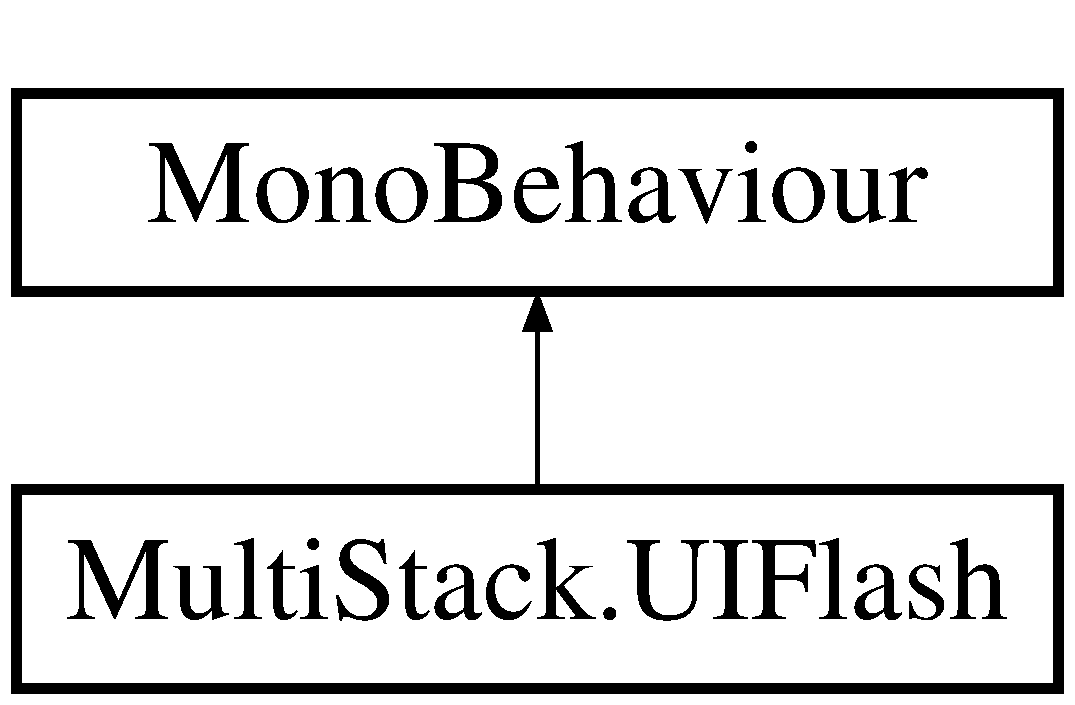
\includegraphics[height=2.000000cm]{class_multi_stack_1_1_u_i_flash}
\end{center}
\end{figure}
\subsection*{Public Member Functions}
\begin{DoxyCompactItemize}
\item 
void \hyperlink{class_multi_stack_1_1_u_i_flash_ae2b952342c47eeac57747601a724368c}{Callback\+On\+U\+I\+Flash\+Complete} (\hyperlink{namespace_multi_stack_a4bd4097b52deebcafccf5815a8495960}{Call\+Back} callback)
\begin{DoxyCompactList}\small\item\em Add a callback delegate to be invoked when the U\+I flash is complete. \end{DoxyCompactList}\item 
void \hyperlink{class_multi_stack_1_1_u_i_flash_a9c6d28d75576441b49a23682378c8411}{Game\+Over\+U\+I\+Flash\+In\+Seconds} (float seconds)
\begin{DoxyCompactList}\small\item\em Games the over user interface flash. \end{DoxyCompactList}\end{DoxyCompactItemize}
\subsection*{Public Attributes}
\begin{DoxyCompactItemize}
\item 
bool \hyperlink{class_multi_stack_1_1_u_i_flash_a520d1f1f11407f2c7feb9d790c659854}{is\+Menu}
\begin{DoxyCompactList}\small\item\em Overlay behaviour is different for menu and game scene. For menu, the overlay is less translucent. \end{DoxyCompactList}\end{DoxyCompactItemize}


\subsection{Detailed Description}
User interface flash. Acts as an overlay for the main menu and gameplay scene. 



\subsection{Member Function Documentation}
\hypertarget{class_multi_stack_1_1_u_i_flash_ae2b952342c47eeac57747601a724368c}{}\index{Multi\+Stack\+::\+U\+I\+Flash@{Multi\+Stack\+::\+U\+I\+Flash}!Callback\+On\+U\+I\+Flash\+Complete@{Callback\+On\+U\+I\+Flash\+Complete}}
\index{Callback\+On\+U\+I\+Flash\+Complete@{Callback\+On\+U\+I\+Flash\+Complete}!Multi\+Stack\+::\+U\+I\+Flash@{Multi\+Stack\+::\+U\+I\+Flash}}
\subsubsection[{Callback\+On\+U\+I\+Flash\+Complete(\+Call\+Back callback)}]{\setlength{\rightskip}{0pt plus 5cm}void Multi\+Stack.\+U\+I\+Flash.\+Callback\+On\+U\+I\+Flash\+Complete (
\begin{DoxyParamCaption}
\item[{{\bf Call\+Back}}]{callback}
\end{DoxyParamCaption}
)}\label{class_multi_stack_1_1_u_i_flash_ae2b952342c47eeac57747601a724368c}


Add a callback delegate to be invoked when the U\+I flash is complete. 


\begin{DoxyParams}{Parameters}
{\em callback} & Callback.\\
\hline
\end{DoxyParams}
\hypertarget{class_multi_stack_1_1_u_i_flash_a9c6d28d75576441b49a23682378c8411}{}\index{Multi\+Stack\+::\+U\+I\+Flash@{Multi\+Stack\+::\+U\+I\+Flash}!Game\+Over\+U\+I\+Flash\+In\+Seconds@{Game\+Over\+U\+I\+Flash\+In\+Seconds}}
\index{Game\+Over\+U\+I\+Flash\+In\+Seconds@{Game\+Over\+U\+I\+Flash\+In\+Seconds}!Multi\+Stack\+::\+U\+I\+Flash@{Multi\+Stack\+::\+U\+I\+Flash}}
\subsubsection[{Game\+Over\+U\+I\+Flash\+In\+Seconds(float seconds)}]{\setlength{\rightskip}{0pt plus 5cm}void Multi\+Stack.\+U\+I\+Flash.\+Game\+Over\+U\+I\+Flash\+In\+Seconds (
\begin{DoxyParamCaption}
\item[{float}]{seconds}
\end{DoxyParamCaption}
)}\label{class_multi_stack_1_1_u_i_flash_a9c6d28d75576441b49a23682378c8411}


Games the over user interface flash. 



\subsection{Member Data Documentation}
\hypertarget{class_multi_stack_1_1_u_i_flash_a520d1f1f11407f2c7feb9d790c659854}{}\index{Multi\+Stack\+::\+U\+I\+Flash@{Multi\+Stack\+::\+U\+I\+Flash}!is\+Menu@{is\+Menu}}
\index{is\+Menu@{is\+Menu}!Multi\+Stack\+::\+U\+I\+Flash@{Multi\+Stack\+::\+U\+I\+Flash}}
\subsubsection[{is\+Menu}]{\setlength{\rightskip}{0pt plus 5cm}bool Multi\+Stack.\+U\+I\+Flash.\+is\+Menu}\label{class_multi_stack_1_1_u_i_flash_a520d1f1f11407f2c7feb9d790c659854}


Overlay behaviour is different for menu and game scene. For menu, the overlay is less translucent. 



The documentation for this class was generated from the following file\+:\begin{DoxyCompactItemize}
\item 
Multiplayer\+Stacker/\+Scripts/\+U\+I/U\+I\+Flash.\+cs\end{DoxyCompactItemize}

\hypertarget{class_multi_stack_1_1_utilities}{}\section{Multi\+Stack.\+Utilities Class Reference}
\label{class_multi_stack_1_1_utilities}\index{Multi\+Stack.\+Utilities@{Multi\+Stack.\+Utilities}}


Useful methods used by a number of classes.  


Inheritance diagram for Multi\+Stack.\+Utilities\+:\begin{figure}[H]
\begin{center}
\leavevmode
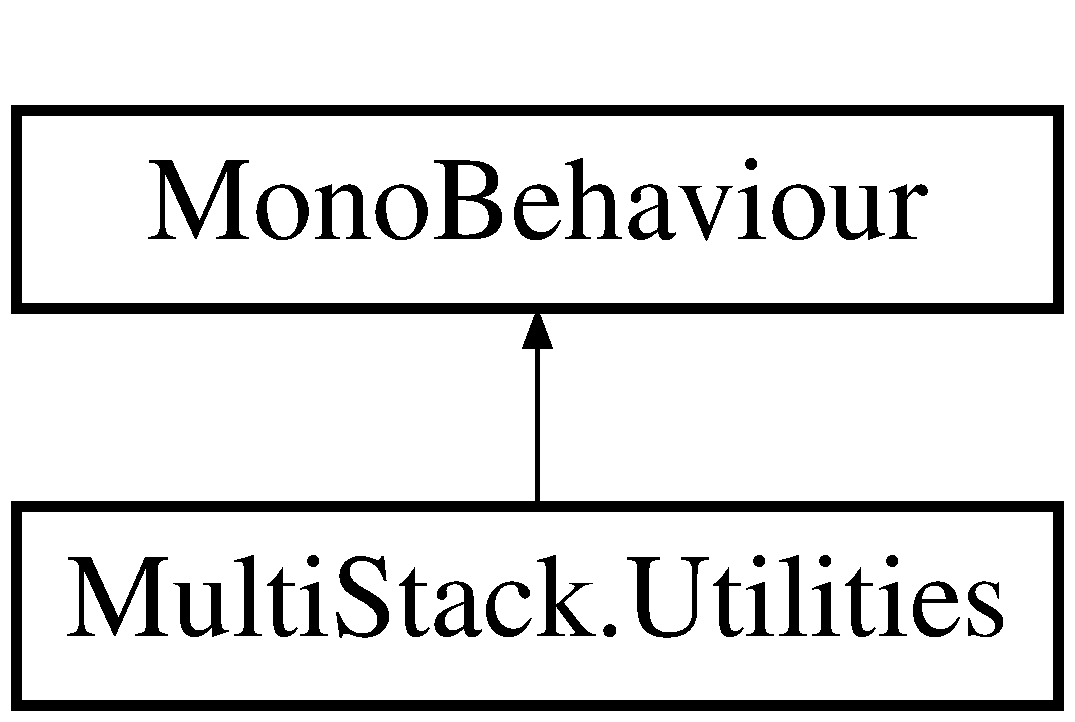
\includegraphics[height=2.000000cm]{class_multi_stack_1_1_utilities}
\end{center}
\end{figure}
\subsection*{Public Member Functions}
\begin{DoxyCompactItemize}
\item 
Quaternion \hyperlink{class_multi_stack_1_1_utilities_a68f6db0cf3e49859e5c29981d540f793}{Get\+Random\+Rotation2\+D} ()
\begin{DoxyCompactList}\small\item\em Gets a random 2d rotation (z-\/axis). \end{DoxyCompactList}\item 
void \hyperlink{class_multi_stack_1_1_utilities_aea64387ce108227f309cf3316a9a097c}{Invoke\+Method\+Every\+Seconds} (\hyperlink{namespace_multi_stack_a4bd4097b52deebcafccf5815a8495960}{Call\+Back} method, float seconds)
\begin{DoxyCompactList}\small\item\em Invokes the delegate method at a time interval specified by seconds. \end{DoxyCompactList}\end{DoxyCompactItemize}
\subsection*{Properties}
\begin{DoxyCompactItemize}
\item 
static \hyperlink{class_multi_stack_1_1_utilities}{Utilities} \hyperlink{class_multi_stack_1_1_utilities_a5565570f4adb8534d282ce1e0835f2e0}{instance}\hspace{0.3cm}{\ttfamily  \mbox{[}get\mbox{]}}
\begin{DoxyCompactList}\small\item\em Gets the instance of this class. Only one instance exists. Provides static access from any class. \end{DoxyCompactList}\end{DoxyCompactItemize}


\subsection{Detailed Description}
Useful methods used by a number of classes. 



\subsection{Member Function Documentation}
\hypertarget{class_multi_stack_1_1_utilities_a68f6db0cf3e49859e5c29981d540f793}{}\index{Multi\+Stack\+::\+Utilities@{Multi\+Stack\+::\+Utilities}!Get\+Random\+Rotation2\+D@{Get\+Random\+Rotation2\+D}}
\index{Get\+Random\+Rotation2\+D@{Get\+Random\+Rotation2\+D}!Multi\+Stack\+::\+Utilities@{Multi\+Stack\+::\+Utilities}}
\subsubsection[{Get\+Random\+Rotation2\+D()}]{\setlength{\rightskip}{0pt plus 5cm}Quaternion Multi\+Stack.\+Utilities.\+Get\+Random\+Rotation2\+D (
\begin{DoxyParamCaption}
{}
\end{DoxyParamCaption}
)}\label{class_multi_stack_1_1_utilities_a68f6db0cf3e49859e5c29981d540f793}


Gets a random 2d rotation (z-\/axis). 

\begin{DoxyReturn}{Returns}
The random rotation.
\end{DoxyReturn}
\hypertarget{class_multi_stack_1_1_utilities_aea64387ce108227f309cf3316a9a097c}{}\index{Multi\+Stack\+::\+Utilities@{Multi\+Stack\+::\+Utilities}!Invoke\+Method\+Every\+Seconds@{Invoke\+Method\+Every\+Seconds}}
\index{Invoke\+Method\+Every\+Seconds@{Invoke\+Method\+Every\+Seconds}!Multi\+Stack\+::\+Utilities@{Multi\+Stack\+::\+Utilities}}
\subsubsection[{Invoke\+Method\+Every\+Seconds(\+Call\+Back method, float seconds)}]{\setlength{\rightskip}{0pt plus 5cm}void Multi\+Stack.\+Utilities.\+Invoke\+Method\+Every\+Seconds (
\begin{DoxyParamCaption}
\item[{{\bf Call\+Back}}]{method, }
\item[{float}]{seconds}
\end{DoxyParamCaption}
)}\label{class_multi_stack_1_1_utilities_aea64387ce108227f309cf3316a9a097c}


Invokes the delegate method at a time interval specified by seconds. 


\begin{DoxyParams}{Parameters}
{\em method} & Method.\\
\hline
{\em seconds} & Time between each method call.\\
\hline
\end{DoxyParams}


\subsection{Property Documentation}
\hypertarget{class_multi_stack_1_1_utilities_a5565570f4adb8534d282ce1e0835f2e0}{}\index{Multi\+Stack\+::\+Utilities@{Multi\+Stack\+::\+Utilities}!instance@{instance}}
\index{instance@{instance}!Multi\+Stack\+::\+Utilities@{Multi\+Stack\+::\+Utilities}}
\subsubsection[{instance}]{\setlength{\rightskip}{0pt plus 5cm}{\bf Utilities} Multi\+Stack.\+Utilities.\+instance\hspace{0.3cm}{\ttfamily [static]}, {\ttfamily [get]}}\label{class_multi_stack_1_1_utilities_a5565570f4adb8534d282ce1e0835f2e0}


Gets the instance of this class. Only one instance exists. Provides static access from any class. 

The instance.

The documentation for this class was generated from the following file\+:\begin{DoxyCompactItemize}
\item 
Multiplayer\+Stacker/\+Scripts/\+Helpers/Utilities.\+cs\end{DoxyCompactItemize}

%--- End generated contents ---

% Index
\backmatter
\newpage
\phantomsection
\clearemptydoublepage
\addcontentsline{toc}{chapter}{Index}
\printindex

\end{document}
